\documentclass[12pt,a4paper]{article}
\usepackage{fontspec}
\usepackage[vietnamese]{babel}
\usepackage{geometry}
\usepackage{enumitem}
\usepackage{hyperref}
\usepackage{xcolor}
\usepackage{graphicx}
\usepackage{float}
\usepackage{tikz}
\geometry{margin=2.5cm}
\hypersetup{colorlinks=true,urlcolor=blue}
\setlist[itemize]{itemsep=3pt,topsep=4pt}
\title{Hệ thống huyệt theo kinh lạc}
\date{\today}
\begin{document}
\begin{titlepage}
\thispagestyle{empty}
\centering
\vspace*{1.2cm}
\begin{flushleft}
{\small\bfseries\color{blue!55!black} TÀI LIỆU TRA CỨU\par}
\vspace{0.25cm}
{\color{blue!55!black}\rule{\textwidth}{1.4pt}\par}
\end{flushleft}

\vspace{1.1cm}
\vspace{1.2cm}
{\Huge\bfseries\color{blue!55!black} HỆ THỐNG HUYỆT\par}
\vspace{0.2cm}
{\Huge\bfseries THEO KINH LẠC\par}
\vspace{0.65cm}
{\large\color{black!70} Các kinh chính, mạch Đốc, mạch Nhâm\\
và huyệt ngoài kinh\par}

\vfill
{\color{teal!70!black}\rule{0.28\textwidth}{1pt}\par}
\vspace{0.4cm}
{\large\bfseries\color{blue!55!black}\today\par}
\vspace*{1.2cm}
\end{titlepage}
\clearpage
\tableofcontents
\clearpage

\clearpage
\section{Kinh Thủ Dương Minh Đại Trường}
\begin{description}
  \item[Tên kinh:] Thủ Dương Minh Đại Trường (Hand Yangming, Large Intestine Channel).
  \item[Hán tự và phiên âm:] 手陽明大腸經; shǒu yáng míng dà cháng jīng.
  \item[Thời gian hoạt động:] 5--7 giờ sáng.
  \item[Ngũ hành:] Kim (Metal).
  \item[Kinh biểu lý:] Thủ Thái Âm Phế (Hand Taiyin, Lung Channel).
\end{description}

\subsection*{Đường đi}
Kinh Đại Trường khởi đầu tại Thương Dương (LI 1) và đi lên đến Kiên Ngung (LI 15). Từ đây, kinh chạy dọc bờ trước cánh tay trên, qua Bỉnh Phong (SI 12), rồi đến Đại Chùy (GV 14), vượt qua vai và tới hõm thượng đòn tại Khuyết Bồn (ST 12), sau đó chia thành hai nhánh. Nhánh thứ nhất đi vào trong cơ thể, qua tạng Phế rồi đến tạng Đại Trường. Nhánh thứ hai đi lên cổ, qua cơ ức-đòn-chũm, Thiên Đỉnh (LI 17) và Phù Đột (LI 18), qua má tại Địa Thương (ST 4), vào răng và lợi hàm dưới, vòng quanh môi trên đến Nhân Trung (GV 26), bắt chéo sang phía đối diện và tới Nghinh Hương (LI 20), nơi kinh nối với kinh Vị.

\subsection*{Chỉ định của kinh}
\begin{itemize}
  \item Tiêu chảy, lỵ.
  \item Đau răng.
  \item Đau cổ, phần trước vai và dọc bờ trước nhóm cơ duỗi của chi trên.
\end{itemize}

\subsection*{Ứng dụng của kinh}
\begin{itemize}
  \item Tiếp nhận chất thải từ Tiểu Trường.
  \item Chuyển hóa phân và tái hấp thu dịch.
\end{itemize}

\subsection*{Phương pháp cân bằng}
\begin{itemize}
  \item Hệ thống 1: Túc Dương Minh Vị (Foot Yangming, ST Channel).
  \item Hệ thống 2: Túc Quyết Âm Can (Foot Jueyin, LR Channel).
  \item Hệ thống 3: Thủ Thái Âm Phế (Hand Taiyin, LU Channel).
  \item Hệ thống 4: Túc Thiếu Âm Thận (Foot Shaoyin, KI Channel).
  \item Hệ thống 5: Túc Dương Minh Vị (Foot Yangming, ST Channel).
\end{itemize}

\subsection*{Các huyệt đặc biệt trên kinh}
\begin{description}
  \item[Ngũ du huyệt:] Tỉnh (Jing-Well) -- LI 1; Huỳnh (Ying-Spring) -- LI 2; Du (Shu-Stream) -- LI 3; Kinh (Jing-River) -- LI 5; Hợp (He-Sea) -- LI 11.
  \item[Nguyên huyệt:] LI 4.
  \item[Lạc huyệt:] LI 6.
  \item[Khích huyệt:] LI 7.
  \item[Mộ trước:] Thiên Khu (ST 25).
  \item[Du sau:] Đại Trường Du (BL 25).
  \item[Hạ hợp huyệt:] Thượng Cự Hư (ST 37).
  \item[Huyệt mẹ:] LI 11.
  \item[Huyệt con:] LI 2.
  \item[Huyệt nhập:] LI 4.
  \item[Huyệt xuất:] LI 20.
\end{description}

\subsection{LI 1 - Thương Dương (Shangyang)}
\subsection*{Thông tin cơ bản}
\begin{description}
  \item[Hán tự và phiên âm:] 商陽; shāng yáng.
  \item[Ý nghĩa tên:] Nguồn không giải thích ý nghĩa tên (The source does not explain the name).
  \item[Ngũ hành/thuộc tính:] Kim (Metal Element); Kim Dương (Metal Yang).
  \item[Phân loại:] Huyệt Tỉnh (Jing-Well), huyệt Kim của kinh Đại Trường.
\end{description}
\subsection*{Vị trí}
Ở bờ quay (radial side) ngón trỏ, cách góc móng khoảng \(0{,}1\) thốn về phía sau (posterior).
\begin{figure}[H]\centering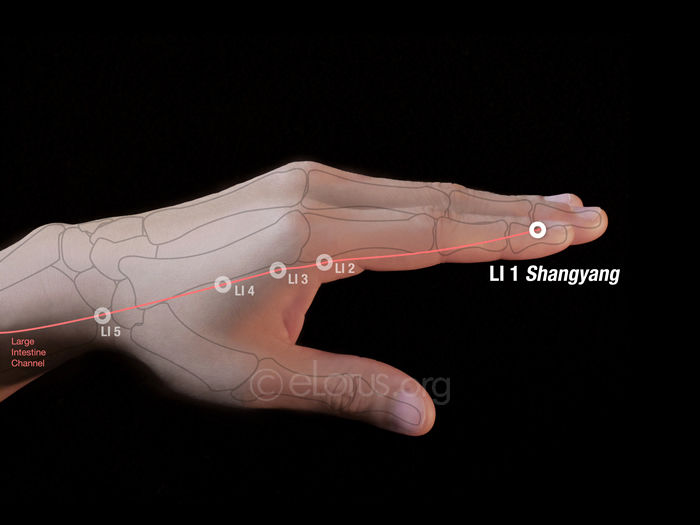
\includegraphics[width=\linewidth]{LI_1.jpg}\caption{Hình minh họa huyệt LI 1.}\end{figure}
\subsection*{Chỉ định}
Đau răng, sưng vùng dưới hàm, đau họng; tê các ngón tay; bệnh sốt kèm vô hãn (anhidrosis), mất ý thức.
\subsection*{Ứng dụng}
Thanh nhiệt, giảm sưng, giảm đau; làm tỉnh lại.
\subsection*{Thủ thuật}
Châm xiên \(0{,}1\) thốn (cun), hoặc chích lể cho chảy máu.
\subsection*{Ghi chú đặc biệt}
Huyệt Tỉnh thuộc hành Kim của kinh Đại Trường.

\subsection{LI 2 - Nhị Gian (Erjian)}
\subsection*{Thông tin cơ bản}
\begin{description}\item[Hán tự và phiên âm:] 二間; èr jiān.\item[Ngũ hành:] Thủy (Water).\item[Ý nghĩa tên:] Khoảng thứ hai (Second Space, Second Interval).\item[Phân loại:] Huyệt Huỳnh (Ying-Spring), thuộc Thủy.\end{description}
\subsection*{Vị trí}
Ở bờ quay ngón trỏ, trong chỗ lõm phía xa (distal) khớp bàn-ngón thứ hai (2nd MCP joint); định vị khi ngón tay hơi gấp.
\begin{figure}[H]\centering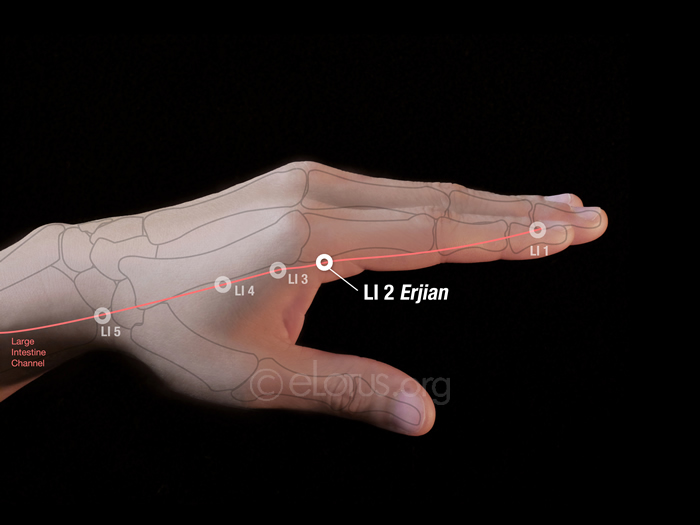
\includegraphics[width=\linewidth]{LI_2.jpg}\caption{Hình minh họa huyệt LI 2.}\end{figure}
\subsection*{Chỉ định}Nhìn mờ; chảy máu cam, đau răng, đau họng; bệnh sốt.
\subsection*{Ứng dụng}Trừ phong, thanh nhiệt; giảm sưng.
\subsection*{Thủ thuật}Châm thẳng \(0{,}2\)--\(0{,}3\) thốn.
\subsection*{Ghi chú đặc biệt}Huyệt Huỳnh thuộc Thủy của kinh Đại Trường.

\subsection{LI 3 - Tam Gian (Sanjian)}
\subsection*{Thông tin cơ bản}
\begin{description}\item[Hán tự và phiên âm:] 三間; sān jiān.\item[Ngũ hành:] Mộc (Wood).\item[Ý nghĩa tên:] Khoảng thứ ba (Third Space, Third Interval).\item[Phân loại:] Huyệt Du (Shu-Stream), thuộc Mộc.\end{description}
\subsection*{Vị trí}Khi nắm hờ bàn tay, huyệt ở bờ quay ngón trỏ, trong chỗ lõm phía gần (proximal) đầu xương bàn tay thứ hai.
\begin{figure}[H]\centering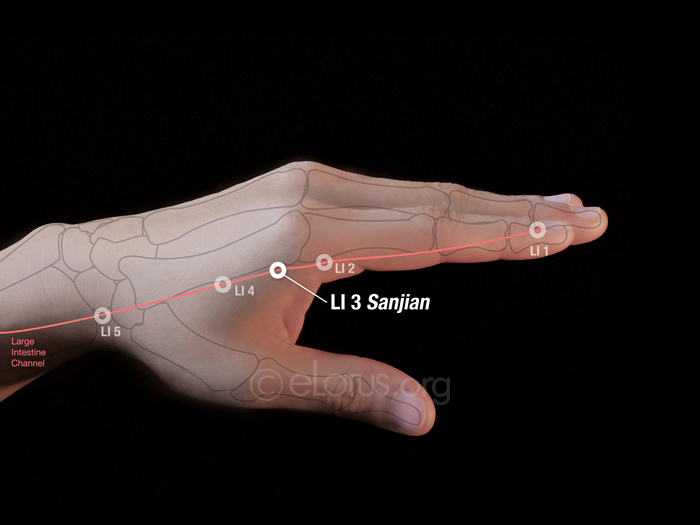
\includegraphics[width=\linewidth]{LI_3.jpg}\caption{Hình minh họa huyệt LI 3.}\end{figure}
\subsection*{Chỉ định}Đau răng, đau họng; đau mắt; các ngón tay và mu bàn tay đỏ, sưng.
\subsection*{Ứng dụng}Khu phong, thanh nhiệt ở biểu; thanh nhiệt, lợi họng và răng; làm sáng mắt.
\subsection*{Thủ thuật}Châm thẳng \(0{,}5\)--\(0{,}8\) thốn.
\subsection*{Ghi chú đặc biệt}Huyệt Du thuộc Mộc của kinh Đại Trường.

\subsection{LI 4 - Hợp Cốc (Hegu)}
\subsection*{Thông tin cơ bản}\begin{description}\item[Hán tự và phiên âm:] 合谷; hé gǔ.\item[Ý nghĩa tên:] Thung lũng hội tụ (Union Valley, Junction Valley, Joining Valley).\item[Phân loại:] Nguyên huyệt (Yuan-Source); huyệt nhập (Entry Point) của kinh Đại Trường; huyệt chủ vùng mặt và miệng (Command Point).\end{description}
\subsection*{Vị trí}Ở mu bàn tay, giữa xương bàn tay thứ nhất và thứ hai, khoảng giữa thân xương bàn tay thứ hai về phía bờ quay. Cách định vị khác: đặt nếp gấp ngang của khớp liên đốt ngón cái lên bờ kẽ giữa ngón cái và ngón trỏ của bàn tay kia; huyệt ở vị trí đầu ngón cái chạm vào.
\begin{figure}[H]\centering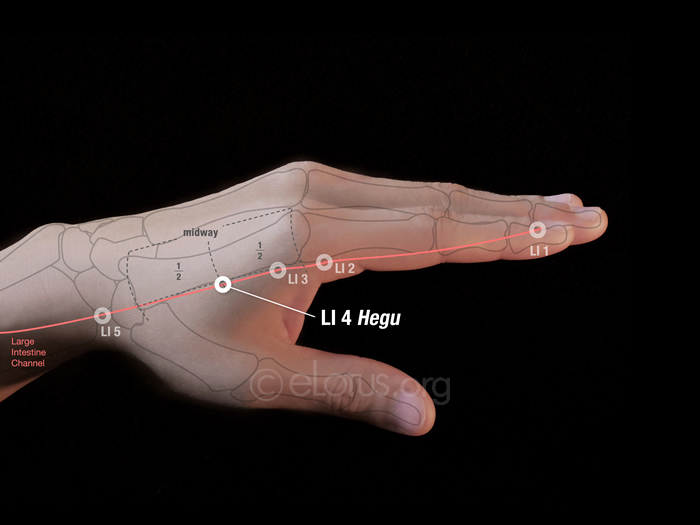
\includegraphics[width=\linewidth]{LI_4.jpg}\caption{Hình minh họa huyệt LI 4.}\end{figure}
\subsection*{Chỉ định}Đau đầu, đau cổ; mắt đỏ, sưng hoặc đau; chảy máu cam, nghẹt mũi, chảy nước mũi, đau họng, viêm tuyến mang tai, cứng khít hàm, liệt mặt, sưng mặt; bệnh sốt kèm vô hãn hoặc ra mồ hôi; đau bụng, lỵ, táo bón; vô kinh, chuyển dạ muộn, co giật ở trẻ nhỏ; đau, yếu hoặc suy giảm vận động chi trên.
\subsection*{Chống chỉ định}Chống chỉ định trong thai kỳ.
\subsection*{Ứng dụng}Điều hòa vệ khí (wei/defensive qi), kiểm soát mồ hôi, khu phong, giải biểu; điều hòa vùng mặt, mắt, mũi, miệng và tai; thông kinh, giảm đau; an thần; bổ và điều hòa khí.
\subsection*{Thủ thuật}Châm thẳng \(0{,}5\)--\(1\) thốn.
\subsection*{Ghi chú đặc biệt}Nguyên huyệt và huyệt nhập của kinh Đại Trường; huyệt chủ vùng mặt và miệng.

\subsection{LI 5 - Dương Khê (Yangxi)}
\subsection*{Thông tin cơ bản}\begin{description}\item[Hán tự và phiên âm:] 陽谿; yáng xī.\item[Ngũ hành:] Hỏa (Fire).\item[Ý nghĩa tên:] Khe suối Dương (Yang Ravine, Yang Stream).\item[Phân loại:] Huyệt Kinh (Jing-River), thuộc Hỏa.\end{description}
\subsection*{Vị trí}Ở phía quay cổ tay. Khi ngón cái duỗi/ngửa lên, huyệt nằm trong chỗ lõm giữa gân cơ duỗi dài và cơ duỗi ngắn ngón cái.
\begin{figure}[H]\centering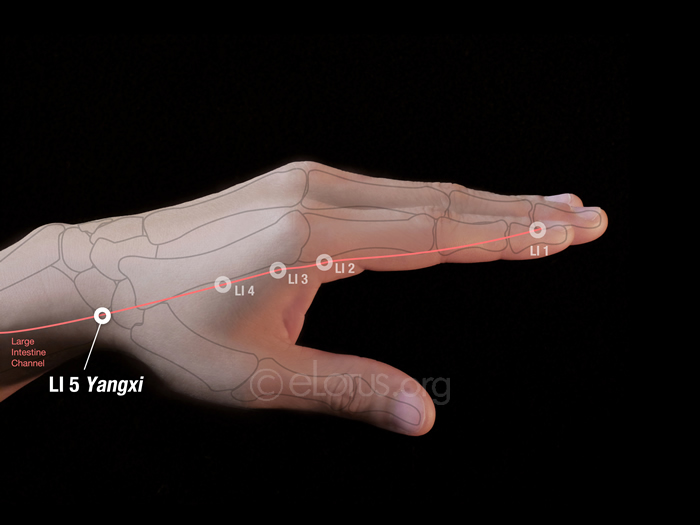
\includegraphics[width=\linewidth]{LI_5.jpg}\caption{Hình minh họa huyệt LI 5.}\end{figure}
\subsection*{Chỉ định}Đau đầu; mắt đỏ, đau và sưng; đau răng, đau họng; đau cổ tay.
\subsection*{Ứng dụng}Khu phong, tán nhiệt, giảm đau, thanh hỏa Dương Minh; lợi khớp cổ tay.
\subsection*{Thủ thuật}Châm thẳng \(0{,}3\)--\(0{,}5\) thốn.
\subsection*{Ghi chú đặc biệt}Huyệt Kinh thuộc Hỏa của kinh Đại Trường.

\subsection{LI 6 - Thiên Lịch (Pianli)}
\subsection*{Thông tin cơ bản}\begin{description}\item[Hán tự và phiên âm:] 偏歴; piān lì.\item[Ý nghĩa tên:] Đường đi lệch (Veering Passageway, Slanting Passage).\item[Phân loại:] Lạc huyệt (Luo-Connecting) của kinh Đại Trường.\end{description}
\subsection*{Vị trí}Gấp khuỷu tay, để mặt quay của cẳng tay hướng lên; huyệt nằm trên đường nối Dương Khê (LI 5) với Khúc Trì (LI 11), cách Dương Khê 3 thốn về phía gần (proximal).
\begin{figure}[H]\centering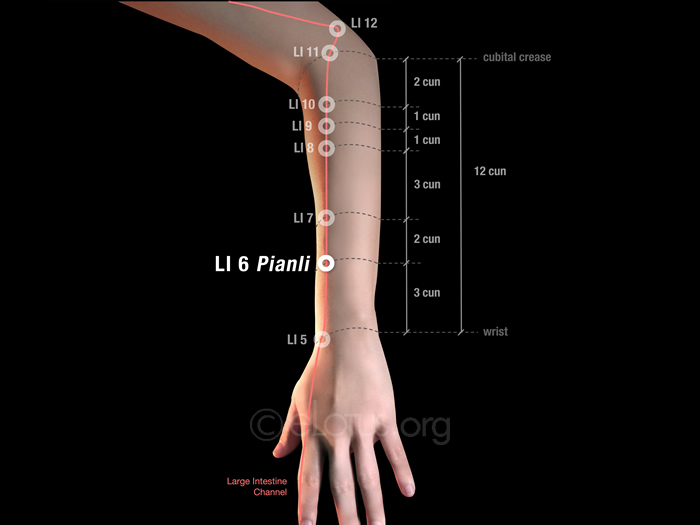
\includegraphics[width=\linewidth]{LI_6.jpg}\caption{Hình minh họa huyệt LI 6.}\end{figure}
\subsection*{Chỉ định}Phù; mắt đỏ, ù tai, điếc, chảy máu cam, đau họng; đau nhức bàn tay và cánh tay.
\subsection*{Ứng dụng}Khai thông và điều hòa thủy đạo; khu phong, thanh nhiệt.
\subsection*{Thủ thuật}Châm thẳng hoặc xiên \(0{,}5\)--\(1\) thốn.
\subsection*{Ghi chú đặc biệt}Lạc huyệt của kinh Đại Trường.

\subsection{LI 7 - Ôn Lưu (Wenliu)}
\subsection*{Thông tin cơ bản}\begin{description}\item[Hán tự và phiên âm:] 溫溜; wēn liū.\item[Ý nghĩa tên:] Dòng chảy ấm (Warm Dwelling, Warm Flow).\item[Phân loại:] Khích huyệt (Xi-Cleft) của kinh Đại Trường.\end{description}
\subsection*{Vị trí}Gấp khuỷu tay, để mặt quay của cẳng tay hướng lên; huyệt nằm trên đường nối Dương Khê (LI 5) với Khúc Trì (LI 11), cách Dương Khê 5 thốn về phía gần (proximal).
\begin{figure}[H]\centering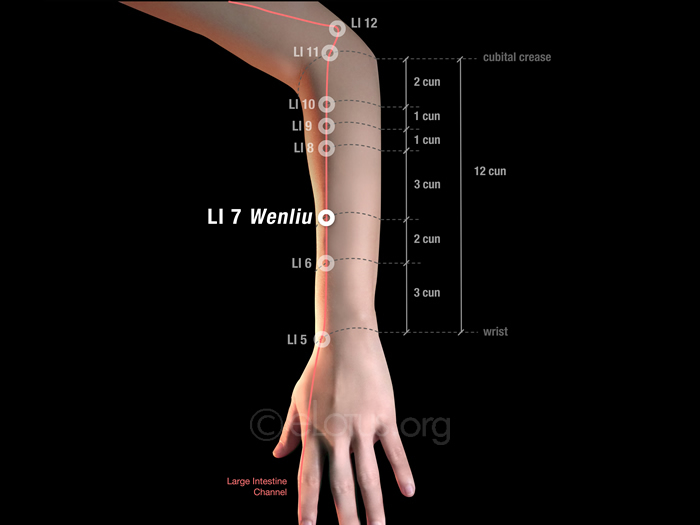
\includegraphics[width=\linewidth]{LI_7.jpg}\caption{Hình minh họa huyệt LI 7.}\end{figure}
\subsection*{Chỉ định}Đau và viêm miệng, lưỡi, răng; đau đầu, sưng mặt, đau họng; tiếng sôi bụng, đau bụng; đau vai và cánh tay.
\subsection*{Ứng dụng}Thanh nhiệt; giảm đau, khu phong, lợi họng; điều hòa ruột và dạ dày.
\subsection*{Thủ thuật}Châm thẳng \(0{,}5\)--\(1\) thốn.
\subsection*{Ghi chú đặc biệt}Khích huyệt của kinh Đại Trường.

\subsection{LI 8 - Hạ Liêm (Xialian)}
\subsection*{Thông tin cơ bản}\begin{description}\item[Hán tự và phiên âm:] 下廉; xià lián.\item[Ý nghĩa tên:] Bờ/góc dưới (Lower Ridge, Lower Corner, Lower Integrity, Lower Angle).\end{description}
\subsection*{Vị trí}Gấp khuỷu tay, để mặt quay cẳng tay hướng lên; huyệt nằm trên đường nối Dương Khê (LI 5) với Khúc Trì (LI 11), cách Khúc Trì 4 thốn về phía xa (distal).
\begin{figure}[H]\centering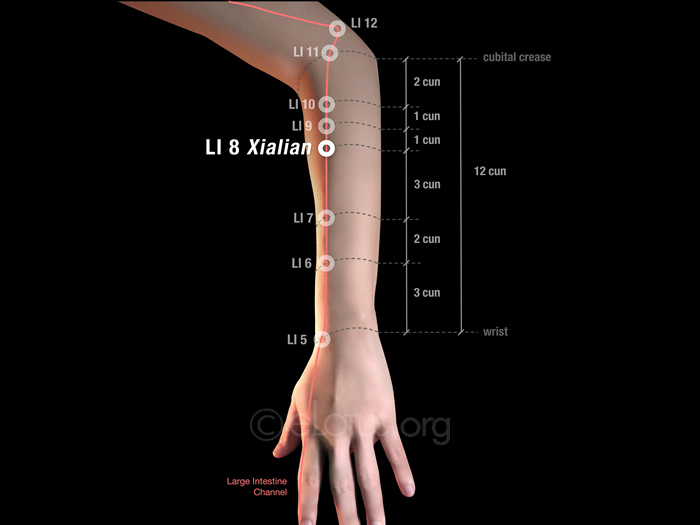
\includegraphics[width=\linewidth]{LI_8.jpg}\caption{Hình minh họa huyệt LI 8.}\end{figure}
\subsection*{Chỉ định}Đau bụng, tiếng sôi bụng; đau khuỷu tay và cánh tay, suy giảm vận động chi trên.
\subsection*{Ứng dụng}Điều hòa Tiểu Trường; khu phong, thanh nhiệt.
\subsection*{Thủ thuật}Châm thẳng \(0{,}5\)--\(1\) thốn.

\subsection{LI 9 - Thượng Liêm (Shanglian)}
\subsection*{Thông tin cơ bản}\begin{description}\item[Hán tự và phiên âm:] 上廉; shàng lián.\item[Ý nghĩa tên:] Bờ/góc trên (Upper Ridge, Upper Corner, Upper Angle, Upper Integrity).\end{description}
\subsection*{Vị trí}Gấp khuỷu tay, để mặt quay cẳng tay hướng lên; huyệt nằm trên đường nối Dương Khê (LI 5) với Khúc Trì (LI 11), cách Khúc Trì 3 thốn về phía xa (distal).
\begin{figure}[H]\centering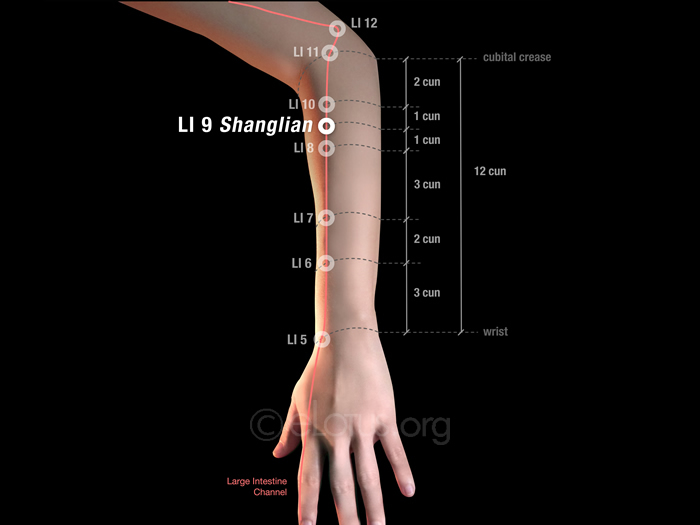
\includegraphics[width=\linewidth]{LI_9.jpg}\caption{Hình minh họa huyệt LI 9.}\end{figure}
\subsection*{Chỉ định}Tiếng sôi bụng, đau bụng; đau nhức vai và cánh tay, suy giảm vận động chi trên, tê bàn tay và cánh tay.
\subsection*{Ứng dụng}Điều hòa Đại Trường; thông kinh và giảm đau.
\subsection*{Thủ thuật}Châm thẳng \(0{,}5\)--\(1\) thốn.

\subsection{LI 10 - Thủ Tam Lý (Shousanli)}
\subsection*{Thông tin cơ bản}\begin{description}\item[Hán tự và phiên âm:] 手三里; shǒu sān lǐ.\item[Ý nghĩa tên:] Tam Lý ở cánh tay (Arm Three Li, Arm Three Miles).\end{description}
\subsection*{Vị trí}Gấp khuỷu tay, để mặt quay cẳng tay hướng lên; huyệt nằm trên đường nối Dương Khê (LI 5) với Khúc Trì (LI 11), cách Khúc Trì 2 thốn về phía xa (distal).
\begin{figure}[H]\centering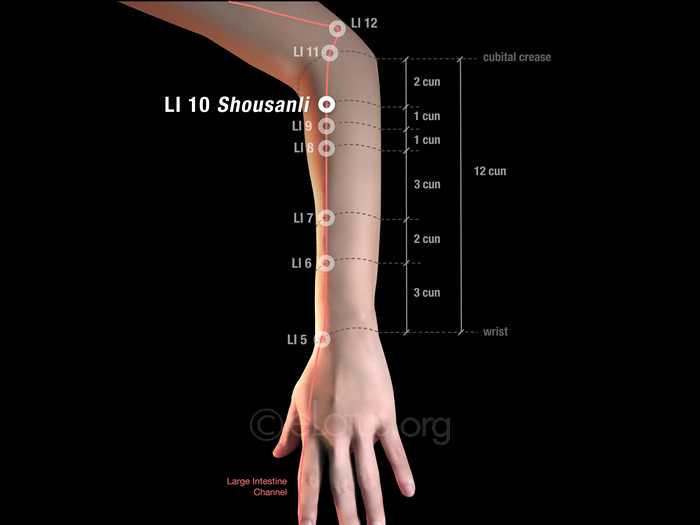
\includegraphics[width=\linewidth]{LI_10.jpg}\caption{Hình minh họa huyệt LI 10.}\end{figure}
\subsection*{Chỉ định}Suy giảm vận động chi trên, đau vai và lưng; đau bụng, nôn, tiêu chảy; đau răng, sưng má.
\subsection*{Ứng dụng}Điều hòa khí huyết; thông kinh, giảm đau; điều hòa ruột và dạ dày.
\subsection*{Thủ thuật}Châm thẳng \(0{,}8\)--\(1{,}2\) thốn.

\subsection{LI 11 - Khúc Trì (Quchi)}
\subsection*{Thông tin cơ bản}\begin{description}\item[Hán tự và phiên âm:] 曲池; qū chí.\item[Ngũ hành:] Thổ (Earth).\item[Ý nghĩa tên:] Ao ở chỗ gấp (Pool at the Bend, Pool at the Crook, Crooked Pond).\item[Phân loại:] Huyệt Hợp (He-Sea), thuộc Thổ; huyệt mẹ của kinh Đại Trường.\end{description}
\subsection*{Vị trí}Khi gấp khuỷu tay, huyệt nằm trong chỗ lõm ở đầu ngoài nếp gấp ngang khuỷu, giữa huyệt Xích Trạch (LU 5) và mỏm trên lồi cầu ngoài xương cánh tay.
\begin{figure}[H]\centering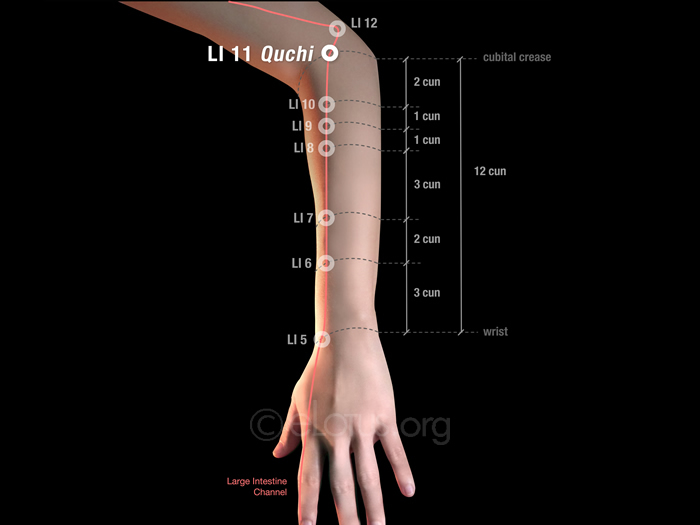
\includegraphics[width=\linewidth]{LI_11.jpg}\caption{Hình minh họa huyệt LI 11.}\end{figure}
\subsection*{Chỉ định}Đau họng, đau răng, bệnh sốt; mắt đỏ và đau; loa lịch, mề đay, ngứa da; suy giảm vận động chi trên; đau bụng, nôn, tiêu chảy.
\subsection*{Ứng dụng}Thanh nhiệt, lương huyết, khu phong, trừ thấp, giảm ngứa; điều hòa khí huyết, hoạt lạc, giảm đau.
\subsection*{Thủ thuật}Châm thẳng \(1\)--\(1{,}5\) thốn.
\subsection*{Ghi chú đặc biệt}Huyệt Hợp thuộc Thổ của kinh Đại Trường; Quỷ huyệt thứ 13 (13 Ghost Point -- Leg).

\subsection{LI 12 - Trửu Liêu (Zhouliao)}
\subsection*{Thông tin cơ bản}\begin{description}\item[Hán tự và phiên âm:] 肘髎; zhǒu liáo.\item[Ý nghĩa tên:] Hốc/khe khuỷu tay (Elbow Bone Hole, Elbow Crevice, Elbow Seam).\end{description}
\subsection*{Vị trí}Gấp khuỷu tay; huyệt nằm trong chỗ lõm cách Khúc Trì (LI 11) 1 thốn về phía gần và phía ngoài, trên bờ trong xương cánh tay (phía trên mỏm trên lồi cầu ngoài).
\begin{figure}[H]\centering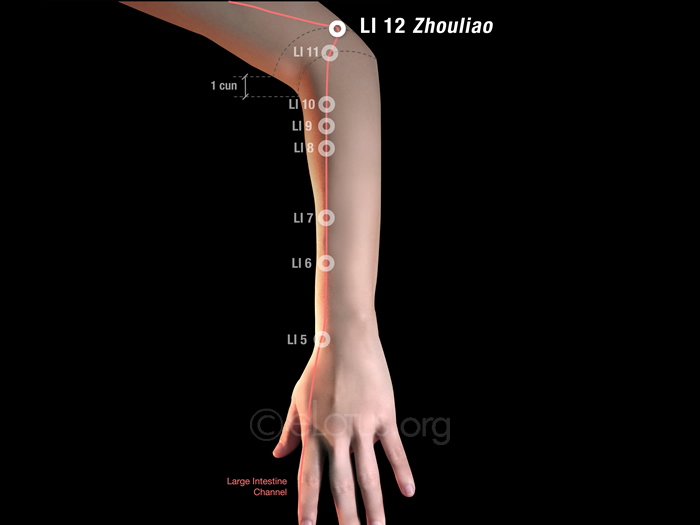
\includegraphics[width=\linewidth]{LI_12.jpg}\caption{Hình minh họa huyệt LI 12.}\end{figure}
\subsection*{Chỉ định}Đau, tê, co rút khuỷu tay và cánh tay.
\subsection*{Ứng dụng}Hoạt lạc, giảm đau; lợi khớp khuỷu.
\subsection*{Thủ thuật}Châm thẳng \(0{,}5\)--\(1\) thốn.

\subsection{LI 13 - Thủ Ngũ Lý (Shouwuli)}
\subsection*{Thông tin cơ bản}\begin{description}\item[Hán tự và phiên âm:] 手五里; shǒu wǔ lǐ.\item[Ý nghĩa tên:] Ngũ Lý ở cánh tay (Arm Five Li, Arm Five Miles, Five Measures on the Arm).\end{description}
\subsection*{Vị trí}Ở mặt ngoài cánh tay trên, trên đường nối Khúc Trì (LI 11) với Kiên Ngung (LI 15), cách Khúc Trì 3 thốn về phía gần.
\begin{figure}[H]\centering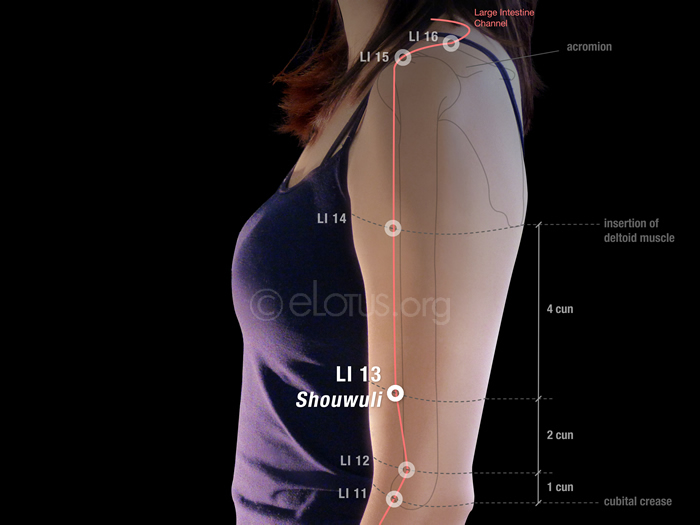
\includegraphics[width=\linewidth]{LI_13.jpg}\caption{Hình minh họa huyệt LI 13.}\end{figure}
\subsection*{Chỉ định}Co rút và đau khuỷu tay, cánh tay; loa lịch; ho.
\subsection*{Chống chỉ định/thận trọng}Tránh động mạch hoặc cơ quan (``Avoid artery or organ'').
\subsection*{Ứng dụng}Hoạt lạc, giảm đau; trừ thấp, hóa đàm; điều khí.
\subsection*{Thủ thuật}Châm thẳng \(0{,}5\)--\(1{,}5\) thốn.

\subsection{LI 14 - Tý Nhu (Binao)}
\subsection*{Thông tin cơ bản}\begin{description}\item[Hán tự và phiên âm:] 臂臑; bì nào.\item[Ý nghĩa tên:] Cánh tay trên (Upper Arm).\end{description}
\subsection*{Vị trí}Ở mặt ngoài cánh tay trên, trên đường nối Khúc Trì (LI 11) với Kiên Ngung (LI 15), cách Khúc Trì 7 thốn về phía gần, tại chỗ bám cơ delta.
\begin{figure}[H]\centering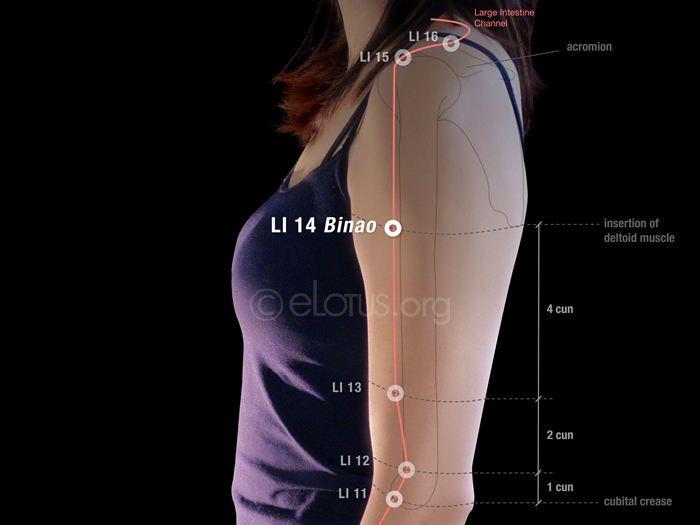
\includegraphics[width=\linewidth]{LI_14.jpg}\caption{Hình minh họa huyệt LI 14.}\end{figure}
\subsection*{Chỉ định}Đau vai và cánh tay; cứng cổ; loa lịch.
\subsection*{Ứng dụng}Thông kinh, giảm đau; hóa đàm, tiêu tích tụ.
\subsection*{Thủ thuật}Châm thẳng hoặc xiên hướng lên \(0{,}8\)--\(1{,}5\) thốn.

\subsection{LI 15 - Kiên Ngung (Jianyu)}
\subsection*{Thông tin cơ bản}\begin{description}\item[Hán tự và phiên âm:] 肩髃; jiān yú.\item[Ý nghĩa tên:] Xương vai (Shoulder Bone).\end{description}
\subsection*{Vị trí}Ở phía trước và phía dưới mỏm cùng vai, trên phần trên cơ delta. Khi dạng cánh tay hết mức, huyệt nằm trong chỗ lõm xuất hiện ở bờ trước khớp cùng-đòn.
\begin{figure}[H]\centering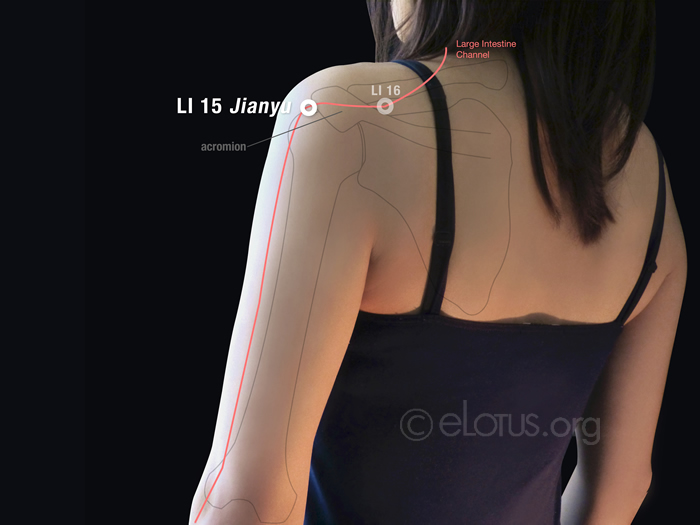
\includegraphics[width=\linewidth]{LI_15.jpg}\caption{Hình minh họa huyệt LI 15.}\end{figure}
\subsection*{Chỉ định}Đau vai và cánh tay, suy giảm vận động chi trên; rubella; loa lịch.
\subsection*{Ứng dụng}Trừ phong thấp, giảm đau, lợi khớp vai; khu phong, điều hòa khí huyết; tiêu các nốt đàm.
\subsection*{Thủ thuật}Châm thẳng hoặc xiên \(0{,}8\)--\(1{,}5\) thốn.

\subsection{LI 16 - Cự Cốt (Jugu)}
\subsection*{Thông tin cơ bản}\begin{description}\item[Hán tự và phiên âm:] 巨骨; jù gǔ.\item[Ý nghĩa tên:] Xương lớn (Great Bone).\end{description}
\subsection*{Vị trí}Ở mặt trên vai, trong chỗ lõm giữa đầu cùng vai của xương đòn và gai xương bả vai.
\begin{figure}[H]\centering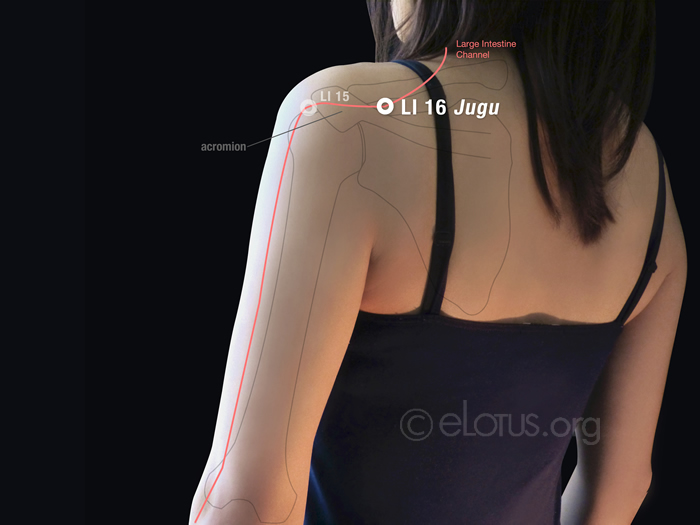
\includegraphics[width=\linewidth]{LI_16.jpg}\caption{Hình minh họa huyệt LI 16.}\end{figure}
\subsection*{Chỉ định}Đau chi trên, vai, lưng; suy giảm vận động chi trên.
\subsection*{Ứng dụng}Hoạt lạc, giảm đau, lợi khớp vai; điều hòa khí huyết; tiêu các nốt đàm.
\subsection*{Thủ thuật}Châm thẳng \(0{,}5\)--\(0{,}7\) thốn.

\subsection{LI 17 - Thiên Đỉnh (Tianding)}
\subsection*{Thông tin cơ bản}\begin{description}\item[Hán tự và phiên âm:] 天鼎; tiān dǐng.\item[Ý nghĩa tên:] Đỉnh trời (Celestial Tripod, Heaven's Tripod, Heaven's Vessel).\end{description}
\subsection*{Vị trí}Ở mặt bên cổ, tại bờ sau cơ ức-đòn-chũm, cách Phù Đột (LI 18) 1 thốn về phía dưới.
\begin{figure}[H]\centering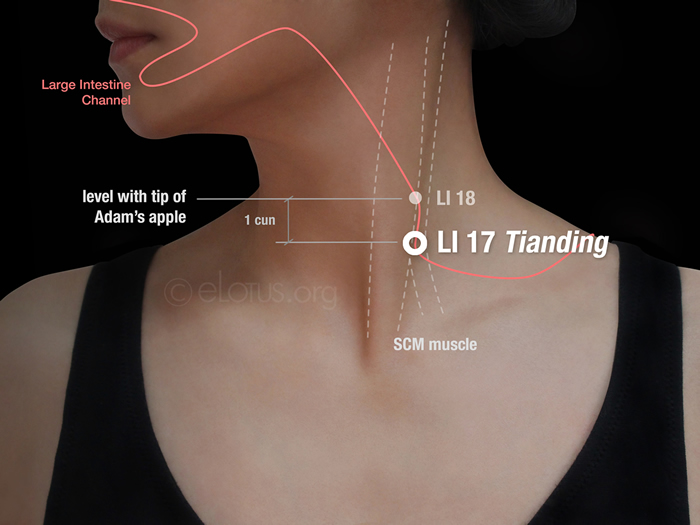
\includegraphics[width=\linewidth]{LI_17.jpg}\caption{Hình minh họa huyệt LI 17.}\end{figure}
\subsection*{Chỉ định}Đột ngột mất tiếng, đau họng; loa lịch, bướu cổ.
\subsection*{Ứng dụng}Lợi họng và tiếng nói.
\subsection*{Thủ thuật}Châm thẳng \(0{,}3\)--\(0{,}5\) thốn.

\subsection{LI 18 - Phù Đột (Futu)}
\subsection*{Thông tin cơ bản}\begin{description}\item[Hán tự và phiên âm:] 扶突; fú tū.\item[Ý nghĩa tên:] Chỗ nhô được nâng đỡ (Protuberance Assistant, Support the Prominence).\item[Phân loại:] Huyệt Thiên Song (Window of the Sky).\end{description}
\subsection*{Vị trí}Ở mặt bên cổ, ngang đầu mút sụn giáp (Adam's apple), giữa đầu ức và đầu đòn của cơ ức-đòn-chũm.
\begin{figure}[H]\centering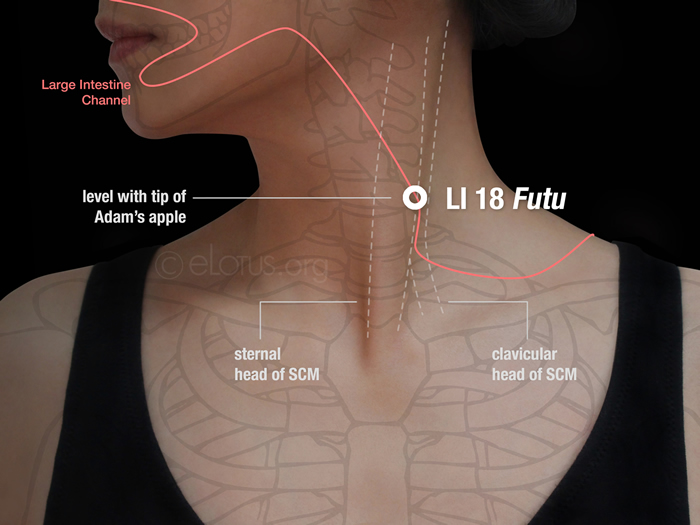
\includegraphics[width=\linewidth]{LI_18.jpg}\caption{Hình minh họa huyệt LI 18.}\end{figure}
\subsection*{Chỉ định}Ho, hen, đau họng, sưng họng, đột ngột mất tiếng; loa lịch, bướu cổ.
\subsection*{Ứng dụng}Lợi họng và tiếng nói.
\subsection*{Thủ thuật}Châm thẳng \(0{,}3\)--\(0{,}5\) thốn.

\subsection{LI 19 - Hòa Liêu (Kouheliao)}
\subsection*{Thông tin cơ bản}\begin{description}\item[Hán tự và phiên âm:] 口禾髎; kǒu hé liáo.\item[Ý nghĩa tên:] Hốc cạnh mũi-miệng (Grain Bone Hole, Mouth Grain Crevice).\end{description}
\subsection*{Vị trí}Ngay dưới bờ ngoài cánh mũi, cách Nhân Trung (GV 26) 0{,}5 thốn về phía ngoài.
\begin{figure}[H]\centering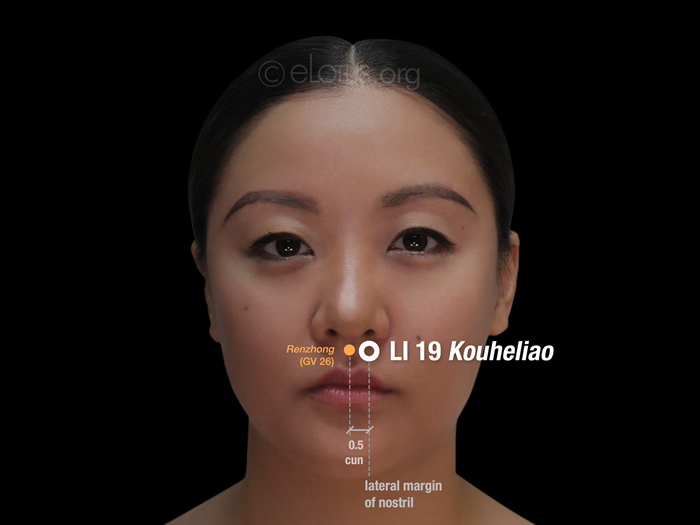
\includegraphics[width=\linewidth]{LI_19.jpg}\caption{Hình minh họa huyệt Hòa Liêu (LI 19).}\end{figure}
\subsection*{Chỉ định}Nghẹt mũi, chảy máu cam; méo miệng.
\subsection*{Chống chỉ định}Không cứu (moxibustion).
\subsection*{Ứng dụng}Khu phong, thông mũi.
\subsection*{Thủ thuật}Châm xiên \(0{,}2\)--\(0{,}5\) thốn.

\subsection{LI 20 - Nghinh Hương (Yingxiang)}
\subsection*{Thông tin cơ bản}\begin{description}\item[Hán tự và phiên âm:] 迎香; yíng xiāng.\item[Ý nghĩa tên:] Đón hương (Welcome Fragrance).\item[Phân loại:] Huyệt xuất (Exit Point) của kinh Đại Trường.\end{description}
\subsection*{Vị trí}Ở rãnh mũi-má (nasolabial groove), ngang điểm giữa bờ ngoài cánh mũi.
\begin{figure}[H]\centering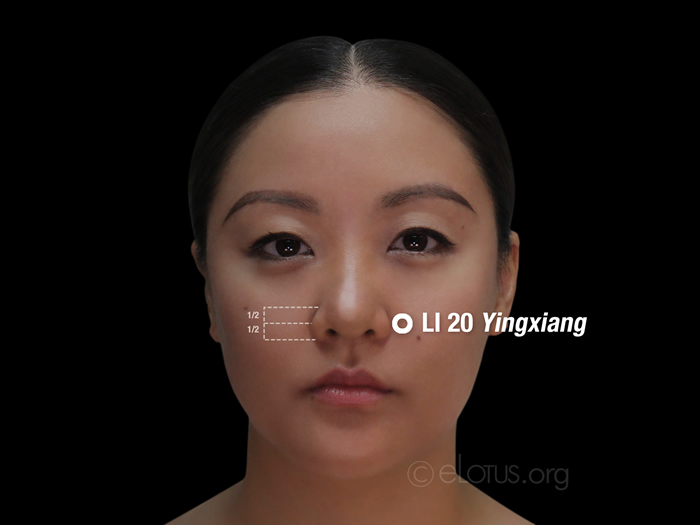
\includegraphics[width=\linewidth]{LI_20.jpg}\caption{Hình minh họa huyệt Nghinh Hương (LI 20).}\end{figure}
\subsection*{Chỉ định}Nghẹt mũi, giảm khứu giác, chảy máu cam, chảy nước mũi; méo miệng; ngứa và sưng mặt.
\subsection*{Chống chỉ định}Không cứu (moxibustion).
\subsection*{Ứng dụng}Thông mũi; khu phong ở biểu, thanh nhiệt.
\subsection*{Thủ thuật}Châm xiên hoặc dưới da \(0{,}3\)--\(0{,}5\) thốn.

\clearpage
\section{Kinh Thủ Thái Âm Phế}
\begin{description}
  \item[Tên kinh:] Thủ Thái Âm Phế (Hand Taiyin, Lung Channel).
  \item[Hán tự và phiên âm:] 手太陰肺經; shǒu tài yīn fèi jīng.
  \item[Thời gian hoạt động:] 3--5 giờ sáng.
  \item[Ngũ hành:] Kim (Metal).
  \item[Kinh biểu lý:] Thủ Dương Minh Đại Trường (Hand Yangming, Large Intestine Channel).
\end{description}

\subsection*{Đường đi}
Kinh khởi nguồn ở Trung Tiêu, đi xuống để liên hệ với Đại Trường, sau đó đi ngược lên qua Vị, xuyên cơ hoành đến Phế. Kinh tiếp tục lên họng, xuất hiện ở Trung Phủ (LU 1) và kết thúc tại Thiếu Thương (LU 11). Một nhánh tách ở Liệt Khuyết (LU 7), đi đến Hợp Cốc (LI 4) và kết thúc ở Thương Dương (LI 1), nơi nối với kinh Đại Trường.

\subsection*{Chỉ định của kinh}
\begin{itemize}
  \item Ho, hen, nghẹt mũi, khó thở và cảm mạo.
  \item Đau hoặc rối loạn dọc đường đi của kinh.
  \item Bệnh lý da, đặc biệt liên quan đến nhiệt hoặc khô.
  \item Đau hõm thượng đòn, lưng và bờ trước mặt trong cánh tay.
\end{itemize}

\subsection*{Ứng dụng của kinh}
\begin{itemize}
  \item Chủ khí và hô hấp; điều khiển kinh mạch và mạch máu.
  \item Kiểm soát chức năng tuyên phát và túc giáng của khí, dịch cơ thể; điều hòa thủy đạo.
  \item Chủ bì, phần giữa da và cơ, cùng lông trên cơ thể; khai khiếu ra mũi; tàng Phách (Corporeal Soul).
\end{itemize}

\subsection*{Phương pháp cân bằng}
\begin{enumerate}
  \item Túc Thái Âm Tỳ (Foot Taiyin, Spleen).
  \item Túc Thái Dương Bàng Quang (Foot Taiyang, Bladder).
  \item Thủ Dương Minh Đại Trường (Hand Yangming, Large Intestine).
  \item Túc Thái Dương Bàng Quang (Foot Taiyang, Bladder).
  \item Túc Quyết Âm Can (Foot Jueyin, Liver).
\end{enumerate}

\subsection*{Phân loại huyệt đặc biệt trên kinh}
\begin{itemize}
  \item Ngũ Du: Tỉnh (Jing-Well) LU 11; Huỳnh (Ying-Spring) LU 10; Du (Shu-Stream) LU 9; Kinh (Jing-River) LU 8; Hợp (He-Sea) LU 5.
  \item Nguyên huyệt (Yuan-Source): LU 9; Lạc huyệt (Luo-Connecting): LU 7; Khích huyệt (Xi-Cleft): LU 6.
  \item Mộ huyệt trước (Front-Mu): LU 1; Du huyệt sau (Back-Shu): Phế Du (BL 13).
  \item Huyệt Mẹ (Mother): LU 9; huyệt Con (Child): LU 5; huyệt Nhập (Entry): LU 1; huyệt Xuất (Exit): LU 7.
\end{itemize}

\subsection{LU 1 - Trung Phủ (Zhongfu)}
\subsection*{Thông tin cơ bản}\begin{description}\item[Hán tự và phiên âm:] 中府; zhōng fǔ.\item[Ý nghĩa tên:] Kho trung tâm (Central Treasury, Central Residence).\item[Phân loại:] Mộ huyệt trước của Phế; huyệt Nhập của kinh Phế.\end{description}
\subsection*{Vị trí}Ở khoang liên sườn thứ nhất, cách đường giữa trước 6 thốn về phía ngoài và thấp hơn Vân Môn (LU 2) 1 thốn.
\begin{figure}[H]\centering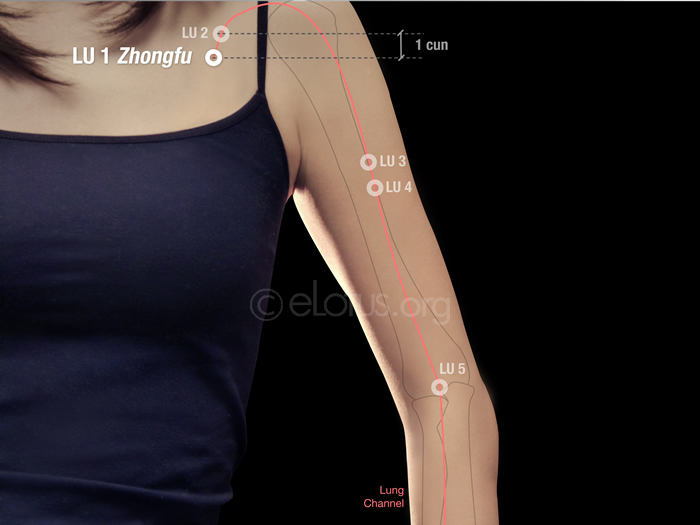
\includegraphics[width=\linewidth]{LU_1.jpg}\caption{Hình minh họa huyệt LU 1.}\end{figure}
\subsection*{Chỉ định}Ho, hen, khò khè; đau hoặc đầy tức ngực; đau vai, đau lưng.
\subsection*{Ứng dụng}Tuyên phát và túc giáng khí Phế; hóa đàm, thanh nhiệt, điều hòa thủy đạo.
\subsection*{Thủ thuật}Châm xiên 0{,}5--0{,}8 thốn hướng về phía ngoài lồng ngực. Để tránh tổn thương phổi, không châm sâu hướng vào phía trong.

\subsection{LU 2 - Vân Môn (Yunmen)}
\subsection*{Thông tin cơ bản}\begin{description}\item[Hán tự và phiên âm:] 雲門; yún mén.\item[Ý nghĩa tên:] Cửa mây (Cloud Gate, Cloud Door).\end{description}
\subsection*{Vị trí}Trong chỗ lõm dưới đầu ngoài xương đòn, cách đường giữa trước 6 thốn về phía ngoài, giữa cơ ngực lớn và cơ delta.
\begin{figure}[H]\centering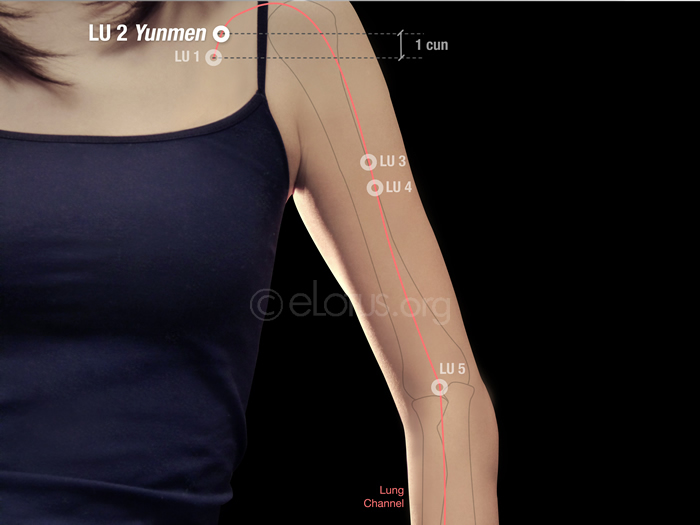
\includegraphics[width=\linewidth]{LU_2.jpg}\caption{Hình minh họa huyệt LU 2.}\end{figure}
\subsection*{Chỉ định}Ho, hen, khò khè, khó thở; đầy tức hoặc đau ngực, cảm giác nóng ở ngực; đau hoặc viêm đau vai và cánh tay.
\subsection*{Ứng dụng}Thanh nhiệt Phế, tuyên phát và túc giáng khí Phế; thanh nhiệt ở chi, thông khớp.
\subsection*{Thủ thuật}Châm xiên 0{,}5--0{,}8 thốn hướng ra ngoài lồng ngực; tránh châm sâu vào trong để phòng tổn thương phổi.

\subsection{LU 3 - Thiên Phủ (Tianfu)}
\subsection*{Thông tin cơ bản}\begin{description}\item[Hán tự và phiên âm:] 天府; tiān fǔ.\item[Ý nghĩa tên:] Kho trời (Celestial Storehouse, Heavenly Residence).\item[Phân loại:] Huyệt Thiên Song (Window of the Sky).\end{description}
\subsection*{Vị trí}Ở mặt trước-bên cánh tay trên, phía quay của cơ nhị đầu cánh tay, cách đầu trước nếp nách 3 thốn về phía dưới.
\begin{figure}[H]\centering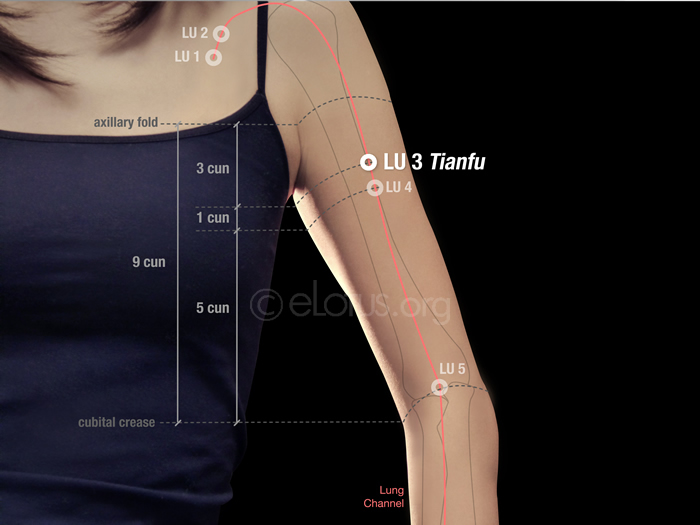
\includegraphics[width=\linewidth]{LU_3.jpg}\caption{Hình minh họa huyệt LU 3.}\end{figure}
\subsection*{Chỉ định}Hen, khò khè, ho; ho ra máu, chảy máu cam; đau mặt trong cánh tay trên.
\subsection*{Ứng dụng}Thanh nhiệt Phế, giáng khí Phế; lương huyết, chỉ huyết; an Phách (Corporeal Soul).
\subsection*{Thủ thuật}Châm thẳng 0{,}5--1 thốn.

\subsection{LU 4 - Hiệp Bạch (Xiabai)}
\subsection*{Thông tin cơ bản}\begin{description}\item[Hán tự và phiên âm:] 俠白; xiá bái.\item[Ý nghĩa tên:] Bảo vệ màu trắng (Guarding White).\end{description}
\subsection*{Vị trí}Ở mặt trước-bên cánh tay trên, phía quay cơ nhị đầu cánh tay; cách đầu trước nếp nách 4 thốn về phía dưới, hoặc cách Xích Trạch (LU 5) 5 thốn về phía trên.
\begin{figure}[H]\centering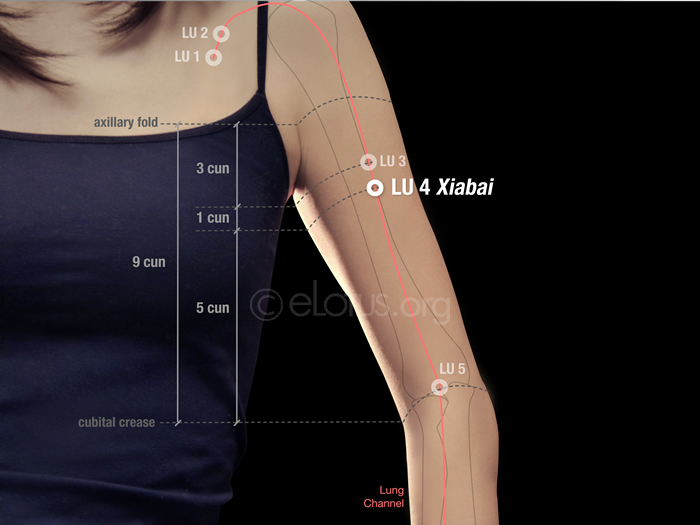
\includegraphics[width=\linewidth]{LU_4.jpg}\caption{Hình minh họa huyệt LU 4.}\end{figure}
\subsection*{Chỉ định}Ho, đầy tức ngực; đau mặt trong cánh tay trên.
\subsection*{Ứng dụng}Giáng khí Phế; điều hòa khí huyết ở ngực.
\subsection*{Thủ thuật}Châm thẳng 0{,}5--1 thốn.

\subsection{LU 5 - Xích Trạch (Chize)}
\subsection*{Thông tin cơ bản}\begin{description}\item[Hán tự và phiên âm:] 尺澤; chǐ zé.\item[Ý nghĩa tên:] Đầm ở thốn xích (Cubit Marsh).\item[Phân loại:] Ngũ hành thuộc Thủy; huyệt Hợp (He-Sea) thuộc Thủy.\end{description}
\subsection*{Vị trí}Khi khuỷu tay hơi gấp, tại nếp gấp khuỷu, trong chỗ lõm ở phía quay gân cơ nhị đầu cánh tay.
\begin{figure}[H]\centering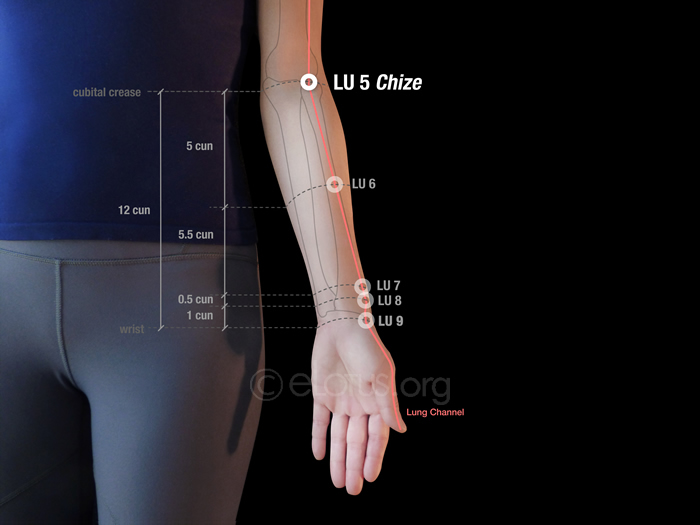
\includegraphics[width=\linewidth]{LU_5.jpg}\caption{Hình minh họa huyệt LU 5.}\end{figure}
\subsection*{Chỉ định}Ho, ho ra máu, hen, đau họng, đầy tức ngực; sốt về chiều, sốt triều, co giật ở trẻ; đau co thắt khuỷu tay/cánh tay; viêm tuyến vú.
\subsection*{Ứng dụng}Thanh nhiệt ở Phế, giáng khí nghịch; điều hòa thủy đạo; thông kinh, thư cân và giảm đau.
\subsection*{Thủ thuật}Châm thẳng 0{,}5--1 thốn.

\subsection{LU 6 - Khổng Tối (Kongzui)}
\subsection*{Thông tin cơ bản}\begin{description}\item[Hán tự và phiên âm:] 孔最; kǒng zuì.\item[Ý nghĩa tên:] Lỗ hội tụ (Collection Hole, Biggest Hole).\item[Phân loại:] Khích huyệt (Xi-Cleft) của kinh Phế.\end{description}
\subsection*{Vị trí}Ở mặt gan tay cẳng tay, trên đường nối Thái Uyên (LU 9) với Xích Trạch (LU 5), cách nếp gấp cổ tay 7 thốn về phía khuỷu.
\begin{figure}[H]\centering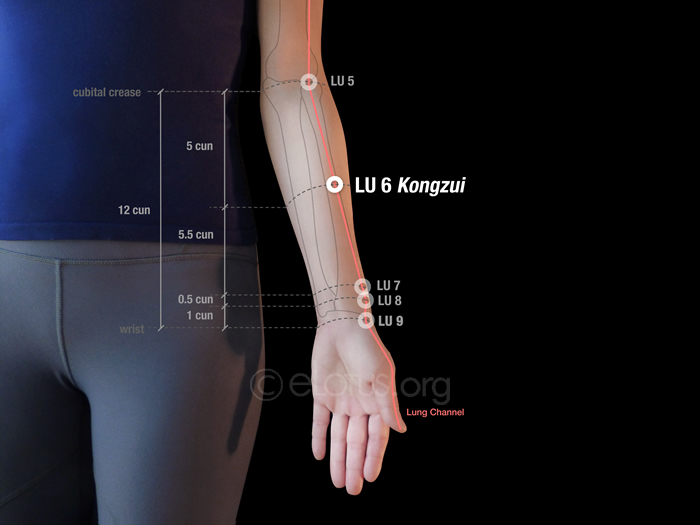
\includegraphics[width=\linewidth]{LU_6.jpg}\caption{Hình minh họa huyệt LU 6.}\end{figure}
\subsection*{Chỉ định}Ho, đau ngực, hen, ho ra máu, đau họng; đau co thắt khuỷu tay/cánh tay.
\subsection*{Ứng dụng}Điều hòa và giáng khí Phế; thanh nhiệt, chỉ huyết.
\subsection*{Thủ thuật}Châm thẳng 0{,}5--1 thốn.

\subsection{LU 7 - Liệt Khuyết (Lieque)}
\subsection*{Thông tin cơ bản}\begin{description}\item[Hán tự và phiên âm:] 列缺; liè quē.\item[Ý nghĩa tên:] Khe nứt (Broken Sequence).\item[Phân loại:] Huyệt Lạc của Phế; huyệt Xuất của kinh Phế; huyệt chủ Ren (Nhâm); huyệt chủ vùng đầu và gáy.\end{description}
\subsection*{Vị trí}Ở mặt quay cẳng tay, cách nếp gấp cổ tay 1{,}5 thốn về phía khuỷu, trong khe giữa gân cơ cánh tay quay và gân cơ dạng dài ngón cái. Có thể xác định bằng cách bắt chéo hai ngón trỏ và ngón cái; đầu ngón trỏ đặt tại mỏm trâm quay của bàn tay kia, huyệt ở chỗ lõm dưới đầu ngón trỏ.
\begin{figure}[H]\centering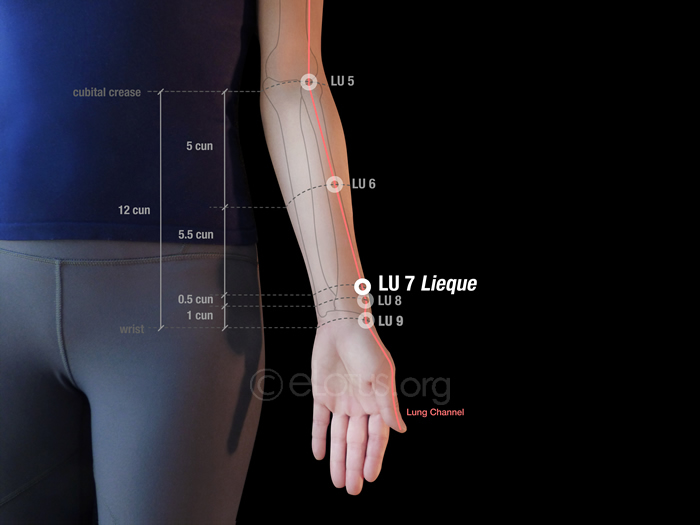
\includegraphics[width=\linewidth]{LU_7.jpg}\caption{Hình minh họa huyệt LU 7.}\end{figure}
\subsection*{Chỉ định}Ho, hen, đau họng; đau đầu, đau nửa đầu, cứng gáy; liệt mặt, đau răng; đau hoặc yếu cổ tay.
\subsection*{Ứng dụng}Giải biểu, khu phong; thông Phế, thúc đẩy chức năng túc giáng; khai mở và điều hòa mạch Nhâm; điều hòa thủy đạo; lợi đầu và cổ.
\subsection*{Thủ thuật}Châm xiên 0{,}3--0{,}5 thốn hướng lên khuỷu.

\subsection{LU 8 - Kinh Cừ (Jingqu)}
\subsection*{Thông tin cơ bản}\begin{description}\item[Hán tự và phiên âm:] 經渠; jīng qú.\item[Ý nghĩa tên:] Mương kinh (Channel Ditch, Channel Canal).\item[Phân loại:] Ngũ hành thuộc Kim; huyệt Kinh (Jing-River) thuộc Kim.\end{description}
\subsection*{Vị trí}Cách nếp gấp cổ tay 1 thốn về phía khuỷu, trong chỗ lõm bên ngoài động mạch quay.
\begin{figure}[H]\centering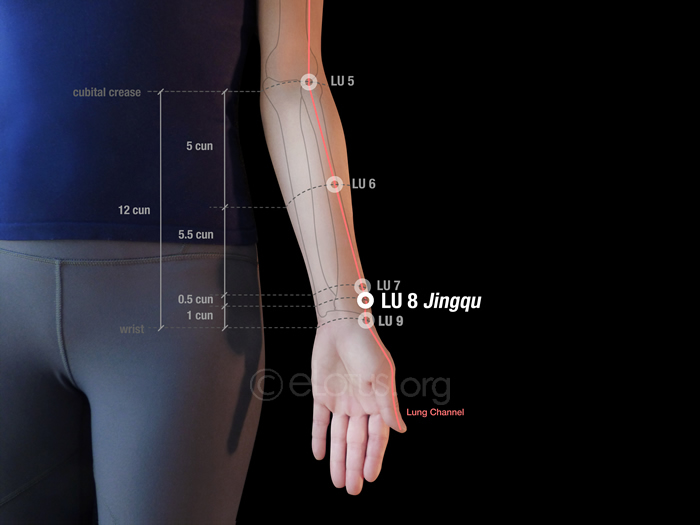
\includegraphics[width=\linewidth]{LU_8.jpg}\caption{Hình minh họa huyệt LU 8.}\end{figure}
\subsection*{Chỉ định}Ho, hen, khò khè; sốt, đau ngực, đau họng; đau cổ tay.
\subsection*{Ứng dụng}Giáng khí Phế.
\subsection*{Thủ thuật}Châm thẳng 0{,}1--0{,}3 thốn; tránh chọc vào động mạch quay.

\subsection{LU 9 - Thái Uyên (Taiyuan)}
\subsection*{Thông tin cơ bản}\begin{description}\item[Hán tự và phiên âm:] 太淵; tài yuān.\item[Ý nghĩa tên:] Vực lớn (Great Abyss, Greater Abyss).\item[Phân loại:] Ngũ hành thuộc Thổ; huyệt Du (Shu-Stream) thuộc Thổ; Nguyên huyệt của Phế; hội huyệt thứ 8, chủ về mạch máu.\end{description}
\subsection*{Vị trí}Ở đầu quay của nếp gấp cổ tay, trong chỗ lõm phía ngoài động mạch quay.
\begin{figure}[H]\centering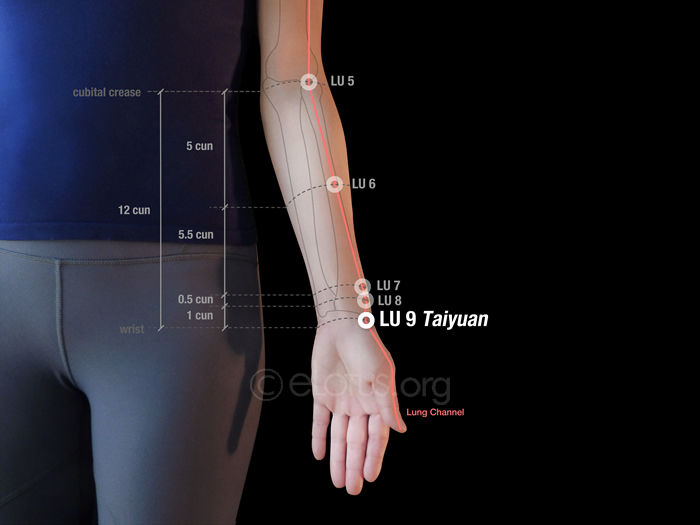
\includegraphics[width=\linewidth]{LU_9.jpg}\caption{Hình minh họa huyệt LU 9.}\end{figure}
\subsection*{Chỉ định}Ho mạn tính, ho yếu, khò khè, hen, ho ra máu, đau họng; hồi hộp; đau ngực, cổ tay hoặc cánh tay.
\subsection*{Ứng dụng}Bổ và điều hòa khí Phế; khu phong, hóa đàm; thông kinh, giảm đau.
\subsection*{Thủ thuật}Châm thẳng 0{,}2--0{,}3 thốn; tránh chọc vào động mạch quay.

\subsection{LU 10 - Ngư Tế (Yuji)}
\subsection*{Thông tin cơ bản}\begin{description}\item[Hán tự và phiên âm:] 魚際; yú jì.\item[Ý nghĩa tên:] Bờ cá (Fish Border).\item[Phân loại:] Ngũ hành thuộc Hỏa; huyệt Huỳnh (Ying-Spring) thuộc Hỏa.\end{description}
\subsection*{Vị trí}Ở chỗ tiếp giáp da đỏ và da trắng tại mô cái, trong chỗ lõm giữa xương bàn tay thứ nhất.
\begin{figure}[H]\centering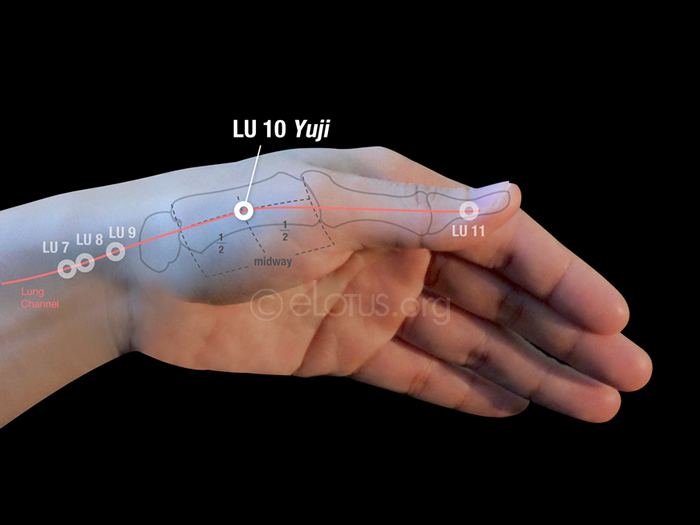
\includegraphics[width=\linewidth]{LU_10.jpg}\caption{Hình minh họa huyệt LU 10.}\end{figure}
\subsection*{Chỉ định}Ho, ho ra máu, đau họng, mất tiếng; sốt, nóng lòng bàn tay.
\subsection*{Ứng dụng}Thanh nhiệt Phế, giáng khí nghịch, lợi họng; điều hòa Vị và Tâm.
\subsection*{Thủ thuật}Châm thẳng 0{,}5--1 thốn.

\subsection{LU 11 - Thiếu Thương (Shaoshang)}
\subsection*{Thông tin cơ bản}\begin{description}\item[Hán tự và phiên âm:] 少商; shào shāng.\item[Ý nghĩa tên:] Thiếu Thương, kim loại non (Lesser Shang, Lesser Metal).\item[Phân loại:] Ngũ hành thuộc Mộc; huyệt Tỉnh (Jing-Well) thuộc Mộc; Quỷ huyệt thứ 13, tên Faith.\end{description}
\subsection*{Vị trí}Ở phía quay ngón cái, cách góc móng khoảng 0{,}1 thốn về phía sau.
\begin{figure}[H]\centering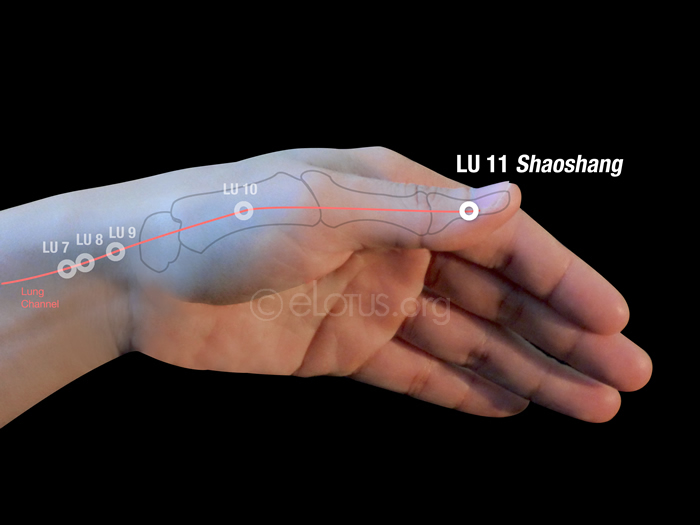
\includegraphics[width=\linewidth]{LU_11.jpg}\caption{Hình minh họa huyệt LU 11.}\end{figure}
\subsection*{Chỉ định}Đau họng, viêm amidan, ho, hen, chảy máu cam; sốt, mất ý thức, hưng cảm; đau co thắt ngón cái.
\subsection*{Ứng dụng}Thanh nhiệt, lợi họng; hồi tỉnh.
\subsection*{Thủ thuật}Châm xiên 0{,}1 thốn hoặc chích nặn máu.

\clearpage
\section{Kinh Túc Dương Minh Vị}
\begin{description}
\item[Tên kinh:] Túc Dương Minh Vị (Foot Yangming, Stomach Channel).
\item[Hán tự và phiên âm:] 足陽明胃經; zú yáng míng wèi jīng.
\item[Thời gian hoạt động:] 7--9 giờ sáng.
\item[Ngũ hành:] Thổ (Earth).
\item[Kinh biểu lý:] Túc Thái Âm Tỳ (Foot Taiyin, Spleen Channel).
\end{description}
\subsection*{Đường đi}
Kinh bắt đầu ở phía ngoài cánh mũi tại Nghinh Hương (LI 20), đi lên sống mũi đến Tình Minh (BL 1), rồi vòng xuống dọc bên mũi đến Thừa Khấp (ST 1), vào lợi hàm trên. Kinh xuất hiện lại tại Nhân Trung (GV 26), vòng quanh môi đến Thừa Tương (CV 24), chạy dọc bờ hàm dưới qua Đại Nghinh (ST 5), rồi lên trước tai đến Đầu Duy (ST 8), đi qua các huyệt thuộc kinh Đởm và đến Thần Đình (GV 24). Một nhánh từ Đại Nghinh đi xuống Nhân Nghinh (ST 9), dọc họng vào hõm thượng đòn, xuống qua Đại Chùy (GV 14), xuyên cơ hoành, qua Trung Quản (CV 12) và Thượng Quản (CV 13), vào Vị và liên hệ với Tỳ. Nhánh thẳng từ hõm thượng đòn đi xuống qua núm vú, qua rốn đến Khí Xung (ST 30). Nhánh từ môn vị đi xuống trong bụng và nhập với nhánh trên tại Khí Xung. Kinh tiếp tục xuống đến Lệ Đoài (ST 45); nhánh ở cẳng chân tách từ Túc Tam Lý (ST 36) đến ngón chân giữa; nhánh ở mu chân xuất phát từ Xung Dương (ST 42) đến mặt trong đầu ngón chân cái tại Ẩn Bạch (SP 1), nối với kinh Tỳ.
\subsection*{Chỉ định của kinh}
\begin{itemize}\item Sôi bụng, chướng bụng, đau vùng thượng vị, nôn, cảm giác đói.\item Méo miệng và mắt.\item Đau bụng và đau mặt ngoài chi dưới.\end{itemize}
\subsection*{Ứng dụng của kinh}
Tiếp nhận và phân giải thức ăn; kiểm soát quá trình làm chín và chuyển hóa thức ăn, vận chuyển tinh chất thức ăn, điều khiển sự giáng xuống của khí; là nguồn sinh tân dịch.
\subsection*{Phương pháp cân bằng}
\begin{enumerate}\item Thủ Dương Minh Đại Trường (Hand Yangming, Large Intestine).\item Thủ Quyết Âm Tâm Bào (Hand Jueyin, Pericardium).\item Túc Thái Âm Tỳ (Foot Taiyin, Spleen).\item Thủ Quyết Âm Tâm Bào (Hand Jueyin, Pericardium).\item Thủ Dương Minh Đại Trường (Hand Yangming, Large Intestine).\end{enumerate}
\subsection*{Phân loại huyệt đặc biệt trên kinh}
\begin{itemize}\item Ngũ Du: Tỉnh (Jing-Well) ST 45; Huỳnh (Ying-Spring) ST 44; Du (Shu-Stream) ST 43; Kinh (Jing-River) ST 41; Hợp (He-Sea) ST 36.\item Nguyên huyệt: Xung Dương (ST 42); Lạc huyệt: Phong Long (ST 40); Khích huyệt: Lương Khâu (ST 34).\item Mộ huyệt trước: Trung Quản (CV 12); Du huyệt sau: Vị Du (BL 21); Hạ Hợp huyệt: Túc Tam Lý (ST 36).\item Huyệt Mẹ: Giải Khê (ST 41); huyệt Con: Lệ Đoài (ST 45); huyệt Nhập: Thừa Khấp (ST 1); huyệt Xuất: Xung Dương (ST 42).\end{itemize}
\subsection{ST 1 - Thừa Khấp (Chengqi)}
\subsection*{Thông tin cơ bản}\begin{description}\item[Hán tự và phiên âm:] 承泣; chéng qì.\item[Ý nghĩa tên:] Vật chứa nước mắt (dịch sát nghĩa; literal translation); tiếng Anh nguồn: Tear Container.\end{description}
\subsection*{Vị trí}Mắt nhìn thẳng, ngay dưới đồng tử, giữa nhãn cầu và bờ dưới ổ mắt.
\begin{figure}[H]\centering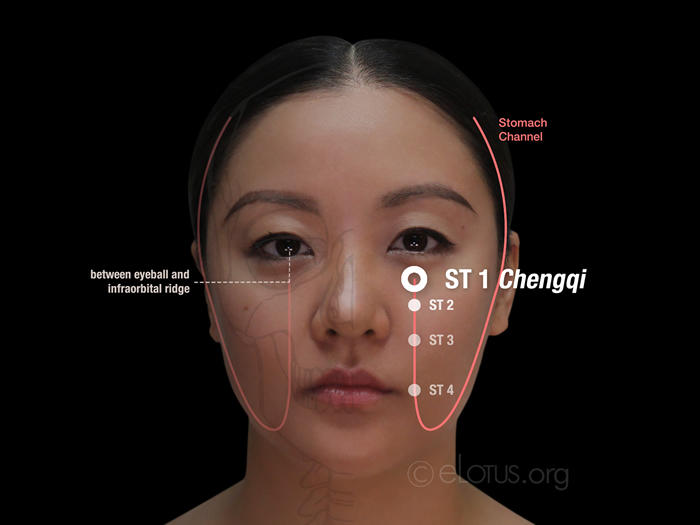
\includegraphics[width=\linewidth]{ST_1.jpg}\caption{Hình minh họa huyệt ST 1.}\end{figure}
\subsection*{Chỉ định}Đỏ, sưng, đau mắt; chảy nước mắt; quáng gà; co giật mi mắt; liệt mặt.
\subsection*{Ứng dụng}Lợi mắt; khu phong, thanh nhiệt.
\subsection*{Thủ thuật và lưu ý}Khi người bệnh nhắm mắt, đẩy nhãn cầu lên trên bằng ngón cái rồi châm thẳng, chậm 0,5--1 thốn dọc bờ dưới ổ mắt. Rút kim xong ép bông ít nhất một phút để tránh tụ máu. Không cứu và không vê, nâng, đẩy kim.

\subsection{ST 2 - Tứ Bạch (Sibai)}
\subsection*{Thông tin cơ bản}\begin{description}\item[Hán tự và phiên âm:] 四白; sì bái.\item[Ý nghĩa tên:] Bốn sắc trắng (dịch sát nghĩa; literal translation); tiếng Anh nguồn: Four Whites.\end{description}
\subsection*{Vị trí}Mắt nhìn thẳng, ngay dưới đồng tử, trong chỗ lõm tại lỗ dưới ổ mắt.
\begin{figure}[H]\centering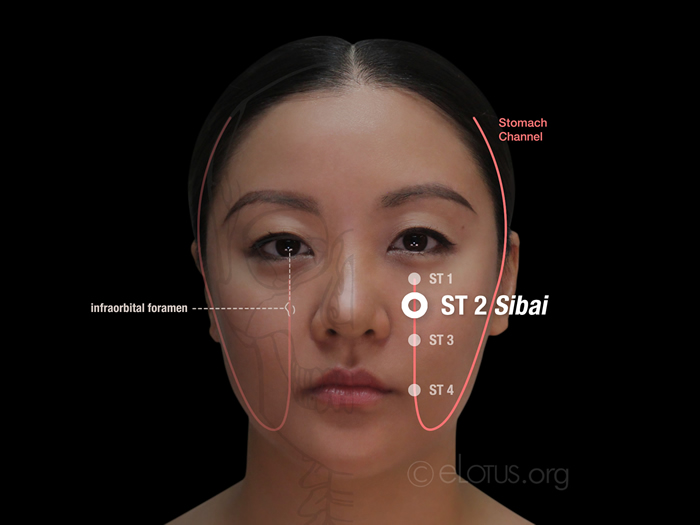
\includegraphics[width=\linewidth]{ST_2.jpg}\caption{Hình minh họa huyệt ST 2.}\end{figure}
\subsection*{Chỉ định}Đỏ, đau, ngứa mắt; co giật mi mắt; liệt mặt; đau mặt.
\subsection*{Ứng dụng}Khu phong, thanh nhiệt; lợi mắt.
\subsection*{Thủ thuật và lưu ý}Châm thẳng 0,2--0,3 thốn; không nên châm sâu. Không cứu và không thao tác nâng, đẩy, vê kim.

\subsection{ST 3 - Cự Liêu (Juliao)}
\subsection*{Thông tin cơ bản}\begin{description}\item[Hán tự và phiên âm:] 巨髎; jù liáo.\item[Ý nghĩa tên:] Hốc xương lớn (dịch sát nghĩa; literal translation); tiếng Anh nguồn: Great Bone Hole.\end{description}
\subsection*{Vị trí}Mắt nhìn thẳng, dưới đồng tử, ngang bờ dưới cánh mũi, phía ngoài rãnh mũi-má.
\begin{figure}[H]\centering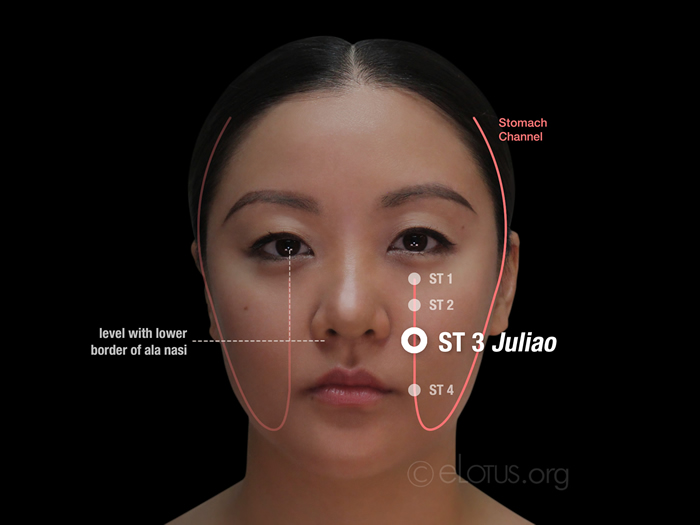
\includegraphics[width=\linewidth]{ST_3.jpg}\caption{Hình minh họa huyệt ST 3.}\end{figure}
\subsection*{Chỉ định}Liệt mặt, co giật mi mắt; chảy máu cam; đau răng; sưng môi và má.
\subsection*{Ứng dụng}Khu phong, tiêu sưng, giảm đau.
\subsection*{Thủ thuật và lưu ý}Châm thẳng 0,3--0,5 thốn.

\subsection{ST 4 - Địa Thương (Dicang)}
\subsection*{Thông tin cơ bản}\begin{description}\item[Hán tự và phiên âm:] 地倉; dì cāng.\item[Ý nghĩa tên:] Kho lương của Đất (dịch sát nghĩa; literal translation); tiếng Anh nguồn: Earth Granary.\end{description}
\subsection*{Vị trí}Mắt nhìn thẳng, ngay dưới đồng tử và phía ngoài khóe miệng; hoặc cách khóe miệng 0,4 thốn về phía ngoài.
\begin{figure}[H]\centering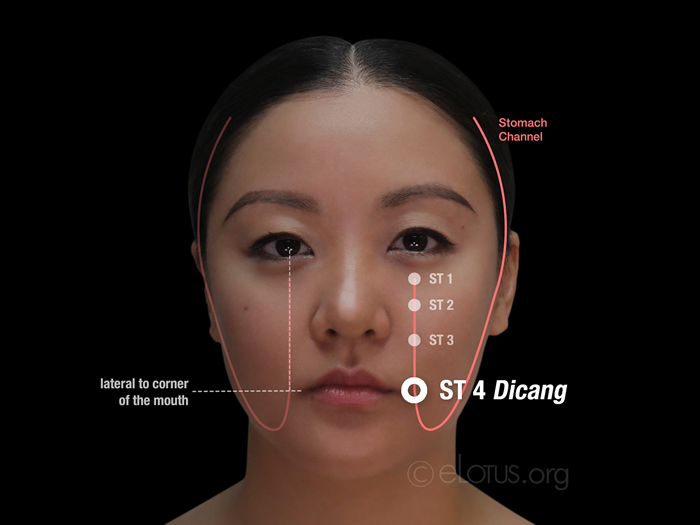
\includegraphics[width=\linewidth]{ST_4.jpg}\caption{Hình minh họa huyệt ST 4.}\end{figure}
\subsection*{Chỉ định}Méo miệng; co giật mi mắt; chảy dãi.
\subsection*{Ứng dụng}Khu phong vùng mặt; thông kinh, giảm đau.
\subsection*{Thủ thuật và lưu ý}Châm dưới da 1--1,5 thốn, hướng mũi kim về Giáp Xa (ST 6). Là huyệt hội của kinh Vị, Đại Trường, mạch Nhâm và mạch Dương Kiều.

\subsection{ST 5 - Đại Nghinh (Daying)}
\subsection*{Thông tin cơ bản}\begin{description}\item[Hán tự và phiên âm:] 大迎; dà yíng.\item[Ý nghĩa tên:] Sự tiếp đón lớn (dịch sát nghĩa; literal translation); tiếng Anh nguồn: Great Reception.\end{description}
\subsection*{Vị trí}Phía trước góc hàm dưới, trong chỗ lõm ở bờ trước cơ cắn; hõm rõ khi phồng má.
\begin{figure}[H]\centering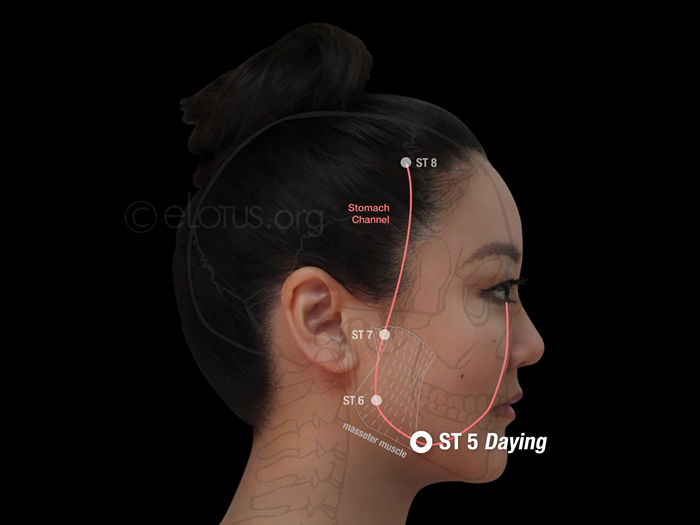
\includegraphics[width=\linewidth]{ST_5.jpg}\caption{Hình minh họa huyệt ST 5.}\end{figure}
\subsection*{Chỉ định}Liệt mặt, cứng hàm, sưng má; đau mặt, đau răng.
\subsection*{Ứng dụng}Khu phong, giảm sưng.
\subsection*{Thủ thuật và lưu ý}Châm xiên 0,3--0,5 thốn; tránh động mạch mặt.

\subsection{ST 6 - Giáp Xa (Jiache)}
\subsection*{Thông tin cơ bản}\begin{description}\item[Hán tự và phiên âm:] 頰車; jiá chē.\item[Ý nghĩa tên:] Xương hàm (dịch sát nghĩa; literal translation); tiếng Anh nguồn: Jaw Bone.\end{description}
\subsection*{Vị trí}Cách góc dưới xương hàm một khoát ngón tay về phía trước và phía trên, tại chỗ cơ cắn nổi lên khi nghiến răng.
\begin{figure}[H]\centering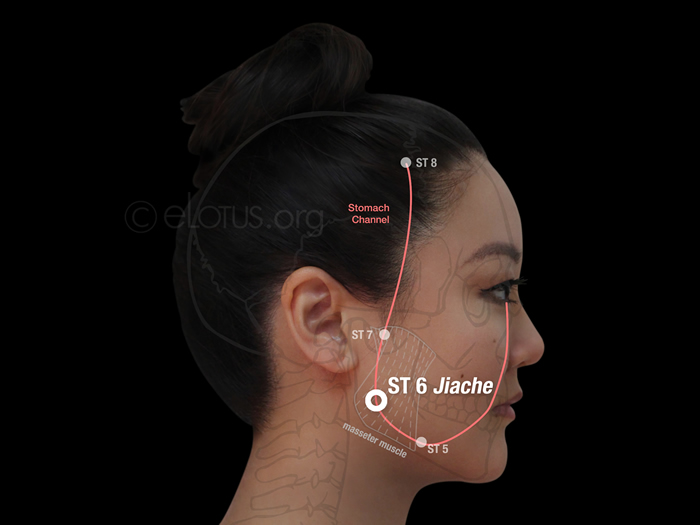
\includegraphics[width=\linewidth]{ST_6.jpg}\caption{Hình minh họa huyệt ST 6.}\end{figure}
\subsection*{Chỉ định}Liệt mặt, đau răng, sưng má và mặt, cứng hàm; quai bị.
\subsection*{Ứng dụng}Khu phong; lợi hàm và răng; thông kinh, giảm đau.
\subsection*{Thủ thuật và lưu ý}Châm thẳng 0,3--0,5 thốn hoặc châm dưới da hướng mũi kim về Địa Thương (ST 4). Có thể là Quỷ huyệt thứ 13, tên Bed.

\subsection{ST 7 - Hạ Quan (Xiaguan)}
\subsection*{Thông tin cơ bản}\begin{description}\item[Hán tự và phiên âm:] 下關; xià guān.\item[Ý nghĩa tên:] Phía dưới khớp (dịch sát nghĩa; literal translation); tiếng Anh nguồn: Below the Joint.\end{description}
\subsection*{Vị trí}Phía trước tai, ở bờ dưới cung gò má, trong hõm giữa cung gò má và khuyết hàm; xác định khi miệng ngậm.
\begin{figure}[H]\centering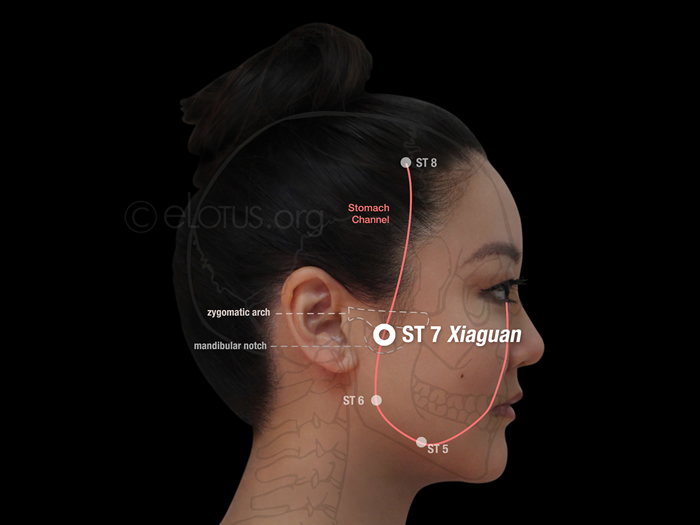
\includegraphics[width=\linewidth]{ST_7.jpg}\caption{Hình minh họa huyệt ST 7.}\end{figure}
\subsection*{Chỉ định}Điếc, ù tai, chảy dịch tai; đau răng; liệt mặt, đau mặt; rối loạn vận động hàm.
\subsection*{Ứng dụng}Lợi tai, hàm và răng; thông kinh, giảm đau.
\subsection*{Thủ thuật và lưu ý}Châm thẳng 0,3--0,5 thốn khi miệng ngậm. Huyệt hội của kinh Vị và Đởm.

\subsection{ST 8 - Đầu Duy (Touwei)}
\subsection*{Thông tin cơ bản}\begin{description}\item[Hán tự và phiên âm:] 頭維; tóu wéi.\item[Ý nghĩa tên:] Góc đầu (dịch sát nghĩa; literal translation); tiếng Anh nguồn: Head Corner, Head Support.\end{description}
\subsection*{Vị trí}Ở góc trán, cao hơn đường chân tóc trước 0,5 thốn và cách đường giữa đầu 4,5 thốn (hoặc cách Thần Đình GV 24).
\begin{figure}[H]\centering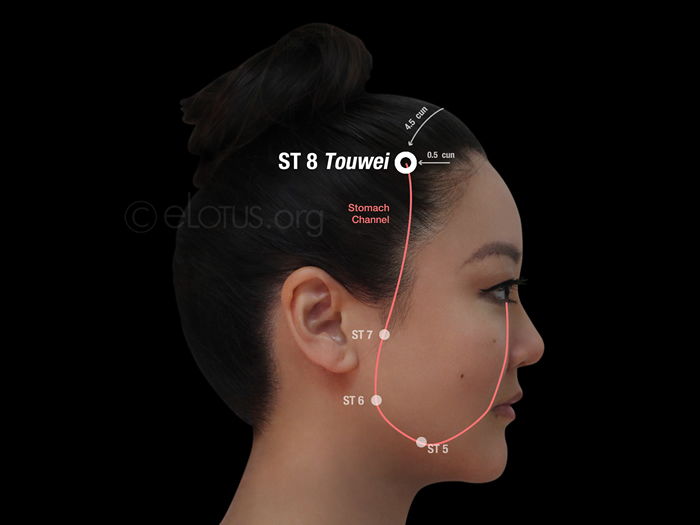
\includegraphics[width=\linewidth]{ST_8.jpg}\caption{Hình minh họa huyệt ST 8.}\end{figure}
\subsection*{Chỉ định}Đau đầu; nhìn mờ, đau mắt, chảy nước mắt.
\subsection*{Ứng dụng}Khu phong, giảm đau; lợi mắt.
\subsection*{Thủ thuật và lưu ý}Châm dưới da 0,5--1 thốn. Huyệt hội của kinh Vị, Đởm và mạch Dương Kiều.

\subsection{ST 9 - Nhân Nghinh (Renying)}
\subsection*{Thông tin cơ bản}\begin{description}\item[Hán tự và phiên âm:] 人迎; rén yíng.\item[Ý nghĩa tên:] Sự nghênh đón con người (dịch sát nghĩa; literal translation); tiếng Anh nguồn: Person's Welcome.\end{description}
\subsection*{Vị trí}Ngang đầu mút sụn giáp, ở bờ trước cơ ức-đòn-chũm, nơi sờ thấy mạch cảnh chung đập.
\begin{figure}[H]\centering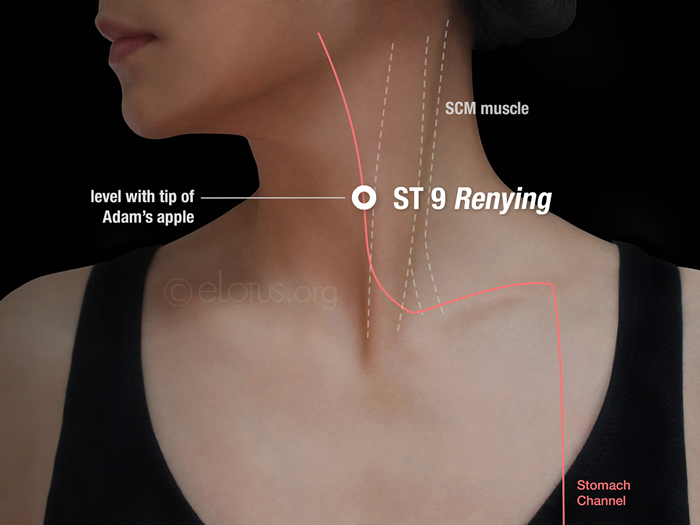
\includegraphics[width=\linewidth]{ST_9.jpg}\caption{Hình minh họa huyệt ST 9.}\end{figure}
\subsection*{Chỉ định}Đau, sưng họng; hen; bướu cổ; chóng mặt, đỏ bừng mặt.
\subsection*{Ứng dụng}Điều hòa khí huyết; lợi họng và cổ; giảm đau.
\subsection*{Thủ thuật và lưu ý}Châm thẳng 0,3--0,5 thốn; tránh chọc động mạch cảnh chung. Huyệt Tứ Hải, biển Khí; huyệt Thiên Song.

\subsection{ST 10 - Thủy Đột (Shuitu)}
\subsection*{Thông tin cơ bản}\begin{description}\item[Hán tự và phiên âm:] 水突; shǔi tū.\item[Ý nghĩa tên:] Chỗ nhô cao của nước (dịch sát nghĩa; literal translation); tiếng Anh nguồn: Water Prominence.\end{description}
\subsection*{Vị trí}Ở bờ trước cơ ức-đòn-chũm, tại trung điểm đường nối Nhân Nghinh (ST 9) và Khí Xá (ST 11).
\begin{figure}[H]\centering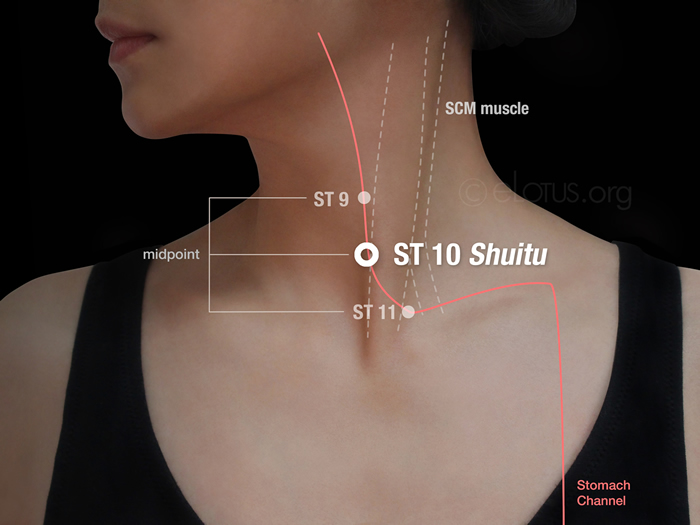
\includegraphics[width=\linewidth]{ST_10.jpg}\caption{Hình minh họa huyệt ST 10.}\end{figure}
\subsection*{Chỉ định}Đau họng, ho; hen.
\subsection*{Ứng dụng}Lợi họng và cổ; giáng khí Phế.
\subsection*{Thủ thuật và lưu ý}Châm thẳng 0,3--0,5 thốn.

\subsection{ST 11 - Khí Xá (Qishe)}
\subsection*{Thông tin cơ bản}\begin{description}\item[Hán tự và phiên âm:] 氣舍; qì shè.\item[Ý nghĩa tên:] Nơi cư ngụ của Khí (dịch sát nghĩa; literal translation); tiếng Anh nguồn: Qi Abode.\end{description}
\subsection*{Vị trí}Ở bờ trên đầu ức xương đòn, giữa đầu ức và đầu đòn cơ ức-đòn-chũm.
\begin{figure}[H]\centering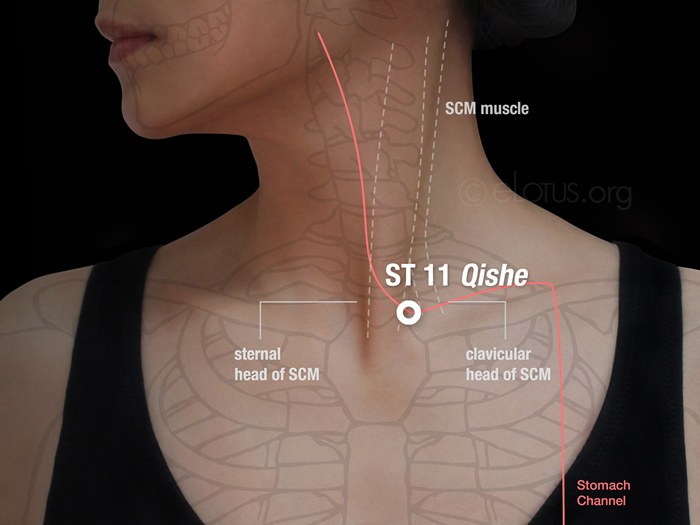
\includegraphics[width=\linewidth]{ST_11.jpg}\caption{Hình minh họa huyệt ST 11.}\end{figure}
\subsection*{Chỉ định}Đau họng; đau và cứng cổ; bướu cổ; hen; nấc.
\subsection*{Ứng dụng}Lợi họng và cổ; giáng khí.
\subsection*{Thủ thuật và lưu ý}Châm thẳng 0,3--0,5 thốn.

\subsection{ST 12 - Khuyết Bồn (Quepen)}
\subsection*{Thông tin cơ bản}\begin{description}\item[Hán tự và phiên âm:] 缺盆; quē pén.\item[Ý nghĩa tên:] Chậu rỗng (dịch sát nghĩa; literal translation); tiếng Anh nguồn: Empty Basin.\end{description}
\subsection*{Vị trí}Ở trung điểm hõm thượng đòn, cách đường giữa trước 4 thốn.
\begin{figure}[H]\centering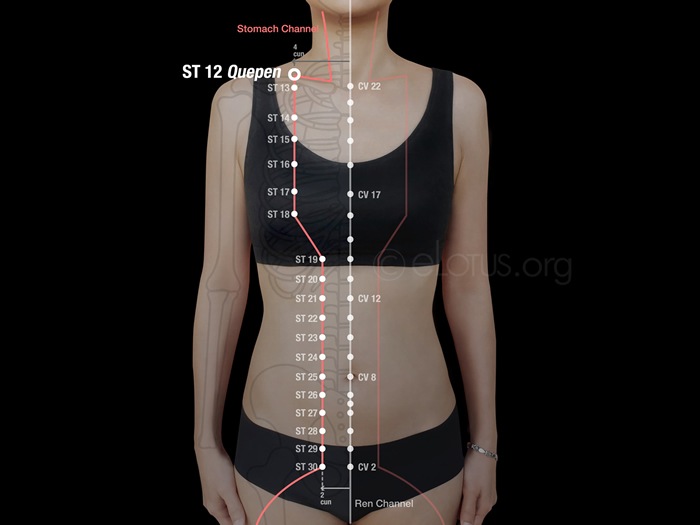
\includegraphics[width=\linewidth]{ST_12.jpg}\caption{Hình minh họa huyệt ST 12.}\end{figure}
\subsection*{Chỉ định}Ho, đau họng, hen; đau hõm thượng đòn.
\subsection*{Ứng dụng}Giáng khí Phế, thanh nhiệt ngực; thông kinh.
\subsection*{Thủ thuật và lưu ý}Không châm sâu vì có nguy cơ làm thủng phổi; nguồn ghi không khuyến nghị khi mang thai. Huyệt hội của các kinh Vị, Đại Trường, Tiểu Trường, Tam Tiêu và Đởm.

\subsection{ST 13 - Khí Hộ (Qihu)}
\subsection*{Thông tin cơ bản}\begin{description}\item[Hán tự và phiên âm:] 氣戶; qì hù.\item[Ý nghĩa tên:] Cửa Khí (dịch sát nghĩa; literal translation); tiếng Anh nguồn: Qi Door.\end{description}
\subsection*{Vị trí}Ngay dưới Khuyết Bồn (ST 12), ở bờ dưới xương đòn, cách đường giữa trước 4 thốn.
\begin{figure}[H]\centering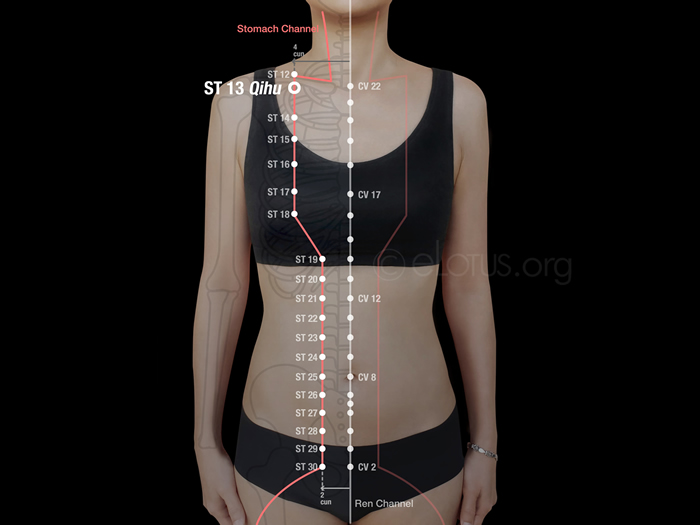
\includegraphics[width=\linewidth]{ST_13.jpg}\caption{Hình minh họa huyệt ST 13.}\end{figure}
\subsection*{Chỉ định}Đầy ngực, hen, ho, nấc; đau ngực và hạ sườn.
\subsection*{Ứng dụng}Giáng khí nghịch; giải uất vùng ngực.
\subsection*{Thủ thuật và lưu ý}Châm xiên 0,3--0,5 thốn; tránh châm sâu hoặc thẳng vì nguy cơ làm thủng phổi.

\subsection{ST 14 - Khố Phòng (Kufang)}
\subsection*{Thông tin cơ bản}\begin{description}\item[Hán tự và phiên âm:] 庫房; kù fáng.\item[Ý nghĩa tên:] Kho chứa (dịch sát nghĩa; literal translation); tiếng Anh nguồn: Storeroom.\end{description}
\subsection*{Vị trí}Khoang liên sườn thứ nhất, cách đường giữa trước 4 thốn về phía ngoài.
\begin{figure}[H]\centering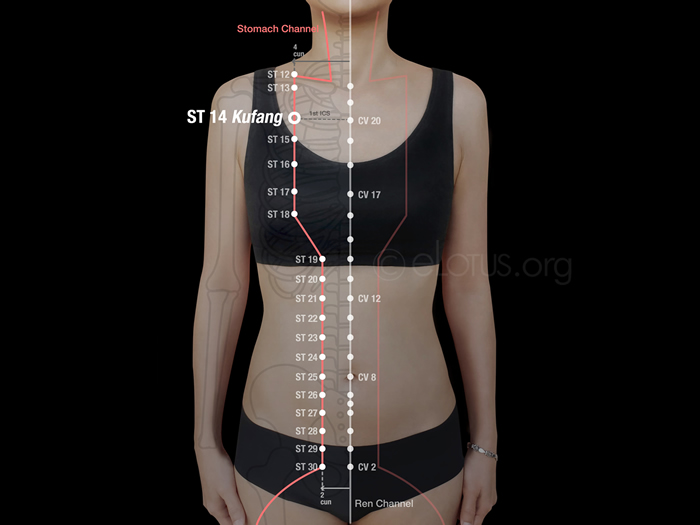
\includegraphics[width=\linewidth]{ST_14.jpg}\caption{Hình minh họa huyệt ST 14.}\end{figure}
\subsection*{Chỉ định}Đầy và đau ngực; ho.
\subsection*{Ứng dụng}Giáng khí nghịch; giải uất ngực.
\subsection*{Thủ thuật và lưu ý}Châm xiên 0,3--0,5 thốn; tránh châm sâu hoặc thẳng vì nguy cơ làm thủng phổi.

\subsection{ST 15 - Ốc Ế (Wuyi)}
\subsection*{Thông tin cơ bản}\begin{description}\item[Hán tự và phiên âm:] 屋翳; wū yì.\item[Ý nghĩa tên:] Mái nhà; bình phong (dịch sát nghĩa; literal translation); tiếng Anh nguồn: Roof, Room Screen.\end{description}
\subsection*{Vị trí}Khoang liên sườn thứ hai, cách đường giữa trước 4 thốn về phía ngoài.
\begin{figure}[H]\centering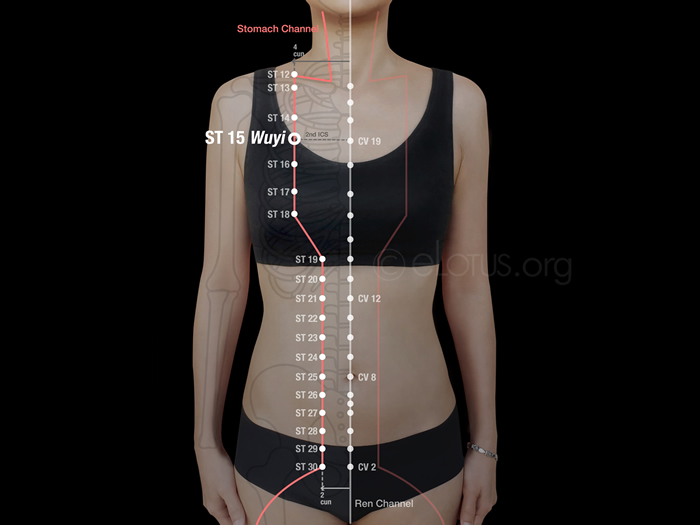
\includegraphics[width=\linewidth]{ST_15.jpg}\caption{Hình minh họa huyệt ST 15.}\end{figure}
\subsection*{Chỉ định}Đầy, đau ngực và vùng sườn; ho, hen; viêm tuyến vú.
\subsection*{Ứng dụng}Giáng khí nghịch, giải uất ngực; lợi vú và da.
\subsection*{Thủ thuật và lưu ý}Châm xiên 0,3--0,5 thốn; tránh châm sâu hoặc thẳng vì nguy cơ làm thủng phổi.

\subsection{ST 16 - Ưng Song (Yingchuang)}
\subsection*{Thông tin cơ bản}\begin{description}\item[Hán tự và phiên âm:] 膺窗; yìng chuāng.\item[Ý nghĩa tên:] Cửa sổ ngực (dịch sát nghĩa; literal translation); tiếng Anh nguồn: Breast Window.\end{description}
\subsection*{Vị trí}Khoang liên sườn thứ ba, cách đường giữa trước 4 thốn về phía ngoài.
\begin{figure}[H]\centering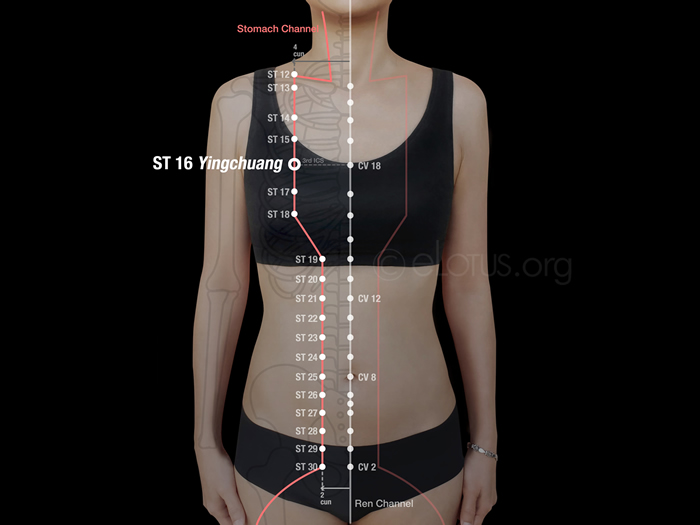
\includegraphics[width=\linewidth]{ST_16.jpg}\caption{Hình minh họa huyệt ST 16.}\end{figure}
\subsection*{Chỉ định}Đầy, đau ngực và hạ sườn; ho, hen; viêm tuyến vú.
\subsection*{Ứng dụng}Giáng khí nghịch; lợi vú và ngực.
\subsection*{Thủ thuật và lưu ý}Châm xiên 0,3--0,5 thốn; tránh châm sâu hoặc thẳng vì nguy cơ làm thủng phổi.

\subsection{ST 17 - Nhũ Trung (Ruzhong)}
\subsection*{Thông tin cơ bản}\begin{description}\item[Hán tự và phiên âm:] 乳中; rǔ zhōng.\item[Ý nghĩa tên:] Trung tâm ngực (dịch sát nghĩa; literal translation); tiếng Anh nguồn: Breast Center.\end{description}
\subsection*{Vị trí}Ở chính giữa núm vú, khoang liên sườn thứ tư, cách đường giữa trước 4 thốn.
\begin{figure}[H]\centering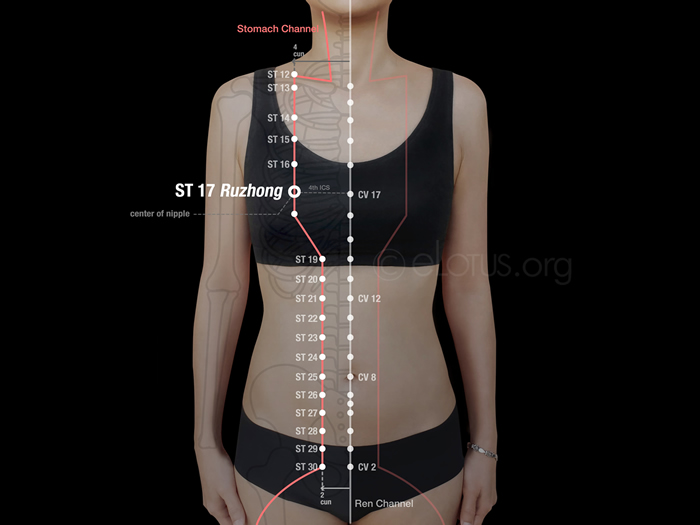
\includegraphics[width=\linewidth]{ST_17.jpg}\caption{Hình minh họa huyệt ST 17.}\end{figure}
\subsection*{Chỉ định}Không có chỉ định.
\subsection*{Ứng dụng}Không nêu ứng dụng.
\subsection*{Thủ thuật và lưu ý}Không châm, không cứu; chỉ dùng làm mốc định vị huyệt trên ngực và bụng.

\subsection{ST 18 - Nhũ Căn (Rugen)}
\subsection*{Thông tin cơ bản}\begin{description}\item[Hán tự và phiên âm:] 乳根; rǔ gēn.\item[Ý nghĩa tên:] Gốc ngực (dịch sát nghĩa; literal translation); tiếng Anh nguồn: Breast Root.\end{description}
\subsection*{Vị trí}Khoang liên sườn thứ năm, cách đường giữa trước 4 thốn; ngay dưới núm vú, ở bờ dưới vú.
\begin{figure}[H]\centering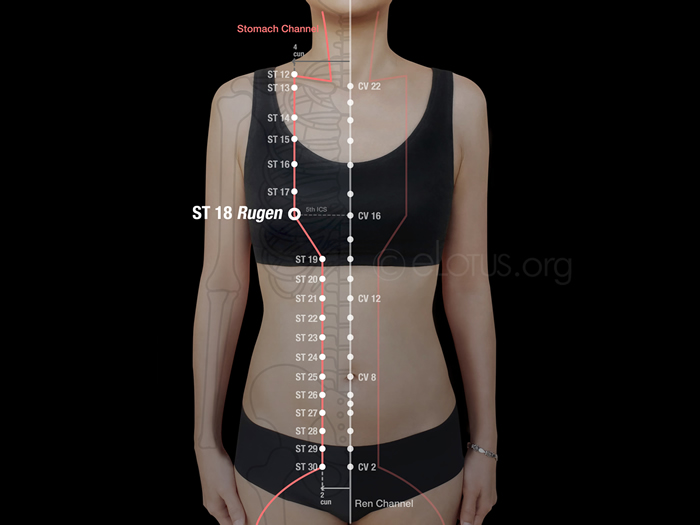
\includegraphics[width=\linewidth]{ST_18.jpg}\caption{Hình minh họa huyệt ST 18.}\end{figure}
\subsection*{Chỉ định}Viêm tuyến vú, ít sữa; đau ngực, ho, hen.
\subsection*{Ứng dụng}Lợi vú, giảm sưng; giải ứ, thông ngực.
\subsection*{Thủ thuật và lưu ý}Châm xiên 0,3--0,5 thốn; tránh châm sâu hoặc thẳng vì nguy cơ làm thủng phổi.

\subsection{ST 19 - Bất Dung (Burong)}
\subsection*{Thông tin cơ bản}\begin{description}\item[Hán tự và phiên âm:] 不容; bù róng.\item[Ý nghĩa tên:] Không dung chứa (dịch sát nghĩa; literal translation); tiếng Anh nguồn: Not Contained.\end{description}
\subsection*{Vị trí}Cách rốn 6 thốn phía trên, cách đường giữa trước 2 thốn, ngang Cự Khuyết (CV 14).
\begin{figure}[H]\centering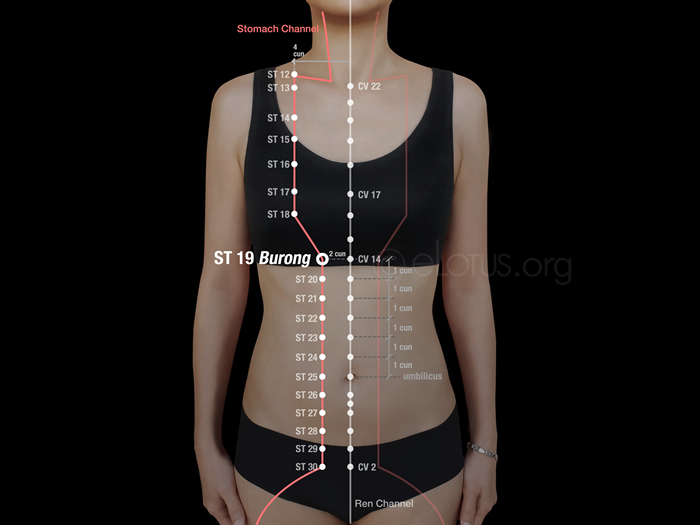
\includegraphics[width=\linewidth]{ST_19.jpg}\caption{Hình minh họa huyệt ST 19.}\end{figure}
\subsection*{Chỉ định}Chướng bụng, nôn, đau dạ dày; chán ăn.
\subsection*{Ứng dụng}Điều hòa trung tiêu; giáng khí.
\subsection*{Thủ thuật và lưu ý}Châm thẳng 0,5--0,8 thốn.

\subsection{ST 20 - Thừa Mãn (Chengman)}
\subsection*{Thông tin cơ bản}\begin{description}\item[Hán tự và phiên âm:] 承滿; chéng mǎn.\item[Ý nghĩa tên:] Tiếp nhận sự đầy đủ (dịch sát nghĩa; literal translation); tiếng Anh nguồn: Assuming Fullness.\end{description}
\subsection*{Vị trí}Cách rốn 5 thốn phía trên, cách đường giữa trước 2 thốn, ngang Thượng Quản (CV 13).
\begin{figure}[H]\centering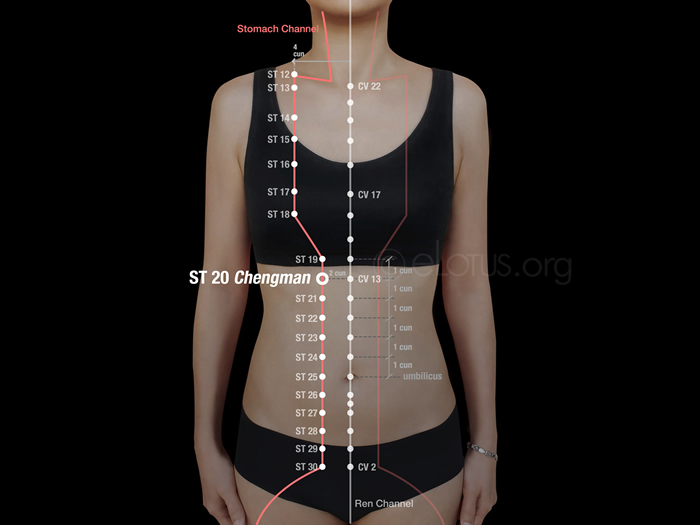
\includegraphics[width=\linewidth]{ST_20.jpg}\caption{Hình minh họa huyệt ST 20.}\end{figure}
\subsection*{Chỉ định}Đau dạ dày, chướng bụng, nôn; chán ăn.
\subsection*{Ứng dụng}Điều hòa trung tiêu; giáng khí nghịch của Phế và Vị.
\subsection*{Thủ thuật và lưu ý}Châm thẳng 0,5--1 thốn.

\subsection{ST 21 - Lương Môn (Liangmen)}
\subsection*{Thông tin cơ bản}\begin{description}\item[Hán tự và phiên âm:] 梁門; liáng mén.\item[Ý nghĩa tên:] Cửa xà ngang (dịch sát nghĩa; literal translation); tiếng Anh nguồn: Beam Gate.\end{description}
\subsection*{Vị trí}Cách rốn 4 thốn phía trên, cách đường giữa trước 2 thốn, ngang Trung Quản (CV 12).
\begin{figure}[H]\centering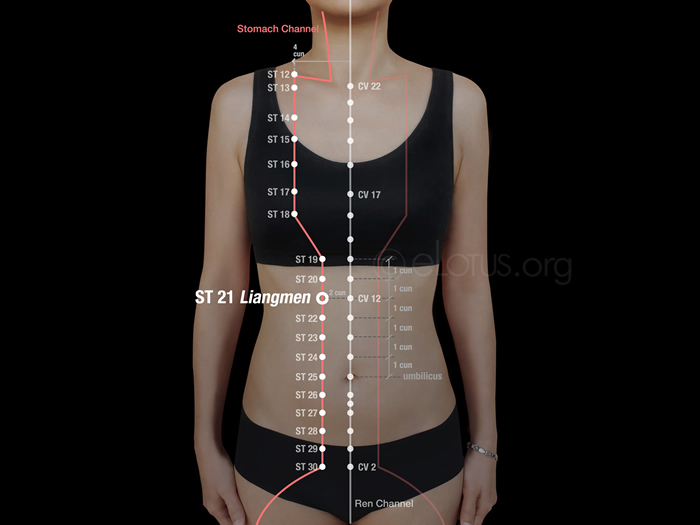
\includegraphics[width=\linewidth]{ST_21.jpg}\caption{Hình minh họa huyệt ST 21.}\end{figure}
\subsection*{Chỉ định}Nôn, chán ăn, tiêu chảy; đau dạ dày, chướng bụng.
\subsection*{Ứng dụng}Điều khí, giảm đau, thăng khí; điều hòa trung tiêu, hóa trệ.
\subsection*{Thủ thuật và lưu ý}Châm thẳng 0,8--1 thốn.

\subsection{ST 22 - Quan Môn (Guanmen)}
\subsection*{Thông tin cơ bản}\begin{description}\item[Hán tự và phiên âm:] 關門; guān mén.\item[Ý nghĩa tên:] Cửa ải (dịch sát nghĩa; literal translation); tiếng Anh nguồn: Pass Gate.\end{description}
\subsection*{Vị trí}Cách rốn 3 thốn phía trên, cách đường giữa trước 2 thốn, ngang Kiến Lý (CV 11).
\begin{figure}[H]\centering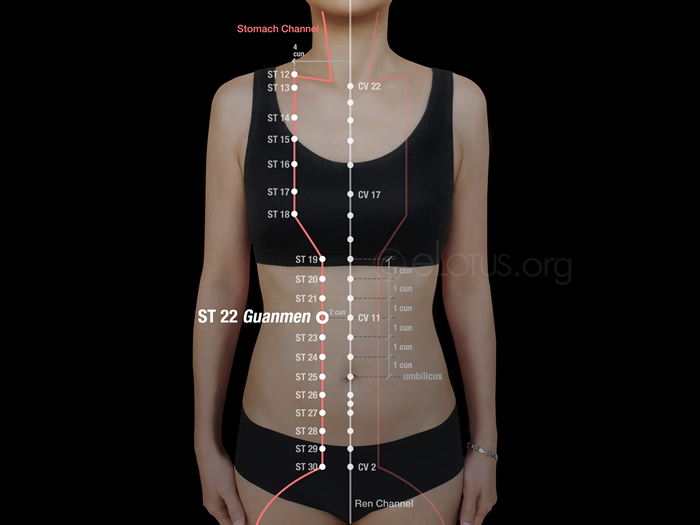
\includegraphics[width=\linewidth]{ST_22.jpg}\caption{Hình minh họa huyệt ST 22.}\end{figure}
\subsection*{Chỉ định}Chướng và đau bụng, chán ăn, sôi bụng; tiêu chảy, phù.
\subsection*{Ứng dụng}Điều khí, giảm đau; điều hòa ruột, lợi tiểu.
\subsection*{Thủ thuật và lưu ý}Châm thẳng 0,8--1 thốn.

\subsection{ST 23 - Thái Ất (Taiyi)}
\subsection*{Thông tin cơ bản}\begin{description}\item[Hán tự và phiên âm:] 太乙; tài yǐ.\item[Ý nghĩa tên:] Nhất thể tối cao (dịch sát nghĩa; literal translation); tiếng Anh nguồn: Supreme Unity.\end{description}
\subsection*{Vị trí}Cách rốn 2 thốn phía trên, cách đường giữa trước 2 thốn, ngang Hạ Quản (CV 10).
\begin{figure}[H]\centering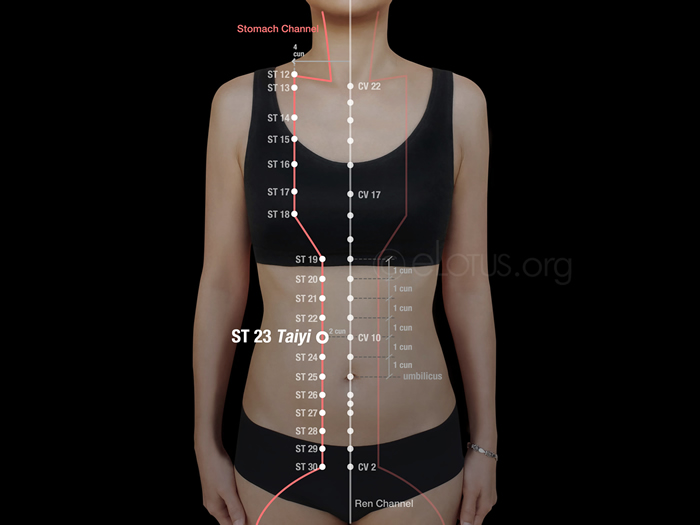
\includegraphics[width=\linewidth]{ST_23.jpg}\caption{Hình minh họa huyệt ST 23.}\end{figure}
\subsection*{Chỉ định}Đau dạ dày, khó tiêu; dễ kích động, hưng cảm.
\subsection*{Ứng dụng}Điều hòa trung tiêu; hóa đàm, an thần.
\subsection*{Thủ thuật và lưu ý}Châm thẳng 0,7--1 thốn.

\subsection{ST 24 - Hoạt Nhục Môn (Huaroumen)}
\subsection*{Thông tin cơ bản}\begin{description}\item[Hán tự và phiên âm:] 滑肉門; huá ròu mén.\item[Ý nghĩa tên:] Cửa thịt trơn (dịch sát nghĩa; literal translation); tiếng Anh nguồn: Slippery Flesh Gate.\end{description}
\subsection*{Vị trí}Cách rốn 1 thốn phía trên, cách đường giữa trước 2 thốn, ngang Thủy Phân (CV 9).
\begin{figure}[H]\centering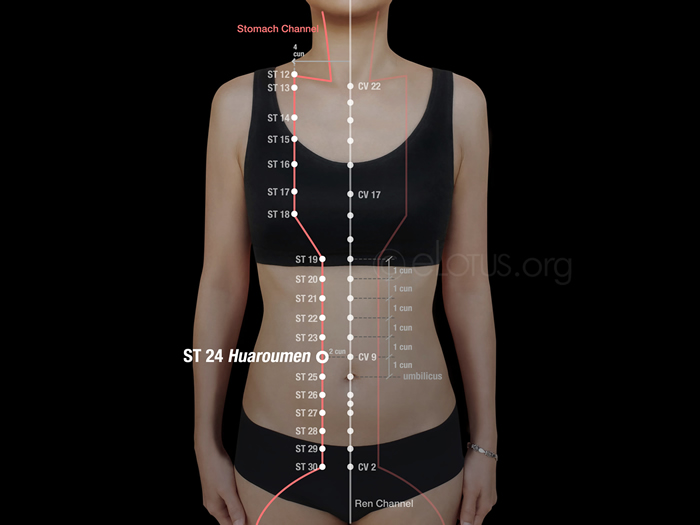
\includegraphics[width=\linewidth]{ST_24.jpg}\caption{Hình minh họa huyệt ST 24.}\end{figure}
\subsection*{Chỉ định}Đau dạ dày, nôn; hưng cảm.
\subsection*{Ứng dụng}Điều hòa Vị; hóa đàm, an thần.
\subsection*{Thủ thuật và lưu ý}Châm thẳng 0,7--1 thốn.

\subsection{ST 25 - Thiên Khu (Tianshu)}
\subsection*{Thông tin cơ bản}\begin{description}\item[Hán tự và phiên âm:] 天樞; tiān shū.\item[Ý nghĩa tên:] Trục trời (dịch sát nghĩa; literal translation); tiếng Anh nguồn: Celestial Pivot.\end{description}
\subsection*{Vị trí}Cách trung tâm rốn 2 thốn về hai bên.
\begin{figure}[H]\centering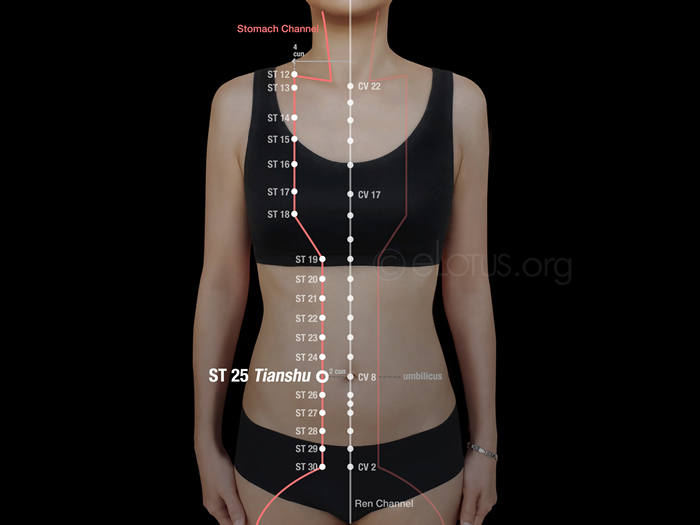
\includegraphics[width=\linewidth]{ST_25.jpg}\caption{Hình minh họa huyệt ST 25.}\end{figure}
\subsection*{Chỉ định}Đau, chướng bụng, sôi bụng, đau quanh rốn, phù; táo bón, tiêu chảy, lỵ; kinh nguyệt không đều.
\subsection*{Ứng dụng}Điều hòa ruột; điều hòa Tỳ Vị; hóa thấp và thấp nhiệt; điều hòa khí huyết, tiêu ứ.
\subsection*{Thủ thuật và lưu ý}Châm thẳng 0,7--1,2 thốn. Mộ huyệt trước của Đại Trường.

\subsection{ST 26 - Ngoại Lăng (Wailing)}
\subsection*{Thông tin cơ bản}\begin{description}\item[Hán tự và phiên âm:] 外陵; wài líng.\item[Ý nghĩa tên:] Gò ngoài (dịch sát nghĩa; literal translation); tiếng Anh nguồn: Outer Mound.\end{description}
\subsection*{Vị trí}Cách rốn 1 thốn phía dưới, cách đường giữa trước 2 thốn, ngang Âm Giao (CV 7).
\begin{figure}[H]\centering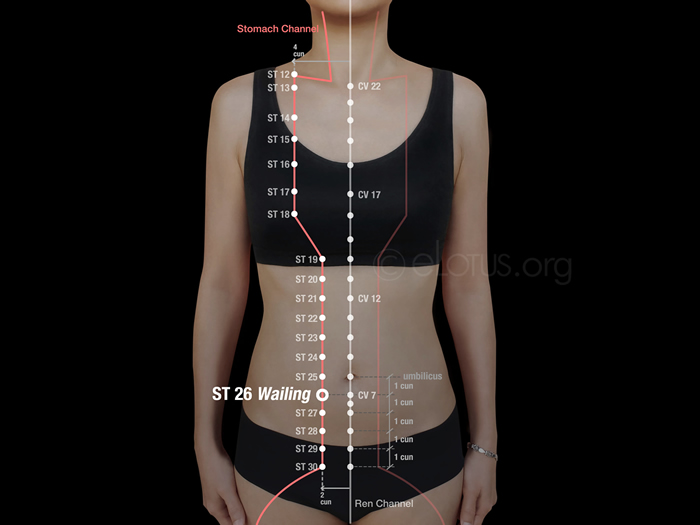
\includegraphics[width=\linewidth]{ST_26.jpg}\caption{Hình minh họa huyệt ST 26.}\end{figure}
\subsection*{Chỉ định}Đau bụng; thoát vị; thống kinh.
\subsection*{Ứng dụng}Điều khí, giảm đau.
\subsection*{Thủ thuật và lưu ý}Châm thẳng 0,7--1,2 thốn.

\subsection{ST 27 - Đại Cự (Daju)}
\subsection*{Thông tin cơ bản}\begin{description}\item[Hán tự và phiên âm:] 大巨; dà jù.\item[Ý nghĩa tên:] Lớn lao (dịch sát nghĩa; literal translation); tiếng Anh nguồn: Great Gigantic.\end{description}
\subsection*{Vị trí}Cách rốn 2 thốn phía dưới, cách đường giữa trước 2 thốn, ngang Thạch Môn (CV 5).
\begin{figure}[H]\centering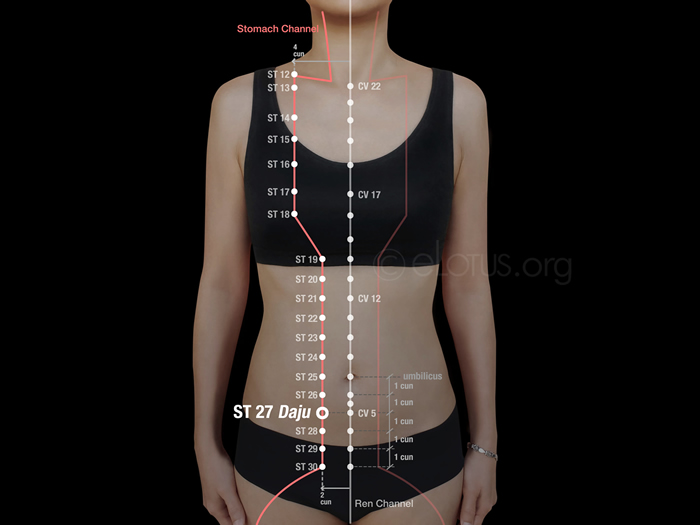
\includegraphics[width=\linewidth]{ST_27.jpg}\caption{Hình minh họa huyệt ST 27.}\end{figure}
\subsection*{Chỉ định}Chướng bụng dưới, tiểu khó, thoát vị; di tinh, xuất tinh sớm.
\subsection*{Ứng dụng}Bổ Thận, cố tinh; điều khí vùng bụng.
\subsection*{Thủ thuật và lưu ý}Châm thẳng 0,7--1,2 thốn.

\subsection{ST 28 - Thủy Đạo (Shuidao)}
\subsection*{Thông tin cơ bản}\begin{description}\item[Hán tự và phiên âm:] 水道; shuǐ dào.\item[Ý nghĩa tên:] Đường nước (dịch sát nghĩa; literal translation); tiếng Anh nguồn: Waterway.\end{description}
\subsection*{Vị trí}Cách rốn 3 thốn phía dưới, cách đường giữa trước 2 thốn, ngang Quan Nguyên (CV 4).
\begin{figure}[H]\centering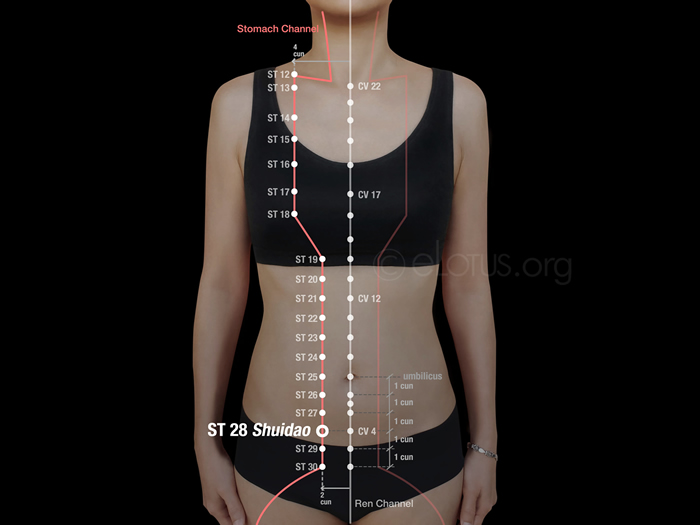
\includegraphics[width=\linewidth]{ST_28.jpg}\caption{Hình minh họa huyệt ST 28.}\end{figure}
\subsection*{Chỉ định}Chướng bụng dưới, bí tiểu, phù, thoát vị; thống kinh, vô sinh.
\subsection*{Ứng dụng}Điều hòa hạ tiêu, tiêu ứ; lợi Bàng Quang và tử cung.
\subsection*{Thủ thuật và lưu ý}Châm thẳng 0,7--1,2 thốn.

\subsection{ST 29 - Quy Lai (Guilai)}
\subsection*{Thông tin cơ bản}\begin{description}\item[Hán tự và phiên âm:] 歸來; guī lái.\item[Ý nghĩa tên:] Trở về (dịch sát nghĩa; literal translation); tiếng Anh nguồn: Return.\end{description}
\subsection*{Vị trí}Cách rốn 4 thốn phía dưới, cách đường giữa trước 2 thốn, ngang Trung Cực (CV 3).
\begin{figure}[H]\centering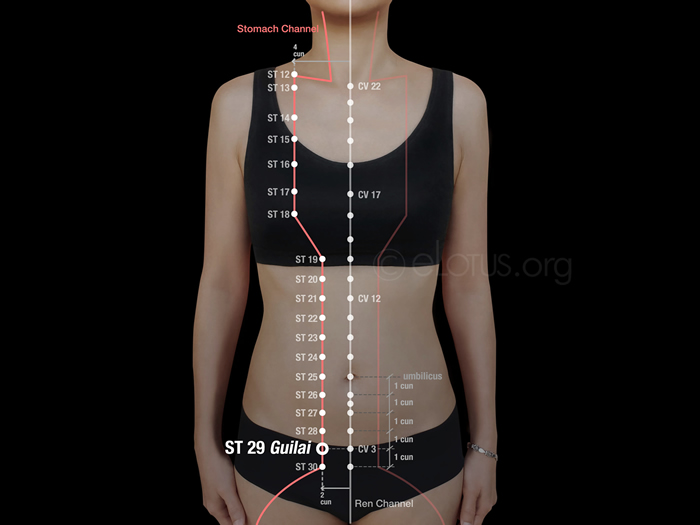
\includegraphics[width=\linewidth]{ST_29.jpg}\caption{Hình minh họa huyệt ST 29.}\end{figure}
\subsection*{Chỉ định}Đau bụng, thoát vị; thống kinh, kinh nguyệt không đều, vô kinh, khí hư, sa tử cung.
\subsection*{Ứng dụng}Ôn hạ tiêu và tử cung; điều kinh, lợi vùng sinh dục.
\subsection*{Thủ thuật và lưu ý}Châm thẳng 0,7--1,2 thốn.

\subsection{ST 30 - Khí Xung (Qichong)}
\subsection*{Thông tin cơ bản}\begin{description}\item[Hán tự và phiên âm:] 氣沖; qì chōng.\item[Ý nghĩa tên:] Khí xung (dịch sát nghĩa; literal translation); tiếng Anh nguồn: Surging Qi.\end{description}
\subsection*{Vị trí}Cách rốn 5 thốn phía dưới, cách đường giữa trước 2 thốn, ngang Khúc Cốt (CV 2).
\begin{figure}[H]\centering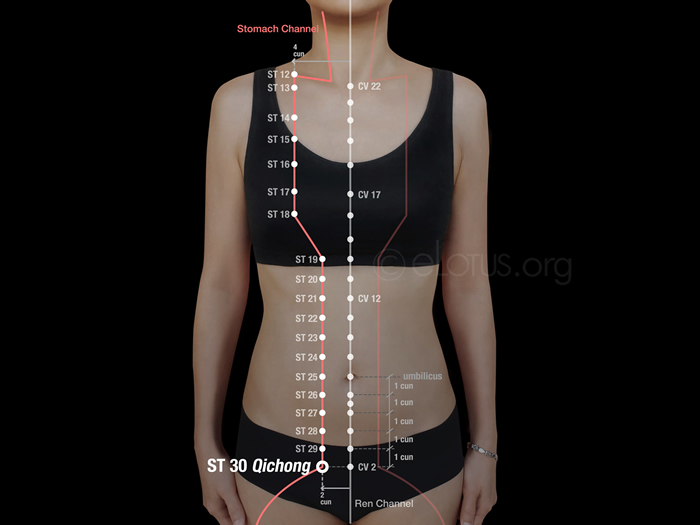
\includegraphics[width=\linewidth]{ST_30.jpg}\caption{Hình minh họa huyệt ST 30.}\end{figure}
\subsection*{Chỉ định}Đau bụng, sôi bụng, thoát vị; sưng đau cơ quan sinh dục ngoài, liệt dương; thống kinh, kinh nguyệt không đều.
\subsection*{Ứng dụng}Điều khí hạ tiêu; điều hòa mạch Xung; giáng khí bôn đồn.
\subsection*{Thủ thuật và lưu ý}Châm thẳng 0,5--1 thốn. Huyệt Tứ Hải, biển Dinh dưỡng.

\subsection{ST 31 - Bễ Quan (Biguan)}
\subsection*{Thông tin cơ bản}\begin{description}\item[Hán tự và phiên âm:] 髀關; bì guān.\item[Ý nghĩa tên:] Khớp đùi (dịch sát nghĩa; literal translation); tiếng Anh nguồn: Thigh Joint.\end{description}
\subsection*{Vị trí}Ở mặt trước đùi, trong hõm ngoài cơ may, trên đường nối gai chậu trước trên với góc trên-ngoài xương bánh chè, ngang bờ dưới khớp mu.
\begin{figure}[H]\centering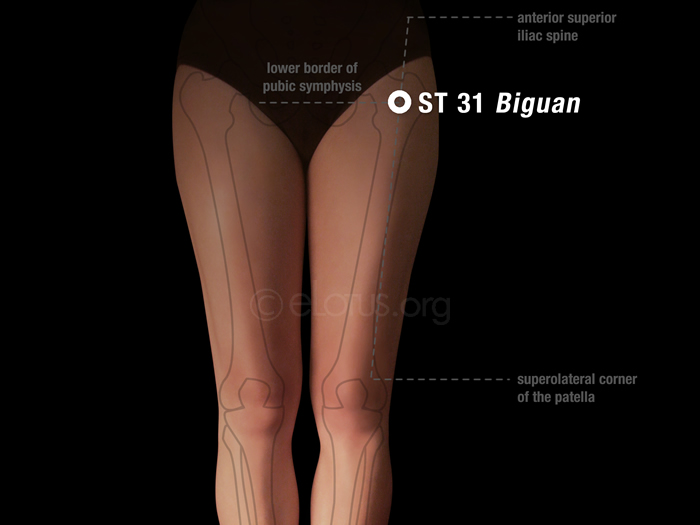
\includegraphics[width=\linewidth]{ST_31.jpg}\caption{Hình minh họa huyệt ST 31.}\end{figure}
\subsection*{Chỉ định}Đau đùi, teo cơ, hạn chế vận động, tê và đau chi dưới.
\subsection*{Ứng dụng}Thông kinh, giảm đau; khu phong thấp.
\subsection*{Thủ thuật và lưu ý}Châm thẳng 0,7--1 thốn.

\subsection{ST 32 - Phục Thỏ (Futu)}
\subsection*{Thông tin cơ bản}\begin{description}\item[Hán tự và phiên âm:] 伏兔; fú tù.\item[Ý nghĩa tên:] Thỏ phục (dịch sát nghĩa; literal translation); tiếng Anh nguồn: Crouching Rabbit.\end{description}
\subsection*{Vị trí}Trên đường nối gai chậu trước trên với bờ ngoài xương bánh chè, cách góc trên-ngoài bánh chè 6 thốn về phía trên.
\begin{figure}[H]\centering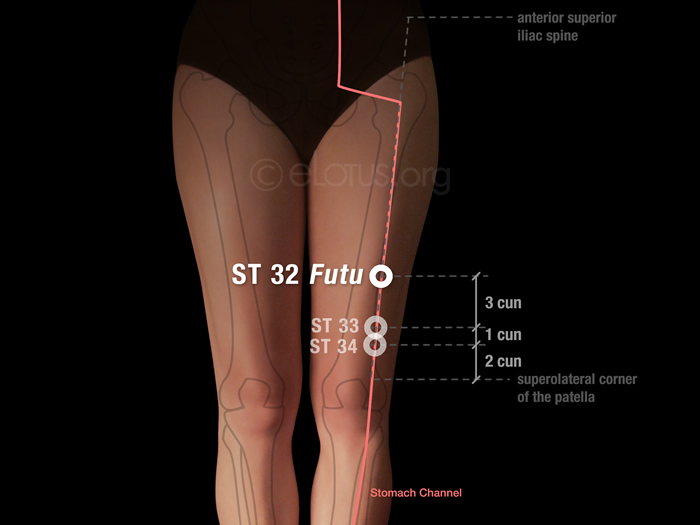
\includegraphics[width=\linewidth]{ST_32.jpg}\caption{Hình minh họa huyệt ST 32.}\end{figure}
\subsection*{Chỉ định}Đau vùng thắt lưng-chậu; liệt, hạn chế vận động và đau chi dưới; lạnh gối; cước khí.
\subsection*{Ứng dụng}Thông kinh, giảm đau; khu phong thấp, khu phong nhiệt, tán hàn.
\subsection*{Thủ thuật và lưu ý}Châm thẳng 0,7--1,2 thốn.

\subsection{ST 33 - Âm Thị (Yinshi)}
\subsection*{Thông tin cơ bản}\begin{description}\item[Hán tự và phiên âm:] 陰市; yīn shì.\item[Ý nghĩa tên:] Chợ Âm (dịch sát nghĩa; literal translation); tiếng Anh nguồn: Yin Market.\end{description}
\subsection*{Vị trí}Trên đường nối gai chậu trước trên với bờ ngoài xương bánh chè, cách góc trên-ngoài bánh chè 3 thốn về phía trên.
\begin{figure}[H]\centering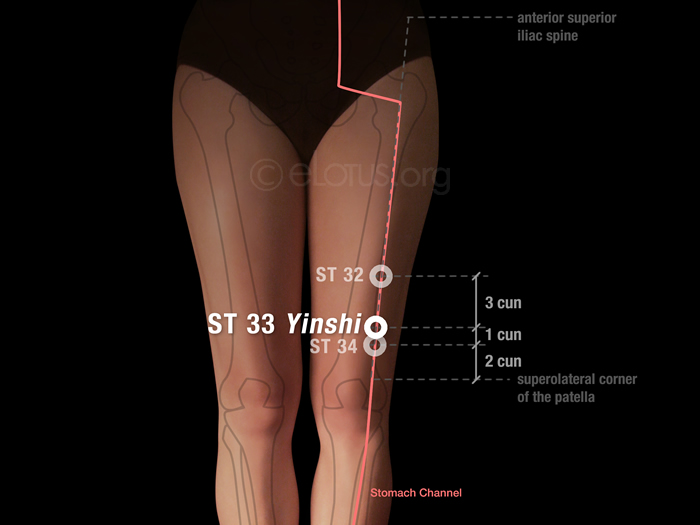
\includegraphics[width=\linewidth]{ST_33.jpg}\caption{Hình minh họa huyệt ST 33.}\end{figure}
\subsection*{Chỉ định}Tê, đau mỏi, hạn chế vận động chi dưới.
\subsection*{Ứng dụng}Thông kinh, giảm đau; khu phong thấp, tán hàn.
\subsection*{Thủ thuật và lưu ý}Châm thẳng 0,7--1 thốn.

\subsection{ST 34 - Lương Khâu (Liangqiu)}
\subsection*{Thông tin cơ bản}\begin{description}\item[Hán tự và phiên âm:] 梁丘; liáng qiū.\item[Ý nghĩa tên:] Gò xà (dịch sát nghĩa; literal translation); tiếng Anh nguồn: Beam Hill.\end{description}
\subsection*{Vị trí}Trên đường nối gai chậu trước trên với bờ ngoài xương bánh chè, cách góc trên-ngoài bánh chè 2 thốn về phía trên.
\begin{figure}[H]\centering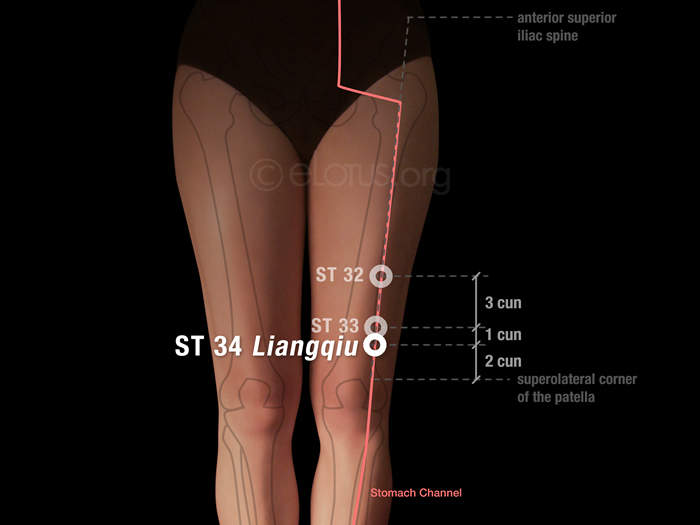
\includegraphics[width=\linewidth]{ST_34.jpg}\caption{Hình minh họa huyệt ST 34.}\end{figure}
\subsection*{Chỉ định}Đau dạ dày; viêm tuyến vú; đau, sưng, tê gối; hạn chế vận động chi dưới.
\subsection*{Ứng dụng}Điều hòa Vị, giảm đau; thông kinh; điều hòa tình trạng cấp.
\subsection*{Thủ thuật và lưu ý}Châm thẳng 0,7--1 thốn. Khích huyệt của kinh Vị.

\subsection{ST 35 - Độc Tỵ (Dubi)}
\subsection*{Thông tin cơ bản}\begin{description}\item[Hán tự và phiên âm:] 犢鼻; dú bí.\item[Ý nghĩa tên:] Mũi bắp chân (dịch sát nghĩa; literal translation); tiếng Anh nguồn: Calf Nose.\end{description}
\subsection*{Vị trí}Khi gối gấp, ở bờ dưới xương bánh chè, trong hõm phía ngoài dây chằng bánh chè.
\begin{figure}[H]\centering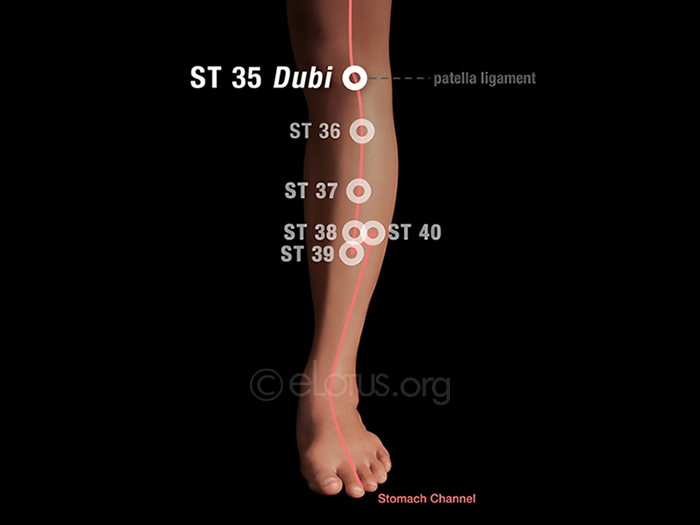
\includegraphics[width=\linewidth]{ST_35.jpg}\caption{Hình minh họa huyệt ST 35.}\end{figure}
\subsection*{Chỉ định}Đau, tê, hạn chế vận động gối; cước khí.
\subsection*{Ứng dụng}Khu phong thấp, giảm sưng; thông kinh, giảm đau.
\subsection*{Thủ thuật và lưu ý}Châm thẳng 0,7--1 thốn.

\subsection{ST 36 - Túc Tam Lý (Zusanli)}
\subsection*{Thông tin cơ bản}\begin{description}\item[Hán tự và phiên âm:] 足三里; zú sān lǐ.\item[Ý nghĩa tên:] Ba lý ở chân (dịch sát nghĩa; literal translation); tiếng Anh nguồn: Leg Three Li.\end{description}
\subsection*{Vị trí}Cách Độc Tỵ (ST 35) 3 thốn phía dưới, cách bờ trước xương chày một khoát ngón tay về phía ngoài.
\begin{figure}[H]\centering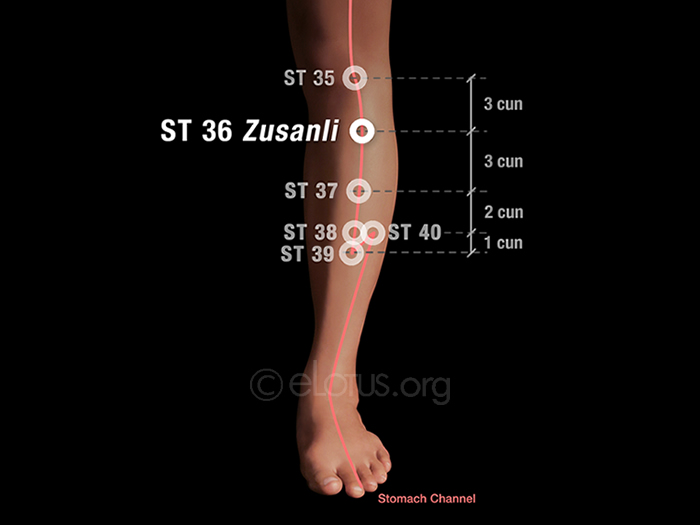
\includegraphics[width=\linewidth]{ST_36.jpg}\caption{Hình minh họa huyệt ST 36.}\end{figure}
\subsection*{Chỉ định}Khó tiêu, đau dạ dày, nôn, nấc, chướng bụng, sôi bụng, tiêu chảy, lỵ, táo bón, viêm ruột; viêm tuyến vú; đau gối và chân, cước khí, phù; ho, hen; gầy yếu do hư; đột quỵ, liệt nửa người; chóng mặt, mất ngủ, hưng cảm.
\subsection*{Ứng dụng}Điều hòa Tỳ Vị và ruột; điều khí, hóa thấp; bổ khí; thông kinh, giảm đau.
\subsection*{Thủ thuật và lưu ý}Châm thẳng 1--2 thốn. Ngũ hành thuộc Thổ; huyệt Du thuộc Thổ; Hợp huyệt, Hạ Hợp huyệt của Vị; huyệt Mẹ.

\subsection{ST 37 - Thượng Cự Hư (Shangjuxu)}
\subsection*{Thông tin cơ bản}\begin{description}\item[Hán tự và phiên âm:] 上巨虛; shàng jù xū.\item[Ý nghĩa tên:] Hốc lớn phía trên (dịch sát nghĩa; literal translation); tiếng Anh nguồn: Upper Great Hollow.\end{description}
\subsection*{Vị trí}Cách Độc Tỵ (ST 35) 6 thốn phía dưới, cách bờ trước xương chày một khoát ngón tay về phía ngoài.
\begin{figure}[H]\centering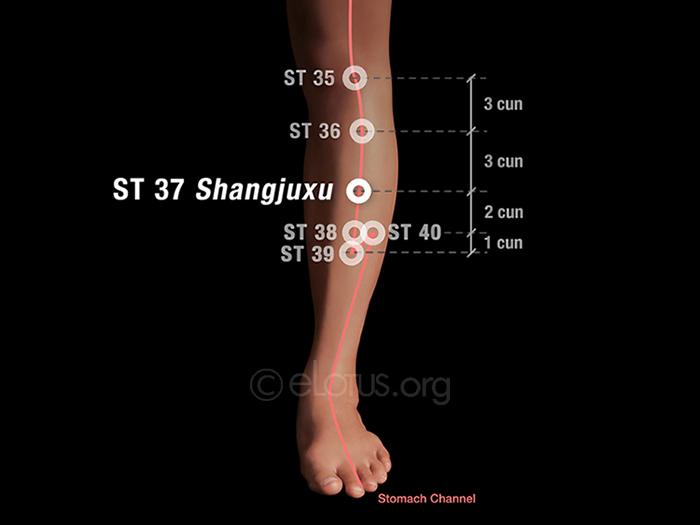
\includegraphics[width=\linewidth]{ST_37.jpg}\caption{Hình minh họa huyệt ST 37.}\end{figure}
\subsection*{Chỉ định}Đau, chướng bụng, sôi bụng; tiêu chảy, lỵ, táo bón, viêm ruột; liệt do đột quỵ; cước khí.
\subsection*{Ứng dụng}Điều hòa ruột, hóa trệ; thanh thấp nhiệt; điều hòa Tỳ, Vị và ruột; thông kinh, giảm đau.
\subsection*{Thủ thuật và lưu ý}Châm thẳng 1--1,5 thốn. Hạ Hợp huyệt của Đại Trường.

\subsection{ST 38 - Điều Khẩu (Tiaokou)}
\subsection*{Thông tin cơ bản}\begin{description}\item[Hán tự và phiên âm:] 條口; tiáo kǒu.\item[Ý nghĩa tên:] Miệng điều tiết (dịch sát nghĩa; literal translation); tiếng Anh nguồn: Ribbon Opening.\end{description}
\subsection*{Vị trí}Cách Độc Tỵ (ST 35) 8 thốn phía dưới, cách bờ trước xương chày một khoát ngón tay về phía ngoài.
\begin{figure}[H]\centering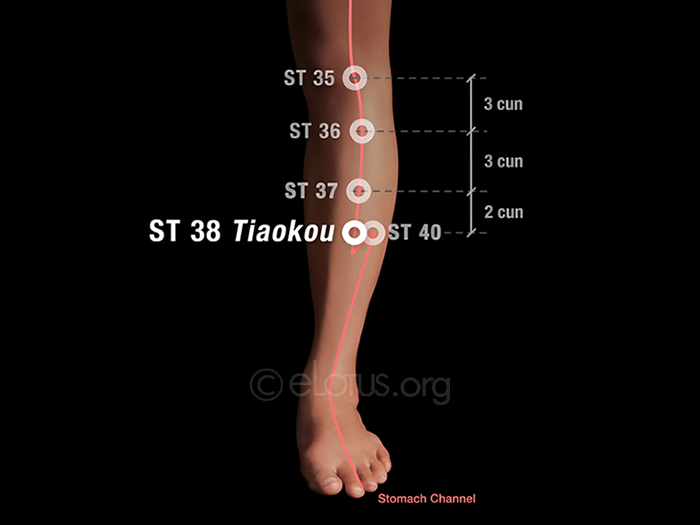
\includegraphics[width=\linewidth]{ST_38.jpg}\caption{Hình minh họa huyệt ST 38.}\end{figure}
\subsection*{Chỉ định}Tê, đau mỏi gối và chân; yếu, hạn chế vận động bàn chân; đau bụng; đau, hạn chế vận động vai.
\subsection*{Ứng dụng}Khu phong thấp, giảm đau; lợi vai.
\subsection*{Thủ thuật và lưu ý}Châm thẳng 1--1,5 thốn.

\subsection{ST 39 - Hạ Cự Hư (Xiajuxu)}
\subsection*{Thông tin cơ bản}\begin{description}\item[Hán tự và phiên âm:] 下巨虛; xià jù xū.\item[Ý nghĩa tên:] Hốc lớn phía dưới (dịch sát nghĩa; literal translation); tiếng Anh nguồn: Lower Great Hollow.\end{description}
\subsection*{Vị trí}Cách Độc Tỵ (ST 35) 9 thốn phía dưới, cách bờ trước xương chày một khoát ngón tay về phía ngoài.
\begin{figure}[H]\centering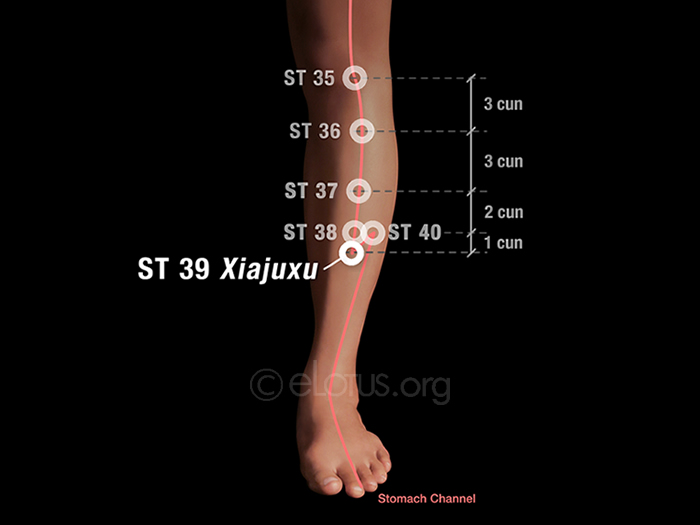
\includegraphics[width=\linewidth]{ST_39.jpg}\caption{Hình minh họa huyệt ST 39.}\end{figure}
\subsection*{Chỉ định}Đau bụng dưới; đau lưng lan đến tinh hoàn; tê, liệt chi dưới; viêm tuyến vú.
\subsection*{Ứng dụng}Điều khí Tiểu Trường, hóa trệ; điều hòa ruột, thanh thấp nhiệt; thông kinh, giảm đau.
\subsection*{Thủ thuật và lưu ý}Châm thẳng 1--1,5 thốn. Hạ Hợp huyệt của Tiểu Trường.

\subsection{ST 40 - Phong Long (Fenglong)}
\subsection*{Thông tin cơ bản}\begin{description}\item[Hán tự và phiên âm:] 豐隆; fēng lóng.\item[Ý nghĩa tên:] Gò phồng thịnh (dịch sát nghĩa; literal translation); tiếng Anh nguồn: Bountiful Bulge.\end{description}
\subsection*{Vị trí}Cách đỉnh mắt cá ngoài 8 thốn phía trên, cách bờ trước xương chày hai khoát ngón tay về phía ngoài (tức ngoài Điều Khẩu ST 38 một khoát ngón tay).
\begin{figure}[H]\centering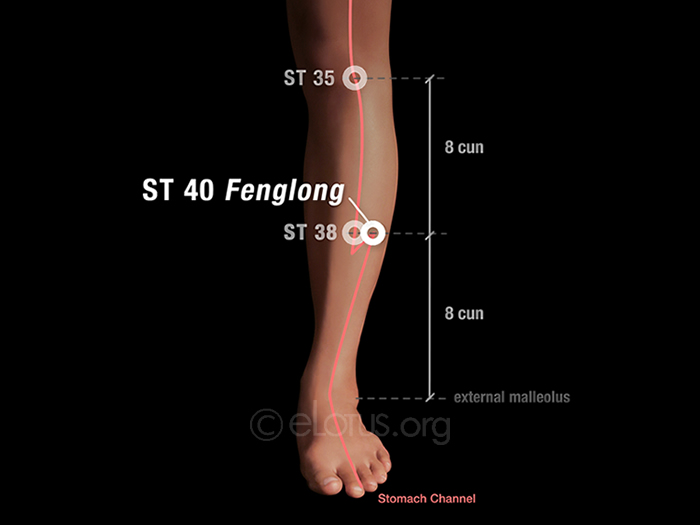
\includegraphics[width=\linewidth]{ST_40.jpg}\caption{Hình minh họa huyệt ST 40.}\end{figure}
\subsection*{Chỉ định}Đau đầu, chóng mặt, choáng váng, đau ngực; ho, hen, nhiều đờm, hưng cảm, động kinh; táo bón; teo cơ, hạn chế vận động, đau, sưng, liệt chi dưới.
\subsection*{Ứng dụng}Hóa đàm thấp, lợi ngực; thanh đàm ở Phế và Tâm, an thần; thông kinh, giảm đau.
\subsection*{Thủ thuật và lưu ý}Châm thẳng 1--1,5 thốn. Lạc huyệt của kinh Vị.

\subsection{ST 41 - Giải Khê (Jiexi)}
\subsection*{Thông tin cơ bản}\begin{description}\item[Hán tự và phiên âm:] 解谿; jiě xī.\item[Ý nghĩa tên:] Khe núi chia cắt (dịch sát nghĩa; literal translation); tiếng Anh nguồn: Ravine Divide.\end{description}
\subsection*{Vị trí}Ở mu chân, giữa nếp gấp ngang khớp cổ chân, trong hõm giữa gân cơ duỗi các ngón chân dài và gân cơ duỗi ngón cái dài, ngang đỉnh mắt cá ngoài.
\begin{figure}[H]\centering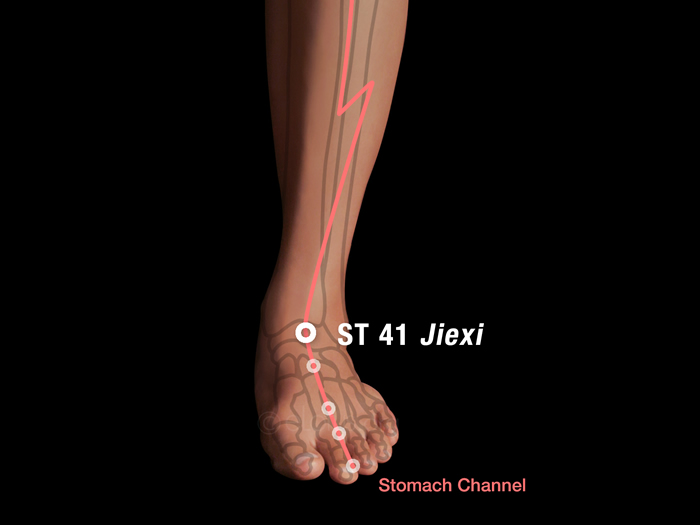
\includegraphics[width=\linewidth]{ST_41.jpg}\caption{Hình minh họa huyệt ST 41.}\end{figure}
\subsection*{Chỉ định}Chướng bụng, táo bón; động kinh, đau đầu, chóng mặt, choáng váng; đau cổ chân, teo cơ, hạn chế vận động, đau, liệt chi dưới.
\subsection*{Ứng dụng}Thanh nhiệt kinh Vị và phủ; an thần; thông kinh, giảm đau.
\subsection*{Thủ thuật và lưu ý}Châm thẳng 0,5--1 thốn. Ngũ hành thuộc Hỏa; huyệt Kinh thuộc Hỏa; huyệt Mẹ của kinh Vị.

\subsection{ST 42 - Xung Dương (Chongyang)}
\subsection*{Thông tin cơ bản}\begin{description}\item[Hán tự và phiên âm:] 沖陽; chōng yáng.\item[Ý nghĩa tên:] Dương xung (dịch sát nghĩa; literal translation); tiếng Anh nguồn: Surging Yang.\end{description}
\subsection*{Vị trí}Ở mu chân, cách Giải Khê (ST 41) 1,5 thốn về phía ngón chân, trong hõm giữa xương bàn chân 2-3 và xương chêm, nơi sờ thấy động mạch mu chân đập.
\begin{figure}[H]\centering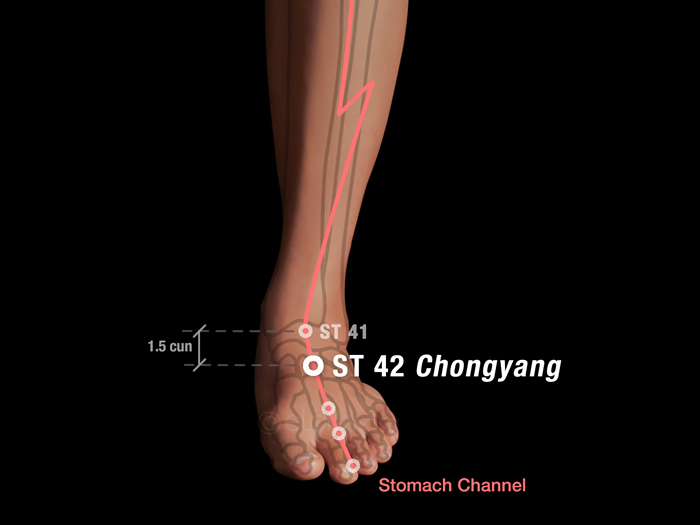
\includegraphics[width=\linewidth]{ST_42.jpg}\caption{Hình minh họa huyệt ST 42.}\end{figure}
\subsection*{Chỉ định}Đau răng hàm trên, liệt mặt; đỏ, sưng mu chân; teo cơ, hạn chế vận động bàn chân.
\subsection*{Ứng dụng}Điều hòa Vị, trấn kinh; thông kinh, giảm đau.
\subsection*{Thủ thuật và lưu ý}Châm thẳng 0,3--0,5 thốn; tránh chọc vào động mạch mu chân. Nguyên huyệt của kinh Vị; huyệt Xuất.

\subsection{ST 43 - Hãm Cốc (Xiangu)}
\subsection*{Thông tin cơ bản}\begin{description}\item[Hán tự và phiên âm:] 陷谷; xiàn gǔ.\item[Ý nghĩa tên:] Thung lũng lõm (dịch sát nghĩa; literal translation); tiếng Anh nguồn: Sunken Valley.\end{description}
\subsection*{Vị trí}Trong hõm phía xa chỗ nối xương bàn chân 2 và 3, cách Nội Đình (ST 44) 1 thốn về phía gần.
\begin{figure}[H]\centering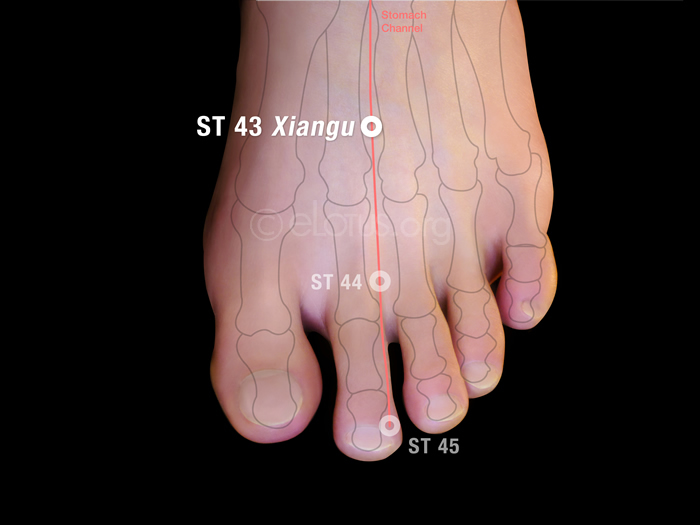
\includegraphics[width=\linewidth]{ST_43.jpg}\caption{Hình minh họa huyệt ST 43.}\end{figure}
\subsection*{Chỉ định}Phù mặt hoặc phù toàn thân; đau bụng, sôi bụng; sưng đau mu chân.
\subsection*{Ứng dụng}Điều hòa Tỳ, trừ thấp; điều hòa Vị và ruột.
\subsection*{Thủ thuật và lưu ý}Châm thẳng 0,5--0,8 thốn. Ngũ hành thuộc Mộc; huyệt Du thuộc Mộc.

\subsection{ST 44 - Nội Đình (Neiting)}
\subsection*{Thông tin cơ bản}\begin{description}\item[Hán tự và phiên âm:] 內庭; nèi tíng.\item[Ý nghĩa tên:] Sân trong (dịch sát nghĩa; literal translation); tiếng Anh nguồn: Inner Court.\end{description}
\subsection*{Vị trí}Gần bờ kẽ ngón 2-3, trong hõm phía xa và phía ngoài khớp bàn-ngón chân thứ hai.
\begin{figure}[H]\centering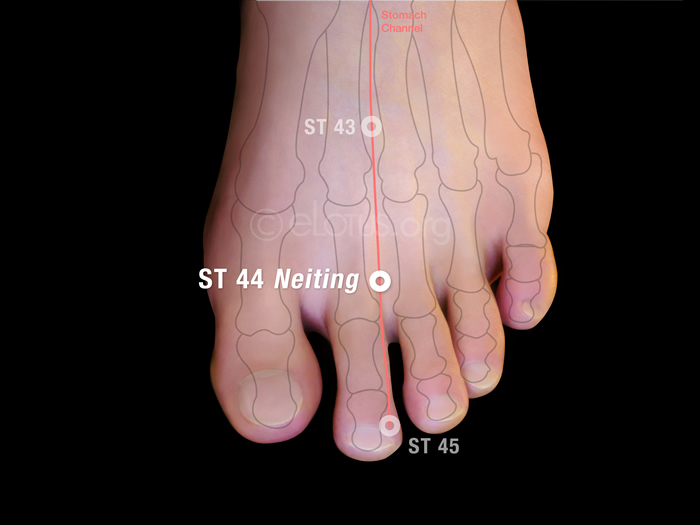
\includegraphics[width=\linewidth]{ST_44.jpg}\caption{Hình minh họa huyệt ST 44.}\end{figure}
\subsection*{Chỉ định}Đau răng, đau mặt, méo miệng, chảy máu cam, đau họng; đau dạ dày, trào ngược axit, chướng bụng, tiêu chảy, lỵ, táo bón; sưng đau mu chân; bệnh sốt.
\subsection*{Ứng dụng}Thanh nhiệt kinh Vị, giảm đau; điều hòa ruột, thanh thấp nhiệt; an thần.
\subsection*{Thủ thuật và lưu ý}Châm thẳng 0,5--0,8 thốn. Ngũ hành thuộc Thủy; huyệt Huỳnh thuộc Thủy; huyệt Con của kinh Vị.

\subsection{ST 45 - Lệ Đoài (Lidui)}
\subsection*{Thông tin cơ bản}\begin{description}\item[Hán tự và phiên âm:] 厲兌; lì duì.\item[Ý nghĩa tên:] Miệng nghiêm khắc (dịch sát nghĩa; literal translation); tiếng Anh nguồn: Severe Mouth.\end{description}
\subsection*{Vị trí}Ở phía ngoài ngón chân thứ hai, cách góc móng 0,1 thốn về phía sau.
\begin{figure}[H]\centering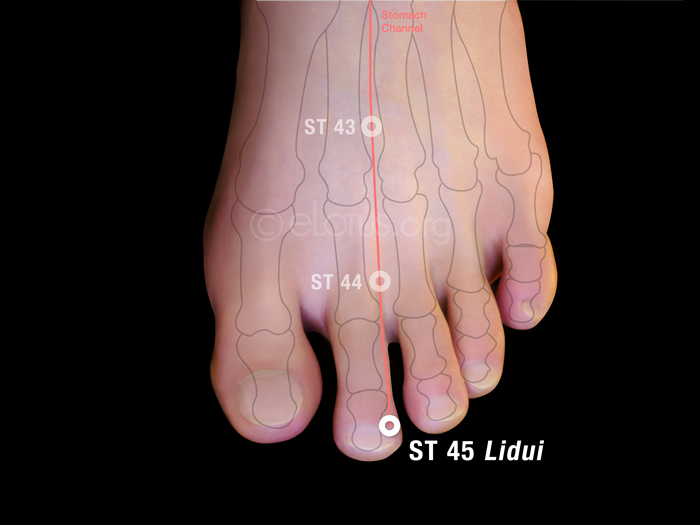
\includegraphics[width=\linewidth]{ST_45.jpg}\caption{Hình minh họa huyệt ST 45.}\end{figure}
\subsection*{Chỉ định}Sưng mặt, méo miệng, chảy máu cam, đau răng, đau họng, khàn tiếng; chướng bụng; lạnh chân và cẳng chân; bệnh sốt, ngủ mê do mộng, hưng cảm.
\subsection*{Ứng dụng}Thanh nhiệt, an thần; hồi tỉnh.
\subsection*{Thủ thuật và lưu ý}Châm xiên 0,1 thốn hoặc chích nặn máu. Ngũ hành thuộc Kim; huyệt Tỉnh thuộc Kim; huyệt Con của kinh Vị.
\clearpage
\section{Kinh Túc Thái Âm Tỳ}
\begin{description}
\item[Tên kinh/mạch:] Kinh Túc Thái Âm Tỳ (Tỳ) .
\item[Hán tự và phiên âm:] 足太陰脾經; zú tài yīn pí jīng.
\item[Thời gian hoạt động:] 9--11 giờ sáng.
\item[Ngũ hành:] Thổ.
\item[Kinh biểu lý:] Túc Dương Minh Vị.
\end{description}
\subsection*{Đường đi và phạm vi}Kinh Tỳ bắt nguồn từ Ẩn Bạch (SP 1) . Kinh chạy dọc theo mặt trong của bàn chân tại điểm nối của da đỏ và da trắng và đi lên phía trước mắt cá trong cho đến mặt trong của chân. Kinh đi theo mặt sau của xương chày, băng qua phía trước kinh Can. Đi qua mặt trước trong của đầu gối và đùi, kinh đi qua Trung Cực (CV 3) và Quan Nguyên (CV 4) rồi đi vào bụng. Sau đó đi qua Hạ Quản (CV 10) đến tạng Tỳ và kết nối với Vị. Từ đó kinh đi lên, đi qua cơ hoành tại Nhật Nguyệt (GB 24), Kỳ môn (LR 14) và Trung Phủ (LU 1) và chạy dọc theo thực quản. Khi nó đến gốc lưỡi, lan ra bề mặt dưới của nó. Nhánh từ Vị đi lên qua cơ hoành và đi vào Tâm, nơi nó kết nối với kinh Tâm.
\subsection*{Chỉ định của kinh/mạch}Đau thượng vị, nôn mửa, ợ hơi, phân lỏng, mệt mỏi, vàng da, chướng bụng; Cứng và đau ở gốc lưỡi; Cảm giác lạnh ở vùng giữa đầu gối và đùi;
\subsection*{Ứng dụng của kinh/mạch}Chủ vận hóa; Điều khiển sự thăng của khí; Chủ sinh huyết; Chủ cơ nhục và tứ chi; Khai khiếu ở miệng, biểu hiện ra môi; Chủ tân dịch; Tàng Ý (Yi); Gốc của khí hậu thiên, nguồn gốc ra đời và phát triển;
\subsection*{Phương pháp cân bằng}
\begin{enumerate}
\item Kinh Thủ Thái Âm Phế.
\item Kinh Thủ Thái Dương Tiểu Trường.
\item Kinh Túc Dương Minh Vị.
\item Kinh Thủ Thiếu Dương Tam Tiêu.
\item Kinh Thủ Thiếu Âm Tâm.
\end{enumerate}
\subsection*{Các huyệt đặc biệt}
\begin{itemize}
\item Tỉnh (Jing-Well): Ẩn Bạch (SP1).
\item Huỳnh (Ying-Spring): Đại Đô (SP2).
\item Du (Shu-Stream): Thái Bạch (SP3).
\item Kinh (Jing-River): Thương Khâu (SP5).
\item Hợp (He-Sea): Âm Lăng Tuyền (SP9).
\item Nguyên huyệt: Thái Bạch (SP3).
\item Lạc huyệt: Công Tôn (SP4).
\item Khích huyệt: Địa Cơ (SP8).
\item Mộ huyệt trước: Chương môn (LR13).
\item Du huyệt sau: Tỳ Du (BL20).
\item Huyệt Mẹ: Đại Đô (SP2).
\item Huyệt Con: Thương Khâu (SP5).
\item Huyệt Nhập: Ẩn Bạch (SP1).
\item Huyệt Xuất: Đại Bao (SP21).
\end{itemize}
\subsection{SP 1 - Ẩn Bạch (Yinbai)}
\subsection*{Thông tin cơ bản}\begin{description}\item[Hán tự và phiên âm:] 隱白; yǐn bái.\item[Ý nghĩa tên (theo tiếng Anh nguồn):] Trắng ẩn (dịch sát nghĩa; literal translation); tiếng Anh nguồn: Hidden White.\end{description}
\subsection*{Vị trí}Ở mặt trong của ngón chân cái, cách góc móng 0,1 thốn.
\begin{figure}[H]\centering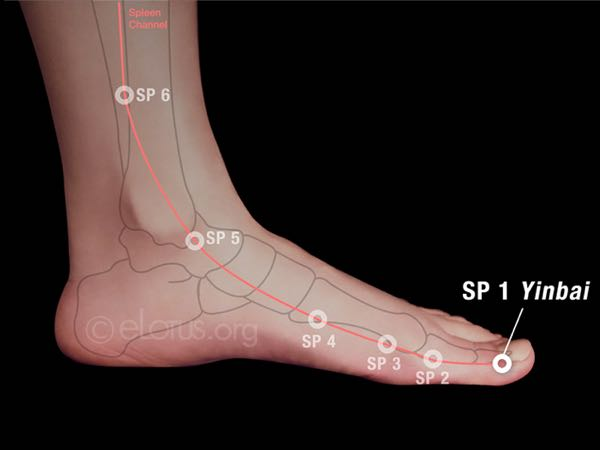
\includegraphics[width=\linewidth]{images/optimized/point_sp1.jpg}\caption{Hình minh họa huyệt SP 1.}\end{figure}
\subsection*{Chỉ định}Bụng chướng, phân có huyết; Rong kinh, chảy huyết tử thống; Rối loạn tâm thần, rối loạn giấc ngủ, co giật;
\subsection*{Ứng dụng}Điều hòa Tỳ và huyết ; Làm dịu Tâm và tinh thần và phục hồi ý thức;
\subsection*{Thủ thuật}Châm dưới da 0,1 thốn.
\subsection*{Phân loại và ghi chú}Điểm đặc biệt Ghi chú: Huyệt Tỉnh (Gỗ) - Tỳ Huyệt Nhập - SP 13 Quỷ huyệt - Fortress
\subsection{SP 2 - Đại Đô (Dadu)}
\subsection*{Thông tin cơ bản}\begin{description}\item[Hán tự và phiên âm:] 大都; dà dū.\item[Ý nghĩa tên (theo tiếng Anh nguồn):] Kinh đô lớn (dịch sát nghĩa; literal translation); tiếng Anh nguồn: Great Metropolis, Big Capital.\end{description}
\subsection*{Vị trí}Ở mặt trong ngón chân cái, xa và kém hơn khớp bàn ngón chân thứ nhất, ở chỗ lõm ở chỗ nối của da đỏ và da trắng.
\begin{figure}[H]\centering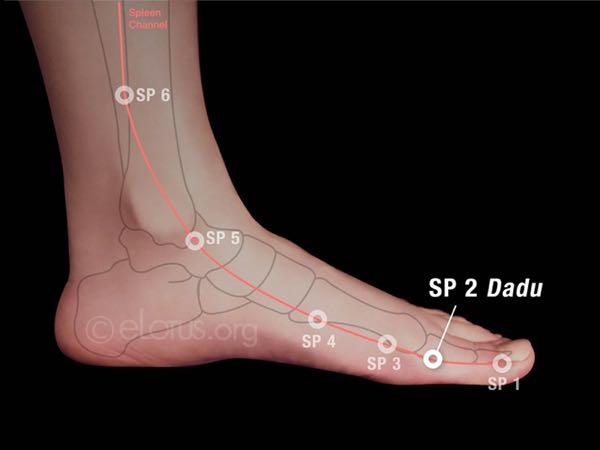
\includegraphics[width=\linewidth]{images/optimized/point_sp2.jpg}\caption{Hình minh họa huyệt SP 2.}\end{figure}
\subsection*{Chỉ định}Chướng bụng, đau Vị, táo bón ; Bệnh sốt kèm theo bệnh anhidrosis ;
\subsection*{Ứng dụng}Điều hòa Tỳ, điều hòa trung tiêu ; Giải quyết ẩm ướt, nhiệt ẩm, thanh nhiệt;
\subsection*{Thủ thuật}Châm thẳng 0,1-0,3 thốn.
\subsection*{Phân loại và ghi chú}Điểm đặc biệt Ghi chú: Điểm lò xo Ying (Lửa) - Tỳ
\subsection{SP 3 - Thái Bạch (Taibai)}
\subsection*{Thông tin cơ bản}\begin{description}\item[Hán tự và phiên âm:] 太白; taì bái.\item[Ý nghĩa tên (theo tiếng Anh nguồn):] Trắng tột bậc (dịch sát nghĩa; literal translation); tiếng Anh nguồn: Supreme White, Greater White.\end{description}
\subsection*{Vị trí}Ở mặt trong ngón chân cái, gần và dưới khớp bàn chân 1, ở chỗ lõm ở chỗ nối của da đỏ và da trắng.
\begin{figure}[H]\centering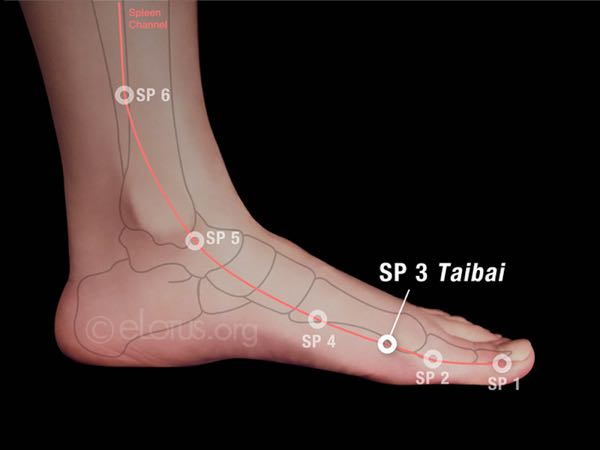
\includegraphics[width=\linewidth]{images/optimized/point_sp3.jpg}\caption{Hình minh họa huyệt SP 3.}\end{figure}
\subsection*{Chỉ định}Nôn mửa, borborygmus, đau Vị, chướng bụng, táo bón, kiết lỵ, tiêu chảy ; Cơ thể nặng nề, bệnh beriberi;
\subsection*{Ứng dụng}Bổ tỳ, giải trừ ẩm thấp; Điều hòa Tỳ và Vị; Điều hòa khí;
\subsection*{Thủ thuật}Châm thẳng 0,3-0,5 thốn. có thể cứu.
\subsection*{Phân loại và ghi chú}Điểm đặc biệt Ghi chú: Điểm suối Shu (Trái đất) - Tỳ Điểm nguồn Yuan - Tỳ
\subsection{SP 4 - Công Tôn (Gongsun)}
\subsection*{Thông tin cơ bản}\begin{description}\item[Hán tự và phiên âm:] 公孫; gōng sūn.\item[Ý nghĩa tên (theo tiếng Anh nguồn):] Hoàng Đế (dịch sát nghĩa; literal translation); tiếng Anh nguồn: Yellow Emperor, Ancestor and Descendant, Grandfather Grandson.\end{description}
\subsection*{Vị trí}Ở chỗ lõm xa và dưới gốc xương bàn chân 1, tại chỗ nối của da đỏ và da trắng.
\begin{figure}[H]\centering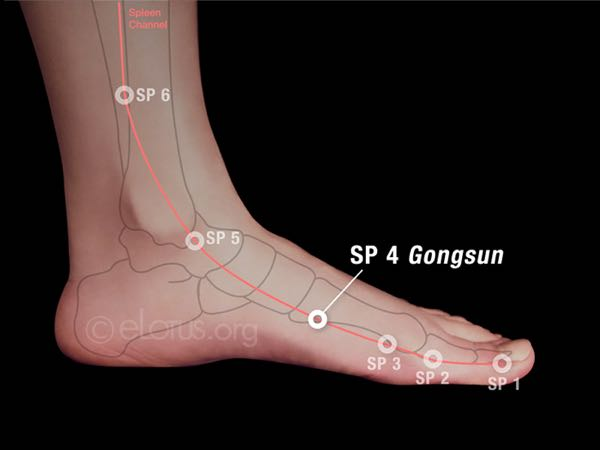
\includegraphics[width=\linewidth]{images/optimized/point_sp4.jpg}\caption{Hình minh họa huyệt SP 4.}\end{figure}
\subsection*{Chỉ định}Nôn mửa, đau Vị, đau bụng và chướng bụng, tiêu chảy, kiết lỵ, borborygmus ;
\subsection*{Ứng dụng}Tăng cường Tỳ và điều hòa trung tiêu ; Điều hòa khí và giải quyết ẩm ướt; Có lợi cho Tâm và ngực, an thần; Điều chỉnh kinh chong (đường cao tốc);
\subsection*{Thủ thuật}Châm thẳng 0,5-0,8 thốn.
\subsection*{Phân loại và ghi chú}Điểm đặc biệt Ghi chú: Điểm kết nối Luo - Điểm chính Tỳ - Kinh Chong (Đường cao tốc) Điểm ghép - Kinh Yinwei (Liên kết)
\subsection{SP 5 - Thương Khâu (Shangqiu)}
\subsection*{Thông tin cơ bản}\begin{description}\item[Hán tự và phiên âm:] 商丘; shāng qiū.\item[Ý nghĩa tên (theo tiếng Anh nguồn):] Gò Thương (dịch sát nghĩa; literal translation); tiếng Anh nguồn: Shang Hill, Metal Mound, Shang Mound.\end{description}
\subsection*{Vị trí}Trong chỗ lõm ở xa và dưới mắt cá trong, nằm giữa lồi xương thuyền và đầu mắt cá trong.
\begin{figure}[H]\centering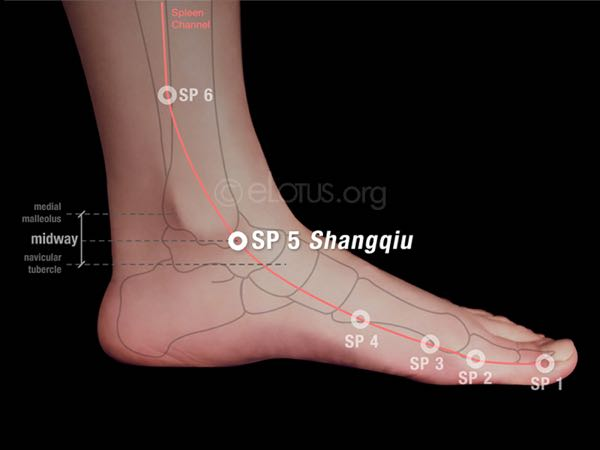
\includegraphics[width=\linewidth]{images/optimized/point_sp5.jpg}\caption{Hình minh họa huyệt SP 5.}\end{figure}
\subsection*{Chỉ định}Chướng bụng, táo bón, tiêu chảy, chán ăn ; Đau và cứng lưỡi; Đau ở bàn chân và mắt cá chân;
\subsection*{Ứng dụng}Tăng cường Tỳ và giải quyết ẩm ướt ; Lợi ích gân cốt ; An thần;
\subsection*{Thủ thuật}Châm thẳng 0,2-0,3 thốn.
\subsection*{Phân loại và ghi chú}Điểm đặc biệt Ghi chú: Huyệt Kinh (Kim loại) - Tỳ
\subsection{SP 6 - Tam Âm Giao (Sanyinjiao)}
\subsection*{Thông tin cơ bản}\begin{description}\item[Hán tự và phiên âm:] 三陰交; sān yīn jiāo.\item[Ý nghĩa tên (theo tiếng Anh nguồn):] Giao hội của ba kinh Âm (dịch sát nghĩa; literal translation); tiếng Anh nguồn: Three Yin Intersection, Three Yin Meeting.\end{description}
\subsection*{Vị trí}3 thốn ngay phía trên đầu mắt cá trong, phía sau bờ trong xương chày.
\begin{figure}[H]\centering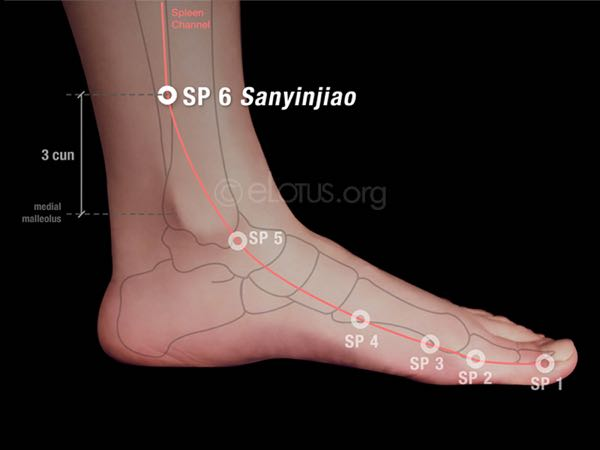
\includegraphics[width=\linewidth]{images/optimized/point_sp6.jpg}\caption{Hình minh họa huyệt SP 6.}\end{figure}
\subsection*{Chỉ định}Đau bụng, chán ăn, chướng bụng, tiêu chảy ; Kinh nguyệt không đều, chảy huyết tử thống, bệnh bạch cầu, sa tử thống, đau bụng kinh; Vô sinh, chậm chuyển dạ, xuất tinh về đêm, liệt dương, đau cơ quan sinh dục ngoài; Đái dầm, tiểu khó, phù nề, thoát vị; Teo cơ, suy giảm vận động, tê liệt và đau chi dưới; Đau đầu, chóng mặt và mất ngủ;
\subsection*{Ứng dụng}Bổ tỳ và Vị, giải quyết ẩm ướt ; Điều hòa Can và làm dịu dòng khí; Tăng cường Thận ; Điều hòa huyết, điều hòa kinh nguyệt và kích thích chuyển dạ; Điều hòa khí hư, điều hòa tiểu tiện và có lợi cho cơ quan sinh dục; An thần; Kích hoạt kinh và giảm đau;
\subsection*{Thủ thuật}Châm thẳng 0,5-1,0 thốn.
\subsection*{Phân loại và ghi chú}Phân loại và ghi chú: Nhóm Luo Point - 3 Chân Âm
\subsection{SP 7 - Lậu Cốc (Lougu)}
\subsection*{Thông tin cơ bản}\begin{description}\item[Hán tự và phiên âm:] 漏谷; loù gǔ.\item[Ý nghĩa tên (theo tiếng Anh nguồn):] Thung lũng rỉ nước (dịch sát nghĩa; literal translation); tiếng Anh nguồn: Leaking Valley, Dripping Valley, Seeping Valley.\end{description}
\subsection*{Vị trí}6 thốn phía trên đầu mắt cá trong, trên đường nối đầu mắt cá trong với Âm Lăng Tuyền (SP 9), phía sau bờ trong xương chày.
\begin{figure}[H]\centering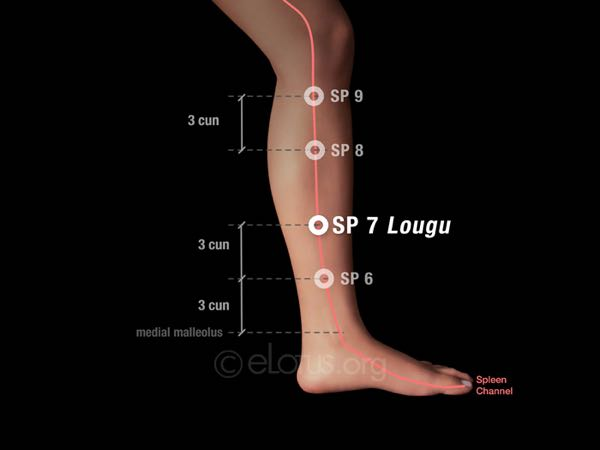
\includegraphics[width=\linewidth]{images/optimized/point_sp7.jpg}\caption{Hình minh họa huyệt SP 7.}\end{figure}
\subsection*{Chỉ định}Chướng bụng, borborygmus ; Lạnh, tê và tê liệt đầu gối và chân;
\subsection*{Ứng dụng}Tăng cường Tỳ và giải quyết ẩm ướt ; Thúc đẩy đi tiểu và phân tán sưng tấy;
\subsection*{Thủ thuật}Châm thẳng 0,5-1,0 thốn.
\subsection{SP 8 - Địa Cơ (Diji)}
\subsection*{Thông tin cơ bản}\begin{description}\item[Hán tự và phiên âm:] 地機; dì jī.\item[Ý nghĩa tên (theo tiếng Anh nguồn):] Trục của Đất (dịch sát nghĩa; literal translation); tiếng Anh nguồn: Earth's Crux, Earth Pivot.\end{description}
\subsection*{Vị trí}3 thốn phía dưới Âm Lăng Tuyền (SP 9), trên đường nối Âm Lăng Tuyền (SP 9) và mắt cá trong, ở chỗ lõm phía sau bờ trong xương chày.
\begin{figure}[H]\centering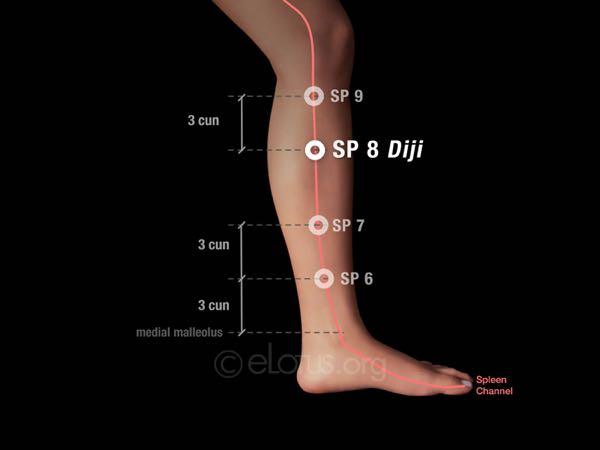
\includegraphics[width=\linewidth]{images/optimized/point_sp8.jpg}\caption{Hình minh họa huyệt SP 8.}\end{figure}
\subsection*{Chỉ định}Đau bụng và chướng bụng, tiêu chảy, phù nề, khó tiểu ; Khí hư về đêm, kinh nguyệt không đều, đau bụng kinh;
\subsection*{Ứng dụng}Điều hòa Tỳ và giải quyết ẩm ướt ; Điều hòa kinh nguyệt và bổ huyết; Điều kiện cấp tính vừa phải;
\subsection*{Thủ thuật}Châm thẳng 0,5-1,0 thốn.
\subsection*{Phân loại và ghi chú}Điểm đặc biệt Ghi chú: Khích huyệt - Tỳ
\subsection{SP 9 - Âm Lăng Tuyền (Yinlingquan)}
\subsection*{Thông tin cơ bản}\begin{description}\item[Hán tự và phiên âm:] 陰陵泉; yīn líng qúan.\item[Ý nghĩa tên (theo tiếng Anh nguồn):] Suối gò Âm (dịch sát nghĩa; literal translation); tiếng Anh nguồn: Yin Mound Spring.\end{description}
\subsection*{Vị trí}Trong chỗ lõm phía sau và dưới lồi cầu trong của xương chày, ở góc được tạo bởi lồi cầu trong và bờ sau của xương chày.
\begin{figure}[H]\centering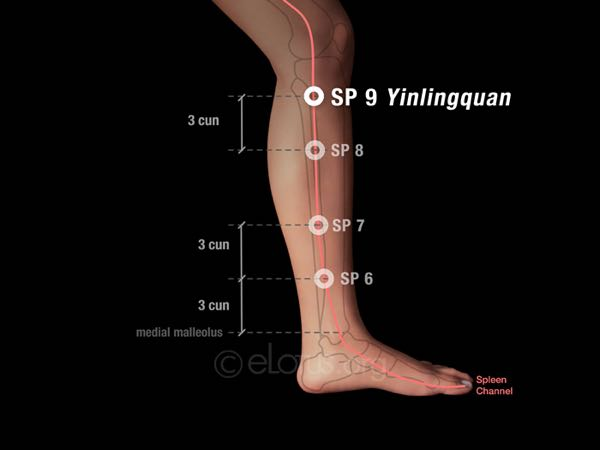
\includegraphics[width=\linewidth]{images/optimized/point_sp9.jpg}\caption{Hình minh họa huyệt SP 9.}\end{figure}
\subsection*{Chỉ định}Đau bụng và chướng bụng, tiêu chảy, kiết lỵ ; Phù, vàng da, khó tiểu, đái dầm, tiểu không tự chủ; Đau cơ quan sinh dục ngoài, đau bụng kinh; Đau đầu gối;
\subsection*{Ứng dụng}Điều hòa Tỳ và giải quyết ẩm ướt ; Mở và di chuyển các đường dẫn nước; Lợi ích hạ giao ;
\subsection*{Thủ thuật}Châm thẳng 0,5-1,0 thốn.
\subsection*{Phân loại và ghi chú}Điểm đặc biệt nhận xét: He Huyệt Hải (Nước) - Tỳ
\subsection{SP 10 - Huyết Hải (Xuehai)}
\subsection*{Thông tin cơ bản}\begin{description}\item[Hán tự và phiên âm:] 血海; xuè hǎi.\item[Ý nghĩa tên (theo tiếng Anh nguồn):] Biển máu (dịch sát nghĩa; literal translation); tiếng Anh nguồn: Sea of Blood.\end{description}
\subsection*{Vị trí}Khi gập đầu gối, điểm nằm cách bờ trong phía trên của xương bánh chè 2 thốn, trên chỗ lồi của phần trong của cơ tứ đầu đùi. Hoặc khi đầu gối của bệnh nhân gập lại, hãy đặt gót bàn tay phải của bạn lên xương bánh chè bên trái của bệnh nhân, ngón cái và các ngón khác duỗi thẳng hoàn toàn và ngón cái tạo một góc 45° với ngón trỏ. Vấn đề là nơi đầu ngón tay cái của bạn nằm.
\begin{figure}[H]\centering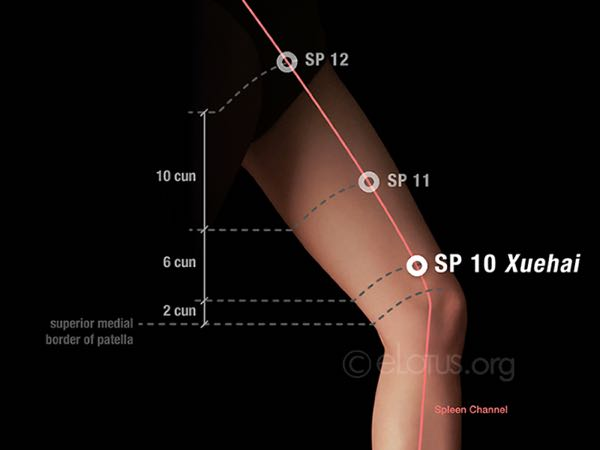
\includegraphics[width=\linewidth]{images/optimized/point_sp10.jpg}\caption{Hình minh họa huyệt SP 10.}\end{figure}
\subsection*{Chỉ định}Kinh nguyệt không đều, đau bụng kinh, chảy huyết tử thống, vô kinh ; Mề đay, chàm, ban đỏ; Đau ở mặt giữa của đùi;
\subsection*{Ứng dụng}Bổ huyết, mát huyết, tiêu huyết ứ, điều hòa kinh nguyệt; Có lợi cho da;
\subsection*{Thủ thuật}Châm thẳng 0,5-1,2 thốn.
\subsection{SP 11 - Cơ Môn (Jimen)}
\subsection*{Thông tin cơ bản}\begin{description}\item[Hán tự và phiên âm:] 箕門; jī mén.\item[Ý nghĩa tên (theo tiếng Anh nguồn):] Cửa sàng (dịch sát nghĩa; literal translation); tiếng Anh nguồn: Winnower Gate, Basket's Door.\end{description}
\subsection*{Vị trí}6 thốn gần Huyết Hải h Tu (SP 10) , trên đường rút từ Huyết Hải h Tu (SP 10) đến Xung Môn (SP 12) .
\begin{figure}[H]\centering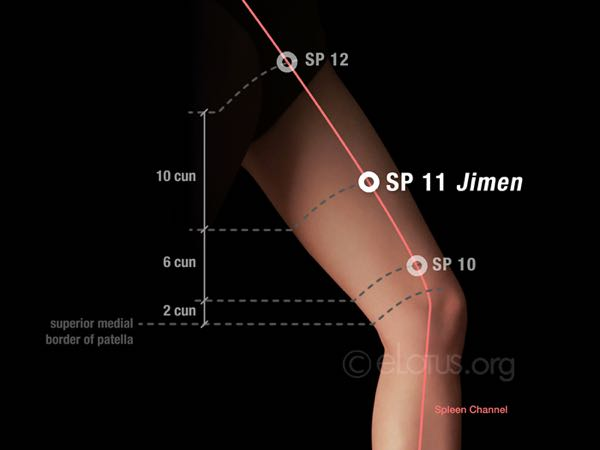
\includegraphics[width=\linewidth]{images/optimized/point_sp11.jpg}\caption{Hình minh họa huyệt SP 11.}\end{figure}
\subsection*{Chỉ định}Tiểu khó, đái dầm, đau và sưng ở vùng bẹn ; Teo cơ, suy giảm vận động, đau và tê liệt chi dưới;
\subsection*{Ứng dụng}Điều hòa tiểu tiện ; Thoát ẩm và giải nhiệt;
\subsection*{Thủ thuật}Châm thẳng 0,5-1,0 thốn. Không nên đưa sâu vào vì có thể làm thủng động mạch đùi.
\subsection{SP 12 - Xung Môn (Chongmen)}
\subsection*{Thông tin cơ bản}\begin{description}\item[Hán tự và phiên âm:] 沖門; chōng mén.\item[Ý nghĩa tên (theo tiếng Anh nguồn):] Cửa xung (dịch sát nghĩa; literal translation); tiếng Anh nguồn: Surging Gate, Rushing Gate, Rushing Door.\end{description}
\subsection*{Vị trí}Phía trên đầu bên của rãnh bẹn, bên ngoài động mạch đùi, ngang mức bờ trên của khớp mu, cách Qugu 3,5 thốn (CV 2).
\begin{figure}[H]\centering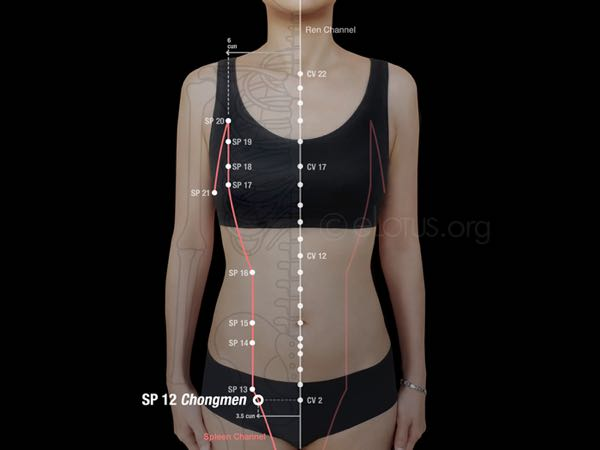
\includegraphics[width=\linewidth]{images/optimized/point_sp12.jpg}\caption{Hình minh họa huyệt SP 12.}\end{figure}
\subsection*{Chỉ định}Đau bụng, thoát vị ; Khó tiểu;
\subsection*{Ứng dụng}Tiếp thêm sinh lực, điều hòa khí, thông kinh; Thoát ẩm, thanh nhiệt, điều hòa tiểu tiện;
\subsection*{Thủ thuật}Châm thẳng 0,5-1,0 thốn. Không nên đưa sâu vào vì nó có thể làm thủng động mạch đùi theo hướng trong hoặc dây thần kinh đùi theo hướng bên.
\subsection{SP 13 - Phủ Xá (Fushe)}
\subsection*{Thông tin cơ bản}\begin{description}\item[Hán tự và phiên âm:] 府舍; fǔ shè.\item[Ý nghĩa tên (theo tiếng Anh nguồn):] Nhà của tạng phủ (dịch sát nghĩa; literal translation); tiếng Anh nguồn: Bowel Abode, Abode of the Fu, Dwelling.\end{description}
\subsection*{Vị trí}4,3 thốn phía dưới trung tâm rốn, 4 thốn phía ngoài đường giữa trước. Hoặc 0,7 thốn trên và 0,5 thốn bên Xung Môn (SP 12) .
\begin{figure}[H]\centering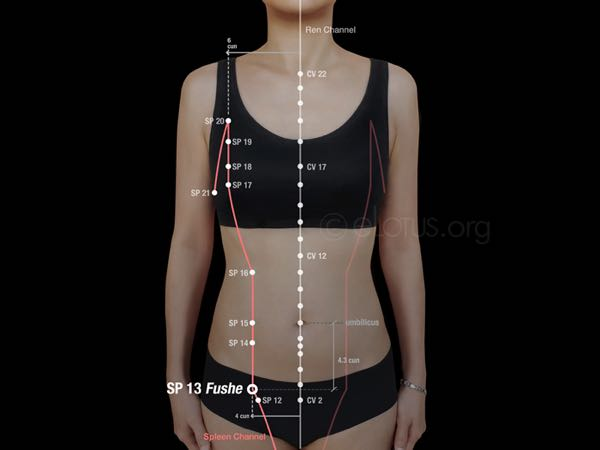
\includegraphics[width=\linewidth]{images/optimized/point_sp13.jpg}\caption{Hình minh họa huyệt SP 13.}\end{figure}
\subsection*{Chỉ định}Đau bụng dưới, thoát vị ;
\subsection*{Ứng dụng}Điều hòa khí và giảm đau;
\subsection*{Thủ thuật}Châm thẳng 0,5-1,0 thốn.
\subsection{SP 14 - Phúc Kết (Fujie)}
\subsection*{Thông tin cơ bản}\begin{description}\item[Hán tự và phiên âm:] 腹結; fù jié.\item[Ý nghĩa tên (theo tiếng Anh nguồn):] Nút thắt bụng (dịch sát nghĩa; literal translation); tiếng Anh nguồn: Abdominal Bind, Abdomen Knot.\end{description}
\subsection*{Vị trí}1,3 thốn phía dưới trung tâm rốn, 4 thốn về phía ngoài so với đường giữa trước, trên bờ ngoài của cơ thẳng bụng. Hoặc thấp hơn Daheng 1,3 thốn (SP 15) .
\begin{figure}[H]\centering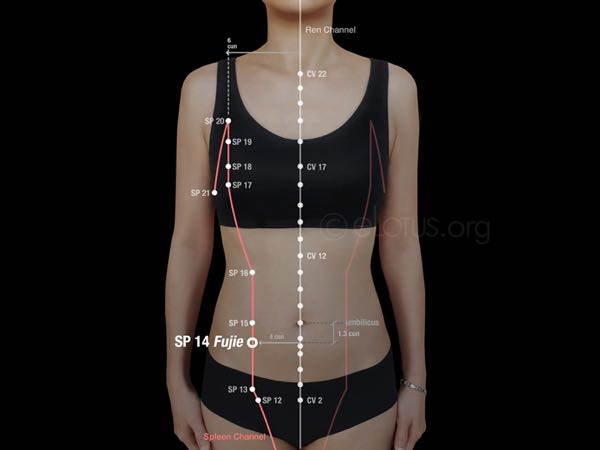
\includegraphics[width=\linewidth]{images/optimized/point_sp14.jpg}\caption{Hình minh họa huyệt SP 14.}\end{figure}
\subsection*{Chỉ định}Đau quanh vùng rốn ; Chướng bụng, tiêu chảy, táo bón, thoát vị;
\subsection*{Ứng dụng}Ấm áp và mang lại lợi ích cho hạ đẳng ; Điều hòa khí và hạ khí nổi loạn;
\subsection*{Thủ thuật}Châm thẳng 0,5-1,0 thốn.
\subsection{SP 15 - Đại Hoành (Daheng)}
\subsection*{Thông tin cơ bản}\begin{description}\item[Hán tự và phiên âm:] 大横; dà héng.\item[Ý nghĩa tên (theo tiếng Anh nguồn):] Ngang lớn (dịch sát nghĩa; literal translation); tiếng Anh nguồn: Great Horizontal, Big Horizontal Stroke.\end{description}
\subsection*{Vị trí}cách trung tâm rốn 4 thốn, ở chỗ lõm ở bờ ngoài của cơ thẳng bụng.
\begin{figure}[H]\centering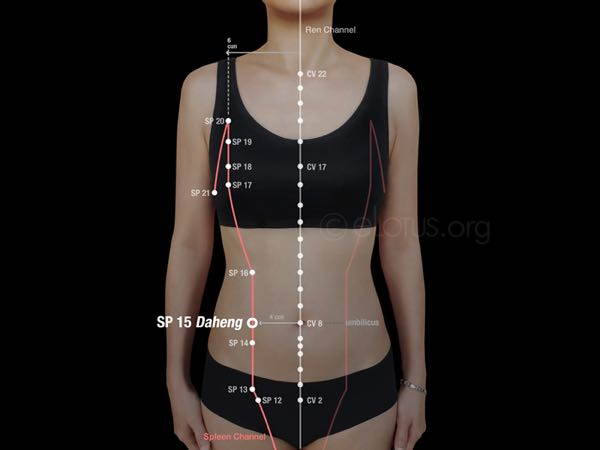
\includegraphics[width=\linewidth]{images/optimized/point_sp15.jpg}\caption{Hình minh họa huyệt SP 15.}\end{figure}
\subsection*{Chỉ định}Đau bụng và chướng bụng, tiêu chảy, lỵ, táo bón ;
\subsection*{Ứng dụng}Di chuyển khí và điều hòa đường ruột;
\subsection*{Thủ thuật}Châm thẳng 0,7-1,2 thốn.
\subsection{SP 16 - Phúc Ai (Fuai)}
\subsection*{Thông tin cơ bản}\begin{description}\item[Hán tự và phiên âm:] 腹哀; fù ā.\item[Ý nghĩa tên (theo tiếng Anh nguồn):] Nỗi buồn ở bụng (dịch sát nghĩa; literal translation); tiếng Anh nguồn: Abdominal Lament, Abdomen Sorrow.\end{description}
\subsection*{Vị trí}3 thốn phía trên trung tâm rốn, 4 thốn phía ngoài đường giữa trước ở bờ ngoài của cơ thẳng bụng, ngang với Kiến Lý (CV 11).
\begin{figure}[H]\centering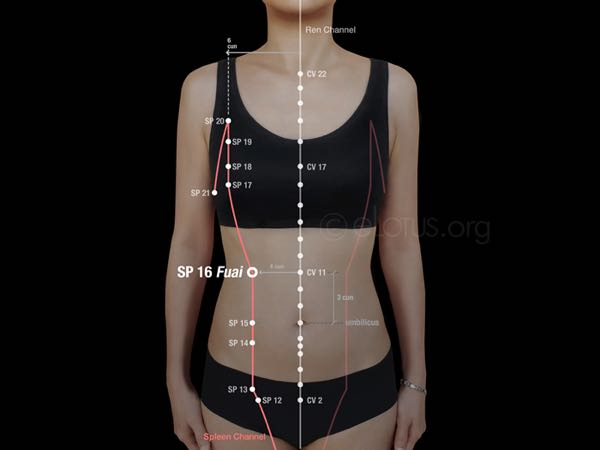
\includegraphics[width=\linewidth]{images/optimized/point_sp16.jpg}\caption{Hình minh họa huyệt SP 16.}\end{figure}
\subsection*{Chỉ định}Đau bụng, khó tiêu, táo bón, lỵ ;
\subsection*{Ứng dụng}Điều hòa đường ruột ;
\subsection*{Thủ thuật}Châm thẳng 0,5-1,0 thốn.
\subsection{SP 17 - Thực Đậu (Shidou)}
\subsection*{Thông tin cơ bản}\begin{description}\item[Hán tự và phiên âm:] 食竇; shí dòu.\item[Ý nghĩa tên (theo tiếng Anh nguồn):] Hốc thức ăn (dịch sát nghĩa; literal translation); tiếng Anh nguồn: Food Hole, Food Cavity.\end{description}
\subsection*{Vị trí}Ở khoang liên sườn 5, cách đường giữa trước 6 thốn.
\begin{figure}[H]\centering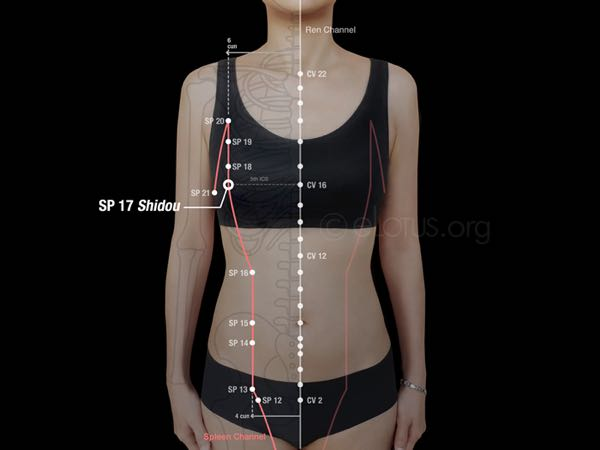
\includegraphics[width=\linewidth]{images/optimized/point_sp17.jpg}\caption{Hình minh họa huyệt SP 17.}\end{figure}
\subsection*{Chỉ định}Cảm giác đầy bụng, đau ở ngực và vùng hạ sườn ;
\subsection*{Ứng dụng}Làm tiêu tan sự tích tụ thức ăn và chất lỏng, thúc đẩy quá trình tiêu hóa;
\subsection*{Thủ thuật}Châm xiên 0,3-0,5 thốn. Không nên đặt vuông góc vì nó có thể gây tràn khí màng Phế.
\subsection{SP 18 - Thiên Khê (Tianxi)}
\subsection*{Thông tin cơ bản}\begin{description}\item[Hán tự và phiên âm:] 天谿; tiān xī.\item[Ý nghĩa tên (theo tiếng Anh nguồn):] Khe trời (dịch sát nghĩa; literal translation); tiếng Anh nguồn: Celestial Ravine, Heavenly Stream.\end{description}
\subsection*{Vị trí}Ở khoang liên sườn 4, cách đường giữa trước 6 thốn.
\begin{figure}[H]\centering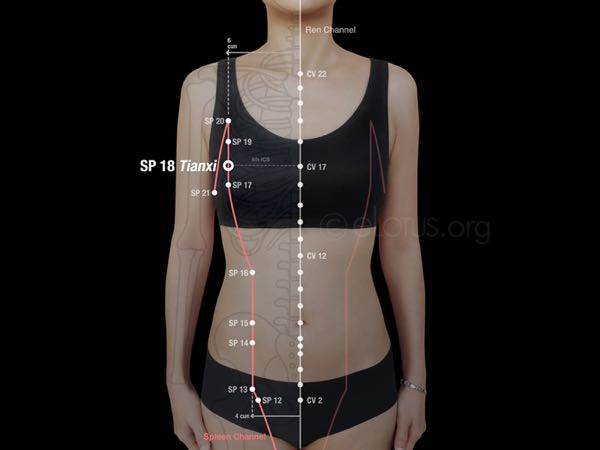
\includegraphics[width=\linewidth]{images/optimized/point_sp18.jpg}\caption{Hình minh họa huyệt SP 18.}\end{figure}
\subsection*{Chỉ định}Đầy và đau ở ngực và hạ sườn, ho, nấc ; Viêm vú, tiết sữa không đủ;
\subsection*{Ứng dụng}Điều hòa và hạ khí; Có lợi cho ngực và thúc đẩy tiết sữa;
\subsection*{Thủ thuật}Châm xiên 0,3-0,5 thốn. Không nên đặt vuông góc vì nó có thể gây tràn khí màng Phế.
\subsection{SP 19 - Hung Hương (Xiongxiang)}
\subsection*{Thông tin cơ bản}\begin{description}\item[Hán tự và phiên âm:] 胸鄉; xiōng xiāng.\item[Ý nghĩa tên (theo tiếng Anh nguồn):] Làng ngực (dịch sát nghĩa; literal translation); tiếng Anh nguồn: Chest Village, Chest Home.\end{description}
\subsection*{Vị trí}Ở khoang liên sườn 3, cách đường giữa trước 6 thốn.
\begin{figure}[H]\centering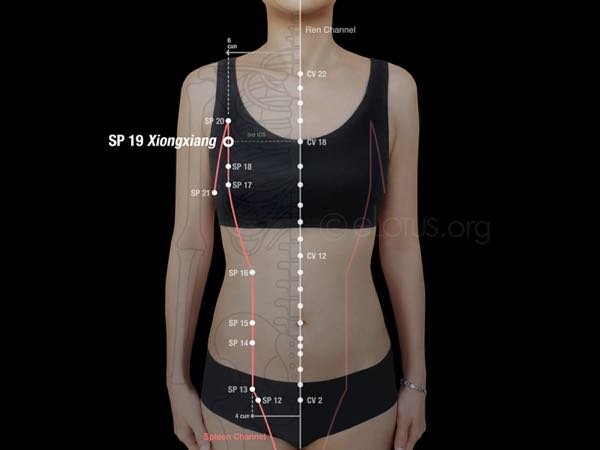
\includegraphics[width=\linewidth]{images/optimized/point_sp19.jpg}\caption{Hình minh họa huyệt SP 19.}\end{figure}
\subsection*{Chỉ định}Cảm giác đầy bụng, đau ở ngực và vùng hạ sườn ;
\subsection*{Ứng dụng}Điều hòa và hạ khí cũng như giải phóng lồng ngực ;
\subsection*{Thủ thuật}Châm xiên 0,3-0,5 thốn. Không nên đặt vuông góc vì nó có thể gây tràn khí màng Phế.
\subsection{SP 20 - Chu Vinh (Zhourong)}
\subsection*{Thông tin cơ bản}\begin{description}\item[Hán tự và phiên âm:] 周榮; zhōu róng.\item[Ý nghĩa tên (theo tiếng Anh nguồn):] Vinh quang bao quanh (dịch sát nghĩa; literal translation); tiếng Anh nguồn: All Round Flourishing, Encircling Glory.\end{description}
\subsection*{Vị trí}Ở khoang liên sườn thứ 2, cách đường giữa trước 6 thốn.
\begin{figure}[H]\centering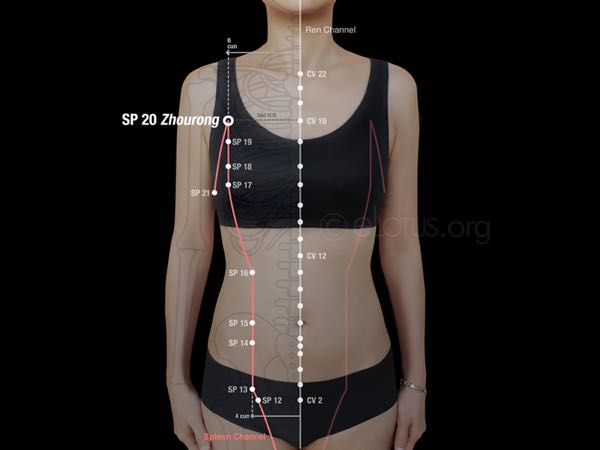
\includegraphics[width=\linewidth]{images/optimized/point_sp20.jpg}\caption{Hình minh họa huyệt SP 20.}\end{figure}
\subsection*{Chỉ định}Đầy đặn ở ngực và vùng hạ sườn ; Ho, nấc;
\subsection*{Ứng dụng}Điều hòa và hạ khí cũng như giải phóng lồng ngực ;
\subsection*{Thủ thuật}Châm xiên 0,3-0,5 thốn. Không nên đặt vuông góc vì nó có thể gây tràn khí màng Phế.
\subsection{SP 21 - Đại Bao (Dabao)}
\subsection*{Thông tin cơ bản}\begin{description}\item[Hán tự và phiên âm:] 大包; dà bāo.\item[Ý nghĩa tên (theo tiếng Anh nguồn):] Sự bao bọc lớn (dịch sát nghĩa; literal translation); tiếng Anh nguồn: Great Embracement, Great Wrapping, Big Wrapping.\end{description}
\subsection*{Vị trí}Ở phía bên của ngực, trên đường nách giữa, ở khoang liên sườn thứ 6.
\begin{figure}[H]\centering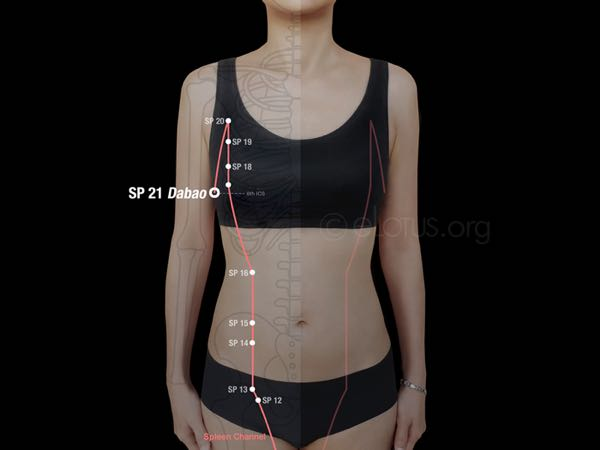
\includegraphics[width=\linewidth]{images/optimized/point_sp21.jpg}\caption{Hình minh họa huyệt SP 21.}\end{figure}
\subsection*{Chỉ định}Đau toàn thân, đau ở ngực và vùng hạ sườn, đau nhức toàn thân, suy nhược ; hen suyễn;
\subsection*{Ứng dụng}Điều hòa khí huyết, làm săn chắc gân và khớp; Cởi trói cho ngực và có lợi cho vùng sườn bên;
\subsection*{Thủ thuật}Châm xiên 0,3-0,5 thốn. Không nên đặt vuông góc vì nó có thể gây tràn khí màng Phế.
\subsection*{Phân loại và ghi chú}Phân loại và ghi chú: Điểm thoát - Tỳ

\clearpage
\section{Kinh Thủ Thiếu Âm Tâm}
\begin{description}
\item[Tên kinh/mạch:] Kinh Thủ Thiếu Âm Tâm (Tâm) .
\item[Hán tự và phiên âm:] 手少陰心經; shǒu shào yīn xīn jīng.
\item[Thời gian hoạt động:] 11 giờ sáng--1 giờ chiều.
\item[Ngũ hành:] Hỏa.
\item[Kinh biểu lý:] Thủ Thái Dương Tiểu Trường.
\end{description}
\subsection*{Đường đi và phạm vi}Kinh Tâm bắt nguồn từ tạng Tâm. Nổi lên, nó lan vào tim, đi xuống qua cơ hoành để nối với Tiểu Trường. Nhánh đi lên từ tim chạy dọc theo thực quản và đi ngang qua mặt tới các mô liên hệ mắt với não (hệ thống liên hệ với mắt). Nhánh thẳng từ tim đi lên Phế. Sau đó nó quay xuống và nhập vào từ nách tại Cực Tuyền (HT 1). Từ đó, kinh đi dọc theo bờ sau của mặt trong của cánh tay trên phía sau Phế và Tâm Bào xuống hố trụ. Từ đó, kinh đi xuống dọc theo bờ sau của mặt trong của cẳng tay đến vùng hình xương đậu gần với lòng bàn tay và đi vào lòng bàn tay để kết thúc ở đầu ngón tay út để kết nối với kinh Tiểu Trường.
\subsection*{Chỉ định của kinh/mạch}Đau tim, khát nước, mất ngủ; Đau dọc theo xương bả vai hoặc mặt trong của cẳng tay;
\subsection*{Ứng dụng của kinh/mạch}Điều Chỉnh huyết ; Kiểm soát các mạch huyết; Biểu hiện trên khuôn mặt; Nhà Tâm ; Liên quan đến niềm vui; Mở vào lưỡi; Kiểm soát mồ hôi;
\subsection*{Phương pháp cân bằng}
\begin{enumerate}
\item Kinh Túc Thiếu Âm Thận.
\item Kinh Túc Thiếu Dương Đởm.
\item Kinh Thủ Thái Dương Tiểu Trường.
\item Kinh Túc Thiếu Dương Đởm.
\item Kinh Túc Thái Âm Tỳ.
\end{enumerate}
\subsection*{Các huyệt đặc biệt}
\begin{itemize}
\item Tỉnh (Jing-Well): Thiếu Xung (HT9).
\item Huỳnh (Ying-Spring): Thiếu Phủ (HT8).
\item Du (Shu-Stream): Thần Môn (HT7).
\item Kinh (Jing-River): Linh Đạo (HT4).
\item Hợp (He-Sea): Thiếu Hải (HT3).
\item Nguyên huyệt: Thần Môn (HT7).
\item Lạc huyệt: Thông Lý (HT5).
\item Khích huyệt: Âm Khích (HT6).
\item Mộ huyệt trước: Cự Khuyết (CV14).
\item Du huyệt sau: Tâm Du (BL15).
\item Huyệt Mẹ: Thiếu Xung (HT9).
\item Huyệt Con: Thần Môn (HT7).
\item Huyệt Nhập: Cực Tuyền (HT1).
\item Huyệt Xuất: Thiếu Xung (HT9).
\end{itemize}
\subsection{HT 1 - Cực Tuyền (Jiquan)}
\subsection*{Thông tin cơ bản}\begin{description}\item[Hán tự và phiên âm:] 極泉; jí quán.\item[Ý nghĩa tên (theo tiếng Anh nguồn):] Suối cao nhất (dịch sát nghĩa; literal translation); tiếng Anh nguồn: Highest Spring, Supreme Spring, Summit Spring.\end{description}
\subsection*{Vị trí}Khi dang cánh tay trên, điểm nằm ở giữa nách, ở phía trong của động mạch nách.
\begin{figure}[H]\centering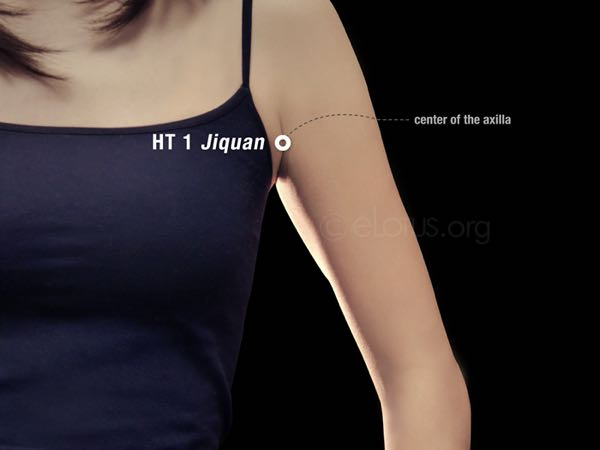
\includegraphics[width=\linewidth]{images/optimized/point_ht1.jpg}\caption{Hình minh họa huyệt HT 1.}\end{figure}
\subsection*{Chỉ định}Đau ở vùng sườn và tim, bìu ; Lạnh và đau ở khuỷu tay và cánh tay; khô cổ họng;
\subsection*{Ứng dụng}Nới lỏng ngực ; Kích hoạt kinh và mang lại lợi ích cho cánh tay;
\subsection*{Thủ thuật}Châm thẳng 0,5-1,0 thốn. Tránh làm thủng động mạch nách.
\subsection*{Phân loại và ghi chú}Điểm đặc biệt Ghi chú: Điểm vào - Tâm
\subsection{HT 2 - Thanh Linh (Qingling)}
\subsection*{Thông tin cơ bản}\begin{description}\item[Hán tự và phiên âm:] 青靈; qīng líng.\item[Ý nghĩa tên (theo tiếng Anh nguồn):] Linh thần xanh (dịch sát nghĩa; literal translation); tiếng Anh nguồn: Cyan Spirit, Green Spirit, Youthful Spirit.\end{description}
\subsection*{Vị trí}Khi khuỷu tay được gấp lại, điểm cao hơn 3 thốn so với đầu trong của nếp gấp ngang [hoặc Thiếu Hải h Tu (HT 3) ], trong rãnh phía trong của cơ nhị đầu cánh tay.
\begin{figure}[H]\centering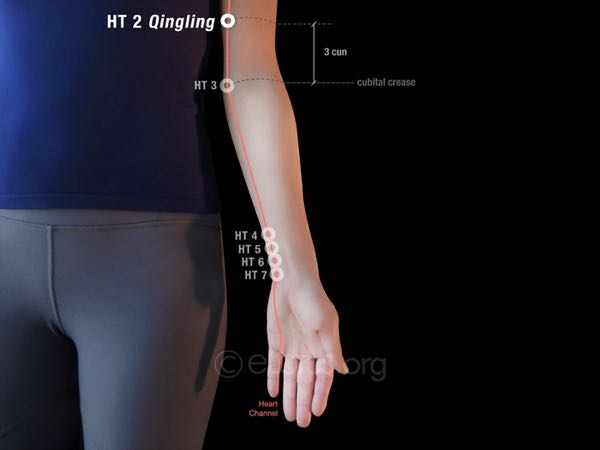
\includegraphics[width=\linewidth]{images/optimized/point_ht2.jpg}\caption{Hình minh họa huyệt HT 2.}\end{figure}
\subsection*{Chỉ định}Tim, vùng hạ sườn, đau vai, cánh tay ;
\subsection*{Ứng dụng}Kích hoạt kinh và giảm bớt cơn đau;
\subsection*{Thủ thuật}Châm thẳng 0,3-0,5 thốn.
\subsection{HT 3 - Thiếu Hải (Shaohai)}
\subsection*{Thông tin cơ bản}\begin{description}\item[Hán tự và phiên âm:] 少海; shào hǎi.\item[Ý nghĩa tên (theo tiếng Anh nguồn):] Biển nhỏ (dịch sát nghĩa; literal translation); tiếng Anh nguồn: Lesser Sea, Lesser Yin Sea.\end{description}
\subsection*{Vị trí}Với khuỷu tay gấp lại, tại điểm giữa của đường nối đầu trong của nếp gấp trụ và mỏm lồi cầu trong của xương cánh tay.
\begin{figure}[H]\centering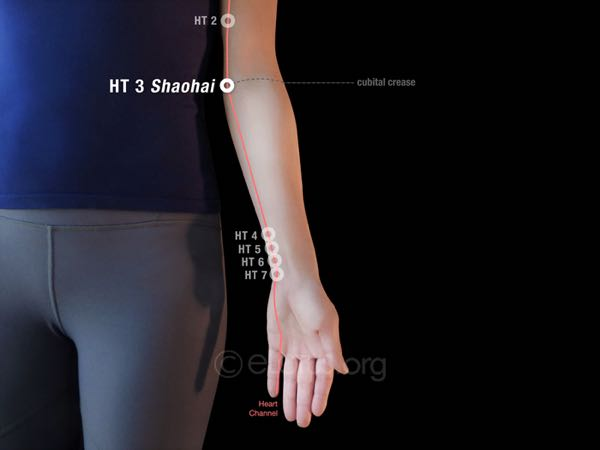
\includegraphics[width=\linewidth]{images/optimized/point_ht3.jpg}\caption{Hình minh họa huyệt HT 3.}\end{figure}
\subsection*{Chỉ định}Đau tim, nách, hạ sườn ; Đau co thắt và tê ở bàn tay và cánh tay, run tay; bìu ;
\subsection*{Ứng dụng}An thần, chuyển đờm và thanh nhiệt; Kích hoạt kinh và mang lại lợi ích cho cánh tay;
\subsection*{Thủ thuật}Châm thẳng 0,5-1,0 thốn.
\subsection*{Phân loại và ghi chú}Điểm đặc biệt nhận xét: He Huyệt Hải (Nước) - Tâm
\subsection{HT 4 - Linh Đạo (Lingdao)}
\subsection*{Thông tin cơ bản}\begin{description}\item[Hán tự và phiên âm:] 靈道; líng dào.\item[Ý nghĩa tên (theo tiếng Anh nguồn):] Đường đi của thần trí (dịch sát nghĩa; literal translation); tiếng Anh nguồn: Spirit Pathway, Mind Path.\end{description}
\subsection*{Vị trí}Với lòng bàn tay hướng lên trên, điểm này nằm ở phía quay của gân cơ gấp cổ tay trụ, cách nếp gấp ngang của cổ tay 1,5 thốn.
\begin{figure}[H]\centering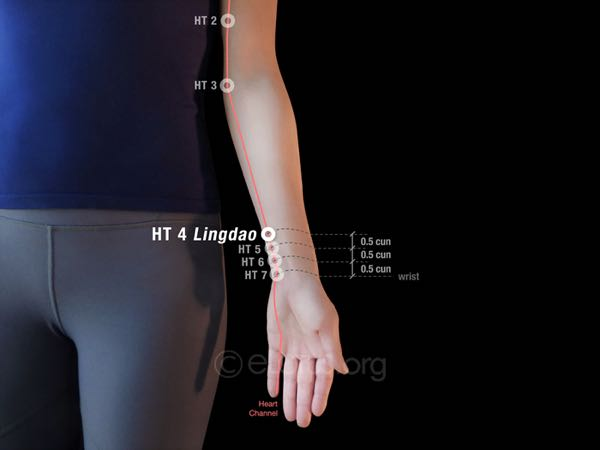
\includegraphics[width=\linewidth]{images/optimized/point_ht4.jpg}\caption{Hình minh họa huyệt HT 4.}\end{figure}
\subsection*{Chỉ định}Đau tim, đau co thắt ở khuỷu tay và cánh tay ; Mất giọng đột ngột;
\subsection*{Ứng dụng}An thần, có lợi cho giọng nói; Thư giãn các cơ và gân;
\subsection*{Thủ thuật}Châm thẳng 0,3-0,5 thốn.
\subsection*{Phân loại và ghi chú}Điểm đặc biệt Ghi chú: Huyệt Kinh (Kim loại) - Tâm
\subsection{HT 5 - Thông Lý (Tongli)}
\subsection*{Thông tin cơ bản}\begin{description}\item[Hán tự và phiên âm:] 通里; tōng lǐ.\item[Ý nghĩa tên (theo tiếng Anh nguồn):] Thông đến bên trong (dịch sát nghĩa; literal translation); tiếng Anh nguồn: Connecting Li, Reaching the Inside, Penetrating the Interior.\end{description}
\subsection*{Vị trí}Với lòng bàn tay hướng lên trên, điểm nằm ở phía quay của gân cơ gấp cổ tay trụ, cách nếp gấp ngang của cổ tay 1 thốn.
\begin{figure}[H]\centering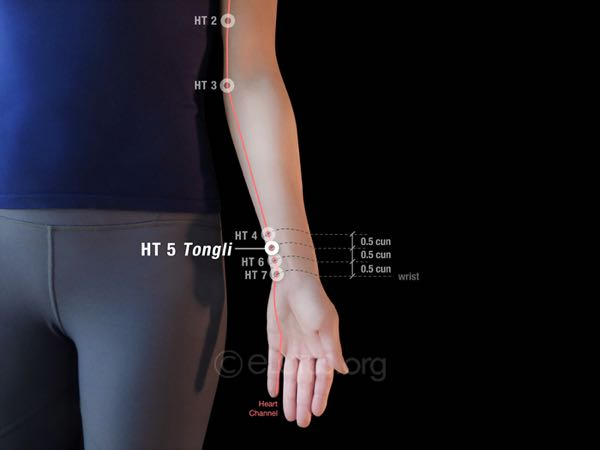
\includegraphics[width=\linewidth]{images/optimized/point_ht5.jpg}\caption{Hình minh họa huyệt HT 5.}\end{figure}
\subsection*{Chỉ định}Đánh trống ngực, chóng mặt, mờ mắt ; Đau họng, mất giọng đột ngột, mất ngôn ngữ kèm cứng lưỡi; Đau ở cổ tay và khuỷu tay;
\subsection*{Ứng dụng}An thần, điều hòa và bồi bổ Tâm ; Lợi ích lưỡi ; Kích hoạt kinh và giảm đau;
\subsection*{Thủ thuật}Châm thẳng 0,3-0,5 thốn.
\subsection*{Phân loại và ghi chú}Điểm đặc biệt Ghi chú: Điểm kết nối Luo - Tâm
\subsection{HT 6 - Âm Khích (Yinxi)}
\subsection*{Thông tin cơ bản}\begin{description}\item[Hán tự và phiên âm:] 陰郄; yīn xī.\item[Ý nghĩa tên (theo tiếng Anh nguồn):] Khe Âm (dịch sát nghĩa; literal translation); tiếng Anh nguồn: Yin Cleft, Yin Accumulation.\end{description}
\subsection*{Vị trí}Với lòng bàn tay hướng lên trên, điểm nằm ở phía quay của gân cơ gấp cổ tay trụ, cao hơn 0,5 thốn so với nếp gấp ngang của cổ tay.
\begin{figure}[H]\centering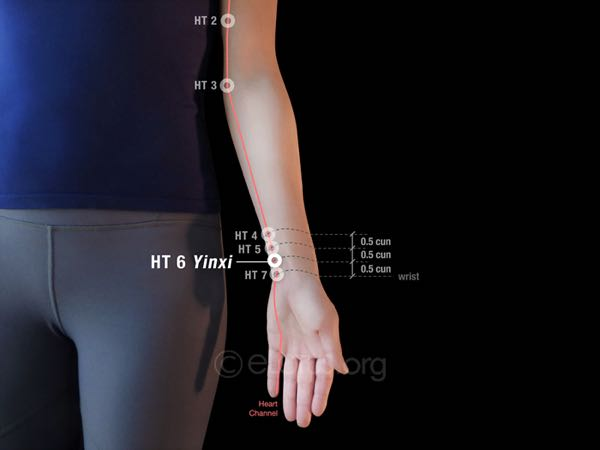
\includegraphics[width=\linewidth]{images/optimized/point_ht6.jpg}\caption{Hình minh họa huyệt HT 6.}\end{figure}
\subsection*{Chỉ định}Đau tim ; Cuồng loạn, mất giọng đột ngột; Đổ mồ hôi đêm, ho ra huyết, chảy huyết cam;
\subsection*{Ứng dụng}Điều hòa huyết mạch, an thần; Điều kiện cấp tính vừa phải; Xóa bỏ lửa thiếu hụt;
\subsection*{Thủ thuật}Châm thẳng 0,3-0,5 thốn.
\subsection*{Phân loại và ghi chú}Điểm đặc biệt Ghi chú: Khích huyệt - Tâm
\subsection{HT 7 - Thần Môn (Shenmen)}
\subsection*{Thông tin cơ bản}\begin{description}\item[Hán tự và phiên âm:] 神門; shén mén.\item[Ý nghĩa tên (theo tiếng Anh nguồn):] Cửa thần trí (dịch sát nghĩa; literal translation); tiếng Anh nguồn: Spirit Gate, Mind Door.\end{description}
\subsection*{Vị trí}Ở đầu trụ của nếp gấp ngang của cổ tay, ở chỗ lõm ở phía quay của gân cơ gấp cổ tay trụ.
\begin{figure}[H]\centering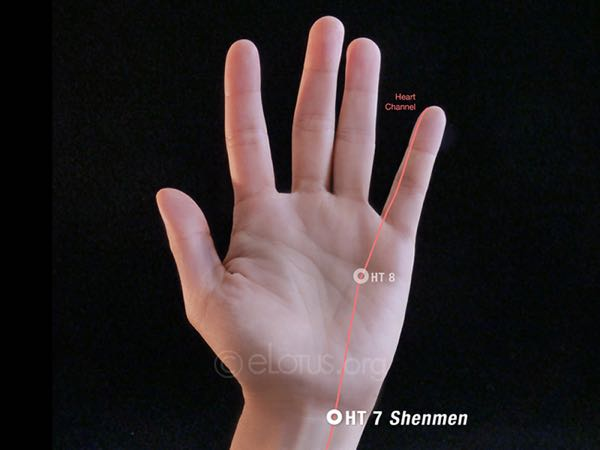
\includegraphics[width=\linewidth]{images/optimized/point_ht7.jpg}\caption{Hình minh họa huyệt HT 7.}\end{figure}
\subsection*{Chỉ định}Cuồng loạn, mất trí nhớ, mất ngủ, hưng cảm, động kinh, mất trí nhớ, khó chịu ; Đau tim, đánh trống ngực; Đau vùng hạ vị, cảm giác sốt ở lòng bàn tay, củng mạc màu vàng;
\subsection*{Ứng dụng}An thần; Điều hòa và làm săn chắc Tâm;
\subsection*{Thủ thuật}Châm thẳng 0,3-0,5 thốn.
\subsection*{Phân loại và ghi chú}Điểm đặc biệt Ghi chú: Điểm suối Shu (Trái đất) - Điểm nguồn Tâm Yuan - Tâm
\subsection{HT 8 - Thiếu Phủ (Shaofu)}
\subsection*{Thông tin cơ bản}\begin{description}\item[Hán tự và phiên âm:] 少府; shào fǔ.\item[Ý nghĩa tên (theo tiếng Anh nguồn):] Dinh nhỏ (dịch sát nghĩa; literal translation); tiếng Anh nguồn: Lesser Mansion, Lesser Yin Mansion, Lesser Palace.\end{description}
\subsection*{Vị trí}Trên lòng bàn tay, ở chỗ lõm giữa xương bàn tay thứ 4 và thứ 5, gần khớp bàn tay. Hoặc khi thực hiện nắm đấm, điểm nằm ở nơi đầu ngón tay út chạm vào lòng bàn tay.
\begin{figure}[H]\centering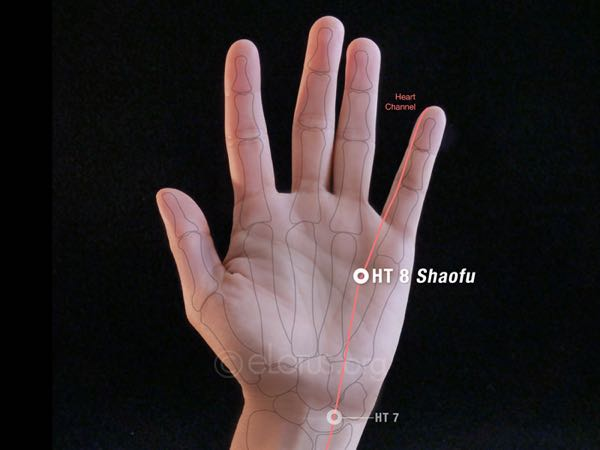
\includegraphics[width=\linewidth]{images/optimized/point_ht8.jpg}\caption{Hình minh họa huyệt HT 8.}\end{figure}
\subsection*{Chỉ định}Đái dầm, tiểu khó, ngứa cơ quan sinh dục ngoài ; Đánh trống ngực, đau ngực; Đau co thắt ở ngón tay út, cảm giác nóng rát ở lòng bàn tay;
\subsection*{Ứng dụng}Thanh nhiệt từ Tâm và Tiểu Trường ; An thần, điều hòa Tâm khí; Kích hoạt kinh và giảm đau;
\subsection*{Thủ thuật}Châm thẳng 0,3-0,5 thốn.
\subsection*{Phân loại và ghi chú}Điểm đặc biệt Ghi chú: Điểm lò xo Ying (Lửa) - Tâm
\subsection{HT 9 - Thiếu Xung (Shaochong)}
\subsection*{Thông tin cơ bản}\begin{description}\item[Hán tự và phiên âm:] 少沖; shào chōng.\item[Ý nghĩa tên (theo tiếng Anh nguồn):] Dòng xung nhỏ (dịch sát nghĩa; literal translation); tiếng Anh nguồn: Lesser Surge, Lesser Rushing, Lesser Yin Rushing.\end{description}
\subsection*{Vị trí}Ở mặt quay của ngón út, cách góc móng khoảng 0,1 thốn.
\begin{figure}[H]\centering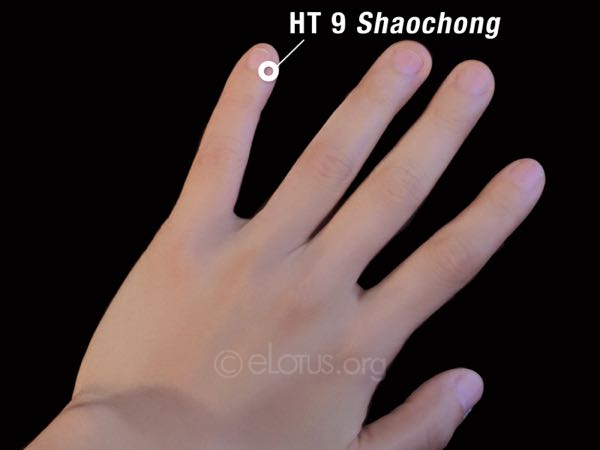
\includegraphics[width=\linewidth]{images/optimized/point_ht9.jpg}\caption{Hình minh họa huyệt HT 9.}\end{figure}
\subsection*{Chỉ định}Đánh trống ngực, đau tim, đau ngực và vùng hạ vị ; Bệnh hưng cảm, sốt, mất ý thức;
\subsection*{Ứng dụng}Phục hồi ý thức; Thanh nhiệt lợi ích lưỡi, mắt, cổ họng; Điều hòa tâm khí và an thần;
\subsection*{Thủ thuật}Châm dưới da 0,1 thốn, hoặc chích nặn máu.
\subsection*{Phân loại và ghi chú}Điểm đặc biệt Ghi chú: Huyệt Tỉnh (Mộc) - Tâm Thoát Điểm - Tâm

\clearpage
\section{Kinh Thủ Thái Dương Tiểu Trường}
\begin{description}
\item[Tên kinh/mạch:] Kinh Thủ Thái Dương Tiểu Trường (Tiểu Trường) .
\item[Hán tự và phiên âm:] 手太陽小腸經; shǒu tài yáng xiǎo cháng jīng.
\item[Thời gian hoạt động:] 1--3 giờ chiều.
\item[Ngũ hành:] Hỏa.
\item[Kinh biểu lý:] Thủ Thiếu Âm Tâm.
\end{description}
\subsection*{Đường đi và phạm vi}Kinh Ruột Nhỏ bắt nguồn từ mặt trụ của đầu ngón tay út, đi dọc theo mặt sau của cánh tay đến khớp vai. Vòng quanh xương bả vai tại Kiên Trinh (SI 9), nó băng qua Phụ Phân (BL 41) và Đại Trữ (BL 11) để gặp Đại Chùy (GV 14) ở phía trên của vai. Sau đó, đi xuống qua vai tới hố thượng đòn, nối với Tâm và đi qua Đản Trung h Tu (CV 17) . Từ đó kinh đi xuống thực quản, đi qua cơ hoành, đến Vị và đi qua Thượng Quản (CV 13) và Trung Quản (CV 12) để đến cơ quan Tiểu Trường. Nhánh từ hố thượng đòn đi lên cổ và xa hơn đến má. Qua khóe ngoài và đi qua Đồng n Tử Liêu (GB 1) và Erheliao (TH 22), kinh đi vào tai tại Thính Cung (SI 19). Nhánh từ cổ chạy lên phía Tuyền Liệu (SI 18) và xa hơn về phía bên của mũi. Sau đó, nó đến khóe mắt bên trong tại Tình Minh (BL 1) để kết nối với kinh Bàng Quang.
\subsection*{Chỉ định của kinh/mạch}Củng mạc mắt có màu vàng, điếc ; Đi tiểu thường xuyên; Sưng má và cổ; Đau dọc theo bờ sau của mặt ngoài vai và cánh tay;
\subsection*{Ứng dụng của kinh/mạch}Kiểm soát việc nhận và chuyển đổi; Tách rõ khỏi đục; Tách chất lỏng;
\subsection*{Phương pháp cân bằng}
\begin{enumerate}
\item Kinh Túc Thái Dương Bàng Quang.
\item Kinh Túc Thái Âm Tỳ.
\item Kinh Thủ Thiếu Âm Tâm.
\item Kinh Túc Quyết Âm Can.
\item Kinh Túc Thái Dương Bàng Quang.
\end{enumerate}
\subsection*{Các huyệt đặc biệt}
\begin{itemize}
\item Tỉnh (Jing-Well): Thiếu Trạch (SI1).
\item Huỳnh (Ying-Spring): Tiền Cốc (SI2).
\item Du (Shu-Stream): Hậu Khê (SI3).
\item Kinh (Jing-River): Dương Cốc (SI5).
\item Hợp (He-Sea): Tiểu Hải (SI8).
\item Nguyên huyệt: Uyển Cốt (SI4).
\item Lạc huyệt: Chi Chính (SI7).
\item Khích huyệt: Dưỡng Lão (SI6).
\item Mộ huyệt trước: Quan Nguyên (CV4).
\item Du huyệt sau: Tiểu Trường Du (BL27).
\item Hạ Hợp huyệt: ST39.
\item Huyệt Mẹ: Hậu Khê (SI3).
\item Huyệt Con: Tiểu Hải (SI8).
\item Huyệt Nhập: Thiếu Trạch (SI1).
\item Huyệt Xuất: Thính Cung (SI19).
\end{itemize}
\subsection{SI 9 - Kiên Trinh (Jianzhen)}
\subsection*{Thông tin cơ bản}\begin{description}\item[Hán tự và phiên âm:] 肩貞; jiān zhēn.\item[Ý nghĩa tên (theo tiếng Anh nguồn):] Vai ngay thẳng (dịch sát nghĩa; literal translation); tiếng Anh nguồn: True Shoulder, Upright Shoulder.\end{description}
\subsection*{Vị trí}Phía sau và dưới khớp vai. Khi khép cánh tay, điểm này cao hơn đầu sau của nếp gấp nách 1 thốn.
\begin{figure}[H]\centering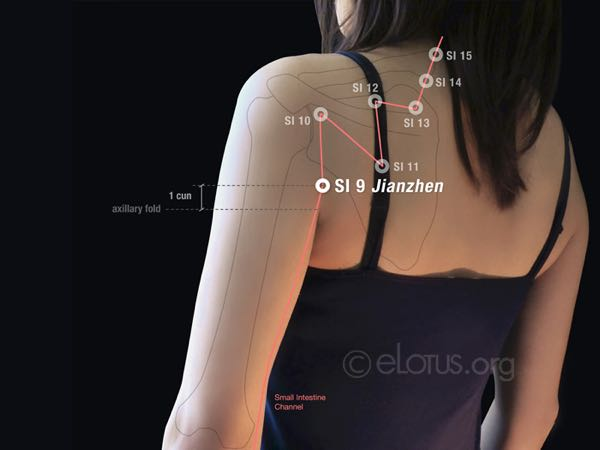
\includegraphics[width=\linewidth]{images/optimized/point_si9.jpg}\caption{Hình minh họa huyệt SI 9.}\end{figure}
\subsection*{Chỉ định}Đau ở vùng xương bả vai ; Suy giảm vận động của bàn tay và cánh tay;
\subsection*{Ứng dụng}Đẩy gió và lợi ích cho vai ; Kích hoạt kinh và giảm đau;
\subsection*{Thủ thuật}Châm thẳng 0,5-1,0 thốn.
\subsection{SI 19 - Thính Cung (Tinggong)}
\subsection*{Thông tin cơ bản}\begin{description}\item[Hán tự và phiên âm:] 聽宮; tīng gōng.\item[Ý nghĩa tên (theo tiếng Anh nguồn):] Cung nghe (dịch sát nghĩa; literal translation); tiếng Anh nguồn: Palace of Hearing, Auditory Palace, Listening Palace.\end{description}
\subsection*{Vị trí}Với miệng mở, điểm này nằm ở chỗ lõm phía trước bình tai và phía sau mỏm lồi cầu của hàm dưới.
\begin{figure}[H]\centering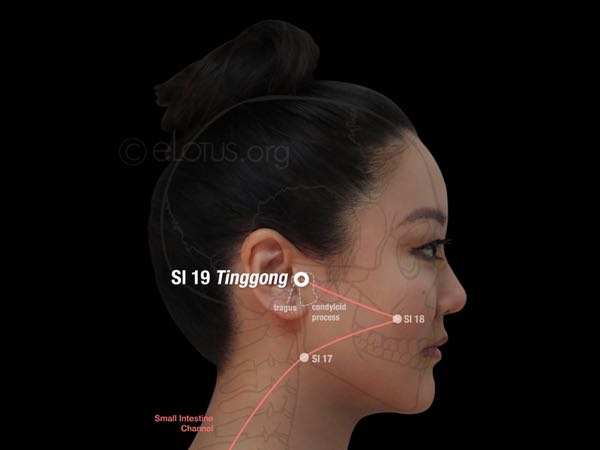
\includegraphics[width=\linewidth]{images/optimized/point_si19.jpg}\caption{Hình minh họa huyệt SI 19.}\end{figure}
\subsection*{Chỉ định}Điếc, ù tai, chảy nước tai ; Suy giảm vận động của khớp hàm dưới; Đau răng;
\subsection*{Ứng dụng}Có lợi cho tai ;
\subsection*{Thủ thuật}Châm thẳng 0,5-1,0 thốn với miệng mở.
\subsection*{Phân loại và ghi chú}Điểm đặc biệt Ghi chú: Điểm thoát - Tiểu Trường
\subsection{SI 18 - Quyền Liêu (Quanliao)}
\subsection*{Thông tin cơ bản}\begin{description}\item[Hán tự và phiên âm:] 顴髎; quán liáo.\item[Ý nghĩa tên (theo tiếng Anh nguồn):] Khe xương gò má (dịch sát nghĩa; literal translation); tiếng Anh nguồn: Cheek Bone Crevice, Cheek Bone Hole, Zygoma Crevice.\end{description}
\subsection*{Vị trí}Ngay bên dưới khóe ngoài, ở chỗ lõm ở bờ dưới của xương gò má.
\begin{figure}[H]\centering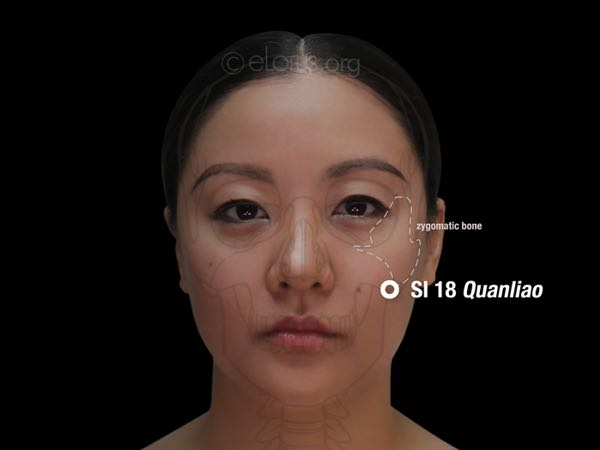
\includegraphics[width=\linewidth]{images/optimized/point_si18.jpg}\caption{Hình minh họa huyệt SI 18.}\end{figure}
\subsection*{Chỉ định}Liệt mặt, co giật mí mắt ; Đau răng, sưng má, đau mặt, củng mạc màu vàng;
\subsection*{Ứng dụng}Khử gió, giảm đau; Thanh nhiệt, giảm sưng tấy;
\subsection*{Thủ thuật}Châm thẳng 0,5-0,8 thốn.
\subsection*{Phân loại và ghi chú}Điểm đặc biệt Ghi chú: Điểm hội tụ kinh tuyến cơ - 3 chân dương
\subsection{SI 1 - Thiếu Trạch (Shaoze)}
\subsection*{Thông tin cơ bản}\begin{description}\item[Hán tự và phiên âm:] 少澤; shào zé.\item[Ý nghĩa tên (theo tiếng Anh nguồn):] Đầm nhỏ (dịch sát nghĩa; literal translation); tiếng Anh nguồn: Lesser Marsh.\end{description}
\subsection*{Vị trí}Ở phía trụ của ngón út, cách góc móng khoảng 0,1 thốn.
\begin{figure}[H]\centering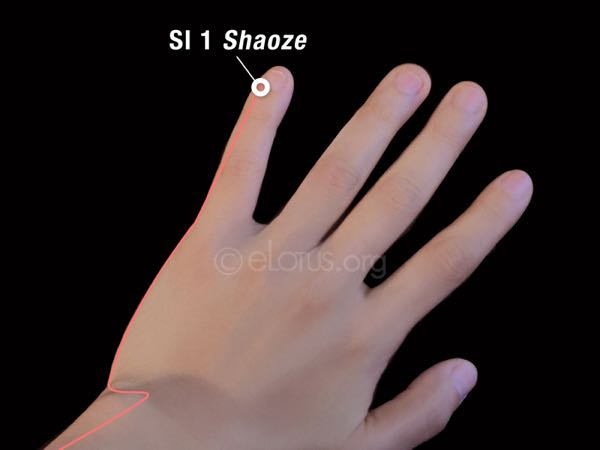
\includegraphics[width=\linewidth]{images/optimized/point_si1.jpg}\caption{Hình minh họa huyệt SI 1.}\end{figure}
\subsection*{Chỉ định}Nhức đầu, các bệnh sốt, đau họng, đỏ mắt, đục giác mạc ; Mất ý thức; Cho con bú không đủ;
\subsection*{Ứng dụng}Thanh nhiệt và có lợi cho các lỗ giác quan ; Phục hồi ý thức; Thúc đẩy quá trình tiết sữa và mang lại lợi ích cho ngực;
\subsection*{Thủ thuật}Châm dưới da 0,1 thốn, hoặc chích nặn máu.
\subsection*{Phân loại và ghi chú}Điểm đặc biệt Ghi chú: Huyệt Tỉnh (Kim loại) - Tiểu Trường Huyệt Nhập - Tiểu Trường
\subsection{SI 2 - Tiền Cốc (Qiangu)}
\subsection*{Thông tin cơ bản}\begin{description}\item[Hán tự và phiên âm:] 前谷; qián gǔ.\item[Ý nghĩa tên (theo tiếng Anh nguồn):] Thung lũng phía trước (dịch sát nghĩa; literal translation); tiếng Anh nguồn: Front Valley.\end{description}
\subsection*{Vị trí}Khi thực hiện động tác nắm tay lỏng lẻo, điểm nằm ở phía trụ của ngón tay út, cách xa khớp đốt ngón tay số 5, tại điểm nối của vùng da đỏ và trắng.
\begin{figure}[H]\centering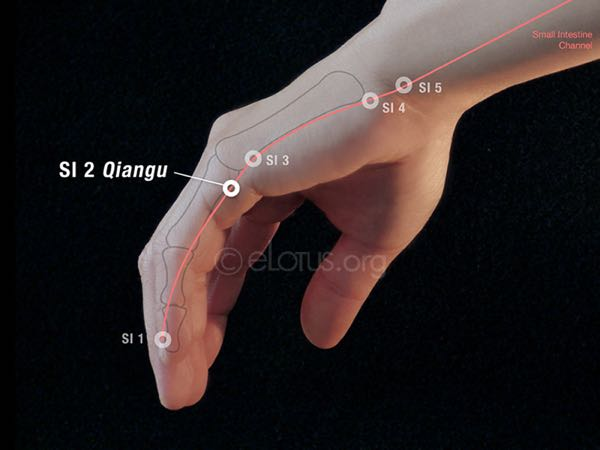
\includegraphics[width=\linewidth]{images/optimized/point_si2.jpg}\caption{Hình minh họa huyệt SI 2.}\end{figure}
\subsection*{Chỉ định}Bệnh sốt, nước tiểu đỏ ; Ù tai, nhức đầu; Tê ngón tay;
\subsection*{Ứng dụng}Làm sạch gió và giảm độ phồng ; Lợi ích cho mắt, tai, họng; Kích hoạt kinh và giảm đau;
\subsection*{Thủ thuật}Châm thẳng 0,3-0,5 thốn.
\subsection*{Phân loại và ghi chú}Điểm đặc biệt Ghi chú: Điểm suối Ying (Nước) - Tiểu Trường
\subsection{SI 3 - Hậu Khê (Houxi)}
\subsection*{Thông tin cơ bản}\begin{description}\item[Hán tự và phiên âm:] 後谿; hòu xī.\item[Ý nghĩa tên (theo tiếng Anh nguồn):] Khe phía sau (dịch sát nghĩa; literal translation); tiếng Anh nguồn: Back Ravine, Back Stream.\end{description}
\subsection*{Vị trí}Khi thực hiện động tác nắm tay lỏng lẻo, điểm nằm ở phía trụ của bàn tay, gần khớp đốt ngón tay thứ 5, tại điểm nối của vùng da đỏ và trắng.
\begin{figure}[H]\centering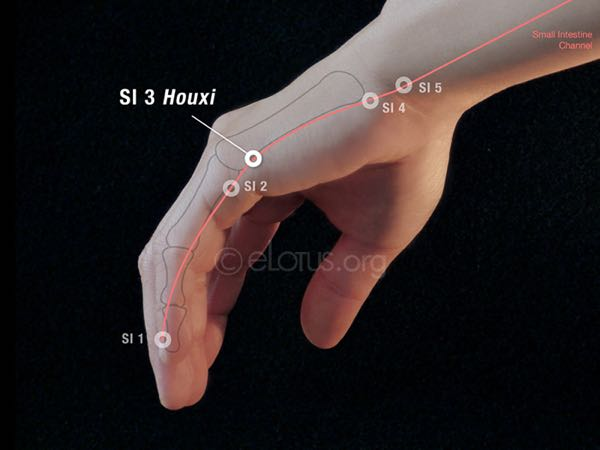
\includegraphics[width=\linewidth]{images/optimized/point_si3.jpg}\caption{Hình minh họa huyệt SI 3.}\end{figure}
\subsection*{Chỉ định}Đau và cứng cổ, vai và khuỷu tay, co rút và tê các ngón tay, bong gân thắt lưng cấp tính ; Đổ mồ hôi đêm, bệnh sốt, viêm họng, sốt rét; Ù tai, điếc; Hưng cảm, động kinh;
\subsection*{Ứng dụng}Có lợi cho vùng chẩm, cổ và lưng; Kích hoạt kinh và giảm đau; Làm sạch gió và nhiệt; An thần; Lợi ích các lỗ giác quan; Điều chỉnh kinh du (quản lý);
\subsection*{Thủ thuật}Châm thẳng 0,5-0,7 thốn.
\subsection*{Phân loại và ghi chú}Điểm đặc biệt Ghi chú: Điểm suối Shu (Mộc) - Điểm chủ Tiểu Trường - Kinh Du (Chi phối) Điểm ghép - Kinh Yangqiao (Chuyển động)
\subsection{SI 4 - Uyển Cốt (Wangu)}
\subsection*{Thông tin cơ bản}\begin{description}\item[Hán tự và phiên âm:] 腕骨; wàn gǔ.\item[Ý nghĩa tên (theo tiếng Anh nguồn):] Xương cổ tay (dịch sát nghĩa; literal translation); tiếng Anh nguồn: Wrist Bone.\end{description}
\subsection*{Vị trí}Ở phía trụ của bàn tay, ở chỗ lõm giữa gốc xương bàn ngón thứ 5 và xương hamate.
\begin{figure}[H]\centering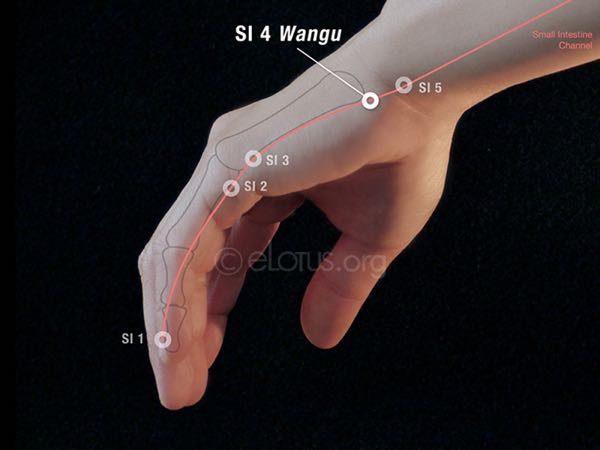
\includegraphics[width=\linewidth]{images/optimized/point_si4.jpg}\caption{Hình minh họa huyệt SI 4.}\end{figure}
\subsection*{Chỉ định}Co rút các ngón tay, đau cổ tay ; Đau đầu, cứng cổ; Các bệnh sốt kèm theo bệnh khan tiết mồ hôi, vàng da;
\subsection*{Ứng dụng}Kích hoạt kinh và giảm bớt cơn đau; Thanh nhiệt và giảm sưng tấy; Xóa ẩm ướt;
\subsection*{Thủ thuật}Châm thẳng 0,3-0,5 thốn.
\subsection*{Phân loại và ghi chú}Điểm đặc biệt Ghi chú: Điểm nguồn Yuan - Tiểu Trường
\subsection{SI 5 - Dương Cốc (Yanggu)}
\subsection*{Thông tin cơ bản}\begin{description}\item[Hán tự và phiên âm:] 陽谷; yáng gǔ.\item[Ý nghĩa tên (theo tiếng Anh nguồn):] Thung lũng Dương (dịch sát nghĩa; literal translation); tiếng Anh nguồn: Yang Valley.\end{description}
\subsection*{Vị trí}Ở đầu trụ của nếp gấp ngang ở mặt sau của cổ tay, ở chỗ lõm giữa mỏm trâm của xương trụ và xương ba que.
\begin{figure}[H]\centering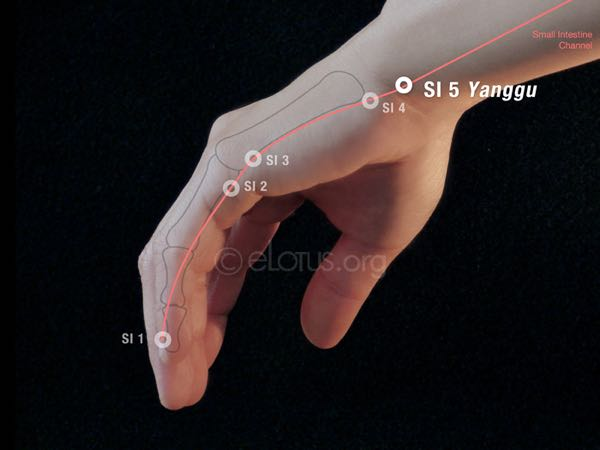
\includegraphics[width=\linewidth]{images/optimized/point_si5.jpg}\caption{Hình minh họa huyệt SI 5.}\end{figure}
\subsection*{Chỉ định}Sưng cổ và vùng dưới hàm ; Đau tay, cổ tay; Bệnh sốt;
\subsection*{Ứng dụng}Thanh nhiệt và giảm sưng tấy ; An thần;
\subsection*{Thủ thuật}Châm thẳng 0,3-0,5 thốn.
\subsection*{Phân loại và ghi chú}Điểm đặc biệt Ghi chú: Huyệt Kinh (Lửa) - Tiểu Trường
\subsection{SI 6 - Dưỡng Lão (Yanglao)}
\subsection*{Thông tin cơ bản}\begin{description}\item[Hán tự và phiên âm:] 養老; yǎng lǎo.\item[Ý nghĩa tên (theo tiếng Anh nguồn):] Nuôi dưỡng người già (dịch sát nghĩa; literal translation); tiếng Anh nguồn: Nursing the Aged, Support the Aged,  Nourish ing the Old.\end{description}
\subsection*{Vị trí}Với lòng bàn tay hướng về phía ngực, điểm này nằm ở mặt sau của đầu xương trụ, trong khe xương ở phía quay của mỏm trâm của xương trụ.
\begin{figure}[H]\centering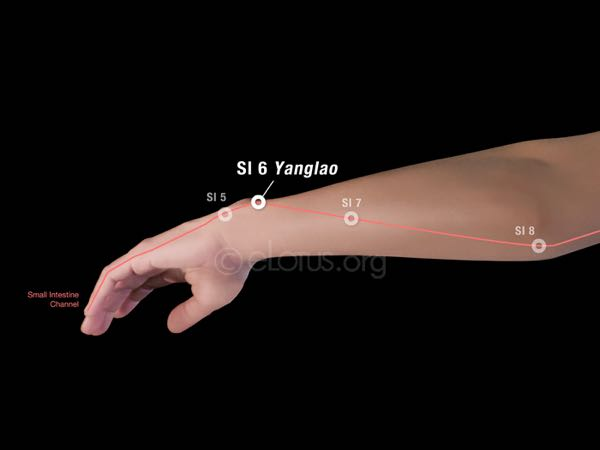
\includegraphics[width=\linewidth]{images/optimized/point_si6.jpg}\caption{Hình minh họa huyệt SI 6.}\end{figure}
\subsection*{Chỉ định}Đau vai, khuỷu tay, cánh tay ; Làm mờ tầm nhìn;
\subsection*{Ứng dụng}Kích hoạt kinh và giảm đau, mang lại lợi ích cho vai và cánh tay; Điều kiện cấp tính vừa phải; Lợi ích cho mắt;
\subsection*{Thủ thuật}Châm thẳng 0,3-0,5 thốn.
\subsection*{Phân loại và ghi chú}Điểm đặc biệt Ghi chú: Khích huyệt - Tiểu Trường
\subsection{SI 7 - Chi Chính (Zhizheng)}
\subsection*{Thông tin cơ bản}\begin{description}\item[Hán tự và phiên âm:] 支正; zhī zhèng.\item[Ý nghĩa tên (theo tiếng Anh nguồn):] Nhánh của sự ngay thẳng (dịch sát nghĩa; literal translation); tiếng Anh nguồn: Branch of Upright, Branch to the Correct.\end{description}
\subsection*{Vị trí}Nằm trên đường nối Dương Cốc (SI 5) và Tiểu Hải M (SI 8), cách nếp gấp mặt lưng của cổ tay 5 thốn, trong rãnh giữa bờ trước của xương trụ và cơ gấp carpi ulnaris.
\begin{figure}[H]\centering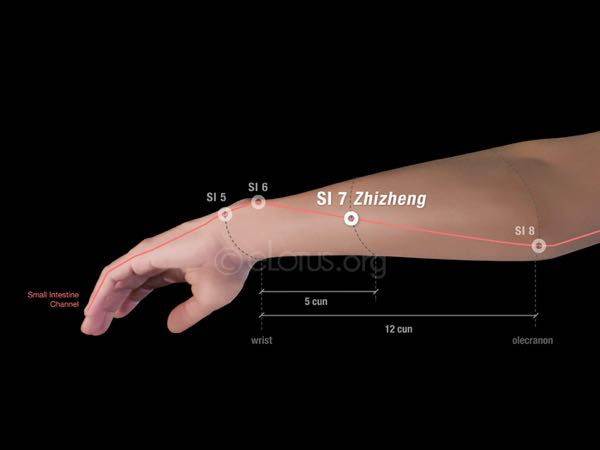
\includegraphics[width=\linewidth]{images/optimized/point_si7.jpg}\caption{Hình minh họa huyệt SI 7.}\end{figure}
\subsection*{Chỉ định}Cổ cứng, nhức đầu, chóng mặt, các bệnh sốt ; hưng cảm ; Đau co thắt ở khuỷu tay và ngón tay;
\subsection*{Ứng dụng}Làm sạch nhiệt và giải phóng bên ngoài ; An thần; Kích hoạt kinh và giảm đau, có lợi cho khớp ngón tay;
\subsection*{Thủ thuật}Châm thẳng 0,5-0,8 thốn.
\subsection*{Phân loại và ghi chú}Điểm đặc biệt Ghi chú: Điểm kết nối Luo - Tiểu Trường
\subsection{SI 8 - Tiểu Hải (Xiaohai)}
\subsection*{Thông tin cơ bản}\begin{description}\item[Hán tự và phiên âm:] 小海; xiǎo hǎi.\item[Ý nghĩa tên (theo tiếng Anh nguồn):] Biển nhỏ (dịch sát nghĩa; literal translation); tiếng Anh nguồn: Small Sea.\end{description}
\subsection*{Vị trí}Với khuỷu tay gấp, điểm này nằm ở chỗ lõm giữa mỏm khuỷu của xương trụ và mỏm lồi cầu trong của xương cánh tay.
\begin{figure}[H]\centering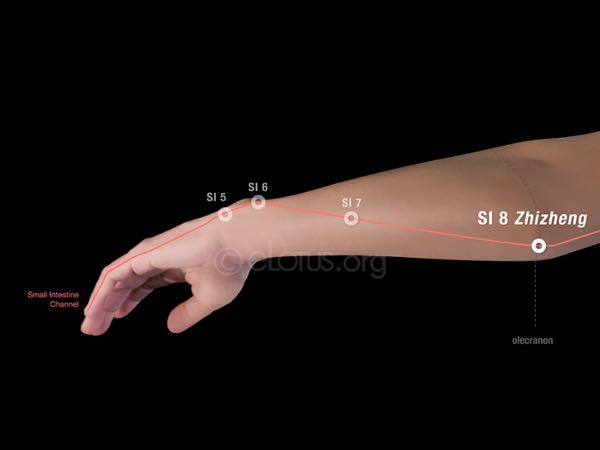
\includegraphics[width=\linewidth]{images/optimized/point_si8.jpg}\caption{Hình minh họa huyệt SI 8.}\end{figure}
\subsection*{Chỉ định}Nhức đầu, sưng má ; Chóng mặt, động kinh; Đau vùng gáy, vai, cánh tay và khuỷu tay;
\subsection*{Ứng dụng}Thanh nhiệt và tiêu sưng tấy; An thần; Kích hoạt kinh và giảm đau;
\subsection*{Thủ thuật}Châm thẳng 0,3-0,5 thốn.
\subsection*{Phân loại và ghi chú}Điểm đặc biệt nhận xét: He Huyệt Hải (Trái đất) - Tiểu Trường
\subsection{SI 10 - Nhu Du (Naoshu)}
\subsection*{Thông tin cơ bản}\begin{description}\item[Hán tự và phiên âm:] 臑俞; nāo shū.\item[Ý nghĩa tên (theo tiếng Anh nguồn):] Hốc xương cánh tay trên (dịch sát nghĩa; literal translation); tiếng Anh nguồn: Upper arm transporter, Upper Arm Shu.\end{description}
\subsection*{Vị trí}Khi khép cánh tay, điểm này nằm ngay phía trên đầu sau của nếp nách, ở chỗ lõm phía dưới cột sống vai.
\begin{figure}[H]\centering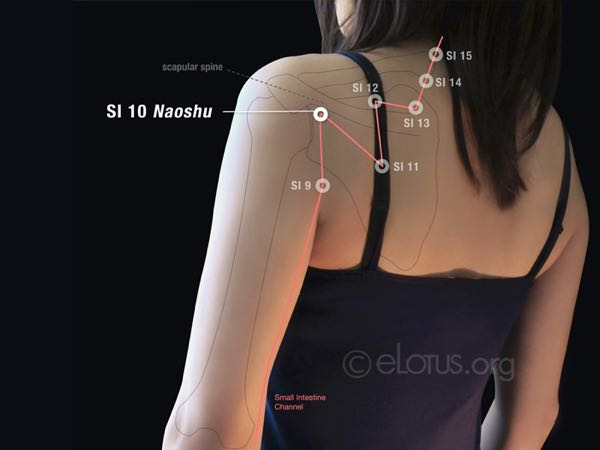
\includegraphics[width=\linewidth]{images/optimized/point_si10.jpg}\caption{Hình minh họa huyệt SI 10.}\end{figure}
\subsection*{Chỉ định}Sưng vai, đau nhức và yếu vai và cánh tay ;
\subsection*{Ứng dụng}Kích hoạt kinh và giảm đau, có lợi cho vai ;
\subsection*{Thủ thuật}Châm thẳng 0,5-1,0 thốn.
\subsection{SI 11 - Thiên Tông (Tianzong)}
\subsection*{Thông tin cơ bản}\begin{description}\item[Hán tự và phiên âm:] 天宗; tiān zōng.\item[Ý nghĩa tên (theo tiếng Anh nguồn):] Sự hội tụ trên trời (dịch sát nghĩa; literal translation); tiếng Anh nguồn: Heavenly Gathering, Celestial Gathering, Heavenly Attribution.\end{description}
\subsection*{Vị trí}Trên xương bả vai, ở chỗ lõm ở trung tâm hố dưới gai, ngang mức đốt sống ngực thứ 4.
\begin{figure}[H]\centering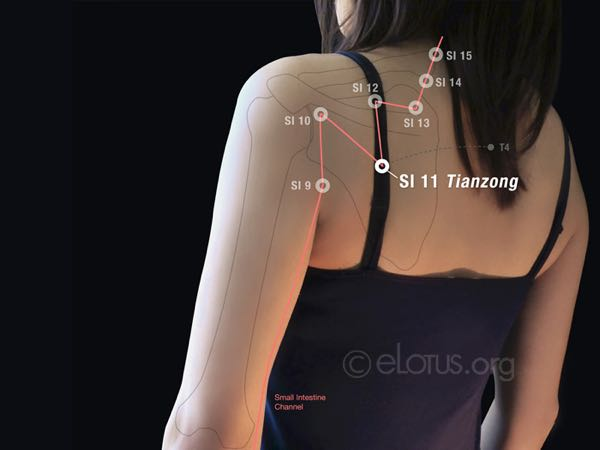
\includegraphics[width=\linewidth]{images/optimized/point_si11.jpg}\caption{Hình minh họa huyệt SI 11.}\end{figure}
\subsection*{Chỉ định}Đau ở vùng xương bả vai ; Đau ở mặt sau của khuỷu tay và cánh tay; hen suyễn;
\subsection*{Ứng dụng}Kích hoạt kinh và giảm bớt cơn đau; Vận chuyển khí và làm lỏng vùng ngực và vùng sườn bên;
\subsection*{Thủ thuật}Châm thẳng hoặc xiên 0,5-1,0 thốn.
\subsection{SI 12 - Bỉnh Phong (Bingfeng)}
\subsection*{Thông tin cơ bản}\begin{description}\item[Hán tự và phiên âm:] 秉風; bǐng fēng.\item[Ý nghĩa tên (theo tiếng Anh nguồn):] Nắm bắt gió (dịch sát nghĩa; literal translation); tiếng Anh nguồn: Grasping the Wind.\end{description}
\subsection*{Vị trí}Ở trung tâm của hố trên xương bả vai, ngay phía trên Thiên Tông (SI 11) . Khi cánh tay được nâng lên, điểm nằm ở chỗ lõm.
\begin{figure}[H]\centering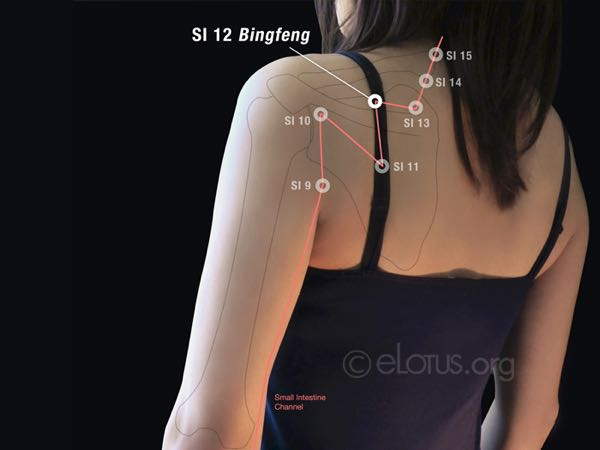
\includegraphics[width=\linewidth]{images/optimized/point_si12.jpg}\caption{Hình minh họa huyệt SI 12.}\end{figure}
\subsection*{Chỉ định}Đau ở vùng xương bả vai ; Tê và đau nhức các chi trên, suy giảm khả năng vận động của vai và cánh tay;
\subsection*{Ứng dụng}Đẩy gió, lợi ích cho vai và xương bả vai;
\subsection*{Thủ thuật}Châm thẳng 0,5-0,7 thốn.
\subsection{SI 13 - Khúc Viên (Quyuan)}
\subsection*{Thông tin cơ bản}\begin{description}\item[Hán tự và phiên âm:] 曲垣; qū yuán.\item[Ý nghĩa tên (theo tiếng Anh nguồn):] Bức tường cong (dịch sát nghĩa; literal translation); tiếng Anh nguồn: Crooked Wall, Bend Wall.\end{description}
\subsection*{Vị trí}Trong chỗ lõm ở đầu trong của hố trên bả vai, nằm giữa Nhu Du (SI 10) và mỏm gai của T2.
\begin{figure}[H]\centering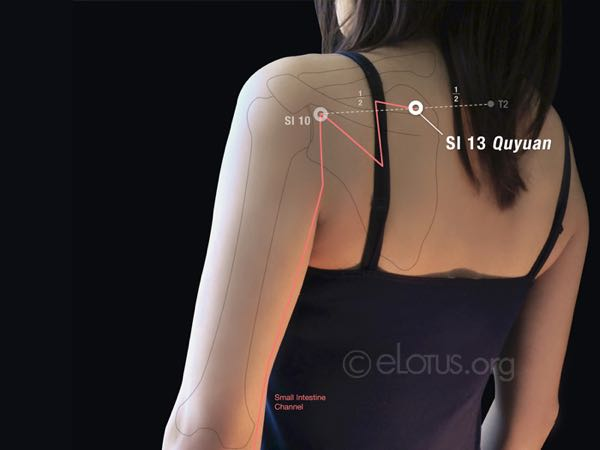
\includegraphics[width=\linewidth]{images/optimized/point_si13.jpg}\caption{Hình minh họa huyệt SI 13.}\end{figure}
\subsection*{Chỉ định}Đau và cứng vùng xương bả vai ;
\subsection*{Ứng dụng}Có lợi cho vai và xương bả vai ;
\subsection*{Thủ thuật}Châm thẳng 0,3-0,5 thốn.
\subsection{SI 14 - Kiên Ngoại Du (Jianwaishu)}
\subsection*{Thông tin cơ bản}\begin{description}\item[Hán tự và phiên âm:] 肩外俞; jiān wài shū.\item[Ý nghĩa tên (theo tiếng Anh nguồn):] Du huyệt ngoài vai (dịch sát nghĩa; literal translation); tiếng Anh nguồn: Outer Shoulder Transporter, Outer Shoulder Shu.\end{description}
\subsection*{Vị trí}3 thốn về phía bờ dưới của mỏm gai T1 [Đào Đạo m.yd (GV 13) ].
\begin{figure}[H]\centering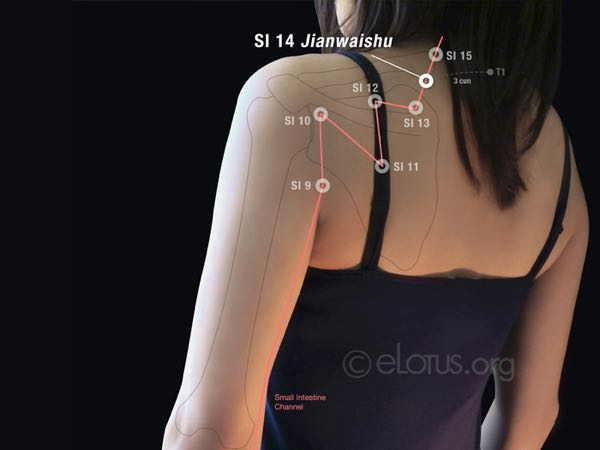
\includegraphics[width=\linewidth]{images/optimized/point_si14.jpg}\caption{Hình minh họa huyệt SI 14.}\end{figure}
\subsection*{Chỉ định}Đau vai và lưng ; Đau và cứng cổ;
\subsection*{Ứng dụng}Kích hoạt kinh và giảm bớt cơn đau; Đẩy gió lạnh, lợi ích vai và xương bả vai;
\subsection*{Thủ thuật}Châm xiên 0,3-0,7 thốn.
\subsection{SI 15 - Kiên Trung Du (Jianzhongshu)}
\subsection*{Thông tin cơ bản}\begin{description}\item[Hán tự và phiên âm:] 肩中俞; jiān zhōng shū.\item[Ý nghĩa tên (theo tiếng Anh nguồn):] Du huyệt giữa vai (dịch sát nghĩa; literal translation); tiếng Anh nguồn: Middle Shoulder Transporter, Middle Shoulder Shu.\end{description}
\subsection*{Vị trí}2 thốn bên tính đến bờ dưới của mỏm gai C7 [Đại Chùy (GV 14) ].
\begin{figure}[H]\centering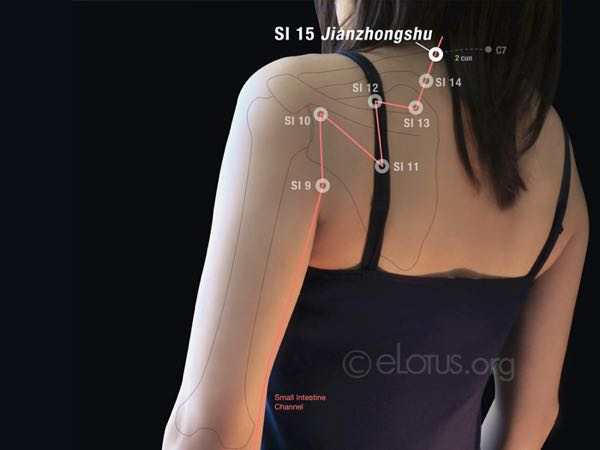
\includegraphics[width=\linewidth]{images/optimized/point_si15.jpg}\caption{Hình minh họa huyệt SI 15.}\end{figure}
\subsection*{Chỉ định}Ho, hen suyễn, ho ra huyết ; Đau ở vai và lưng;
\subsection*{Ứng dụng}đi xuống khí Phế ; Kích hoạt kinh và giảm đau;
\subsection*{Thủ thuật}Châm xiên 0,3-0,6 thốn.
\subsection{SI 16 - Thiên Song (Tianchuang)}
\subsection*{Thông tin cơ bản}\begin{description}\item[Hán tự và phiên âm:] 天窗; tiān chuāng.\item[Ý nghĩa tên (theo tiếng Anh nguồn):] Cửa sổ trời (dịch sát nghĩa; literal translation); tiếng Anh nguồn: Heavenly Window, Celestial Window.\end{description}
\subsection*{Vị trí}Ở phía bên cổ, phía sau cơ ức đòn chũm, ngang với đỉnh quả táo Adam.
\begin{figure}[H]\centering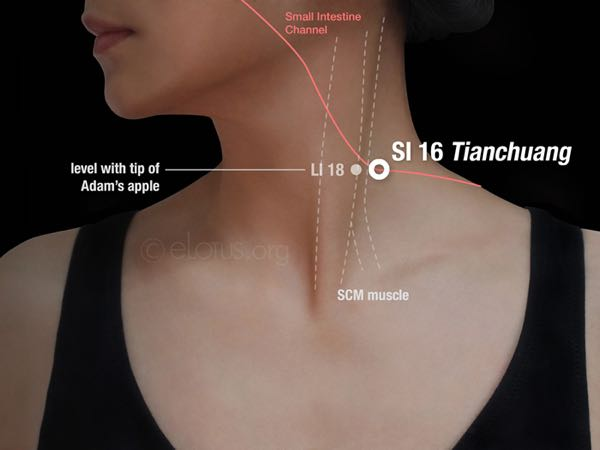
\includegraphics[width=\linewidth]{images/optimized/point_si16.jpg}\caption{Hình minh họa huyệt SI 16.}\end{figure}
\subsection*{Chỉ định}Đau họng, mất giọng đột ngột, điếc, ù tai ; Cổ cứng và đau;
\subsection*{Ứng dụng}Có lợi cho tai, họng, giọng nói; Điều hòa khí và an thần; Kích hoạt kinh mạch, giảm đau, thanh nhiệt;
\subsection*{Thủ thuật}Châm thẳng 0,3-0,7 thốn. Điểm đặc biệt của
\subsection*{Phân loại và ghi chú}Ghi chú: Cửa sổ Sky Point
\subsection{SI 17 - Thiên Dung (Tianrong)}
\subsection*{Thông tin cơ bản}\begin{description}\item[Hán tự và phiên âm:] 天容; tiān róng.\item[Ý nghĩa tên (theo tiếng Anh nguồn):] Dung mạo trên trời (dịch sát nghĩa; literal translation); tiếng Anh nguồn: Heavenly Appearance, Celestial Countenance.\end{description}
\subsection*{Vị trí}Phía sau góc hàm dưới, trong chỗ lõm ở bờ trước của cơ ức đòn chũm.
\begin{figure}[H]\centering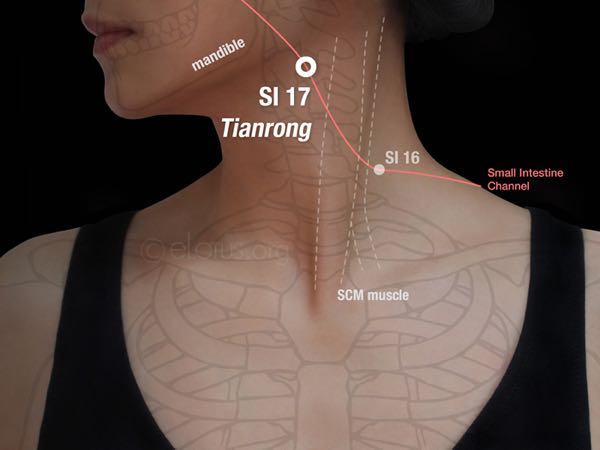
\includegraphics[width=\linewidth]{images/optimized/point_si17.jpg}\caption{Hình minh họa huyệt SI 17.}\end{figure}
\subsection*{Chỉ định}Đau họng, sưng má ; Cảm giác có dị vật trong họng, bướu cổ; Điếc, ù tai;
\subsection*{Ứng dụng}Có lợi cho cổ và cổ họng và làm giảm sưng tấy ; Khí phản loạn giáng xuống; Lợi ích cho tai;
\subsection*{Thủ thuật}Châm thẳng 0,5-0,7 thốn. Điểm đặc biệt của
\subsection*{Phân loại và ghi chú}Ghi chú: Cửa sổ Sky Point

\clearpage
\section{Kinh Túc Thái Dương Bàng Quang}
\begin{description}
\item[Tên kinh/mạch:] Kinh Túc Thái Dương Bàng Quang (Bàng Quang) .
\item[Hán tự và phiên âm:] 足太陽膀胱經; zú tài yáng páng guāng jīng.
\item[Thời gian hoạt động:] 3--5 giờ chiều.
\item[Ngũ hành:] Thủy.
\item[Kinh biểu lý:] Túc Thiếu Âm Thận.
\end{description}
\subsection*{Đường đi và phạm vi}Kinh Bàng Quang tiết niệu bắt nguồn từ khóe trong tại Tình Minh (BL 1), đi lên trán về phía Thần Đình (GV 24) và Đầu Lâm Khấp (GB 15), sau đó đi lên đỉnh đầu về phía Bách Hội (GV 20) nơi có một nhánh phát sinh, chạy đến chùa và băng qua Khúc Tân (GB 7) qua Hoàn Cốt (GB 12) . Nhánh thẳng đi vào não, sau đó đi xuống dọc theo mặt sau của cổ, băng qua Não Hộ (GV 17) , hướng về Thiên Trụ (BL 10) . Sau đó nó băng qua Đại Chùy (GV 14) và Đào Đạo m.yd (GV 13) để đi qua Đại Trữ (BL 11) và đi xuống Uỷ Trung (BL 40), đi vào cơ quan Thận và cơ quan Bàng Quang trên đường đi. Nhánh vùng thắt lưng đi xuống qua vùng mông và kết thúc ở hố khoeo. Nhánh từ mặt sau của cổ chạy thẳng xuống dọc theo bờ trong của xương bả vai từ Phụ Phân (BL 41), băng qua Hoàn Khiêu (GB 30) , xuống Chí Âm (BL 67), nơi nó kết nối với kinh Thận.
\subsection*{Chỉ định của kinh/mạch}Bí tiểu, đái dầm ; Đau vùng gáy, phần trên và phần dưới của lưng, mặt sau của chi dưới; Sốt rét; Đau mắt;
\subsection*{Ứng dụng của kinh/mạch}Loại bỏ nước bằng cách chuyển đổi Khí; Lưu trữ nước tiểu tạm thời;
\subsection*{Phương pháp cân bằng}
\begin{enumerate}
\item Kinh Thủ Thái Dương Tiểu Trường.
\item Kinh Thủ Thái Âm Phế.
\item Kinh Túc Thiếu Âm Thận.
\item Kinh Thủ Thái Âm Phế.
\item Kinh Thủ Thái Dương Tiểu Trường.
\end{enumerate}
\subsection*{Các huyệt đặc biệt}
\begin{itemize}
\item Tỉnh (Jing-Well): Chí Âm (BL67).
\item Huỳnh (Ying-Spring): Túc Thông Cốc (BL66).
\item Du (Shu-Stream): Thúc Cốt (BL65).
\item Kinh (Jing-River): Côn Lôn (BL60).
\item Hợp (He-Sea): Uỷ Trung (BL40).
\item Nguyên huyệt: Kinh Cốt (BL64).
\item Lạc huyệt: Phi Dương (BL58).
\item Khích huyệt: Kim Môn (BL63).
\item Mộ huyệt trước: Trung Cực (CV3).
\item Du huyệt sau: Bàng Quang Du (BL28).
\item Hạ Hợp huyệt: Uỷ Trung (BL40).
\item Huyệt Mẹ: Chí Âm (BL67).
\item Huyệt Con: Thúc Cốt (BL65).
\item Huyệt Nhập: Tình Minh (BL1).
\item Huyệt Xuất: Chí Âm (BL67).
\end{itemize}
\subsection{BL 1 - Tình Minh (Jingming)}
\subsection*{Thông tin cơ bản}\begin{description}\item[Hán tự và phiên âm:] 睛明; jīng míng.\item[Ý nghĩa tên (theo tiếng Anh nguồn):] Mắt sáng (dịch sát nghĩa; literal translation); tiếng Anh nguồn: Bright Eyes, Eye Brightness.\end{description}
\subsection*{Vị trí}Ở chỗ lõm phía trên một chút (khoảng 0,1 thốn ở phía trong và phía trên) khóe mắt bên trong.
\begin{figure}[H]\centering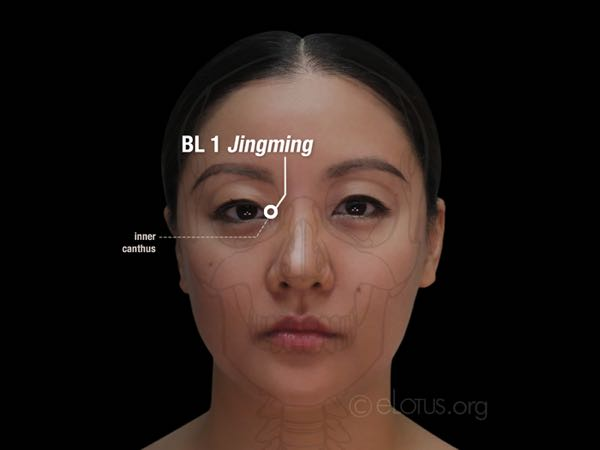
\includegraphics[width=\linewidth]{images/optimized/point_bl1.jpg}\caption{Hình minh họa huyệt BL 1.}\end{figure}
\subsection*{Chỉ định}Đỏ, sưng, đau mắt, ngứa khóe mắt, chảy nước mắt ; Quáng gà, mù màu, nhìn mờ, cận thị;
\subsection*{Ứng dụng}Có lợi cho mắt; Đẩy gió và thanh nhiệt;
\subsection*{Thủ thuật}Khi bệnh nhân nhắm mắt, nhẹ nhàng đẩy nhãn cầu về phía bên. Châm từ từ, thẳng 0,3-0,7 thốn dọc theo thành ổ mắt để tránh nhãn cầu. Không nên vặn hoặc nhấc và đẩy mạnh kim. Để tránh chảy huyết, hãy ấn vào vị trí châm thủng trong vài giây sau khi rút kim.
\subsection*{Phân loại và ghi chú}Điểm đặc biệt Ghi chú: Điểm vào - Bàng Quang
\subsection{BL 10 - Thiên Trụ (Tianzhu)}
\subsection*{Thông tin cơ bản}\begin{description}\item[Hán tự và phiên âm:] 天柱; tiān zhù.\item[Ý nghĩa tên (theo tiếng Anh nguồn):] Cột trời (dịch sát nghĩa; literal translation); tiếng Anh nguồn: Celestial Pillar, Heavenly Pillar.\end{description}
\subsection*{Vị trí}Ở mặt ngoài của cơ thang, cách đường giữa 1,3 thốn [Á Môn (GV 15) ].
\begin{figure}[H]\centering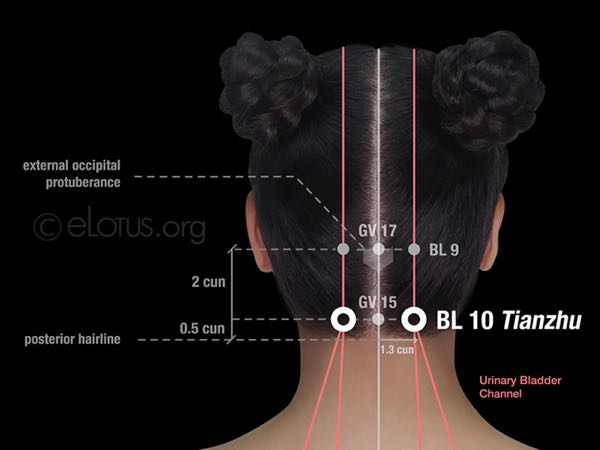
\includegraphics[width=\linewidth]{images/optimized/point_bl10.jpg}\caption{Hình minh họa huyệt BL 10.}\end{figure}
\subsection*{Chỉ định}Nhức đầu, cứng cổ, đau vai và lưng ; Nghẹt mũi, đau họng;
\subsection*{Ứng dụng}Điều hòa khí và tiêu tán gió ; Có lợi cho đầu và các lỗ giác quan; An thần; Kích hoạt kinh và giảm đau;
\subsection*{Thủ thuật}Châm thẳng 0,5-0,8 thốn. Điểm đặc biệt của
\subsection*{Phân loại và ghi chú}Ghi chú: Cửa sổ Sky Point
\subsection{BL 11 - Đại Trữ (Dazhu)}
\subsection*{Thông tin cơ bản}\begin{description}\item[Hán tự và phiên âm:] 大杼; dà zhù.\item[Ý nghĩa tên (theo tiếng Anh nguồn):] Cái guồng lớn (dịch sát nghĩa; literal translation); tiếng Anh nguồn: Great Shuttle, Big Reed.\end{description}
\subsection*{Vị trí}1,5 thốn bên tính đến bờ dưới của mỏm gai T1 [Đào Đạo m.yd (GV 13) ].
\begin{figure}[H]\centering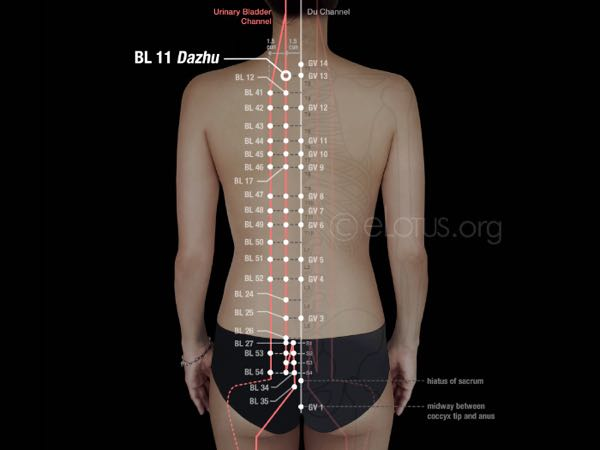
\includegraphics[width=\linewidth]{images/optimized/point_bl11.jpg}\caption{Hình minh họa huyệt BL 11.}\end{figure}
\subsection*{Chỉ định}Nhức đầu, đau cổ và lưng, cứng cổ, đau và nhức ở vùng xương bả vai ; Ho, sốt;
\subsection*{Ứng dụng}Có lợi cho xương khớp; Trục xuất các yếu tố gây bệnh và tăng cường khí công (phòng thủ); Điều hòa Phế khí;
\subsection*{Thủ thuật}Châm xiên 0,5-0,7 thốn. Không nên đặt vuông góc vì nó có thể gây tràn khí màng Phế.
\subsection*{Phân loại và ghi chú}Điểm Đặc Biệt Ghi Chú: 8 Điểm Ảnh Hưởng - Xương 4 Điểm Biển - huyết
\subsection{BL 40 - Uỷ Trung (Weizhong)}
\subsection*{Thông tin cơ bản}\begin{description}\item[Hán tự và phiên âm:] 委中; wěi zhōng.\item[Ý nghĩa tên (theo tiếng Anh nguồn):] Ở giữa chỗ khoeo (dịch sát nghĩa; literal translation); tiếng Anh nguồn: Bend Middle, Middle of the Crook, Supporting the Middle.\end{description}
\subsection*{Vị trí}Điểm giữa của nếp gấp khoeo, giữa các gân của cơ nhị đầu đùi và cơ bán gân.
\begin{figure}[H]\centering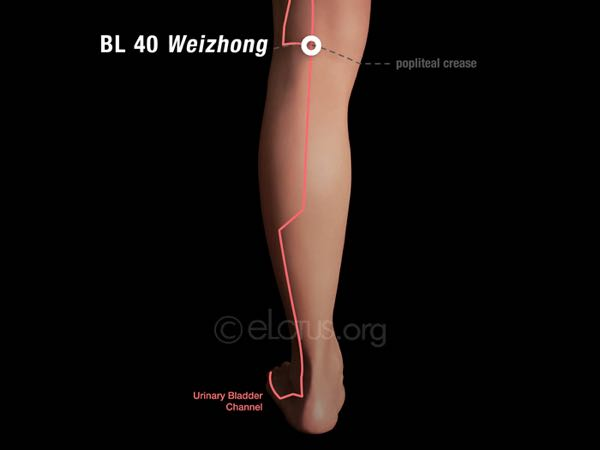
\includegraphics[width=\linewidth]{images/optimized/point_bl40.jpg}\caption{Hình minh họa huyệt BL 40.}\end{figure}
\subsection*{Chỉ định}Đau lưng dưới, suy giảm vận động khớp hông ; Teo cơ, đau, tê, suy giảm vận động chi dưới, co rút gân ở hố khoeo; Liệt nửa người, viêm quầng ; Đau bụng, nôn mửa, tiêu chảy;
\subsection*{Ứng dụng}Có lợi cho vùng thắt lưng và đầu gối; Kích hoạt kinh và giảm đau; Làm mát huyết, thanh nhiệt mùa hè;
\subsection*{Thủ thuật}Châm thẳng 0,5-1,0 thốn, hoặc chích vào tĩnh mạch khoeo để chảy huyết.
\subsection*{Phân loại và ghi chú}Điểm đặc biệt Ghi chú: He Huyệt Hải (Trái đất) - Bàng Quang Hạ He Huyệt Hải - Bàng Quang Command Point - Back (Trên và Dưới)
\subsection{BL 41 - Phụ Phân (Fufen)}
\subsection*{Thông tin cơ bản}\begin{description}\item[Hán tự và phiên âm:] 附分; fù fēn.\item[Ý nghĩa tên (theo tiếng Anh nguồn):] Nhánh phụ gắn kèm (dịch sát nghĩa; literal translation); tiếng Anh nguồn: Attached Branch, Appended Part.\end{description}
\subsection*{Vị trí}3 thốn về phía ngoài so với đường giữa, ngang với bờ dưới của mỏm gai T2 và Phong Môn (BL 12), trên bờ cột sống của xương bả vai.
\begin{figure}[H]\centering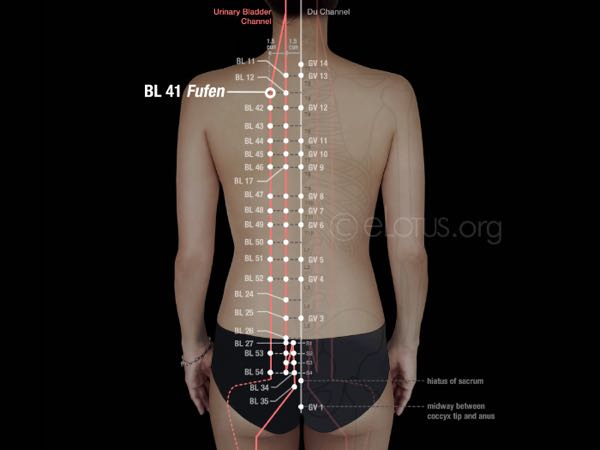
\includegraphics[width=\linewidth]{images/optimized/point_bl41.jpg}\caption{Hình minh họa huyệt BL 41.}\end{figure}
\subsection*{Chỉ định}Cứng khớp, đau vai, lưng và cổ ; Tê khuỷu tay và cánh tay;
\subsection*{Ứng dụng}Kích hoạt kinh và giảm bớt cơn đau; Khu phong và lạnh;
\subsection*{Thủ thuật}Châm xiên 0,3-0,5 thốn. Không nên đặt vuông góc vì nó có thể gây tràn khí màng Phế.
\subsection{BL 67 - Chí Âm (Zhiyin)}
\subsection*{Thông tin cơ bản}\begin{description}\item[Hán tự và phiên âm:] 至陰; zhì yīn.\item[Ý nghĩa tên (theo tiếng Anh nguồn):] Đạt đến Âm (dịch sát nghĩa; literal translation); tiếng Anh nguồn: Reaching Yin.\end{description}
\subsection*{Vị trí}Ở mặt bên của ngón chân cái, cách góc móng khoảng 0,1 thốn.
\begin{figure}[H]\centering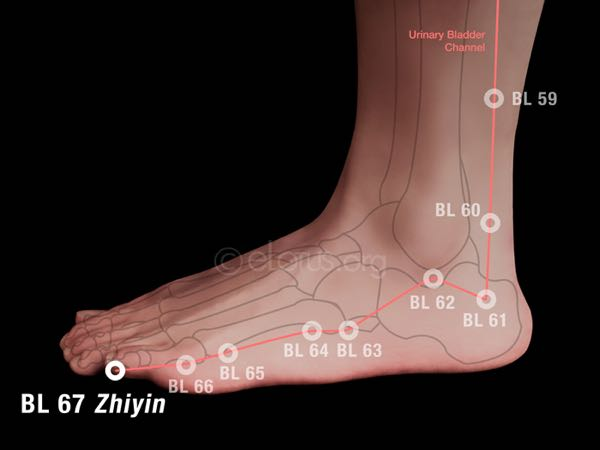
\includegraphics[width=\linewidth]{images/optimized/point_bl67.jpg}\caption{Hình minh họa huyệt BL 67.}\end{figure}
\subsection*{Chỉ định}Nhức đầu, đau mắt, nghẹt mũi, chảy huyết cam ; Thai nhi sai vị trí, chuyển dạ khó khăn, nhau thai ứ đọng; Cảm giác sốt ở lòng bàn chân;
\subsection*{Ứng dụng}Xua gió, thông thoáng đầu óc ; Xoay bào thai, tạo điều kiện chuyển dạ;
\subsection*{Thủ thuật}Châm nông 0,1 thốn, hoặc chích nặn máu.
\subsection*{Phân loại và ghi chú}Điểm đặc biệt Ghi chú: Huyệt Tỉnh (Kim loại) - Bàng Quang Huyệt Xuất - Bàng Quang
\subsection{BL 2 - Toản Trúc (Zanzhu)}
\subsection*{Thông tin cơ bản}\begin{description}\item[Hán tự và phiên âm:] 攢竹; zán zhú.\item[Ý nghĩa tên (theo tiếng Anh nguồn):] Trúc tụ (dịch sát nghĩa; literal translation); tiếng Anh nguồn: Bamboo Gathering, Gathered Bamboo.\end{description}
\subsection*{Vị trí}Trong chỗ lõm ở đầu trong của lông mày, phía trên khóe mắt bên trong hoặc trên rãnh trên ổ mắt.
\begin{figure}[H]\centering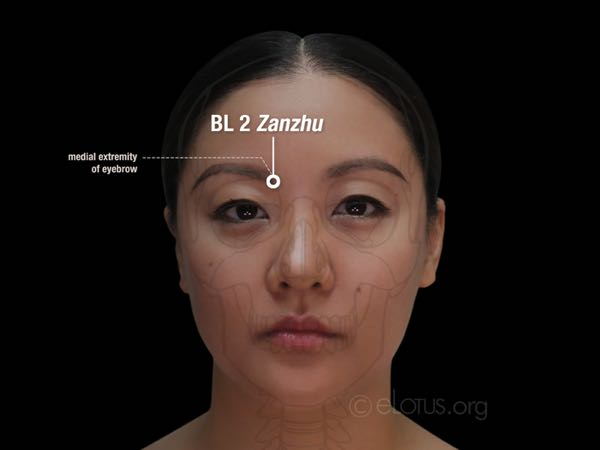
\includegraphics[width=\linewidth]{images/optimized/point_bl2.jpg}\caption{Hình minh họa huyệt BL 2.}\end{figure}
\subsection*{Chỉ định}Đỏ, sưng và đau mắt, co giật mí mắt ; Mờ và suy giảm thị lực, tăng nhãn áp, chảy nước mắt; Nhức đầu, đau vùng trên ổ mắt;
\subsection*{Ứng dụng}Khử gió và thanh nhiệt ; Lợi ích cho mắt; Làm sạch đầu và giảm đau;
\subsection*{Thủ thuật}Châm dưới da 0,3-0,5 thốn, hoặc chích nặn máu.
\subsection{BL 3 - My Xung (Meichong)}
\subsection*{Thông tin cơ bản}\begin{description}\item[Hán tự và phiên âm:] 眉衝; méi chōng.\item[Ý nghĩa tên (theo tiếng Anh nguồn):] Mày xung (dịch sát nghĩa; literal translation); tiếng Anh nguồn: Eyebrow Ascension, Eyebrow's Rushing, Eyebrow's Pouring.\end{description}
\subsection*{Vị trí}Ngay phía trên Toản Trúc h Tu (BL 2) , 0,5 thốn trong đường chân tóc phía trước, ngang với Thần Đình (GV 24) .
\begin{figure}[H]\centering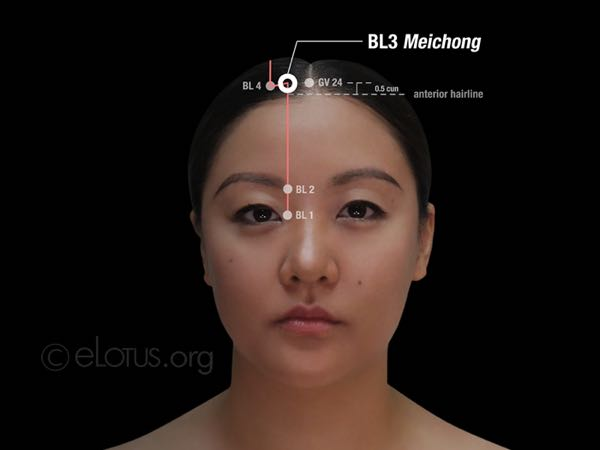
\includegraphics[width=\linewidth]{images/optimized/point_bl3.jpg}\caption{Hình minh họa huyệt BL 3.}\end{figure}
\subsection*{Chỉ định}Nhức đầu, chóng mặt, động kinh ; Nghẹt mũi;
\subsection*{Ứng dụng}Đẩy gió, làm đầu óc tỉnh táo và giảm đau; Lợi ích cho mắt và mũi;
\subsection*{Thủ thuật}Châm dưới da 0,3-0,5 thốn.
\subsection{BL 4 - Khúc Sai (Quchai)}
\subsection*{Thông tin cơ bản}\begin{description}\item[Hán tự và phiên âm:] 曲差; qǔ chāi.\item[Ý nghĩa tên (theo tiếng Anh nguồn):] Khúc quanh lệch (dịch sát nghĩa; literal translation); tiếng Anh nguồn: Deviating Turn, Crooked Curve, Discrepancy.\end{description}
\subsection*{Vị trí}0,5 thốn trong đường chân tóc phía trước, 1,5 thốn về phía sau so với đường giữa [Thần Đình (GV 24) ], tại điểm giao nhau của 1/3 trong và 2/3 bên của khoảng cách từ Thần Đình (GV 24) đến Đầu Duy (ST 8) .
\begin{figure}[H]\centering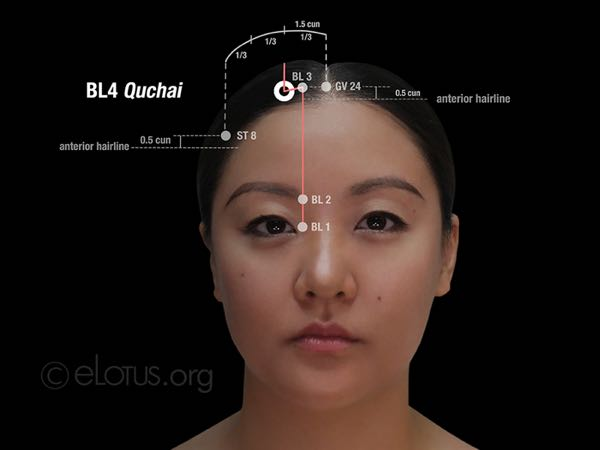
\includegraphics[width=\linewidth]{images/optimized/point_bl4.jpg}\caption{Hình minh họa huyệt BL 4.}\end{figure}
\subsection*{Chỉ định}Đau đầu ; Nghẹt mũi, chảy huyết cam; Nhìn mờ, giảm thị lực;
\subsection*{Ứng dụng}Xua gió, làm đầu óc tỉnh táo, giảm đau; Lợi ích cho mắt và mũi;
\subsection*{Thủ thuật}Châm dưới da 0,3-0,5 thốn.
\subsection{BL 5 - Ngũ Xứ (Wuchu)}
\subsection*{Thông tin cơ bản}\begin{description}\item[Hán tự và phiên âm:] 五處; wǔ chǔ.\item[Ý nghĩa tên (theo tiếng Anh nguồn):] Nơi thứ năm (dịch sát nghĩa; literal translation); tiếng Anh nguồn: Fifth Place, Five Places.\end{description}
\subsection*{Vị trí}1 thốn trong chân tóc phía trước, 1,5 thốn bên trong đường giữa [Thượng Tinh (GV 23) ].
\begin{figure}[H]\centering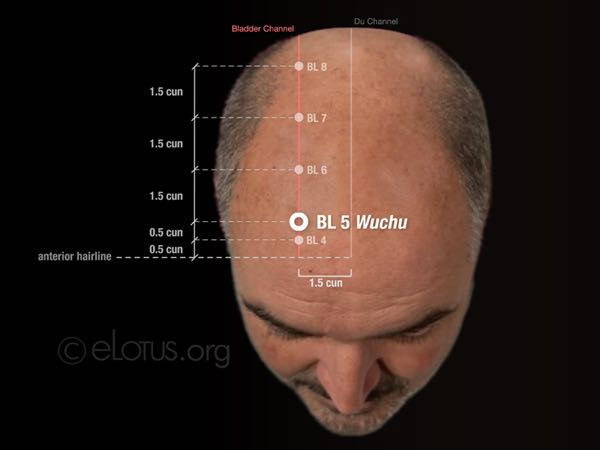
\includegraphics[width=\linewidth]{images/optimized/point_bl5.jpg}\caption{Hình minh họa huyệt BL 5.}\end{figure}
\subsection*{Chỉ định}Động kinh, co giật ; Đau đầu, mờ mắt;
\subsection*{Ứng dụng}Khử gió, hạ dương, thanh nhiệt ; Làm sạch đầu và mũi;
\subsection*{Thủ thuật}Châm dưới da 0,3-0,5 thốn.
\subsection{BL 6 - Thừa Quang (Chengguang)}
\subsection*{Thông tin cơ bản}\begin{description}\item[Hán tự và phiên âm:] 承光; chéng guāng.\item[Ý nghĩa tên (theo tiếng Anh nguồn):] Tiếp nhận ánh sáng (dịch sát nghĩa; literal translation); tiếng Anh nguồn: Light Guard, Support Light, Receiving Light.\end{description}
\subsection*{Vị trí}2,5 thốn trong đường chân tóc phía trước hoặc 1,5 thốn phía sau so với Ngũ Xứ (BL 5), 1,5 thốn phía sau đường giữa.
\begin{figure}[H]\centering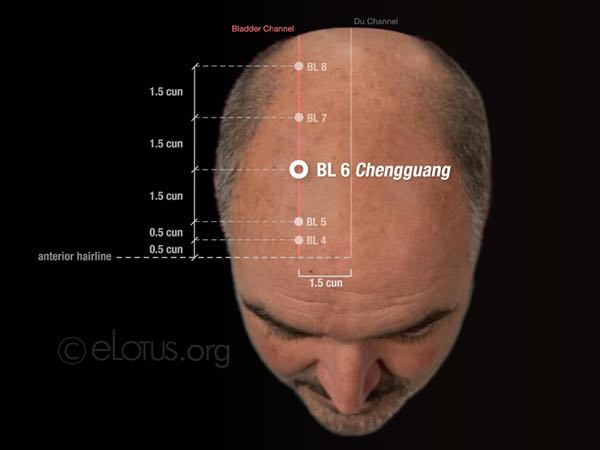
\includegraphics[width=\linewidth]{images/optimized/point_bl6.jpg}\caption{Hình minh họa huyệt BL 6.}\end{figure}
\subsection*{Chỉ định}Nhức đầu, mờ mắt, nghẹt mũi ;
\subsection*{Ứng dụng}Khử gió và thanh nhiệt ; Làm sạch đầu, có lợi cho mắt và mũi;
\subsection*{Thủ thuật}Châm dưới da 0,3-0,5 thốn.
\subsection{BL 7 - Thông Thiên (Tongtian)}
\subsection*{Thông tin cơ bản}\begin{description}\item[Hán tự và phiên âm:] 通天; tōng tiān.\item[Ý nghĩa tên (theo tiếng Anh nguồn):] Thông lên trời (dịch sát nghĩa; literal translation); tiếng Anh nguồn: Celestial Connection, Reaching Heaven, Heavenly Connection.\end{description}
\subsection*{Vị trí}4 thốn trong đường chân tóc phía trước hoặc 1,5 thốn phía sau tính đến Thừa Quang (BL 6), 1,5 thốn phía sau đường giữa.
\begin{figure}[H]\centering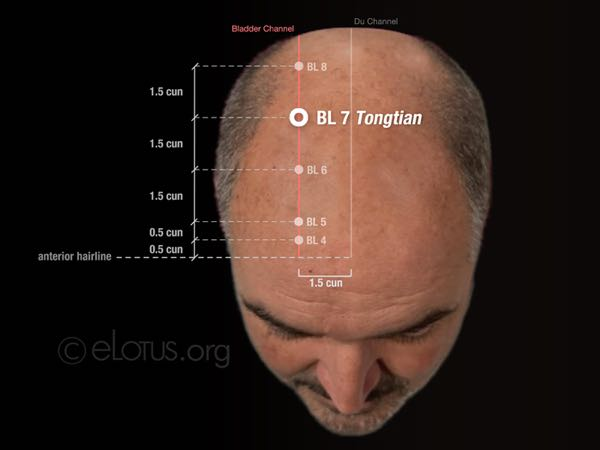
\includegraphics[width=\linewidth]{images/optimized/point_bl7.jpg}\caption{Hình minh họa huyệt BL 7.}\end{figure}
\subsection*{Chỉ định}Nghẹt mũi, chảy huyết cam, chảy nước mũi ; Đau đầu ;
\subsection*{Ứng dụng}Lợi ích và điều hòa mũi ; Làm sạch đầu;
\subsection*{Thủ thuật}Châm dưới da 0,3-0,5 thốn.
\subsection{BL 8 - Lạc Khước (Luoque)}
\subsection*{Thông tin cơ bản}\begin{description}\item[Hán tự và phiên âm:] 絡卻; luò què.\item[Ý nghĩa tên (theo tiếng Anh nguồn):] Liên kết suy giảm (dịch sát nghĩa; literal translation); tiếng Anh nguồn: Declining Connection.\end{description}
\subsection*{Vị trí}5,5 thốn trong đường chân tóc phía trước hoặc 1,5 thốn phía sau tính từ Thông Điền (BL 7), 1,5 thốn ở phía ngoài đường giữa.
\begin{figure}[H]\centering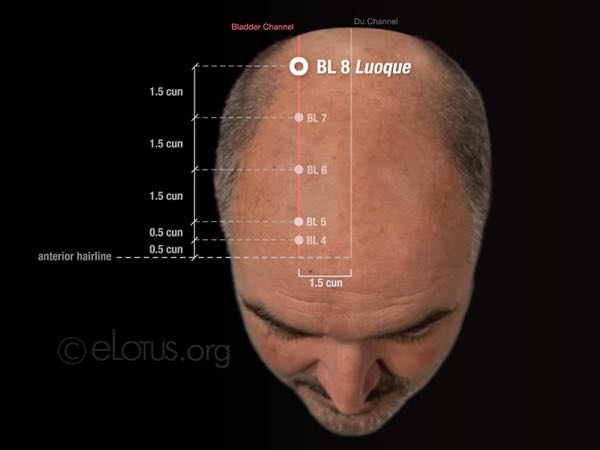
\includegraphics[width=\linewidth]{images/optimized/point_bl8.jpg}\caption{Hình minh họa huyệt BL 8.}\end{figure}
\subsection*{Chỉ định}Chóng mặt, mờ mắt, ù tai ; hưng cảm ;
\subsection*{Ứng dụng}Có lợi cho các giác quan; Xua tan gió, hóa đờm, an thần;
\subsection*{Thủ thuật}Châm dưới da 0,3-0,5 thốn.
\subsection{BL 9 - Ngọc Chẩm (Yuzhen)}
\subsection*{Thông tin cơ bản}\begin{description}\item[Hán tự và phiên âm:] 玉枕; yù zhěn.\item[Ý nghĩa tên (theo tiếng Anh nguồn):] Gối ngọc (dịch sát nghĩa; literal translation); tiếng Anh nguồn: Jade Pillow.\end{description}
\subsection*{Vị trí}2,5 thốn trong chân tóc sau, 1,3 thốn phía ngoài đường giữa [Não Hộ (GV 17) ], ở chỗ lõm phía trên chẩm bên ngoài.
\begin{figure}[H]\centering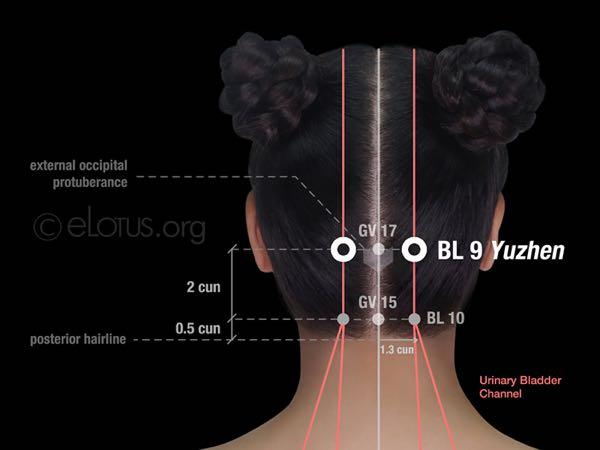
\includegraphics[width=\linewidth]{images/optimized/point_bl9.jpg}\caption{Hình minh họa huyệt BL 9.}\end{figure}
\subsection*{Chỉ định}Nhức đầu, đau cổ, chóng mặt ; Nghẹt mũi; Đau mắt;
\subsection*{Ứng dụng}Xua gió lạnh, giảm đau; Thông mũi và mắt;
\subsection*{Thủ thuật}Châm dưới da 0,3-0,5 thốn.
\subsection{BL 12 - Phong Môn (Fengmen)}
\subsection*{Thông tin cơ bản}\begin{description}\item[Hán tự và phiên âm:] 風門; fēng mén.\item[Ý nghĩa tên (theo tiếng Anh nguồn):] Cửa gió (dịch sát nghĩa; literal translation); tiếng Anh nguồn: Wind Gate, Wind Door.\end{description}
\subsection*{Vị trí}cách bờ dưới của mỏm gai T2 1,5 thốn.
\begin{figure}[H]\centering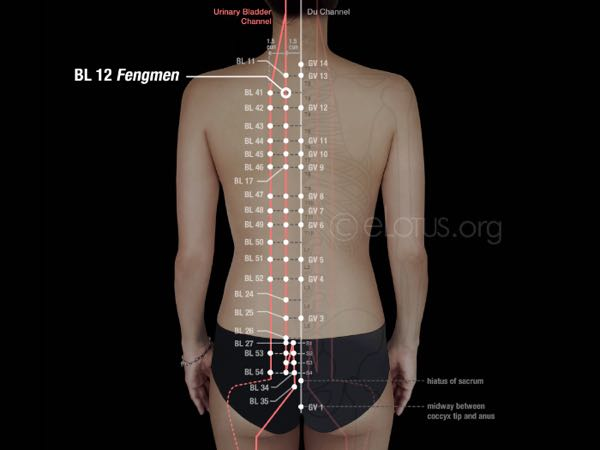
\includegraphics[width=\linewidth]{images/optimized/point_bl12.jpg}\caption{Hình minh họa huyệt BL 12.}\end{figure}
\subsection*{Chỉ định}Cảm lạnh, ho, sốt thông thường; Đau đầu, cứng cổ, đau lưng;
\subsection*{Ứng dụng}Trục xuất gió và giải phóng bên ngoài, tăng cường khí công (phòng thủ); Phổ biến và đi xuống Phế khí;
\subsection*{Thủ thuật}Châm xiên 0,5-0,7 thốn. Không nên đặt vuông góc vì nó có thể gây tràn khí màng Phế.
\subsection{BL 13 - Phế Du (Feishu)}
\subsection*{Thông tin cơ bản}\begin{description}\item[Hán tự và phiên âm:] 肺俞; fèi shū.\item[Ý nghĩa tên (theo tiếng Anh nguồn):] Du huyệt Phế (dịch sát nghĩa; literal translation); tiếng Anh nguồn: Lung Shu, Lung Back Transporting Point.\end{description}
\subsection*{Vị trí}1,5 thốn bên tính đến bờ dưới của mỏm gai T3 [Thân Trụ (GV 12) ].
\begin{figure}[H]\centering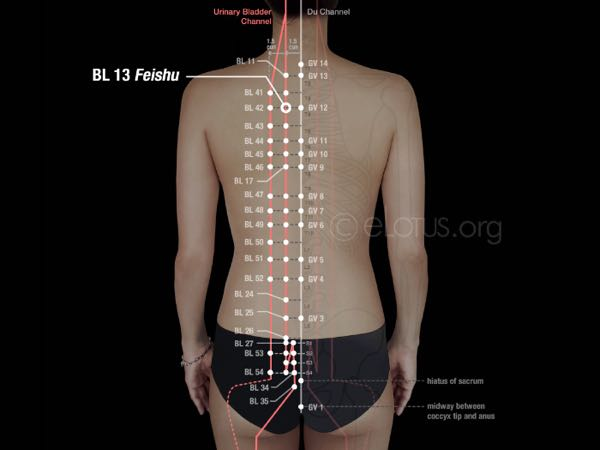
\includegraphics[width=\linewidth]{images/optimized/point_bl13.jpg}\caption{Hình minh họa huyệt BL 13.}\end{figure}
\subsection*{Chỉ định}Sốt chiều, đổ mồ hôi đêm ; Ho, hen suyễn, đau ngực; Khạc ra huyết;
\subsection*{Ứng dụng}Tăng cường khí Phế, nuôi dưỡng âm Phế; Đi xuống, phổ biến khí Phế, thanh nhiệt Phế; Giải phóng bên ngoài;
\subsection*{Thủ thuật}Châm xiên 0,5-0,7 thốn. Không nên đặt vuông góc vì nó có thể gây tràn khí màng Phế.
\subsection*{Phân loại và ghi chú}Phân loại và ghi chú: Điểm quay lại Shu - Phế
\subsection{BL 14 - Quyết Âm Du (Jueyinshu)}
\subsection*{Thông tin cơ bản}\begin{description}\item[Hán tự và phiên âm:] 厥陰俞; jué yīn shū.\item[Ý nghĩa tên (theo tiếng Anh nguồn):] Du huyệt Quyết Âm (dịch sát nghĩa; literal translation); tiếng Anh nguồn: Jue Yin Shu, Terminal Yin Back Transporting Point.\end{description}
\subsection*{Vị trí}cách bờ dưới của mỏm gai T4 1,5 thốn.
\begin{figure}[H]\centering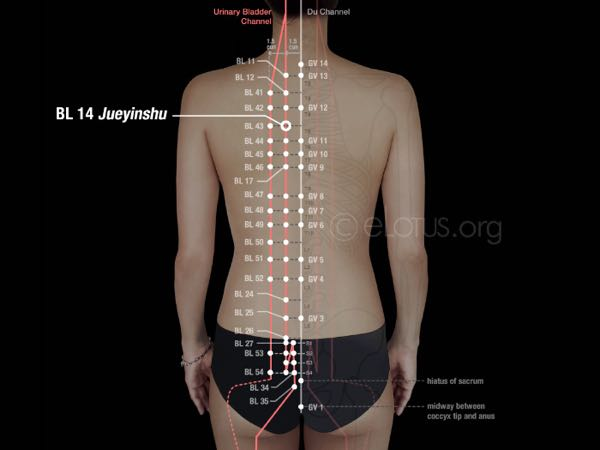
\includegraphics[width=\linewidth]{images/optimized/point_bl14.jpg}\caption{Hình minh họa huyệt BL 14.}\end{figure}
\subsection*{Chỉ định}Đau tim, hồi hộp, tức ngực ; Ho, nôn mửa;
\subsection*{Ứng dụng}Lan tỏa Khí Can và thả lỏng lồng ngực ; Điều hòa Tâm; Điều hòa và hạ khí;
\subsection*{Thủ thuật}Châm xiên 0,5-0,7 thốn. Không nên đặt vuông góc vì nó có thể gây tràn khí màng Phế.
\subsection*{Phân loại và ghi chú}Phân loại và ghi chú: Điểm Back Shu - Tâm Bào
\subsection{BL 15 - Tâm Du (Xinshu)}
\subsection*{Thông tin cơ bản}\begin{description}\item[Hán tự và phiên âm:] 心俞; xīn shū.\item[Ý nghĩa tên (theo tiếng Anh nguồn):] Du huyệt Tâm (dịch sát nghĩa; literal translation); tiếng Anh nguồn: Heart Shu, Heart Back Transporting Point.\end{description}
\subsection*{Vị trí}1,5 thốn về phía rìa dưới của quá trình gai của T5 [Thần Đạo e nM (GV 11) ].
\begin{figure}[H]\centering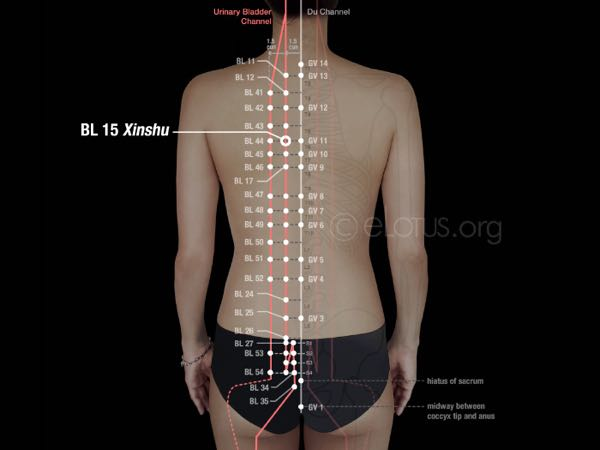
\includegraphics[width=\linewidth]{images/optimized/point_bl15.jpg}\caption{Hình minh họa huyệt BL 15.}\end{figure}
\subsection*{Chỉ định}Đau tim, hồi hộp, tức ngực ; Hưng cảm, động kinh, hoảng sợ, mất trí nhớ; Ho, khạc ra huyết; Khí thải về đêm, đổ mồ hôi đêm;
\subsection*{Ứng dụng}Săn chắc và nuôi dưỡng Tâm ; Điều hòa tâm khí, an thần; Nới lỏng lồng ngực và giải quyết tình trạng ứ huyết; Làm sạch lửa tim ;
\subsection*{Thủ thuật}Châm xiên 0,5-0,7 thốn. Không nên đặt vuông góc vì nó có thể gây tràn khí màng Phế.
\subsection*{Phân loại và ghi chú}Phân loại và ghi chú: Điểm quay lại Shu - Tâm
\subsection{BL 16 - Đốc Du (Dushu)}
\subsection*{Thông tin cơ bản}\begin{description}\item[Hán tự và phiên âm:] 督俞; dū shū.\item[Ý nghĩa tên (theo tiếng Anh nguồn):] Du huyệt Đốc (dịch sát nghĩa; literal translation); tiếng Anh nguồn: Governing Shu, Governor Shu, Du Channel Back Transporting Point.\end{description}
\subsection*{Vị trí}1,5 thốn phía bên tính đến bờ dưới của mỏm gai T6 [Linh Đài h Tu (GV 10) ].
\begin{figure}[H]\centering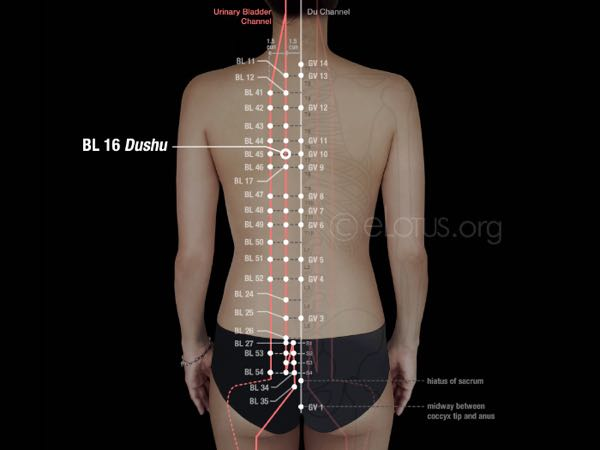
\includegraphics[width=\linewidth]{images/optimized/point_bl16.jpg}\caption{Hình minh họa huyệt BL 16.}\end{figure}
\subsection*{Chỉ định}Đau tim, đau vùng thượng vị ;
\subsection*{Ứng dụng}Điều hòa khí ở ngực và bụng ;
\subsection*{Thủ thuật}Châm xiên 0,5-0,7 thốn. Không nên đặt vuông góc vì nó có thể gây tràn khí màng Phế.
\subsection*{Phân loại và ghi chú}Điểm đặc biệt Ghi chú: Trở lại Shu Point - Kinh Du (Quản lý)
\subsection{BL 17 - Cách Du (Geshu)}
\subsection*{Thông tin cơ bản}\begin{description}\item[Hán tự và phiên âm:] 膈俞; gé shū.\item[Ý nghĩa tên (theo tiếng Anh nguồn):] Du huyệt Cách (dịch sát nghĩa; literal translation); tiếng Anh nguồn: Diaphragm Shu, Diaphragm Back Transporting Point.\end{description}
\subsection*{Vị trí}1,5 thốn bên tính đến bờ dưới của mỏm gai T7 [Chí Dương (GV 9) ].
\begin{figure}[H]\centering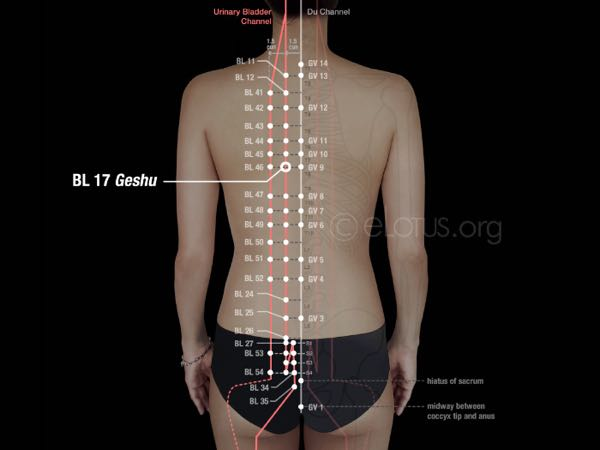
\includegraphics[width=\linewidth]{images/optimized/point_bl17.jpg}\caption{Hình minh họa huyệt BL 17.}\end{figure}
\subsection*{Chỉ định}Nôn mửa, nấc, ợ hơi, khạc ra huyết, khó nuốt ; Sốt chiều, đổ mồ hôi đêm, sởi; Hen suyễn, ho;
\subsection*{Ứng dụng}Bổ huyết, xua tan ứ ; Làm mát huyết, cầm huyết, nuôi dưỡng và điều hòa huyết; Điều hòa cơ hoành và hạ khí nổi loạn;
\subsection*{Thủ thuật}Châm xiên 0,5-0,7 thốn. Không nên đặt vuông góc vì nó có thể gây tràn khí màng Phế.
\subsection*{Phân loại và ghi chú}Phân loại và ghi chú: Điểm lưng Thục - Ge (Màng ngăn) 8 Huy điểm ảnh hưởng - Huyết
\subsection{BL 18 - Can Du (Ganshu)}
\subsection*{Thông tin cơ bản}\begin{description}\item[Hán tự và phiên âm:] 肝俞; gān shū.\item[Ý nghĩa tên (theo tiếng Anh nguồn):] Du huyệt Can (dịch sát nghĩa; literal translation); tiếng Anh nguồn: Liver Shu, Liver Back Transporting Point.\end{description}
\subsection*{Vị trí}1,5 thốn bên tính đến viền dưới của mỏm gai T9 [Cân Súc (GV 8) ].
\begin{figure}[H]\centering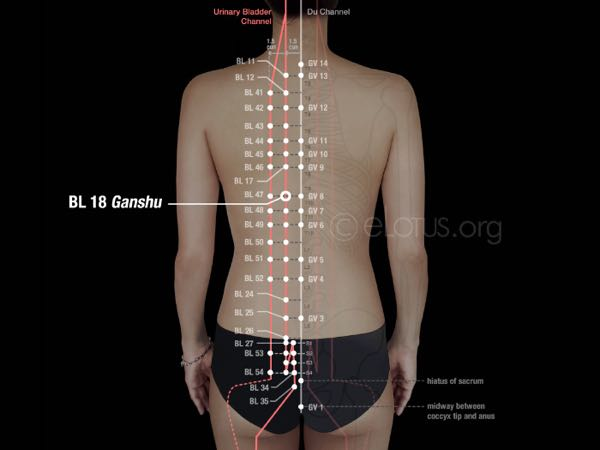
\includegraphics[width=\linewidth]{images/optimized/point_bl18.jpg}\caption{Hình minh họa huyệt BL 18.}\end{figure}
\subsection*{Chỉ định}Đau vùng hạ sườn, đau lưng ; Rối loạn tâm thần, động kinh; Vàng da, khạc ra huyết, chảy huyết cam; Đỏ mắt, mờ mắt, quáng gà;
\subsection*{Ứng dụng}Lan truyền khí Can ; Điều hòa và bổ Can, ích khí; Làm nguội lửa, thanh nhiệt; Lợi ích cho mắt và gân;
\subsection*{Thủ thuật}Châm xiên 0,5-0,7 thốn. Không nên đặt vuông góc vì nó có thể gây tràn khí màng Phế.
\subsection*{Phân loại và ghi chú}Phân loại và ghi chú: Điểm quay lại Shu - Can
\subsection{BL 19 - Đởm Du (Danshu)}
\subsection*{Thông tin cơ bản}\begin{description}\item[Hán tự và phiên âm:] 膽俞; dǎn shū.\item[Ý nghĩa tên (theo tiếng Anh nguồn):] Du huyệt Đởm (dịch sát nghĩa; literal translation); tiếng Anh nguồn: Gallbladder Shu, Gallbladder Back Transporting Point.\end{description}
\subsection*{Vị trí}1,5 thốn bên tính đến bờ dưới của mỏm gai T10 [Trung Khu (GV 7) ].
\begin{figure}[H]\centering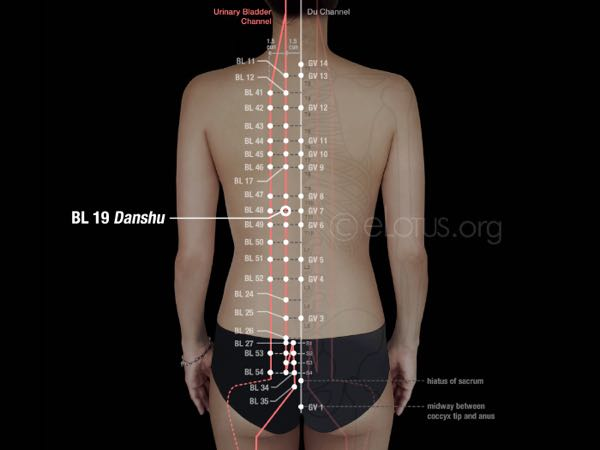
\includegraphics[width=\linewidth]{images/optimized/point_bl19.jpg}\caption{Hình minh họa huyệt BL 19.}\end{figure}
\subsection*{Chỉ định}Vàng da, miệng đắng ; Đau ở ngực và vùng hạ vị ; Lao Phế, sốt chiều ;
\subsection*{Ứng dụng}Thanh nhiệt ẩm từ Can và Đởm; Xóa các yếu tố gây bệnh từ thiếu dương; Tăng cường và điều hòa khí Đởm;
\subsection*{Thủ thuật}Châm xiên 0,5-0,8 thốn. Không nên đặt vuông góc vì nó có thể gây tràn khí màng Phế.
\subsection*{Phân loại và ghi chú}Phân loại và ghi chú: Điểm quay lại Shu - Đởm
\subsection{BL 20 - Tỳ Du (Pishu)}
\subsection*{Thông tin cơ bản}\begin{description}\item[Hán tự và phiên âm:] 脾俞; pí shū.\item[Ý nghĩa tên (theo tiếng Anh nguồn):] Du huyệt Tỳ (dịch sát nghĩa; literal translation); tiếng Anh nguồn: Spleen Shu, Spleen Back Transporting Point.\end{description}
\subsection*{Vị trí}1,5 thốn phía bên tính đến bờ dưới của mỏm gai T11 [Tích Trung (GV 6) ].
\begin{figure}[H]\centering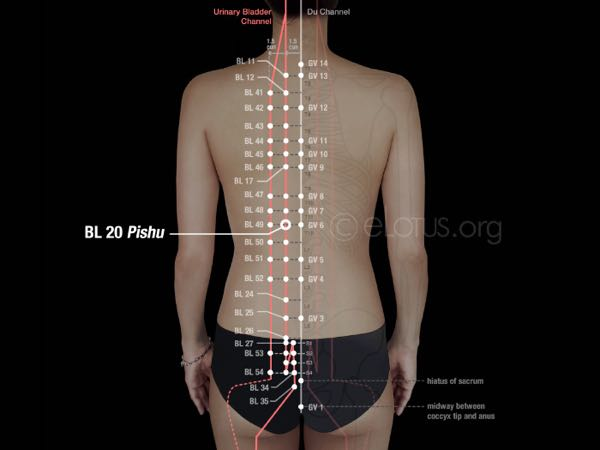
\includegraphics[width=\linewidth]{images/optimized/point_bl20.jpg}\caption{Hình minh họa huyệt BL 20.}\end{figure}
\subsection*{Chỉ định}Nôn mửa, tiêu chảy, lỵ, vàng da, phù nề, ; Phân có huyết, kinh nguyệt nhiều; Đau vùng thượng vị, chướng bụng, chán ăn, đau lưng;
\subsection*{Ứng dụng}Bổ tỳ khí dương, giải quyết ẩm thấp; Tăng Tỳ khí, cầm huyết; Điều hòa và điều hòa khí của trung jiao ;
\subsection*{Thủ thuật}Châm xiên 0,5-0,7 thốn. Không nên đặt vuông góc vì nó có thể gây tràn khí màng Phế.
\subsection*{Phân loại và ghi chú}Phân loại và ghi chú: Điểm Back Shu - Tỳ
\subsection{BL 21 - Vị Du (Weishu)}
\subsection*{Thông tin cơ bản}\begin{description}\item[Hán tự và phiên âm:] 胃俞; wèi shū.\item[Ý nghĩa tên (theo tiếng Anh nguồn):] Du huyệt Vị (dịch sát nghĩa; literal translation); tiếng Anh nguồn: Stomach Shu, Stomach Back Transporting Point.\end{description}
\subsection*{Vị trí}1,5 thốn về phía bên so với viền dưới của mỏm gai T12.
\begin{figure}[H]\centering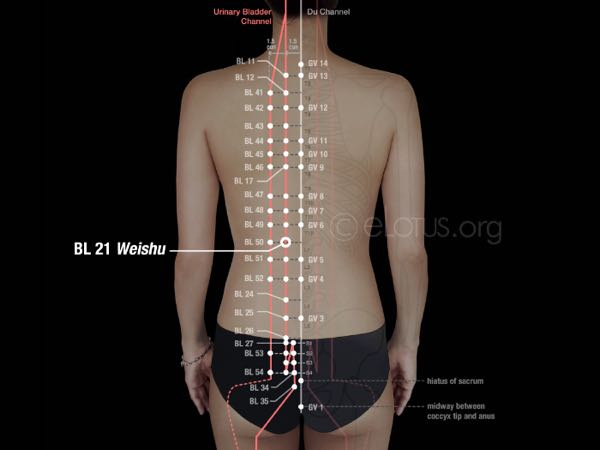
\includegraphics[width=\linewidth]{images/optimized/point_bl21.jpg}\caption{Hình minh họa huyệt BL 21.}\end{figure}
\subsection*{Chỉ định}Đau ở ngực, vùng hạ sườn và vùng thượng vị ; Chướng bụng, sôi bụng, trào ngược Vị, tiêu chảy; Buồn nôn, nôn, chán ăn;
\subsection*{Ứng dụng}Điều hòa và làm săn chắc Vị ; Hạ khí phản nghịch, giải ẩm ướt, tiêu trừ ứ đọng lương thực; Hài hòa jiao trung ;
\subsection*{Thủ thuật}Châm xiên 0,5-0,8 thốn. Không nên đặt vuông góc vì nó có thể gây tràn khí màng Phế.
\subsection*{Phân loại và ghi chú}Phân loại và ghi chú: Điểm quay lại Shu - Vị
\subsection{BL 22 - Tam Tiêu Du (Sanjiaoshu)}
\subsection*{Thông tin cơ bản}\begin{description}\item[Hán tự và phiên âm:] 三焦俞; sān jiāo shū.\item[Ý nghĩa tên (theo tiếng Anh nguồn):] Du huyệt Tam Tiêu (dịch sát nghĩa; literal translation); tiếng Anh nguồn: Triple Burner Shu, San Jiao Back Transporting Point.\end{description}
\subsection*{Vị trí}1,5 thốn phía bên tính đến bờ dưới của mỏm gai L1 [Huyền Khu (GV 5) ].
\begin{figure}[H]\centering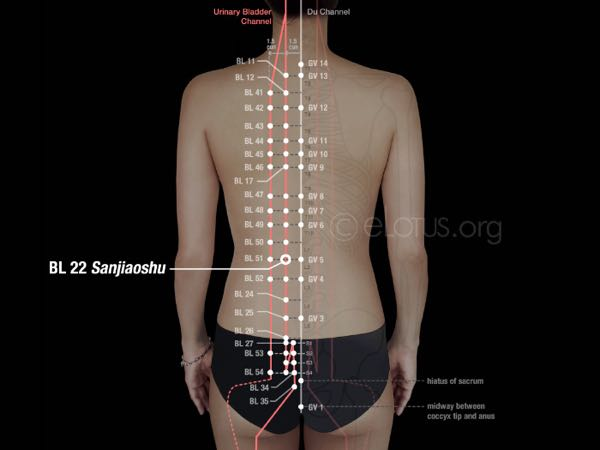
\includegraphics[width=\linewidth]{images/optimized/point_bl22.jpg}\caption{Hình minh họa huyệt BL 22.}\end{figure}
\subsection*{Chỉ định}Borborygmus, chướng bụng, khó tiêu, kiết lỵ ; Nôn mửa, tiêu chảy, phù nề; Đau và cứng vùng lưng dưới;
\subsection*{Ứng dụng}Di chuyển và điều hòa Tam Giao, điều hòa Tỳ và Vị ; Điều hòa đường dẫn nước, thúc đẩy tiểu tiện, giải quyết ẩm ướt;
\subsection*{Thủ thuật}Châm thẳng 0,5-1,0 thốn.
\subsection*{Phân loại và ghi chú}Phân loại và ghi chú: Điểm quay lại Shu - Tam Tiêu
\subsection{BL 23 - Thận Du (Shenshu)}
\subsection*{Thông tin cơ bản}\begin{description}\item[Hán tự và phiên âm:] 腎俞; shèn shū.\item[Ý nghĩa tên (theo tiếng Anh nguồn):] Du huyệt Thận (dịch sát nghĩa; literal translation); tiếng Anh nguồn: Kidney Shu, Kidney Back Transporting Point.\end{description}
\subsection*{Vị trí}1,5 thốn phía bên tính đến bờ dưới của mỏm gai L2 [Mệnh Môn (GV 4) ].
\begin{figure}[H]\centering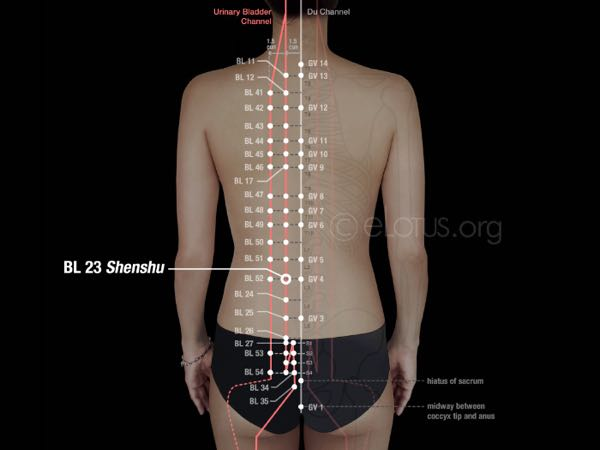
\includegraphics[width=\linewidth]{images/optimized/point_bl23.jpg}\caption{Hình minh họa huyệt BL 23.}\end{figure}
\subsection*{Chỉ định}Phát ban về đêm, bất lực, kinh nguyệt không đều, bạch cầu ; Hen suyễn, tiêu chảy, đái dầm, phù nề; Mờ mắt, chóng mặt, ù tai, điếc; Đau thắt lưng, yếu đầu gối;
\subsection*{Ứng dụng}Bổ Thận dương khí ; Nuôi Thận âm và tinh; Điều hòa đường dẫn nước, lợi tiểu; Lợi ích và làm ấm tử thống; Lợi ích cho tai và mắt; Tăng cường vùng thắt lưng;
\subsection*{Thủ thuật}Châm thẳng 1,0-1,2 thốn.
\subsection*{Phân loại và ghi chú}Phân loại và ghi chú: Điểm quay lại Shu - Thận
\subsection{BL 24 - Khí Hải Du (Qihaishu)}
\subsection*{Thông tin cơ bản}\begin{description}\item[Hán tự và phiên âm:] 氣海俞; qì hǎi shū.\item[Ý nghĩa tên (theo tiếng Anh nguồn):] Du huyệt biển Khí (dịch sát nghĩa; literal translation); tiếng Anh nguồn: Sea of Qi Shu, Sea of Qi Back Transporting Point.\end{description}
\subsection*{Vị trí}cách bờ dưới của mỏm gai L3 1,5 thốn.
\begin{figure}[H]\centering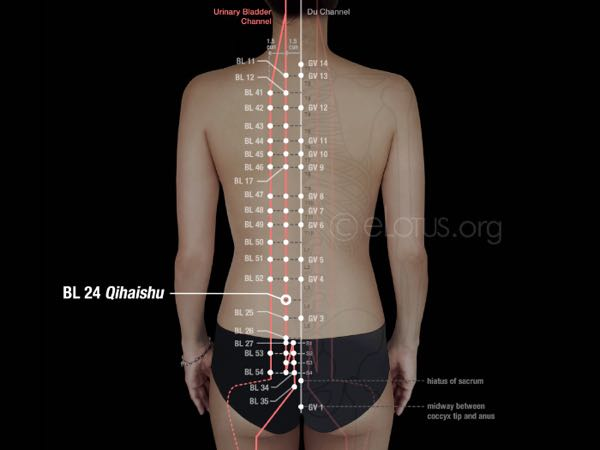
\includegraphics[width=\linewidth]{images/optimized/point_bl24.jpg}\caption{Hình minh họa huyệt BL 24.}\end{figure}
\subsection*{Chỉ định}Hen suyễn, đau lưng ; Kinh nguyệt không đều, đau bụng kinh;
\subsection*{Ứng dụng}Điều hòa khí huyết, tăng cường sức mạnh vùng thắt lưng và chân ; Điều chỉnh jiao dưới ;
\subsection*{Thủ thuật}Châm thẳng 0,8-1,2 thốn.
\subsection*{Phân loại và ghi chú}Điểm đặc biệt Ghi chú: Điểm Back Shu - Qihai (Biển Qi)
\subsection{BL 25 - Đại Trường Du (Dachangshu)}
\subsection*{Thông tin cơ bản}\begin{description}\item[Hán tự và phiên âm:] 大腸俞; dà cháng shū.\item[Ý nghĩa tên (theo tiếng Anh nguồn):] Du huyệt Đại Trường (dịch sát nghĩa; literal translation); tiếng Anh nguồn: Large Intestine Shu, Large Intestine Back Transporting Point.\end{description}
\subsection*{Vị trí}1,5 thốn về phía bờ dưới của mỏm gai L4 [ Yêu Dương Quan (GV 3) ].
\begin{figure}[H]\centering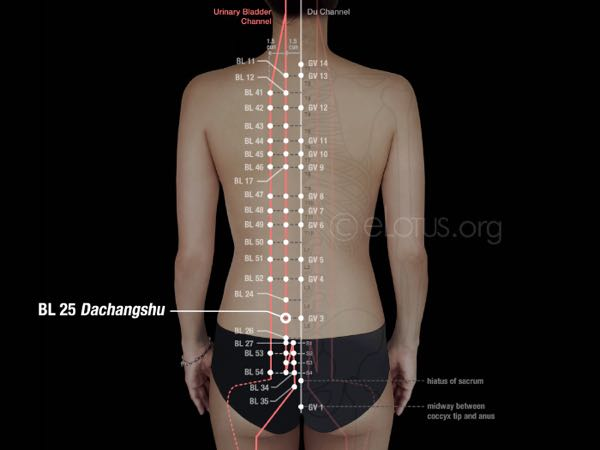
\includegraphics[width=\linewidth]{images/optimized/point_bl25.jpg}\caption{Hình minh họa huyệt BL 25.}\end{figure}
\subsection*{Chỉ định}Borborygmus, chướng bụng, tiêu chảy, táo bón ; Đau lưng, đau thần kinh tọa, teo cơ; Đau, tê, suy giảm vận động chi dưới;
\subsection*{Ứng dụng}Điều hòa đường ruột ; Loại bỏ tình trạng trì trệ, giảm đau; Tăng cường sức mạnh vùng thắt lưng và chân;
\subsection*{Thủ thuật}Châm thẳng 0,8-1,2 thốn.
\subsection*{Phân loại và ghi chú}Phân loại và ghi chú: Điểm quay lại Shu - LI
\subsection{BL 26 - Quan Nguyên Du (Guanyuanshu)}
\subsection*{Thông tin cơ bản}\begin{description}\item[Hán tự và phiên âm:] 關元俞; guān yuán shū.\item[Ý nghĩa tên (theo tiếng Anh nguồn):] Du huyệt Quan Nguyên (dịch sát nghĩa; literal translation); tiếng Anh nguồn: Origin Pass Shu, Origin Pass Back Transporting Point, Gate of Origin Shu.\end{description}
\subsection*{Vị trí}cách bờ dưới của mỏm gai L5 1,5 thốn.
\begin{figure}[H]\centering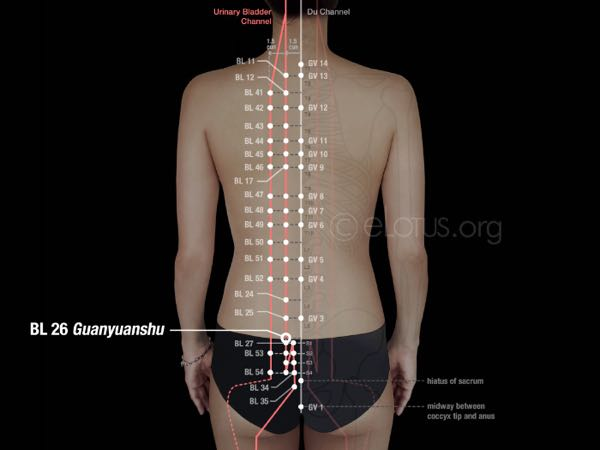
\includegraphics[width=\linewidth]{images/optimized/point_bl26.jpg}\caption{Hình minh họa huyệt BL 26.}\end{figure}
\subsection*{Chỉ định}Đau thắt lưng, đau thần kinh tọa ; Chướng bụng, tiêu chảy; Đái dầm, đi tiểu thường xuyên;
\subsection*{Ứng dụng}Tăng cường sức mạnh vùng thắt lưng ; Điều chỉnh jiao dưới ;
\subsection*{Thủ thuật}Châm thẳng 0,8-1,2 thốn.
\subsection*{Phân loại và ghi chú}Điểm đặc biệt Ghi chú: Điểm Back Shu - Guanyuan (Cổng nguồn)
\subsection{BL 27 - Tiểu Trường Du (Xiaochangshu)}
\subsection*{Thông tin cơ bản}\begin{description}\item[Hán tự và phiên âm:] 小腸俞; xiǎo cháng shū.\item[Ý nghĩa tên (theo tiếng Anh nguồn):] Du huyệt Tiểu Trường (dịch sát nghĩa; literal translation); tiếng Anh nguồn: Small Intestine Shu, Small Intestine Back Transporting Shu.\end{description}
\subsection*{Vị trí}cách đường giữa 1,5 thốn, ngang mức lỗ xương cùng sau thứ nhất.
\begin{figure}[H]\centering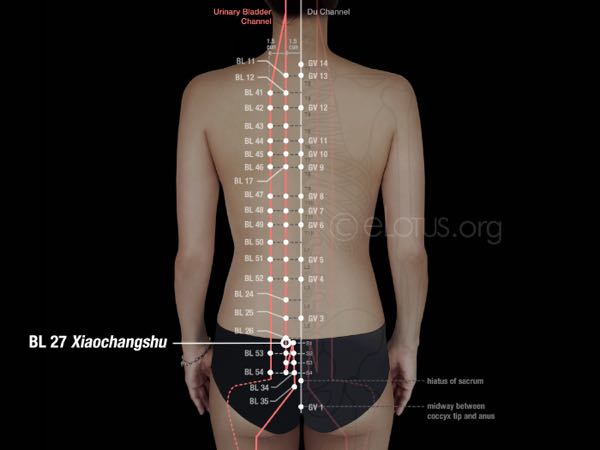
\includegraphics[width=\linewidth]{images/optimized/point_bl27.jpg}\caption{Hình minh họa huyệt BL 27.}\end{figure}
\subsection*{Chỉ định}Đau bụng dưới, chướng bụng ; Tiểu huyết, đái dầm, kiết lỵ; Xuất tinh về đêm, bệnh bạch cầu bệnh lý; Đau lưng dưới, đau thần kinh tọa;
\subsection*{Ứng dụng}Điều hòa ruột và Bàng Quang cũng như khí Tiểu Trường ; Tách chất tinh khiết khỏi chất đục; Thoát ẩm, thanh nhiệt;
\subsection*{Thủ thuật}Châm thẳng 0,8-1,2 thốn.
\subsection*{Phân loại và ghi chú}Phân loại và ghi chú: Điểm quay lại Shu - Tiểu Trường
\subsection{BL 28 - Bàng Quang Du (Pangguangshu)}
\subsection*{Thông tin cơ bản}\begin{description}\item[Hán tự và phiên âm:] 膀胱俞; páng guāng shū.\item[Ý nghĩa tên (theo tiếng Anh nguồn):] Du huyệt Bàng Quang (dịch sát nghĩa; literal translation); tiếng Anh nguồn: Bladder Shu, Bladder Back Transporting Point.\end{description}
\subsection*{Vị trí}cách đường giữa 1,5 thốn, ngang mức lỗ xương cùng sau thứ 2.
\begin{figure}[H]\centering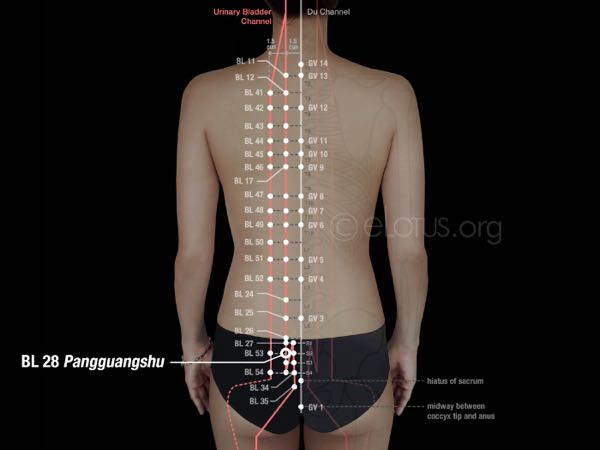
\includegraphics[width=\linewidth]{images/optimized/point_bl28.jpg}\caption{Hình minh họa huyệt BL 28.}\end{figure}
\subsection*{Chỉ định}Bí tiểu, đái dầm, đi tiểu thường xuyên ; Tiêu chảy, táo bón; Cứng, đau vùng thắt lưng;
\subsection*{Ứng dụng}Điều hòa Bàng Quang ; Xóa nhiệt ẩm từ jiao dưới; Xua tan sự trì trệ và giải quyết quần chúng; Có lợi cho vùng thắt lưng và chân;
\subsection*{Thủ thuật}Châm thẳng 0,8-1,2 thốn.
\subsection*{Phân loại và ghi chú}Phân loại và ghi chú: Điểm quay lại Shu - Bàng Quang
\subsection{BL 29 - Trung Lữ Du (Zhonglushu)}
\subsection*{Thông tin cơ bản}\begin{description}\item[Hán tự và phiên âm:] 中膂俞; zhōng lǚ shū.\item[Ý nghĩa tên (theo tiếng Anh nguồn):] Du huyệt giữa lưng (dịch sát nghĩa; literal translation); tiếng Anh nguồn: Central Backbone Shu, Mid-Spine Shu, Mid-Spine Back Transporting Point.\end{description}
\subsection*{Vị trí}cách đường giữa 1,5 thốn, ngang mức lỗ xương cùng sau thứ 3.
\begin{figure}[H]\centering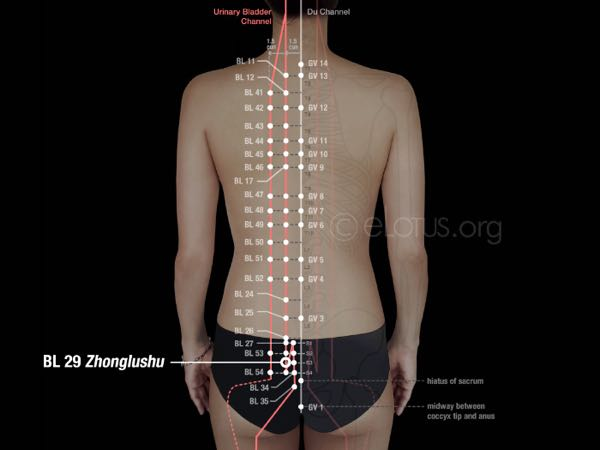
\includegraphics[width=\linewidth]{images/optimized/point_bl29.jpg}\caption{Hình minh họa huyệt BL 29.}\end{figure}
\subsection*{Chỉ định}Cứng khớp, đau lưng dưới ; kiết lỵ, thoát vị;
\subsection*{Ứng dụng}Có lợi cho vùng thắt lưng; Xua tan cảm lạnh, ngừng tiêu chảy;
\subsection*{Thủ thuật}Châm thẳng 0,8-1,2 thốn.
\subsection*{Phân loại và ghi chú}Phân loại và ghi chú: Điểm lưng Thục - Zhonglu (Cơ lưng trung tâm)
\subsection{BL 30 - Bạch Hoàn Du (Baihuanshu)}
\subsection*{Thông tin cơ bản}\begin{description}\item[Hán tự và phiên âm:] 白環俞; bái huán shū.\item[Ý nghĩa tên (theo tiếng Anh nguồn):] Du huyệt vòng trắng (dịch sát nghĩa; literal translation); tiếng Anh nguồn: White Ring Shu, White Ring Back Transporting Point.\end{description}
\subsection*{Vị trí}cách đường giữa 1,5 thốn, ngang mức lỗ xương cùng sau thứ 4.
\begin{figure}[H]\centering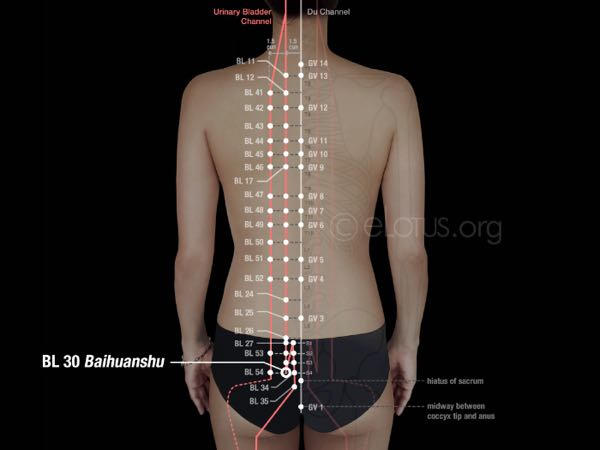
\includegraphics[width=\linewidth]{images/optimized/point_bl30.jpg}\caption{Hình minh họa huyệt BL 30.}\end{figure}
\subsection*{Chỉ định}Cảm giác lạnh và đau vùng thắt lưng, thoát vị ; Đái dầm, bệnh bạch cầu, kinh nguyệt không đều, xuất tinh; Khó tiểu, táo bón, mót rặn, sa trực tràng;
\subsection*{Ứng dụng}Có lợi cho vùng thắt lưng và chân ; Điều hòa kinh nguyệt và xuất tinh;
\subsection*{Thủ thuật}Châm thẳng 0,8-1,2 thốn.
\subsection*{Phân loại và ghi chú}Điểm đặc biệt Ghi chú: Điểm Back Shu - Baihuan (Vòng trắng)
\subsection{BL 31 - Thượng Liêu (Shangliao)}
\subsection*{Thông tin cơ bản}\begin{description}\item[Hán tự và phiên âm:] 上髎; shàng liáo.\item[Ý nghĩa tên (theo tiếng Anh nguồn):] Khe xương phía trên (dịch sát nghĩa; literal translation); tiếng Anh nguồn: Upper Bone Hole, Upper Crevice.\end{description}
\subsection*{Vị trí}Trên xương cùng, tại điểm giữa giữa gai chậu sau trên và đường giữa sau, ở lỗ xương cùng sau thứ nhất.
\begin{figure}[H]\centering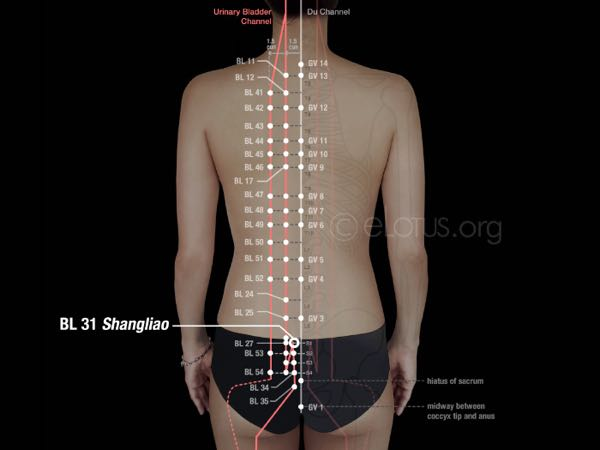
\includegraphics[width=\linewidth]{images/optimized/point_bl31.jpg}\caption{Hình minh họa huyệt BL 31.}\end{figure}
\subsection*{Chỉ định}Tiểu khó, sa tử thống, táo bón ; Kinh nguyệt không đều, bệnh bạch cầu, sa tử thống; Đau lưng dưới ;
\subsection*{Ứng dụng}Điều chỉnh jiao thấp hơn ; Điều hòa kinh nguyệt, trị bệnh bạch cầu; Có lợi cho vùng thắt lưng và chân;
\subsection*{Thủ thuật}Châm thẳng 0,8-1,2 thốn.
\subsection{BL 32 - Thứ Liêu (Ciliao)}
\subsection*{Thông tin cơ bản}\begin{description}\item[Hán tự và phiên âm:] 次髎; cì liáo.\item[Ý nghĩa tên (theo tiếng Anh nguồn):] Khe xương thứ hai (dịch sát nghĩa; literal translation); tiếng Anh nguồn: Second Bone Hole, Second Crevice.\end{description}
\subsection*{Vị trí}Trên xương cùng, trong và dưới cột sống chậu sau trên, ở lỗ xương cùng sau thứ 2.
\begin{figure}[H]\centering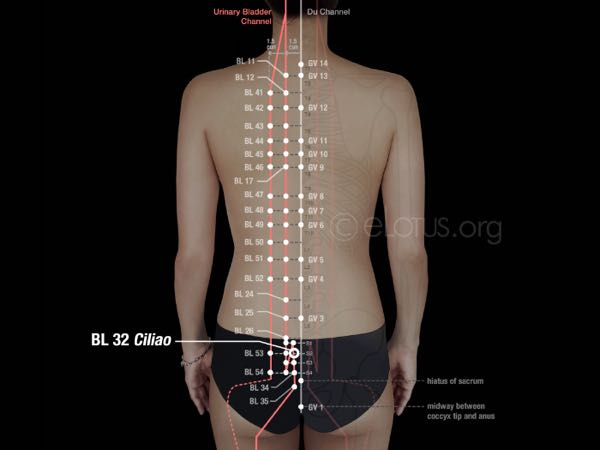
\includegraphics[width=\linewidth]{images/optimized/point_bl32.jpg}\caption{Hình minh họa huyệt BL 32.}\end{figure}
\subsection*{Chỉ định}Đái dầm, tiểu khó ; Kinh nguyệt không đều, khí hư, đau bụng kinh; Xuất tinh về đêm, bất lực; Đau thắt lưng, thoát vị; Teo cơ, đau, tê, suy giảm vận động chi dưới;
\subsection*{Ứng dụng}Điều chỉnh jiao thấp hơn ; Điều hòa kinh nguyệt, bổ Thận; Có lợi cho vùng thắt lưng và chân;
\subsection*{Thủ thuật}Châm thẳng 0,8-1,2 thốn.
\subsection{BL 33 - Trung Liêu (Zhongliao)}
\subsection*{Thông tin cơ bản}\begin{description}\item[Hán tự và phiên âm:] 中髎; zhōng liáo.\item[Ý nghĩa tên (theo tiếng Anh nguồn):] Khe xương giữa (dịch sát nghĩa; literal translation); tiếng Anh nguồn: Central Bone Hole, Middle Crevice.\end{description}
\subsection*{Vị trí}Trên xương cùng, trong và dưới Thứ Liêu (BL 32), ở lỗ xương cùng sau thứ 3.
\begin{figure}[H]\centering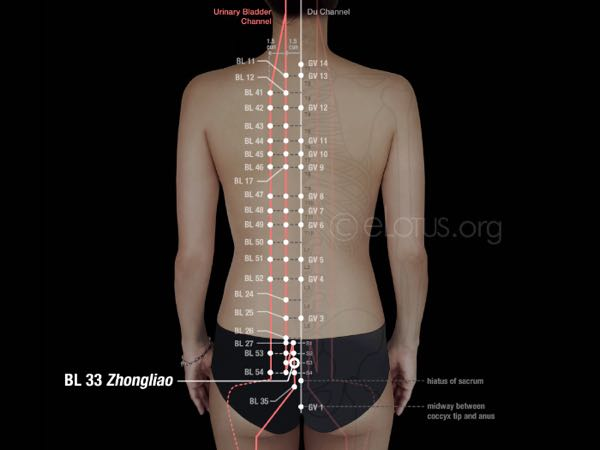
\includegraphics[width=\linewidth]{images/optimized/point_bl33.jpg}\caption{Hình minh họa huyệt BL 33.}\end{figure}
\subsection*{Chỉ định}Táo bón, tiêu chảy, khó tiểu ; Kinh nguyệt không đều, bệnh bạch cầu; Đau lưng dưới ;
\subsection*{Ứng dụng}Điều chỉnh jiao thấp hơn ; Điều hòa kinh nguyệt; Có lợi cho vùng thắt lưng và chân;
\subsection*{Thủ thuật}Châm thẳng 0,8-1,2 thốn.
\subsection{BL 34 - Hạ Liêu (Xialiao)}
\subsection*{Thông tin cơ bản}\begin{description}\item[Hán tự và phiên âm:] 下髎; xià liáo.\item[Ý nghĩa tên (theo tiếng Anh nguồn):] Khe xương phía dưới (dịch sát nghĩa; literal translation); tiếng Anh nguồn: Lower Bone Hole, Lower Crevice.\end{description}
\subsection*{Vị trí}Trên xương cùng, trong và dưới Trung Liêu h Tu (BL 33), ở lỗ xương cùng sau thứ 4.
\begin{figure}[H]\centering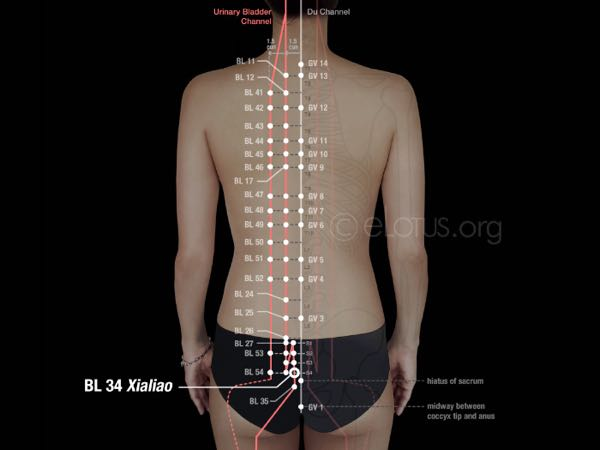
\includegraphics[width=\linewidth]{images/optimized/point_bl34.jpg}\caption{Hình minh họa huyệt BL 34.}\end{figure}
\subsection*{Chỉ định}Tiểu khó, táo bón, đau bụng dưới ; Bệnh bạch cầu bệnh lý; Đau lưng dưới ;
\subsection*{Ứng dụng}Điều chỉnh jiao thấp hơn ; Điều hòa kinh nguyệt; Có lợi cho vùng thắt lưng và chân;
\subsection*{Thủ thuật}Châm thẳng 0,8-1,2 thốn.
\subsection{BL 35 - Hội Dương (Huiyang)}
\subsection*{Thông tin cơ bản}\begin{description}\item[Hán tự và phiên âm:] 會陽; huì yáng.\item[Ý nghĩa tên (theo tiếng Anh nguồn):] Hội tụ Dương (dịch sát nghĩa; literal translation); tiếng Anh nguồn: Meeting of Yang.\end{description}
\subsection*{Vị trí}Trên xương cùng, cách đầu xương cụt 0,5 thốn.
\begin{figure}[H]\centering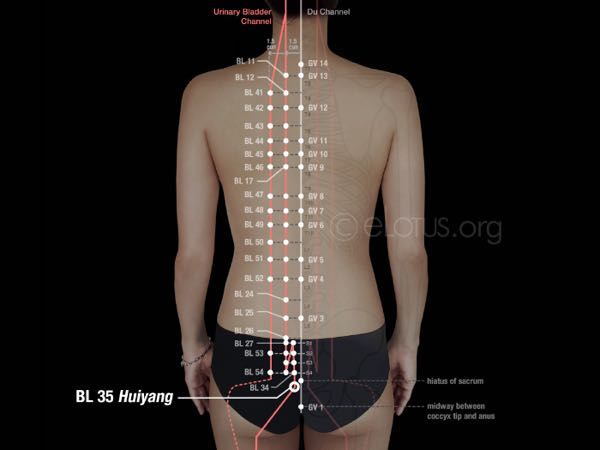
\includegraphics[width=\linewidth]{images/optimized/point_bl35.jpg}\caption{Hình minh họa huyệt BL 35.}\end{figure}
\subsection*{Chỉ định}Lỵ, tiêu chảy, đại tiện ra huyết, trĩ ; Bất lực, bệnh bạch cầu;
\subsection*{Ứng dụng}Loại bỏ nhiệt ẩm và điều chỉnh jiao phía dưới ; Lợi ích xương cụt ;
\subsection*{Thủ thuật}Châm thẳng 0,5-1,0 thốn.
\subsection{BL 36 - Thừa Phù (Chengfu)}
\subsection*{Thông tin cơ bản}\begin{description}\item[Hán tự và phiên âm:] 承扶; chéng fú.\item[Ý nghĩa tên (theo tiếng Anh nguồn):] Nâng đỡ (dịch sát nghĩa; literal translation); tiếng Anh nguồn: Support, Receiving Support, Hold and Support.\end{description}
\subsection*{Vị trí}Ở phía sau đùi, ngay dưới mông, ở điểm giữa của nếp gấp ngang cơ mông.
\begin{figure}[H]\centering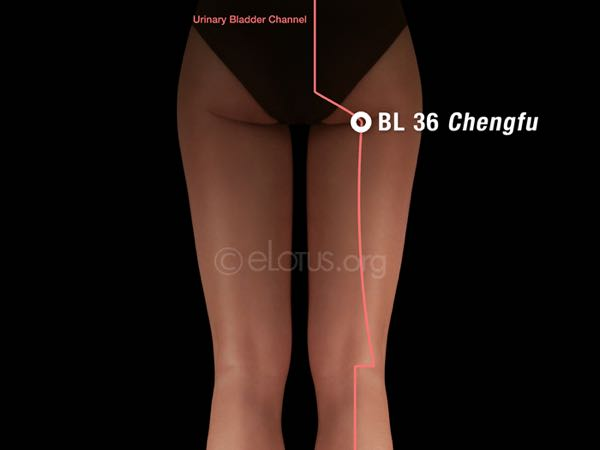
\includegraphics[width=\linewidth]{images/optimized/point_bl36.jpg}\caption{Hình minh họa huyệt BL 36.}\end{figure}
\subsection*{Chỉ định}Đau ở vùng lưng dưới và vùng mông ; Đau, tê, teo cơ, suy giảm vận động chi dưới; Táo bón, trĩ;
\subsection*{Ứng dụng}Kích hoạt kinh, thư giãn gân cốt, giảm đau ; Điều chỉnh jiao dưới ;
\subsection*{Thủ thuật}Châm thẳng 1,0-1,5 thốn.
\subsection{BL 37 - Ân Môn (Yinmen)}
\subsection*{Thông tin cơ bản}\begin{description}\item[Hán tự và phiên âm:] 殷門; yīn mén.\item[Ý nghĩa tên (theo tiếng Anh nguồn):] Cửa sung túc (dịch sát nghĩa; literal translation); tiếng Anh nguồn: Gate of Abundance, Door of Abundance.\end{description}
\subsection*{Vị trí}6 thốn dưới Thừa Phù (BL 36) trên đường nối Thừa Phù (BL 36) và Uỷ Trung (BL 40) , ở chỗ lõm giữa các cơ gân kheo.
\begin{figure}[H]\centering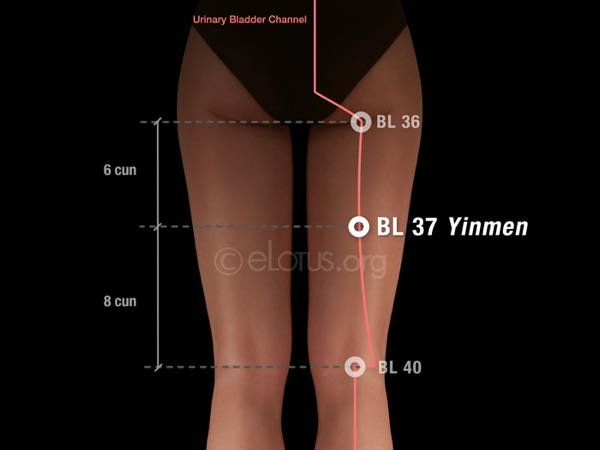
\includegraphics[width=\linewidth]{images/optimized/point_bl37.jpg}\caption{Hình minh họa huyệt BL 37.}\end{figure}
\subsection*{Chỉ định}Đau ở lưng dưới và đùi ; Teo cơ, đau, tê, suy giảm vận động chi dưới; liệt nửa người;
\subsection*{Ứng dụng}Kích hoạt kinh và giảm bớt cơn đau; Có lợi cho cột sống thắt lưng;
\subsection*{Thủ thuật}Châm thẳng 1,0-2,0 thốn.
\subsection{BL 38 - Phù Khích (Fuxi)}
\subsection*{Thông tin cơ bản}\begin{description}\item[Hán tự và phiên âm:] 浮郄; fú xī.\item[Ý nghĩa tên (theo tiếng Anh nguồn):] Khe nông (dịch sát nghĩa; literal translation); tiếng Anh nguồn: Superficial Cleft, Floating Cleft.\end{description}
\subsection*{Vị trí}Với đầu gối hơi gập, điểm này cao hơn Vị Dương (BL 39) 1 thốn trên đường viền trong của gân cơ bắp tay đùi.
\begin{figure}[H]\centering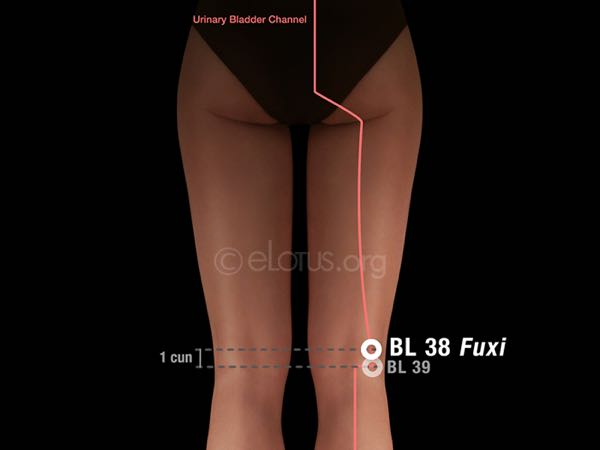
\includegraphics[width=\linewidth]{images/optimized/point_bl38.jpg}\caption{Hình minh họa huyệt BL 38.}\end{figure}
\subsection*{Chỉ định}Tê vùng mông và xương đùi ; Co rút các gân ở hố khoeo;
\subsection*{Ứng dụng}Thư giãn gân cốt và giảm đau ; Thanh nhiệt, làm dịu cơn chuột rút;
\subsection*{Thủ thuật}Châm thẳng 0,5-1,0 thốn.
\subsection{BL 39 - Uỷ Dương (Weiyang)}
\subsection*{Thông tin cơ bản}\begin{description}\item[Hán tự và phiên âm:] 委陽; wěi yáng.\item[Ý nghĩa tên (theo tiếng Anh nguồn):] Dương ở giữa chỗ khoeo (dịch sát nghĩa; literal translation); tiếng Anh nguồn: Bend Yang, Supporting the Yang, Outside the Crook.\end{description}
\subsection*{Vị trí}Với đầu gối hơi gập, điểm này nằm trên nếp gấp khoeo, bên cạnh Uỷ Trung (BL 40), trên đường viền trong của gân cơ bắp tay đùi.
\begin{figure}[H]\centering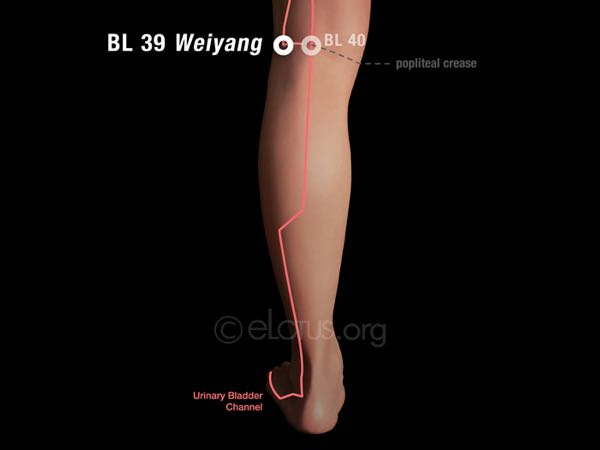
\includegraphics[width=\linewidth]{images/optimized/point_bl39.jpg}\caption{Hình minh họa huyệt BL 39.}\end{figure}
\subsection*{Chỉ định}Chướng bụng, đầy bụng, phù nề, tiểu khó ; Cứng khớp, đau lưng dưới, chuột rút ở chân và bàn chân;
\subsection*{Ứng dụng}Điều hòa Tam Giao và điều hòa tiểu tiện ; Kích hoạt kinh, giảm đau;
\subsection*{Thủ thuật}Châm thẳng 0,5-1,0 thốn.
\subsection*{Phân loại và ghi chú}Điểm đặc biệt Ghi chú: Điểm biển Hạ He - Tam Tiêu
\subsection{BL 42 - Phách Hộ (Pohu)}
\subsection*{Thông tin cơ bản}\begin{description}\item[Hán tự và phiên âm:] 魄戶; pò hù.\item[Ý nghĩa tên (theo tiếng Anh nguồn):] Cửa Phách (dịch sát nghĩa; literal translation); tiếng Anh nguồn: Po Door, Door of the Corporeal Soul.\end{description}
\subsection*{Vị trí}3 thốn về phía ngoài so với đường giữa, ngang với bờ dưới của mỏm gai T3 và Phế Du (BL 13), trên bờ cột sống của xương bả vai.
\begin{figure}[H]\centering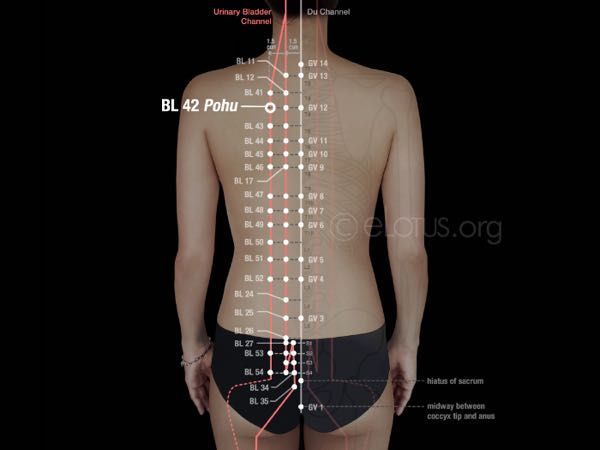
\includegraphics[width=\linewidth]{images/optimized/point_bl42.jpg}\caption{Hình minh họa huyệt BL 42.}\end{figure}
\subsection*{Chỉ định}Lao Phế, ho ra huyết, làm dịu khó thở, giảm ho, hen suyễn ; Cổ cứng, đau ở vai và lưng;
\subsection*{Ứng dụng}Bổ Phế, điều hòa và chế ngự Khí Phế nổi loạn ; Kích hoạt kinh, giảm đau;
\subsection*{Thủ thuật}Châm xiên 0,3-0,5 thốn. Không nên đặt vuông góc vì nó có thể gây tràn khí màng Phế.
\subsection{BL 43 - Cao Hoang Du (Gaohuangshu)}
\subsection*{Thông tin cơ bản}\begin{description}\item[Hán tự và phiên âm:] 膏肓俞; gāo huāng shū.\item[Ý nghĩa tên (theo tiếng Anh nguồn):] Du huyệt vùng Cao Hoang (dịch sát nghĩa; literal translation); tiếng Anh nguồn: Vital Region Shu, Vital's Back Transporting Point.\end{description}
\subsection*{Vị trí}3 thốn về phía ngoài so với đường giữa, ngang với bờ dưới của mỏm gai T4 và Quyết Âm Du (BL 14), trên bờ cột sống của xương bả vai.
\begin{figure}[H]\centering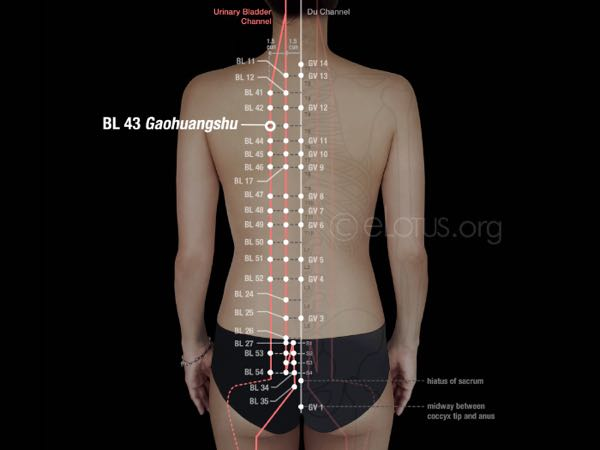
\includegraphics[width=\linewidth]{images/optimized/point_bl43.jpg}\caption{Hình minh họa huyệt BL 43.}\end{figure}
\subsection*{Chỉ định}Lao Phế, ho, hen suyễn, khạc ra huyết ; Đổ mồ hôi ban đêm, xuất tinh về đêm; Trí nhớ kém;
\subsection*{Ứng dụng}Tăng cường và nuôi dưỡng Phế, tim, Thận, Tỳ, Vị; Nuôi âm, thanh nhiệt; An thần; Hỗ trợ nhân dân tệ (nguồn) qi ; Giải quyết đờm;
\subsection*{Thủ thuật}Châm xiên 0,3-0,5 thốn. Không nên đặt vuông góc vì nó có thể gây tràn khí màng Phế. Điểm đặc biệt của
\subsection*{Phân loại và ghi chú}Ghi chú: Điểm Back Shu - Gaohuang (Vùng quan trọng)
\subsection{BL 44 - Thần Đường (Shentang)}
\subsection*{Thông tin cơ bản}\begin{description}\item[Hán tự và phiên âm:] 神堂; shén táng.\item[Ý nghĩa tên (theo tiếng Anh nguồn):] Sảnh thần trí (dịch sát nghĩa; literal translation); tiếng Anh nguồn: Spirit Hall, Hall of the Spirit.\end{description}
\subsection*{Vị trí}3 thốn về phía ngoài so với đường giữa, ngang với bờ dưới của mỏm gai T5 và Tâm Du (BL 15), trên bờ cột sống của xương bả vai.
\begin{figure}[H]\centering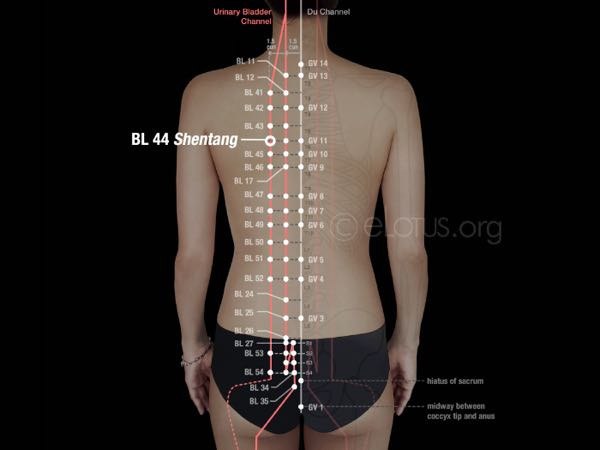
\includegraphics[width=\linewidth]{images/optimized/point_bl44.jpg}\caption{Hình minh họa huyệt BL 44.}\end{figure}
\subsection*{Chỉ định}Hen suyễn, tức ngực, ho ; Đau tim, đánh trống ngực; Cứng và đau lưng;
\subsection*{Ứng dụng}Nới lỏng lồng ngực, điều hòa khí ; Kích hoạt kinh, giảm đau;
\subsection*{Thủ thuật}Châm xiên 0,3-0,5 thốn. Không nên đặt vuông góc vì nó có thể gây tràn khí màng Phế.
\subsection{BL 45 - Y Hy (Yixi)}
\subsection*{Thông tin cơ bản}\begin{description}\item[Hán tự và phiên âm:] 譩譆; yì xǐ.\item[Ý nghĩa tên (theo tiếng Anh nguồn):] Điều bất ngờ (dịch sát nghĩa; literal translation); tiếng Anh nguồn: Surprise.\end{description}
\subsection*{Vị trí}3 thốn về phía ngoài so với đường giữa, ngang với bờ dưới của mỏm gai T6 và Đốc Du h Tu (BL 16), trên bờ cột sống của xương bả vai.
\begin{figure}[H]\centering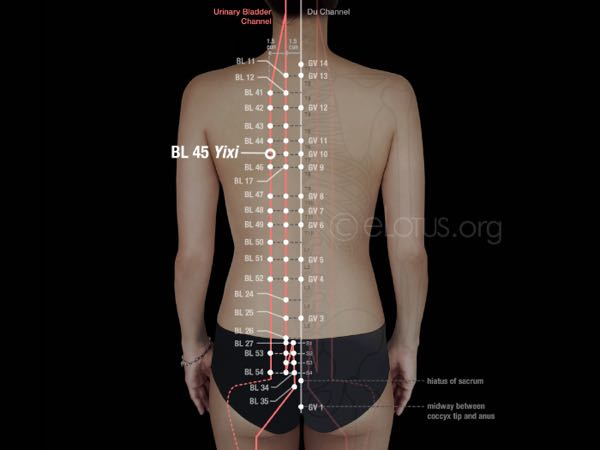
\includegraphics[width=\linewidth]{images/optimized/point_bl45.jpg}\caption{Hình minh họa huyệt BL 45.}\end{figure}
\subsection*{Chỉ định}Ho, hen suyễn ; Đau vai và lưng;
\subsection*{Ứng dụng}Đẩy gió, thanh nhiệt, giáng khí Phế; Tiếp thêm sinh lực khí huyết, giảm đau;
\subsection*{Thủ thuật}Châm xiên xuống 0,3-0,5 thốn. Không nên đặt vuông góc vì nó có thể gây tràn khí màng Phế.
\subsection{BL 46 - Cách Quan (Geguan)}
\subsection*{Thông tin cơ bản}\begin{description}\item[Hán tự và phiên âm:] 膈關; gé guān.\item[Ý nghĩa tên (theo tiếng Anh nguồn):] Cửa Cách (dịch sát nghĩa; literal translation); tiếng Anh nguồn: Diaphragm Pass, Diaphragm Hinge, Diaphragm Gate.\end{description}
\subsection*{Vị trí}3 thốn về phía ngoài so với đường giữa, ngang với bờ dưới của mỏm gai T7 và Cách Du (BL 17), và ngang mức góc dưới của xương bả vai.
\begin{figure}[H]\centering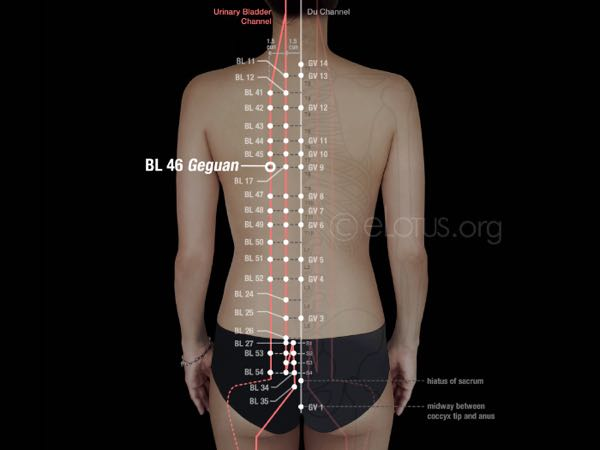
\includegraphics[width=\linewidth]{images/optimized/point_bl46.jpg}\caption{Hình minh họa huyệt BL 46.}\end{figure}
\subsection*{Chỉ định}Khó nuốt, nấc, nôn, ợ hơi; Đau và cứng lưng;
\subsection*{Ứng dụng}Điều hòa cơ hoành, có lợi cho trung jiao, hạ khí phản loạn; Kích hoạt kinh, giảm đau;
\subsection*{Thủ thuật}Châm xiên 0,3-0,5 thốn. Không nên đặt vuông góc vì nó có thể gây tràn khí màng Phế.
\subsection{BL 47 - Hồn Môn (Hunmen)}
\subsection*{Thông tin cơ bản}\begin{description}\item[Hán tự và phiên âm:] 魂門; hún mén.\item[Ý nghĩa tên (theo tiếng Anh nguồn):] Cửa Hồn (dịch sát nghĩa; literal translation); tiếng Anh nguồn: Hun Gate, Gate of the Ethereal Soul, Door of the Ethereal Soul.\end{description}
\subsection*{Vị trí}3 thốn về phía ngoài so với đường giữa, ngang với bờ dưới của mỏm gai T9 và Canshu (BL 18) .
\begin{figure}[H]\centering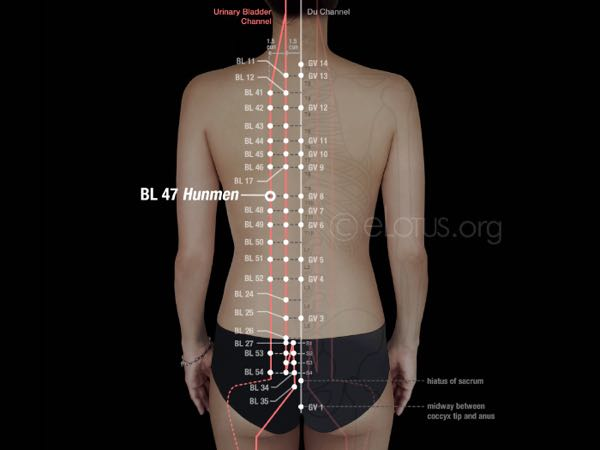
\includegraphics[width=\linewidth]{images/optimized/point_bl47.jpg}\caption{Hình minh họa huyệt BL 47.}\end{figure}
\subsection*{Chỉ định}Đau ở ngực và vùng hạ sườn, đau lưng ; Nôn mửa, tiêu chảy;
\subsection*{Ứng dụng}Phát tán khí Can, thư giãn gân cốt; Hài hòa jiao trung ;
\subsection*{Thủ thuật}Châm xiên 0,3-0,5 thốn. Không nên đặt vuông góc vì nó có thể gây tràn khí màng Phế.
\subsection{BL 48 - Dương Cương (Yanggang)}
\subsection*{Thông tin cơ bản}\begin{description}\item[Hán tự và phiên âm:] 陽綱; yáng gāng.\item[Ý nghĩa tên (theo tiếng Anh nguồn):] Mối nối chủ yếu của Dương (dịch sát nghĩa; literal translation); tiếng Anh nguồn: Yang Headrope, Yang's Key Link, Parameter of Yang.\end{description}
\subsection*{Vị trí}3 thốn về phía ngoài so với đường giữa, ngang với bờ dưới của mỏm gai T10 và Đởm Du (BL 19) .
\begin{figure}[H]\centering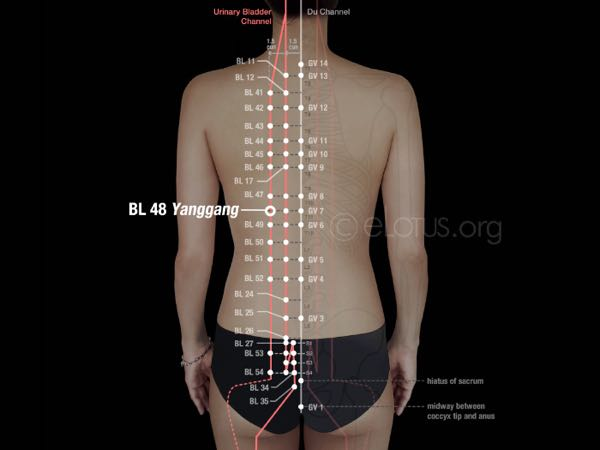
\includegraphics[width=\linewidth]{images/optimized/point_bl48.jpg}\caption{Hình minh họa huyệt BL 48.}\end{figure}
\subsection*{Chỉ định}Đau vùng hạ sườn, vàng da ; Borborygmus, đau bụng, tiêu chảy, ;
\subsection*{Ứng dụng}Điều hòa Đởm và thanh nhiệt ẩm; Hài hòa jiao trung ;
\subsection*{Thủ thuật}Châm xiên 0,3-0,5 thốn. Không nên đặt vuông góc vì nó có thể gây tràn khí màng Phế.
\subsection{BL 49 - Ý Xá (Yishe)}
\subsection*{Thông tin cơ bản}\begin{description}\item[Hán tự và phiên âm:] 意舍; yì shě.\item[Ý nghĩa tên (theo tiếng Anh nguồn):] Nhà của ý nghĩ (dịch sát nghĩa; literal translation); tiếng Anh nguồn: Reflection Abode, Abode of Thought, Thought Shelter.\end{description}
\subsection*{Vị trí}3 thốn về phía ngoài so với đường giữa, ngang với bờ dưới của mỏm gai T11 và Tỳ Du (BL 20) .
\begin{figure}[H]\centering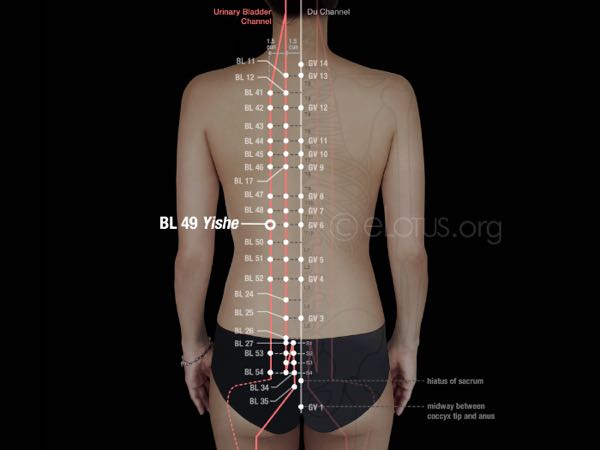
\includegraphics[width=\linewidth]{images/optimized/point_bl49.jpg}\caption{Hình minh họa huyệt BL 49.}\end{figure}
\subsection*{Chỉ định}Chướng bụng, borborygmus ; Nôn mửa, tiêu chảy; Khó nuốt;
\subsection*{Ứng dụng}Loại bỏ nhiệt ẩm; Điều hòa Tỳ và Vị;
\subsection*{Thủ thuật}Châm xiên 0,3-0,5 inch. Không nên đặt vuông góc vì nó có thể gây tràn khí màng Phế.
\subsection{BL 50 - Vị Thương (Weicang)}
\subsection*{Thông tin cơ bản}\begin{description}\item[Hán tự và phiên âm:] 胃倉; wèi cāng.\item[Ý nghĩa tên (theo tiếng Anh nguồn):] Kho chứa của Vị (dịch sát nghĩa; literal translation); tiếng Anh nguồn: Stomach Granary, Storehouse of Stomach.\end{description}
\subsection*{Vị trí}3 thốn về phía ngoài so với đường giữa, ngang với bờ dưới của mỏm gai T12 và Vị Du e nM (BL 21) .
\begin{figure}[H]\centering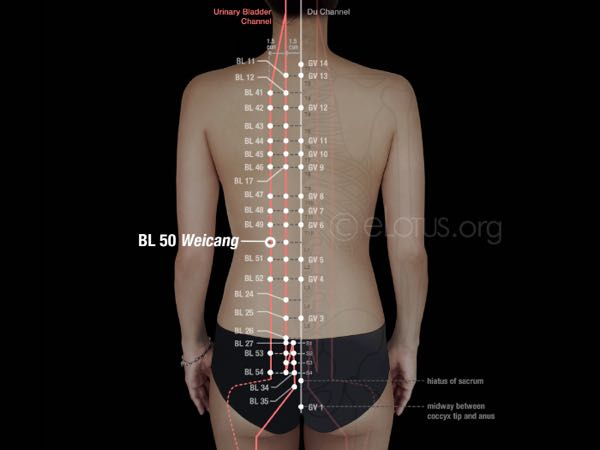
\includegraphics[width=\linewidth]{images/optimized/point_bl50.jpg}\caption{Hình minh họa huyệt BL 50.}\end{figure}
\subsection*{Chỉ định}Bụng chướng ; Đau vùng thượng vị và lưng; Chứng khó tiêu ở trẻ sơ sinh;
\subsection*{Ứng dụng}Hài hòa âm trung ;
\subsection*{Thủ thuật}Châm xiên 0,3-0,5 thốn. Không nên đặt vuông góc vì nó có thể gây tràn khí màng Phế.
\subsection{BL 51 - Hoang Môn (Huangmen)}
\subsection*{Thông tin cơ bản}\begin{description}\item[Hán tự và phiên âm:] 肓門; huāng mén.\item[Ý nghĩa tên (theo tiếng Anh nguồn):] Cửa Hoang (dịch sát nghĩa; literal translation); tiếng Anh nguồn: Huang Gate, Vitals Gate, Vitals Door.\end{description}
\subsection*{Vị trí}3 thốn về phía ngoài so với đường giữa, ngang với bờ dưới của mỏm gai L1 và Tam Tiêu Du (BL 22) .
\begin{figure}[H]\centering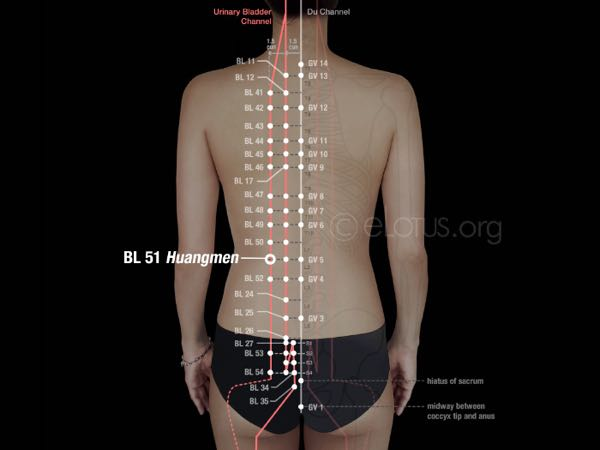
\includegraphics[width=\linewidth]{images/optimized/point_bl51.jpg}\caption{Hình minh họa huyệt BL 51.}\end{figure}
\subsection*{Chỉ định}Đau bụng, có khối u ở bụng ; Táo bón ;
\subsection*{Ứng dụng}Xua tan sự trì trệ;
\subsection*{Thủ thuật}Châm xiên 0,3-0,5 thốn.
\subsection{BL 52 - Chí Thất (Zhishi)}
\subsection*{Thông tin cơ bản}\begin{description}\item[Hán tự và phiên âm:] 志室; zhì shì.\item[Ý nghĩa tên (theo tiếng Anh nguồn):] Phòng chứa ý chí (dịch sát nghĩa; literal translation); tiếng Anh nguồn: Will Chamber, Residence of Will, Will Power Room.\end{description}
\subsection*{Vị trí}3 thốn về phía ngoài so với đường giữa, ngang với bờ dưới của mỏm gai L2 và Thận Du (BL 23) .
\begin{figure}[H]\centering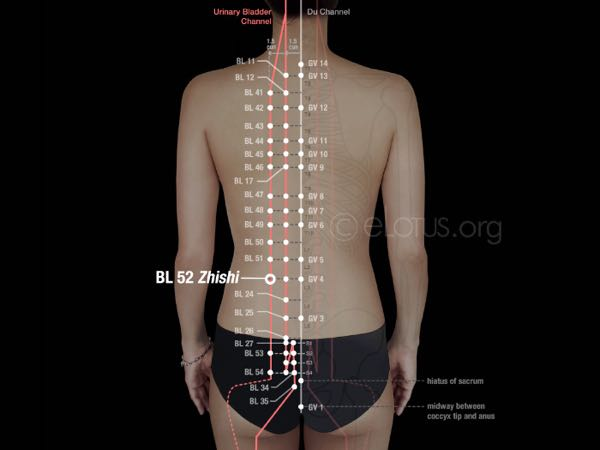
\includegraphics[width=\linewidth]{images/optimized/point_bl52.jpg}\caption{Hình minh họa huyệt BL 52.}\end{figure}
\subsection*{Chỉ định}Xuất tinh về đêm, bất lực, kinh nguyệt không đều ; Đái dầm, đi tiểu nhiều, khó tiểu, phù nề; Đau lưng và đầu gối;
\subsection*{Ứng dụng}Bổ Thận và bổ ích tinh chất ; Điều hòa đi tiểu; Tăng cường vùng thắt lưng;
\subsection*{Thủ thuật}Châm thẳng 0,5-1,0 thốn.
\subsection{BL 53 - Bào Hoang (Baohuang)}
\subsection*{Thông tin cơ bản}\begin{description}\item[Hán tự và phiên âm:] 胞肓; bāo huāng.\item[Ý nghĩa tên (theo tiếng Anh nguồn):] Hoang vùng Bào (dịch sát nghĩa; literal translation); tiếng Anh nguồn: Bladder Huang, Bladder Vitals.\end{description}
\subsection*{Vị trí}cách đường giữa 3 thốn, ngang mức lỗ xương cùng sau thứ 2.
\begin{figure}[H]\centering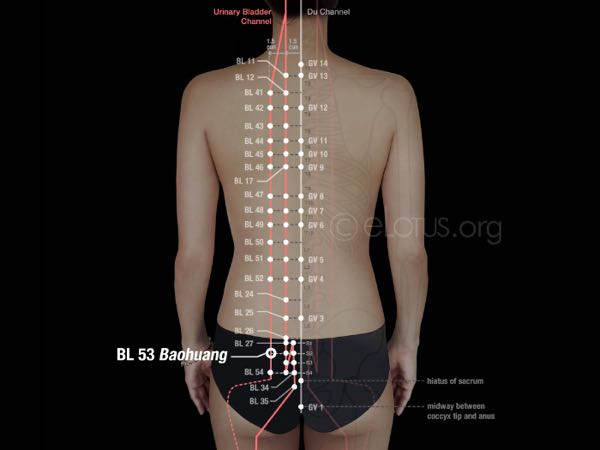
\includegraphics[width=\linewidth]{images/optimized/point_bl53.jpg}\caption{Hình minh họa huyệt BL 53.}\end{figure}
\subsection*{Chỉ định}Đau lưng dưới ; Borborygmus, chướng bụng, vô niệu ;
\subsection*{Ứng dụng}Có lợi cho vùng thắt lưng, kích hoạt kinh, giảm đau; Điều hòa hạ tiêu, ích lợi tiểu tiện;
\subsection*{Thủ thuật}Châm thẳng 0,8-1,2 thốn.
\subsection{BL 54 - Trật Biên (Zhibian)}
\subsection*{Thông tin cơ bản}\begin{description}\item[Hán tự và phiên âm:] 秩邊; zhì biān.\item[Ý nghĩa tên (theo tiếng Anh nguồn):] Ranh giới tuần tự (dịch sát nghĩa; literal translation); tiếng Anh nguồn: Sequential Limit, Order's Limit, Lowermost Edge.\end{description}
\subsection*{Vị trí}cách đường giữa 3 thốn, ngang mức lỗ xương cùng sau thứ 4.
\begin{figure}[H]\centering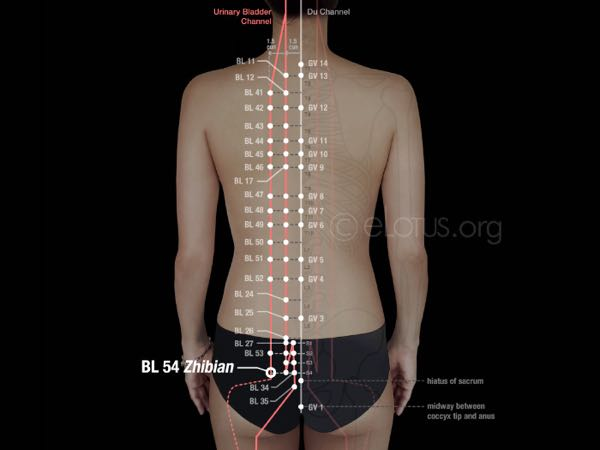
\includegraphics[width=\linewidth]{images/optimized/point_bl54.jpg}\caption{Hình minh họa huyệt BL 54.}\end{figure}
\subsection*{Chỉ định}Đau vùng thắt lưng cùng, teo cơ, suy giảm vận động chi dưới ; Tiểu khó, táo bón; Sưng quanh cơ quan sinh dục ngoài, trĩ;
\subsection*{Ứng dụng}Có lợi cho vùng thắt lưng, kích hoạt kinh và giảm đau; Điều hòa đi tiểu;
\subsection*{Thủ thuật}Châm thẳng 1,5-2,0 thốn.
\subsection{BL 55 - Hợp Dương (Heyang)}
\subsection*{Thông tin cơ bản}\begin{description}\item[Hán tự và phiên âm:] 合陽; hé yáng.\item[Ý nghĩa tên (theo tiếng Anh nguồn):] Hội tụ Dương (dịch sát nghĩa; literal translation); tiếng Anh nguồn: Yang Union, Confluence of Yang.\end{description}
\subsection*{Vị trí}2 thốn ngay dưới Uỷ Trung (BL 40) , giữa đầu trong và ngoài của cơ bụng chân, trên đường nối Uỷ Trung (BL 40) và Thừa Sơn (BL 57) .
\begin{figure}[H]\centering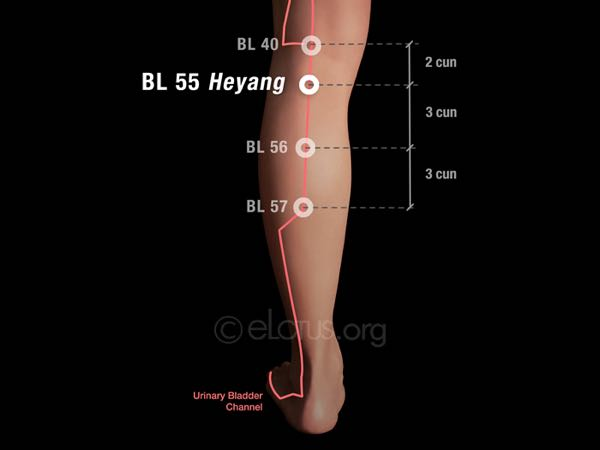
\includegraphics[width=\linewidth]{images/optimized/point_bl55.jpg}\caption{Hình minh họa huyệt BL 55.}\end{figure}
\subsection*{Chỉ định}Đau lưng dưới, đau nhức và tê liệt chi dưới ; Chảy huyết tử thống, đau bộ phận sinh dục;
\subsection*{Ứng dụng}Kích hoạt kinh và giảm bớt cơn đau; Lợi ích cơ quan sinh dục;
\subsection*{Thủ thuật}Châm thẳng 0,7-1,0 thốn.
\subsection{BL 56 - Thừa Cân (Chengjin)}
\subsection*{Thông tin cơ bản}\begin{description}\item[Hán tự và phiên âm:] 承筋; chéng jīn.\item[Ý nghĩa tên (theo tiếng Anh nguồn):] Nâng đỡ gân (dịch sát nghĩa; literal translation); tiếng Anh nguồn: Sinew Support, Support Sinews.\end{description}
\subsection*{Vị trí}Trên đường nối Uỷ Trung (BL 40) và Thừa Sơn (BL 57), ở giữa bụng Vị, 5 thốn dưới Uỷ Trung (BL 40) .
\begin{figure}[H]\centering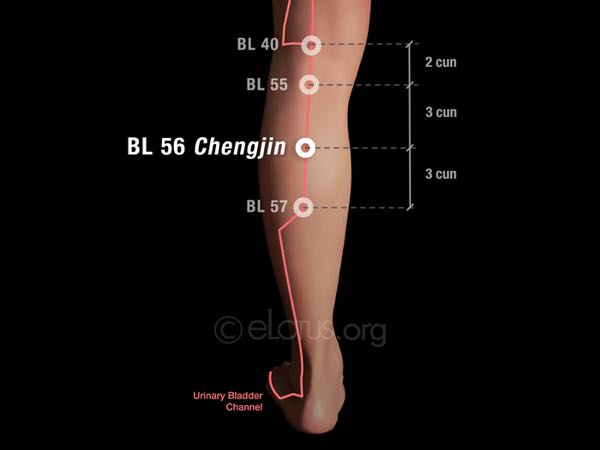
\includegraphics[width=\linewidth]{images/optimized/point_bl56.jpg}\caption{Hình minh họa huyệt BL 56.}\end{figure}
\subsection*{Chỉ định}Đau lưng cấp tính ; Co thắt Vị; Bệnh trĩ;
\subsection*{Ứng dụng}Thư giãn các gân, kích hoạt kinh và giảm đau; Có lợi cho bàn chân và gót chân;
\subsection*{Thủ thuật}Châm thẳng 0,8-1,2 thốn.
\subsection{BL 57 - Thừa Sơn (Chengshan)}
\subsection*{Thông tin cơ bản}\begin{description}\item[Hán tự và phiên âm:] 承山; chéng shān.\item[Ý nghĩa tên (theo tiếng Anh nguồn):] Nâng đỡ núi (dịch sát nghĩa; literal translation); tiếng Anh nguồn: Mountain Support, Support the Mountain.\end{description}
\subsection*{Vị trí}Trên đường giữa sau của chân, giữa Uỷ Trung (BL 40) và Côn Lôn (BL 60), ở chỗ lõm hình thành bên dưới bụng cơ bụng khi cơ bị uốn cong.
\begin{figure}[H]\centering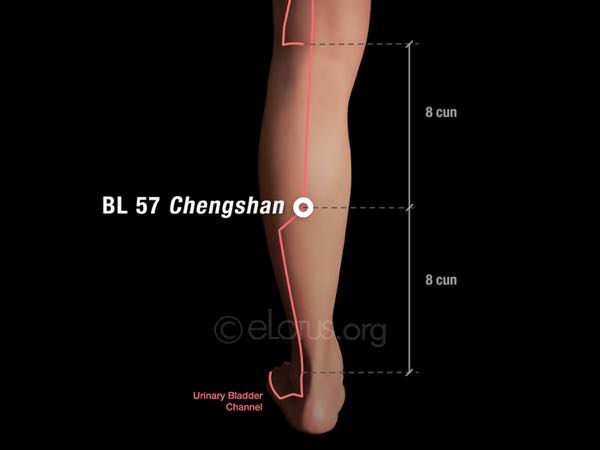
\includegraphics[width=\linewidth]{images/optimized/point_bl57.jpg}\caption{Hình minh họa huyệt BL 57.}\end{figure}
\subsection*{Chỉ định}Đau lưng dưới, co thắt cơ sinh đôi ; Bệnh trĩ, táo bón, beriberi;
\subsection*{Ứng dụng}Thư giãn các gân, kích hoạt kinh và giảm đau; Lợi ích cho bắp chân và gót chân;
\subsection*{Thủ thuật}Châm thẳng 0,8-1,2 thốn.
\subsection{BL 58 - Phi Dương (Feiyang)}
\subsection*{Thông tin cơ bản}\begin{description}\item[Hán tự và phiên âm:] 飛陽; fēi yáng.\item[Ý nghĩa tên (theo tiếng Anh nguồn):] Bay lên (dịch sát nghĩa; literal translation); tiếng Anh nguồn: Taking Flight, Soaring Upwards, Flying Up.\end{description}
\subsection*{Vị trí}7 thốn ngay phía trên Côn Luân (BL 60) , ở bờ sau xương mác, cách khoảng 1 thốn về phía bên và kém hơn Chengshang (BL 57) .
\begin{figure}[H]\centering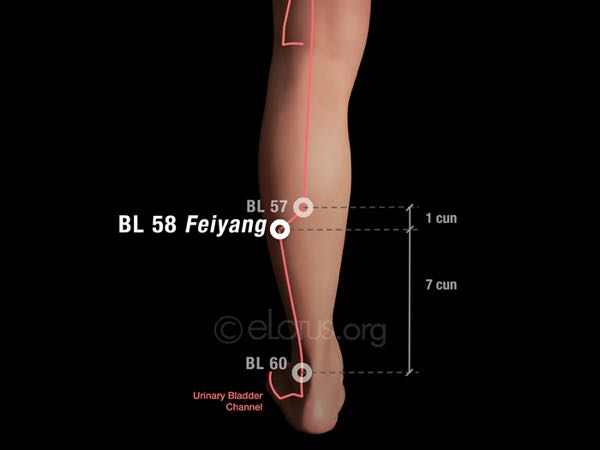
\includegraphics[width=\linewidth]{images/optimized/point_bl58.jpg}\caption{Hình minh họa huyệt BL 58.}\end{figure}
\subsection*{Chỉ định}Nhức đầu, mờ mắt ; Nghẹt mũi, chảy huyết cam; Đau lưng, yếu chân; Bệnh trĩ;
\subsection*{Ứng dụng}Hài hòa phần thân trên và thân dưới ; Xua tan mầm bệnh kinh taiyang; Kích hoạt kinh và giảm đau;
\subsection*{Thủ thuật}Châm thẳng 0,7-1,0 thốn.
\subsection*{Phân loại và ghi chú}Điểm đặc biệt Ghi chú: Điểm kết nối Luo - Bàng Quang
\subsection{BL 59 - Phụ Dương (Fuyang)}
\subsection*{Thông tin cơ bản}\begin{description}\item[Hán tự và phiên âm:] 跗陽; fū yáng.\item[Ý nghĩa tên (theo tiếng Anh nguồn):] Dương ở mu bàn chân (dịch sát nghĩa; literal translation); tiếng Anh nguồn: Instep Yang.\end{description}
\subsection*{Vị trí}3 thốn ngay trên Côn Lôn (BL 60) .
\begin{figure}[H]\centering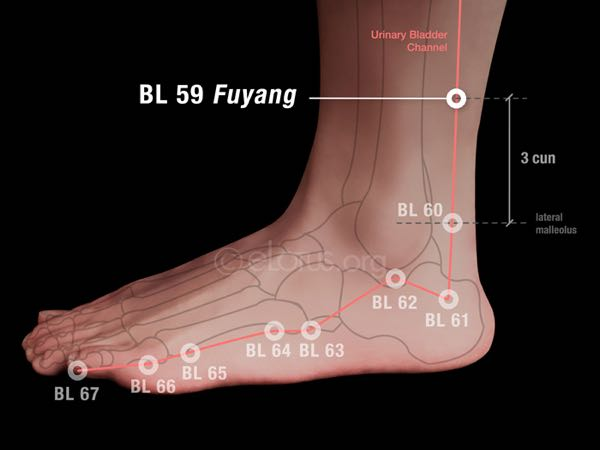
\includegraphics[width=\linewidth]{images/optimized/point_bl59.jpg}\caption{Hình minh họa huyệt BL 59.}\end{figure}
\subsection*{Chỉ định}Cảm giác nặng đầu, đau đầu ; Đau lưng, tê liệt chi dưới; Đỏ và sưng mắt cá ngoài ;
\subsection*{Ứng dụng}Có lợi cho vùng thắt lưng và chân ; Kích hoạt kinh và giảm đau;
\subsection*{Thủ thuật}Châm thẳng 0,5-1,0 thốn.
\subsection*{Phân loại và ghi chú}Phân loại và ghi chú: Khích huyệt - Kinh Yangqiao (Phong trào)
\subsection{BL 60 - Côn Lôn (Kunlun)}
\subsection*{Thông tin cơ bản}\begin{description}\item[Hán tự và phiên âm:] 昆侖; kūn lún.\item[Ý nghĩa tên (theo tiếng Anh nguồn):] Núi Côn Lôn (dịch sát nghĩa; literal translation); tiếng Anh nguồn: Kunlun Mountains.\end{description}
\subsection*{Vị trí}Ở chỗ lõm giữa đầu mắt cá ngoài và gân Achilles.
\begin{figure}[H]\centering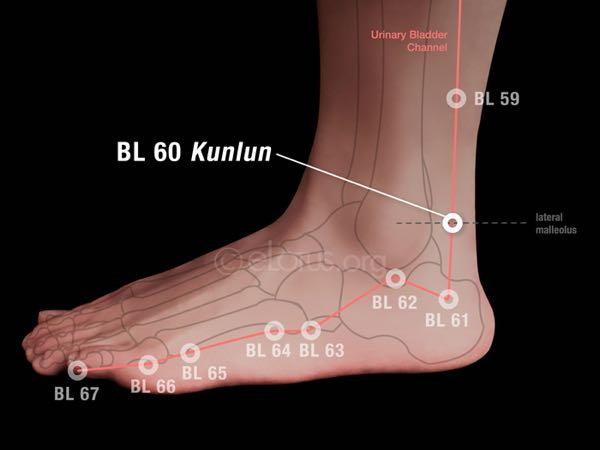
\includegraphics[width=\linewidth]{images/optimized/point_bl60.jpg}\caption{Hình minh họa huyệt BL 60.}\end{figure}
\subsection*{Chỉ định}Nhức đầu, mờ mắt, động kinh, chảy huyết cam ; Đau ở vai, lưng và cánh tay, cứng cổ, sưng và đau gót chân; Lao động khó khăn;
\subsection*{Ứng dụng}Thanh nhiệt, hạ dương, khu phong, hạ dư thừa ; Kích hoạt toàn bộ kinh Bàng Quang tiết niệu và giảm đau; Thư giãn gân cốt, tăng cường sức mạnh cho cột sống thắt lưng; Thúc đẩy lao động;
\subsection*{Thủ thuật}Châm thẳng 0,5-1,0 thốn.
\subsection*{Phân loại và ghi chú}Điểm đặc biệt Ghi chú: Huyệt Kinh (Lửa) - Bàng Quang
\subsection{BL 61 - Bộc Tham (Pucan)}
\subsection*{Thông tin cơ bản}\begin{description}\item[Hán tự và phiên âm:] 僕參; pú cān, pú shēn.\item[Ý nghĩa tên (theo tiếng Anh nguồn):] Khách khiêm nhường (dịch sát nghĩa; literal translation); tiếng Anh nguồn: Subservient Visitor, Servant's Respect, Serve and Consult.\end{description}
\subsection*{Vị trí}Phía sau và kém hơn mắt cá ngoài, ngay dưới Côn Lôn (BL 60), ở chỗ lõm trên xương gót, nơi tiếp giáp giữa da đỏ và da trắng.
\begin{figure}[H]\centering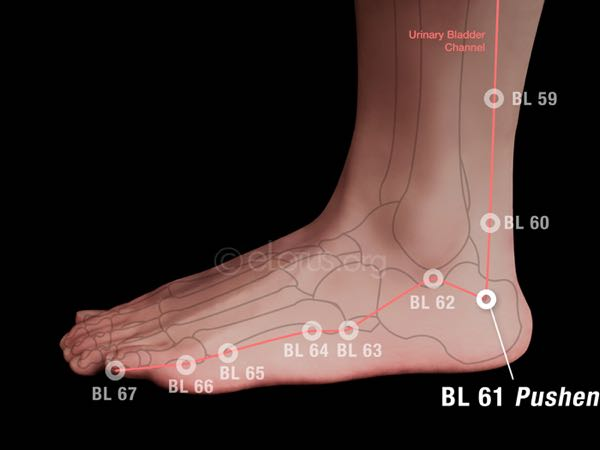
\includegraphics[width=\linewidth]{images/optimized/point_bl61.jpg}\caption{Hình minh họa huyệt BL 61.}\end{figure}
\subsection*{Chỉ định}Teo cơ và yếu chi dưới ; Đau gót chân;
\subsection*{Ứng dụng}Thư giãn các gân, kích hoạt kinh và giảm đau;
\subsection*{Thủ thuật}Châm thẳng 0,3-0,5 thốn.
\subsection{BL 62 - Thân Mạch (Shenmai)}
\subsection*{Thông tin cơ bản}\begin{description}\item[Hán tự và phiên âm:] 申脈; shēn mài.\item[Ý nghĩa tên (theo tiếng Anh nguồn):] Mạch vươn dài (dịch sát nghĩa; literal translation); tiếng Anh nguồn: Extending Vessel, Ninth Channel.\end{description}
\subsection*{Vị trí}Trong chỗ lõm ngay bên dưới mắt cá ngoài, phía sau gân mác.
\begin{figure}[H]\centering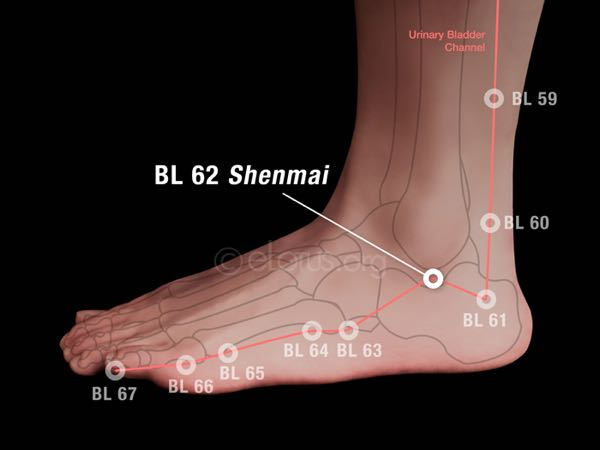
\includegraphics[width=\linewidth]{images/optimized/point_bl62.jpg}\caption{Hình minh họa huyệt BL 62.}\end{figure}
\subsection*{Chỉ định}Nhức đầu, chóng mặt ; Động kinh, hưng cảm, mất ngủ; Đau lưng, đau chân;
\subsection*{Ứng dụng}Khu phong bên trong, đẩy gió bên ngoài ; An thần; Lợi ích đầu và mắt; Mở và điều chỉnh kinh yangqiao (chuyển động); Kích hoạt kinh và giảm đau;
\subsection*{Thủ thuật}Châm thẳng 0,3-0,5 thốn.
\subsection*{Phân loại và ghi chú}Điểm đặc biệt Ghi chú: Điểm Master - Yangqiao (Phong trào) Điểm ghép kinh - Du (Chi phối) Kinh 13 Điểm ma - Đường
\subsection{BL 63 - Kim Môn (Jinmen)}
\subsection*{Thông tin cơ bản}\begin{description}\item[Hán tự và phiên âm:] 金門; jīn mén.\item[Ý nghĩa tên (theo tiếng Anh nguồn):] Cửa Kim (dịch sát nghĩa; literal translation); tiếng Anh nguồn: Metal Gate, Golden Gate, Golden Door.\end{description}
\subsection*{Vị trí}Ở mặt bên của bàn chân, bên dưới bờ trước của mắt cá ngoài, ở bờ dưới của xương hộp, xa lồi củ của xương bàn chân thứ 5.
\begin{figure}[H]\centering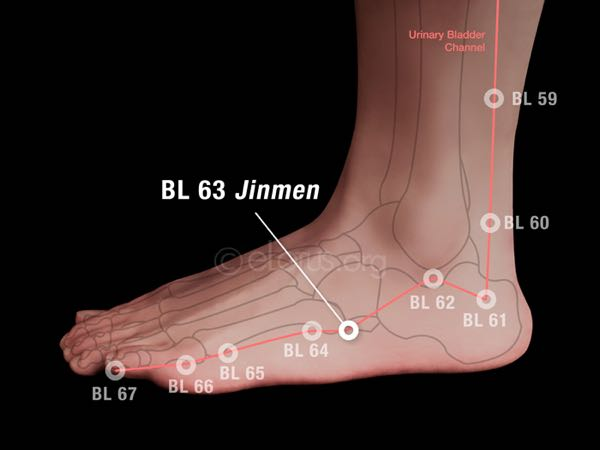
\includegraphics[width=\linewidth]{images/optimized/point_bl63.jpg}\caption{Hình minh họa huyệt BL 63.}\end{figure}
\subsection*{Chỉ định}Chứng hưng cảm, động kinh, co giật ở trẻ sơ sinh ; Đau lưng, đau mắt cá chân; Suy giảm vận động và đau chi dưới;
\subsection*{Ứng dụng}Khu phong ; Điều kiện cấp tính vừa phải; Thư giãn các gân, kích hoạt kinh mạch và giảm đau;
\subsection*{Thủ thuật}Châm thẳng 0,3-0,5 thốn.
\subsection*{Phân loại và ghi chú}Điểm đặc biệt Ghi chú: Khích huyệt - Bàng Quang
\subsection{BL 64 - Kinh Cốt (Jinggu)}
\subsection*{Thông tin cơ bản}\begin{description}\item[Hán tự và phiên âm:] 京骨; jīng gǔ.\item[Ý nghĩa tên (theo tiếng Anh nguồn):] Xương kinh (dịch sát nghĩa; literal translation); tiếng Anh nguồn: Capital Bone.\end{description}
\subsection*{Vị trí}Trong chỗ lõm bên dưới củ của xương bàn chân thứ 5, tại điểm nối của da đỏ và da trắng.
\begin{figure}[H]\centering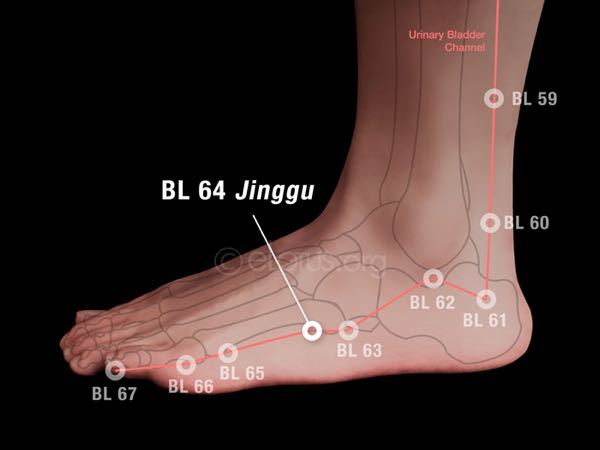
\includegraphics[width=\linewidth]{images/optimized/point_bl64.jpg}\caption{Hình minh họa huyệt BL 64.}\end{figure}
\subsection*{Chỉ định}Nhức đầu, cứng cổ ; Động kinh; Đau vùng lưng dưới và đùi;
\subsection*{Ứng dụng}Làm sạch đầu, mắt và khu phong ; An thần; Thư giãn các gân, kích hoạt kinh mạch và giảm đau;
\subsection*{Thủ thuật}Châm thẳng 0,3-0,5 thốn.
\subsection*{Phân loại và ghi chú}Điểm đặc biệt Ghi chú: Điểm nguồn Yuan - Bàng Quang
\subsection{BL 65 - Thúc Cốt (Shugu)}
\subsection*{Thông tin cơ bản}\begin{description}\item[Hán tự và phiên âm:] 束骨; shù gǔ.\item[Ý nghĩa tên (theo tiếng Anh nguồn):] Xương bó lại (dịch sát nghĩa; literal translation); tiếng Anh nguồn: Bundle Bone, Restraining Bone, Binding Bone.\end{description}
\subsection*{Vị trí}Trong chỗ lõm gần khớp bàn chân thứ 5, tại điểm nối của da đỏ và da trắng.
\begin{figure}[H]\centering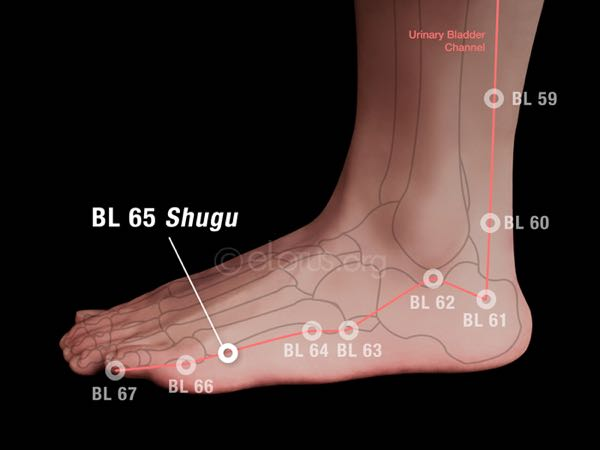
\includegraphics[width=\linewidth]{images/optimized/point_bl65.jpg}\caption{Hình minh họa huyệt BL 65.}\end{figure}
\subsection*{Chỉ định}Nhức đầu, cứng cổ ; Hưng cảm, mờ mắt; Đau lưng, đau nhức chi dưới;
\subsection*{Ứng dụng}Xóa đầu và mắt ; Thanh nhiệt, tiêu sưng, trừ gió; Kích hoạt kinh và giảm đau;
\subsection*{Thủ thuật}Châm thẳng 0,3-0,5 thốn.
\subsection*{Phân loại và ghi chú}Điểm đặc biệt nhận xét: Điểm suối Shu (Mộc) - Bàng Quang
\subsection{BL 66 - Túc Thông Cốc (Zutonggu)}
\subsection*{Thông tin cơ bản}\begin{description}\item[Hán tự và phiên âm:] 足通谷; zú tōng gǔ.\item[Ý nghĩa tên (theo tiếng Anh nguồn):] Thung lũng thông ở bàn chân (dịch sát nghĩa; literal translation); tiếng Anh nguồn: Valley Passage, Foot Connecting Valley, Passing Valley of the Foot.\end{description}
\subsection*{Vị trí}Trong chỗ lõm xa đến khớp bàn chân thứ 5, tại điểm nối của da đỏ và da trắng.
\begin{figure}[H]\centering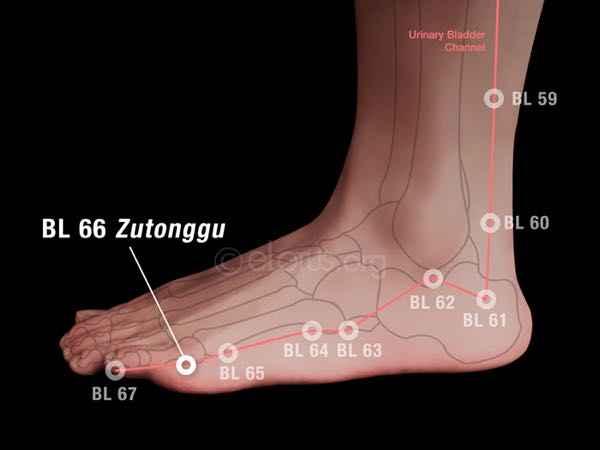
\includegraphics[width=\linewidth]{images/optimized/point_bl66.jpg}\caption{Hình minh họa huyệt BL 66.}\end{figure}
\subsection*{Chỉ định}Nhức đầu, cứng cổ ; Mờ mắt, chảy huyết cam; hưng cảm ;
\subsection*{Ứng dụng}Làm sạch đầu, trục gió, thanh nhiệt; Đi xuống khí Phế và Vị;
\subsection*{Thủ thuật}Châm thẳng 0,2-0,3 thốn.
\subsection*{Phân loại và ghi chú}Điểm đặc biệt Ghi chú: Điểm suối Ying (Nước) - Bàng Quang

\clearpage
\section{Kinh Túc Thiếu Âm Thận}
\begin{description}
\item[Tên kinh/mạch:] Kinh Túc Thiếu Âm Thận (Thận) .
\item[Hán tự và phiên âm:] 足少陰腎經; zú shào yīn shèn jīng.
\item[Thời gian hoạt động:] 5--7 giờ chiều.
\item[Ngũ hành:] Thủy.
\item[Kinh biểu lý:] Túc Thái Dương Bàng Quang.
\end{description}
\subsection*{Đường đi và phạm vi}Kinh mạch Thận bắt nguồn từ dưới ngón chân út và chạy ngang lòng bàn chân đến Yong Tuyền (KI 1) . Nó xuất phát từ mặt dưới của củ xương thuyền, vòng ra phía sau mắt cá trong và đi qua gót chân. Sau đó, kinh đi lên dọc theo mặt trong của đùi, đi qua Tam Âm Giao (SP 6), đến mặt trong của hố khoeo và tiếp tục đi lên dọc theo mặt sau trong của đùi về phía gốc cột sống tại Trường Cường (GV 1), nơi kinh đi vào cơ quan Thận và kết nối với Bàng Quang. Sau đó nó quay trở lại bề mặt bụng phía trên xương mu và chạy lên trên bụng, xuyên qua Trung Cực (CV 3) và Quan Nguyên (CV 4), xuyên qua ngực. Nhánh thẳng tái xuất hiện từ cơ quan Thận. Đi lên và đi qua Can và cơ hoành, kinh đi vào Phế, chạy dọc theo cổ họng và kết thúc ở gốc lưỡi. Một nhánh khác xuất hiện từ Phế, nối với Tâm và chảy vào rương, nơi nó kết nối với kinh Tâm Bào.
\subsection*{Chỉ định của kinh/mạch}Đi tiểu thường xuyên, bất lực ; Kinh nguyệt không đều, lạnh chân;
\subsection*{Ứng dụng của kinh/mạch}Lưu trữ Tinh chất ; Thống trị sự sinh sản và phát triển của con người; Tạo ra tủy; Quản lý nước; Kiểm soát việc tiếp nhận Qi; Thống trị xương; Sản xuất huyết; Mở vào tai; Biểu hiện ở tóc; Kiểm soát hai lỗ dưới; Nhà Ý Chí (Zhi) ;
\subsection*{Phương pháp cân bằng}
\begin{enumerate}
\item Kinh Thủ Thiếu Âm Tâm.
\item Kinh Thủ Thiếu Dương Tam Tiêu.
\item Kinh Túc Thái Dương Bàng Quang.
\item Kinh Thủ Dương Minh Đại Trường.
\item Kinh Thủ Quyết Âm Tâm Bào.
\end{enumerate}
\subsection*{Các huyệt đặc biệt}
\begin{itemize}
\item Tỉnh (Jing-Well): Dũng Tuyền (KI1).
\item Huỳnh (Ying-Spring): Nhiên Cốc (KI2).
\item Du (Shu-Stream): Thái Khê (KI3).
\item Kinh (Jing-River): Phục Lưu (KI7).
\item Hợp (He-Sea): Âm Cốc (KI10).
\item Nguyên huyệt: Thái Khê (KI3).
\item Lạc huyệt: Đại Chung (KI4).
\item Khích huyệt: Thuỷ Tuyền (KI5).
\item Mộ huyệt trước: Kinh Môn (GB25).
\item Du huyệt sau: Thận Du (BL23).
\item Huyệt Mẹ: Phục Lưu (KI7).
\item Huyệt Con: Dũng Tuyền (KI1).
\item Huyệt Nhập: Dũng Tuyền (KI1).
\item Huyệt Xuất: Bộ Lang (KI22).
\end{itemize}
\subsection{KI 1 - Dũng Tuyền (Yongquan)}
\subsection*{Thông tin cơ bản}\begin{description}\item[Hán tự và phiên âm:] 涌泉; yǒng quán.\item[Ý nghĩa tên (theo tiếng Anh nguồn):] Suối phun trào (dịch sát nghĩa; literal translation); tiếng Anh nguồn: Gushing Spring, Bubbling Well, Bubbling Spring.\end{description}
\subsection*{Vị trí}Ở lòng bàn chân, với bàn chân ở tư thế gấp lòng bàn chân, điểm này nằm ở chỗ lõm giữa xương bàn chân thứ 2 và thứ 3, gần như ở điểm nối của 1/3 trước và 2/3 sau của đường nối gốc ngón chân thứ 2 và thứ 3 với gót chân.
\begin{figure}[H]\centering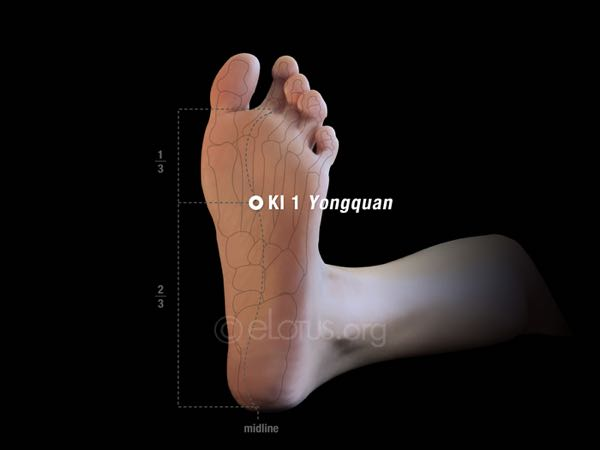
\includegraphics[width=\linewidth]{images/optimized/point_ki1.jpg}\caption{Hình minh họa huyệt KI 1.}\end{figure}
\subsection*{Chỉ định}Nhức đầu, mờ mắt, chóng mặt ; Đau họng, khô lưỡi, mất giọng; Co giật ở trẻ sơ sinh, mất ý thức; Cảm giác sốt ở lòng bàn chân, tiểu khó;
\subsection*{Ứng dụng}Đi xuống phần thừa từ đầu ; An thần; Phục hồi ý thức, cứu dương;
\subsection*{Thủ thuật}Châm thẳng 0,3-0,5 thốn.
\subsection*{Phân loại và ghi chú}Điểm đặc biệt Ghi chú: Huyệt Tỉnh (Gỗ) - Thận Huyệt Nhập - Thận
\subsection{KI 2 - Nhiên Cốc (Rangu)}
\subsection*{Thông tin cơ bản}\begin{description}\item[Hán tự và phiên âm:] 然谷; rán gǔ.\item[Ý nghĩa tên (theo tiếng Anh nguồn):] Thung lũng rực cháy (dịch sát nghĩa; literal translation); tiếng Anh nguồn: Blazing Valley.\end{description}
\subsection*{Vị trí}Phía trước và dưới mắt cá trong, ở chỗ lõm ở bờ dưới của củ xương thuyền.
\begin{figure}[H]\centering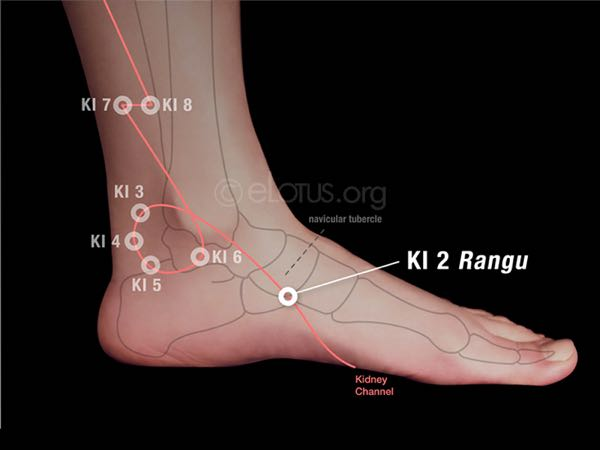
\includegraphics[width=\linewidth]{images/optimized/point_ki2.jpg}\caption{Hình minh họa huyệt KI 2.}\end{figure}
\subsection*{Chỉ định}Ho ra huyết, khát nước, tiêu chảy ; Ngứa âm hộ, sa tử thống, kinh nguyệt không đều, xuất tinh về đêm; Sưng và đau ở mu bàn chân; Viêm rốn cấp tính ở trẻ sơ sinh;
\subsection*{Ứng dụng}Xóa nhiệt thiếu hụt; Điều hòa Thận; Điều chỉnh jiao dưới ;
\subsection*{Thủ thuật}Châm thẳng 0,3-0,5 thốn.
\subsection*{Phân loại và ghi chú}Điểm đặc biệt Ghi chú: Điểm lò xo Ying (Lửa) - Thận
\subsection{KI 3 - Thái Khê (Taixi)}
\subsection*{Thông tin cơ bản}\begin{description}\item[Hán tự và phiên âm:] 太谿; taì xī.\item[Ý nghĩa tên (theo tiếng Anh nguồn):] Khe lớn (dịch sát nghĩa; literal translation); tiếng Anh nguồn: Great Ravine, Supreme Stream, Greater Stream.\end{description}
\subsection*{Vị trí}Ở chỗ lõm giữa đầu mắt cá trong và gân Achilles.
\begin{figure}[H]\centering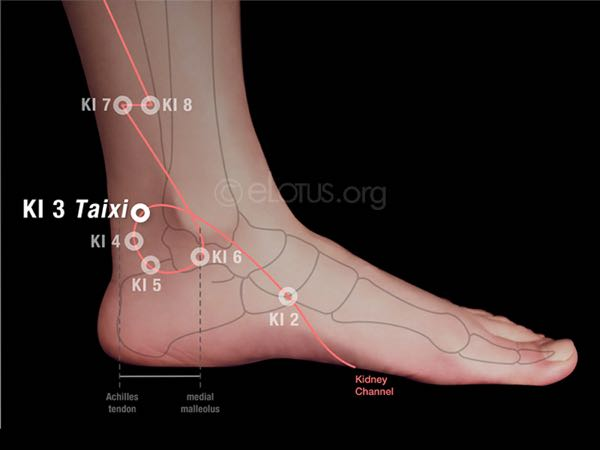
\includegraphics[width=\linewidth]{images/optimized/point_ki3.jpg}\caption{Hình minh họa huyệt KI 3.}\end{figure}
\subsection*{Chỉ định}Đau họng, đau răng, khạc ra huyết, khát nước ; Điếc, ù tai, chóng mặt, hen suyễn; Kinh nguyệt không đều, xuất tinh về đêm, bất lực, tiểu nhiều lần; Đau lưng dưới; Mất ngủ;
\subsection*{Ứng dụng}Bồi bổ Thận âm, thanh nhiệt thiếu hụt; Tăng cường Thận dương; Neo khí ; Tăng cường cột sống thắt lưng;
\subsection*{Thủ thuật}Châm thẳng 0,3-0,5 thốn.
\subsection*{Phân loại và ghi chú}Điểm đặc biệt Ghi chú: Điểm suối Shu (Trái đất) - Điểm nguồn Thận Yuan - Thận
\subsection{KI 4 - Đại Chung (Dazhong)}
\subsection*{Thông tin cơ bản}\begin{description}\item[Hán tự và phiên âm:] 大鐘; dà zhōng.\item[Ý nghĩa tên (theo tiếng Anh nguồn):] Chuông lớn (dịch sát nghĩa; literal translation); tiếng Anh nguồn: Large Goblet, Great Bell, Big Bell.\end{description}
\subsection*{Vị trí}Phía sau và dưới mắt cá trong, ở chỗ lõm phía trước mặt trong của chỗ bám gân Achilles.
\begin{figure}[H]\centering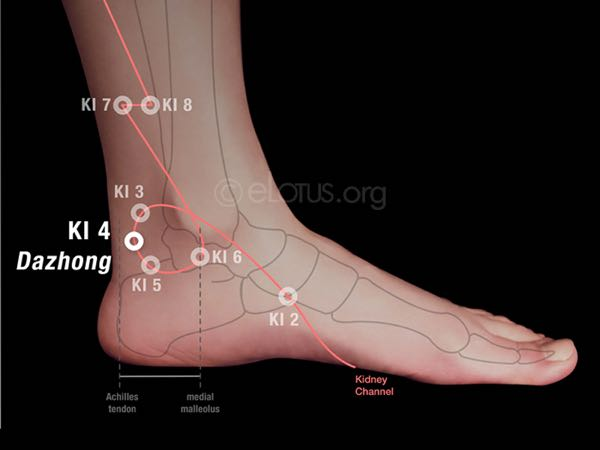
\includegraphics[width=\linewidth]{images/optimized/point_ki4.jpg}\caption{Hình minh họa huyệt KI 4.}\end{figure}
\subsection*{Chỉ định}Tiểu khó, táo bón ; Khạc nhổ hoặc ho ra huyết, hen suyễn; Đau lưng dưới và cứng khớp, đau gót chân; Chứng mất trí nhớ;
\subsection*{Ứng dụng}Tăng cường Thận ; Neo khí, lợi Phế ; Tăng cường ý chí, xua tan nỗi sợ hãi;
\subsection*{Thủ thuật}Châm thẳng 0,3-0,5 thốn.
\subsection*{Phân loại và ghi chú}Điểm đặc biệt Ghi chú: Điểm kết nối Luo - Thận
\subsection{KI 5 - Thuỷ Tuyền (Shuiquan)}
\subsection*{Thông tin cơ bản}\begin{description}\item[Hán tự và phiên âm:] 水泉; shuǐ quán.\item[Ý nghĩa tên (theo tiếng Anh nguồn):] Suối nước (dịch sát nghĩa; literal translation); tiếng Anh nguồn: Water Spring.\end{description}
\subsection*{Vị trí}1 thốn ngay bên dưới Thái Khê h Tu (KI 3), trong chỗ lõm ở phía trong của lồi củ xương gót.
\begin{figure}[H]\centering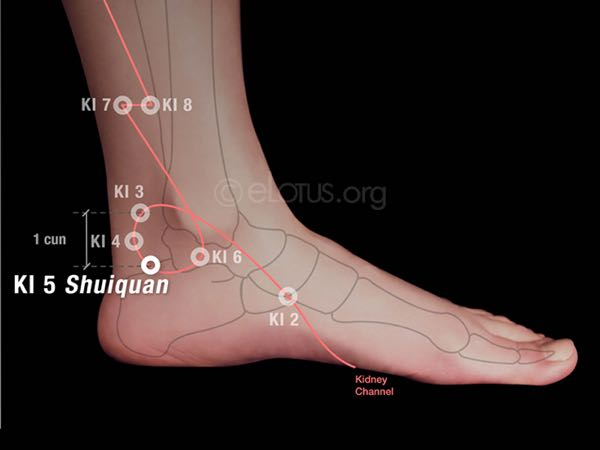
\includegraphics[width=\linewidth]{images/optimized/point_ki5.jpg}\caption{Hình minh họa huyệt KI 5.}\end{figure}
\subsection*{Chỉ định}Vô kinh, kinh nguyệt không đều, đau bụng kinh ; Sa tử thống, tiểu khó; Làm mờ tầm nhìn;
\subsection*{Ứng dụng}Điều chỉnh kinh chong (đường phố) và mạch Nhâm (hình thành); Lợi ích kinh nguyệt;
\subsection*{Thủ thuật}Châm thẳng 0,3-0,5 thốn.
\subsection*{Phân loại và ghi chú}Điểm đặc biệt Ghi chú: Khích huyệt - Thận
\subsection{KI 6 - Chiếu Hải (Zhaohai)}
\subsection*{Thông tin cơ bản}\begin{description}\item[Hán tự và phiên âm:] 照海; zhào hǎi.\item[Ý nghĩa tên (theo tiếng Anh nguồn):] Biển sáng (dịch sát nghĩa; literal translation); tiếng Anh nguồn: Shining Sea.\end{description}
\subsection*{Vị trí}Trong chỗ lõm bên dưới đầu mắt cá trong.
\begin{figure}[H]\centering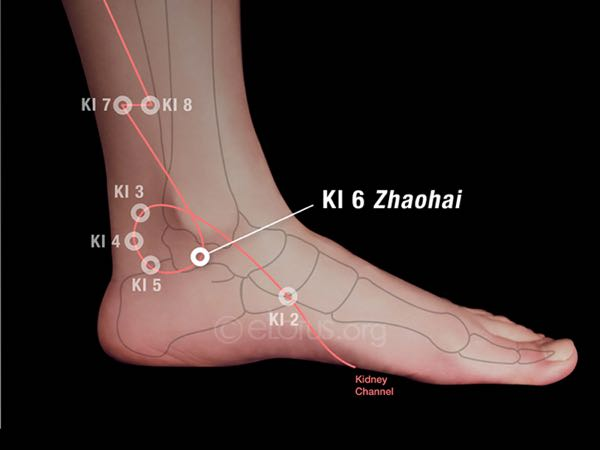
\includegraphics[width=\linewidth]{images/optimized/point_ki6.jpg}\caption{Hình minh họa huyệt KI 6.}\end{figure}
\subsection*{Chỉ định}Viêm họng, hen suyễn ; Tần suất đi tiểu, bí tiểu, táo bón; Động kinh, mất ngủ; Kinh nguyệt không đều, bệnh bạch cầu, sa tử thống, ngứa âm hộ;
\subsection*{Ứng dụng}Lợi ích cho cổ họng ; Bổ Thận, thanh nhiệt thiếu hụt; Điều chỉnh kinh âm kiều (chuyển động); An thần; Điều chỉnh jiao dưới ;
\subsection*{Thủ thuật}Châm thẳng 0,3-0,5 thốn.
\subsection*{Phân loại và ghi chú}Điểm đặc biệt Ghi chú: Điểm chính - Kinh Yinqiao (Chuyển động) Điểm kết hợp - mạch Nhâm (Quan niệm)
\subsection{KI 7 - Phục Lưu (Fuliu)}
\subsection*{Thông tin cơ bản}\begin{description}\item[Hán tự và phiên âm:] 復溜; fù liū.\item[Ý nghĩa tên (theo tiếng Anh nguồn):] Dòng chảy quay lại (dịch sát nghĩa; literal translation); tiếng Anh nguồn: Recover Flow, Returning Current.\end{description}
\subsection*{Vị trí}2 thốn ngay trên Thái Khê h Tu (KI 3), ở bờ trước của gân Achilles.
\begin{figure}[H]\centering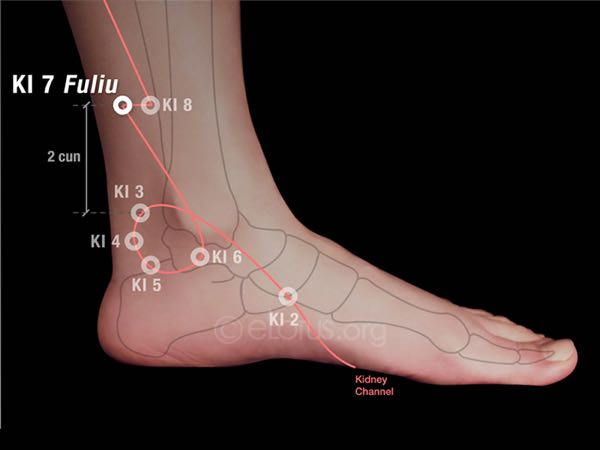
\includegraphics[width=\linewidth]{images/optimized/point_ki7.jpg}\caption{Hình minh họa huyệt KI 7.}\end{figure}
\subsection*{Chỉ định}Chướng bụng, tiêu chảy, chán ăn ; Đổ mồ hôi đêm, đổ mồ hôi tự phát, bệnh sốt không ra mồ hôi; Teo cơ chân, phù nề;
\subsection*{Ứng dụng}Có lợi cho Thận ; Điều hòa đường dẫn nước, điều tiết mồ hôi; Thoát ẩm, giải nhiệt; Tăng cường vùng thắt lưng;
\subsection*{Thủ thuật}Châm thẳng 0,5-0,7 thốn.
\subsection*{Phân loại và ghi chú}Điểm đặc biệt Ghi chú: Huyệt Kinh (Kim loại) - Thận
\subsection{KI 8 - Giao Tín (Jiaoxin)}
\subsection*{Thông tin cơ bản}\begin{description}\item[Hán tự và phiên âm:] 交信; jiāo xìn.\item[Ý nghĩa tên (theo tiếng Anh nguồn):] Giao điểm của sự tin cậy (dịch sát nghĩa; literal translation); tiếng Anh nguồn: Intersection Reach, Exchange Belief.\end{description}
\subsection*{Vị trí}2 thốn trên Thái Khê h Tu (KI 3), 0,5 thốn trước Phục Lưu (KI 7), sau bờ trong xương chày.
\begin{figure}[H]\centering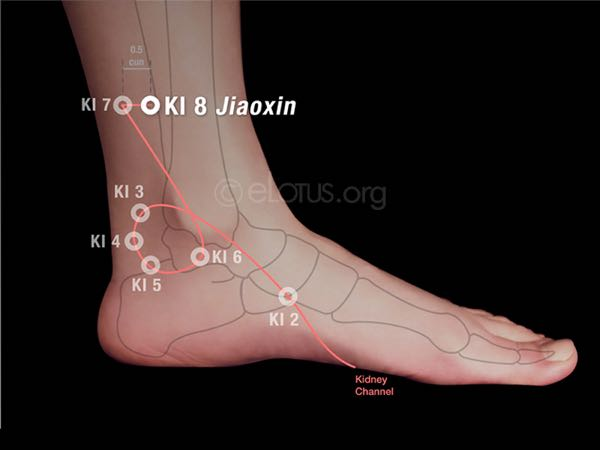
\includegraphics[width=\linewidth]{images/optimized/point_ki8.jpg}\caption{Hình minh họa huyệt KI 8.}\end{figure}
\subsection*{Chỉ định}Chảy huyết tử thống, sa tử thống ; Kinh nguyệt không đều, đau bụng kinh; Tiêu chảy, táo bón; Đau và sưng tinh hoàn;
\subsection*{Ứng dụng}Điều chỉnh các tàu ren (thụ thai) và chong (đường lộ); Điều hòa kinh nguyệt; Làm sạch nhiệt và thoát ẩm từ jiao phía dưới;
\subsection*{Thủ thuật}Châm thẳng 0,5-0,7 thốn.
\subsection*{Phân loại và ghi chú}Phân loại và ghi chú: Khích huyệt - Yinqiao (Movement) Channel
\subsection{KI 9 - Trúc Tân (Zhubin)}
\subsection*{Thông tin cơ bản}\begin{description}\item[Hán tự và phiên âm:] 築賓; zhú bīn.\item[Ý nghĩa tên (theo tiếng Anh nguồn):] Nhà khách (dịch sát nghĩa; literal translation); tiếng Anh nguồn: Guest House, Guest Building.\end{description}
\subsection*{Vị trí}5 thốn ngay phía trên Thái Khê h Tu (KI 3) ở đầu dưới bụng của cơ bụng chân, trên đường kéo từ Thái Khê h Tu (KI 3) đến Yingu (Thận l0), cách bờ trong xương chày khoảng 1 thốn.
\begin{figure}[H]\centering\includegraphics[width=\linewidth]{images/optimized/point_ki9.jpg}\caption{Hình minh họa huyệt KI 9.}\end{figure}
\subsection*{Chỉ định}Rối loạn tâm thần ; Đau ở bàn chân và cẳng chân; Thoát vị ;
\subsection*{Ứng dụng}Làm sạch tim, chuyển hóa đờm ; Điều hòa khí, giảm đau;
\subsection*{Thủ thuật}Châm thẳng 0,5-0,7 thốn.
\subsection*{Phân loại và ghi chú}Phân loại và ghi chú: Khích huyệt - Kinh Yinwei (Liên kết)
\subsection{KI 10 - Âm Cốc (Yingu)}
\subsection*{Thông tin cơ bản}\begin{description}\item[Hán tự và phiên âm:] 陰谷; yīn gǔ.\item[Ý nghĩa tên (theo tiếng Anh nguồn):] Thung lũng Âm (dịch sát nghĩa; literal translation); tiếng Anh nguồn: Yin Valley.\end{description}
\subsection*{Vị trí}Với đầu gối gập lại, điểm nằm ở phía trong của nếp gấp khoeo, giữa các gân của cơ bán gân và cơ bán màng, ngang mức với Uỷ Trung (BL 40) .
\begin{figure}[H]\centering\includegraphics[width=\linewidth]{images/optimized/point_ki10.jpg}\caption{Hình minh họa huyệt KI 10.}\end{figure}
\subsection*{Chỉ định}Bất lực, chảy huyết tử thống, tiểu khó ; Thoát vị, đau đầu gối và hố khoeo ; Rối loạn tâm thần;
\subsection*{Ứng dụng}Loại bỏ nhiệt ẩm từ jiao phía dưới ; Lợi ích Thận; Kích hoạt kinh và giảm đau;
\subsection*{Thủ thuật}Châm thẳng 0,8-1,0 thốn.
\subsection*{Phân loại và ghi chú}Điểm đặc biệt nhận xét: He Huyệt Hải (Nước) - Thận
\subsection{KI 11 - Hoành Cốt (Henggu)}
\subsection*{Thông tin cơ bản}\begin{description}\item[Hán tự và phiên âm:] 橫骨; héng gǔ.\item[Ý nghĩa tên (theo tiếng Anh nguồn):] Xương ngang (dịch sát nghĩa; literal translation); tiếng Anh nguồn: Public Bone, Horizontal Bone.\end{description}
\subsection*{Vị trí}5 thốn dưới rốn, trên bờ trên của khớp mu, 0,5 thốn phía ngoài so với Khúc Cốt (CV 2) .
\begin{figure}[H]\centering\includegraphics[width=\linewidth]{images/optimized/point_ki11.jpg}\caption{Hình minh họa huyệt KI 11.}\end{figure}
\subsection*{Chỉ định}Đầy bụng và đau bụng dưới ; Tiểu khó, đái dầm, tiểu đêm, liệt dương; Đau cơ quan sinh dục;
\subsection*{Ứng dụng}Mang lại lợi ích cho jiao thấp hơn ;
\subsection*{Thủ thuật}Châm thẳng 0,5-1,0 thốn.
\subsection{KI 12 - Đại Hách (Dahe)}
\subsection*{Thông tin cơ bản}\begin{description}\item[Hán tự và phiên âm:] 大赫; dà hè.\item[Ý nghĩa tên (theo tiếng Anh nguồn):] Sự hiển lộ lớn (dịch sát nghĩa; literal translation); tiếng Anh nguồn: Great Manifestation, Great Luminance, Great Clarity.\end{description}
\subsection*{Vị trí}4 thốn dưới rốn, 0,5 thốn về phía ngoài so với Trung Cực (CV 3) .
\begin{figure}[H]\centering\includegraphics[width=\linewidth]{images/optimized/point_ki12.jpg}\caption{Hình minh họa huyệt KI 12.}\end{figure}
\subsection*{Chỉ định}Xuất tinh về đêm, bất lực ; Đau cơ quan sinh dục ngoài, bệnh bạch cầu, sa tử thống;
\subsection*{Ứng dụng}Bổ Thận, làm se tinh chất ;
\subsection*{Thủ thuật}Châm thẳng 0,5-1,0 thốn.
\subsection{KI 13 - Khí Huyệt (Qixue)}
\subsection*{Thông tin cơ bản}\begin{description}\item[Hán tự và phiên âm:] 氣穴; qì xué.\item[Ý nghĩa tên (theo tiếng Anh nguồn):] Hốc Khí (dịch sát nghĩa; literal translation); tiếng Anh nguồn: Qi Hole, Qi Cave.\end{description}
\subsection*{Vị trí}3 thốn dưới rốn, 0,5 thốn về phía ngoài Quan Nguyên (CV 4) .
\begin{figure}[H]\centering\includegraphics[width=\linewidth]{images/optimized/point_ki13.jpg}\caption{Hình minh họa huyệt KI 13.}\end{figure}
\subsection*{Chỉ định}Kinh nguyệt không đều, đau bụng kinh ; Tiểu khó, đau bụng, tiêu chảy;
\subsection*{Ứng dụng}Điều chỉnh kinh chong (đường phố) và mạch Nhâm (hình thành); Điều chỉnh jiao dưới ;
\subsection*{Thủ thuật}Châm thẳng 0,5-1,0 thốn.
\subsection{KI 14 - Tứ Mãn (Siman)}
\subsection*{Thông tin cơ bản}\begin{description}\item[Hán tự và phiên âm:] 四滿; sì mǎn.\item[Ý nghĩa tên (theo tiếng Anh nguồn):] Đầy đủ bốn phương (dịch sát nghĩa; literal translation); tiếng Anh nguồn: Fourfold Fullness, Four Fullness.\end{description}
\subsection*{Vị trí}2 thốn dưới rốn, 0,5 thốn về phía bên so với Thạch Môn (CV 5) .
\begin{figure}[H]\centering\includegraphics[width=\linewidth]{images/optimized/point_ki14.jpg}\caption{Hình minh họa huyệt KI 14.}\end{figure}
\subsection*{Chỉ định}Đau bụng, chướng bụng, tiêu chảy ; Phát thải về đêm; Kinh nguyệt không đều, đau bụng kinh, đau bụng sau sinh;
\subsection*{Ứng dụng}Có lợi cho tiêu dưới, giảm đau; Điều hòa khí huyết ứ ; Điều hòa đường dẫn nước và thúc đẩy đi tiểu;
\subsection*{Thủ thuật}Châm thẳng 0,5-1,0 thốn. Không nên đưa sâu vào vì nó có thể xuyên qua khoang phúc mạc.
\subsection{KI 15 - Trung Chú (Zhongzhu)}
\subsection*{Thông tin cơ bản}\begin{description}\item[Hán tự và phiên âm:] 中注; zhōng zhù.\item[Ý nghĩa tên (theo tiếng Anh nguồn):] Dòng chảy ở giữa (dịch sát nghĩa; literal translation); tiếng Anh nguồn: Central Flow, Middle Flow.\end{description}
\subsection*{Vị trí}1 thốn dưới rốn, 0,5 thốn về phía Âm Giao (CV 7) .
\begin{figure}[H]\centering\includegraphics[width=\linewidth]{images/optimized/point_ki15.jpg}\caption{Hình minh họa huyệt KI 15.}\end{figure}
\subsection*{Chỉ định}Kinh nguyệt không đều ; Đau bụng, táo bón;
\subsection*{Ứng dụng}Điều hòa đường ruột ; Điều chỉnh jiao dưới ;
\subsection*{Thủ thuật}Châm thẳng 0,5-1,0 thốn. Không nên đưa sâu vào vì nó có thể xuyên qua khoang phúc mạc.
\subsection{KI 16 - Hoang Du (Huangshu)}
\subsection*{Thông tin cơ bản}\begin{description}\item[Hán tự và phiên âm:] 肓俞; huāng shū.\item[Ý nghĩa tên (theo tiếng Anh nguồn):] Du huyệt Hoang (dịch sát nghĩa; literal translation); tiếng Anh nguồn: Vitals Shu, Vitals Transporting Point.\end{description}
\subsection*{Vị trí}0,5 thốn về phía ngoài rốn, ngang với Thần Khuyết (CV 8) .
\begin{figure}[H]\centering\includegraphics[width=\linewidth]{images/optimized/point_ki16.jpg}\caption{Hình minh họa huyệt KI 16.}\end{figure}
\subsection*{Chỉ định}Đau bụng, chướng bụng ; Nôn mửa, tiêu chảy, táo bón;
\subsection*{Ứng dụng}Điều hòa khí, giảm đau; Điều hòa Vị và ruột;
\subsection*{Thủ thuật}Châm thẳng 0,5-1,0 thốn. Không nên đưa sâu vào vì nó có thể xuyên qua khoang phúc mạc.
\subsection{KI 17 - Thương Khúc (Shangqu)}
\subsection*{Thông tin cơ bản}\begin{description}\item[Hán tự và phiên âm:] 商曲; shāng qū.\item[Ý nghĩa tên (theo tiếng Anh nguồn):] Khúc quanh Thương (dịch sát nghĩa; literal translation); tiếng Anh nguồn: Shang Bend, Trade Bend.\end{description}
\subsection*{Vị trí}2 thốn phía trên rốn, 0,5 thốn về phía bên ngoài Hạ Loan (CV 10) .
\begin{figure}[H]\centering\includegraphics[width=\linewidth]{images/optimized/point_ki17.jpg}\caption{Hình minh họa huyệt KI 17.}\end{figure}
\subsection*{Chỉ định}Đau bụng, táo bón, tiêu chảy ;
\subsection*{Ứng dụng}Xua tan sự tích tụ, giảm đau;
\subsection*{Thủ thuật}Châm thẳng 0,5-1,0 thốn. Không nên đưa sâu vào vì nó có thể xuyên qua khoang phúc mạc.
\subsection{KI 18 - Thạch Quan (Shiguan)}
\subsection*{Thông tin cơ bản}\begin{description}\item[Hán tự và phiên âm:] 石關; shí guān.\item[Ý nghĩa tên (theo tiếng Anh nguồn):] Cửa đá (dịch sát nghĩa; literal translation); tiếng Anh nguồn: Stone Pass, Stone Hinge.\end{description}
\subsection*{Vị trí}cách rốn 3 thốn, cách Jianli 0,5 thốn (CV 11) .
\begin{figure}[H]\centering\includegraphics[width=\linewidth]{images/optimized/point_ki18.jpg}\caption{Hình minh họa huyệt KI 18.}\end{figure}
\subsection*{Chỉ định}Đau bụng sau sinh, vô sinh ; Nôn, đau bụng, táo bón;
\subsection*{Ứng dụng}Điều hòa tiêu dưới, giảm đau; Điều hòa khí huyết, hoạt huyết ứ; Điều hòa Vị;
\subsection*{Thủ thuật}Châm thẳng 0,5-1,0 thốn. Không nên đưa sâu vào vì nó có thể xuyên qua khoang phúc mạc.
\subsection{KI 19 - Âm Đô (Yindu)}
\subsection*{Thông tin cơ bản}\begin{description}\item[Hán tự và phiên âm:] 陰都; yīn dū.\item[Ý nghĩa tên (theo tiếng Anh nguồn):] Kinh đô Âm (dịch sát nghĩa; literal translation); tiếng Anh nguồn: Yin Metropolis, Yin City.\end{description}
\subsection*{Vị trí}cách rốn 4 thốn, cách Trung Loan 0,5 thốn (CV 12) .
\begin{figure}[H]\centering\includegraphics[width=\linewidth]{images/optimized/point_ki19.jpg}\caption{Hình minh họa huyệt KI 19.}\end{figure}
\subsection*{Chỉ định}Đau bụng, đau vùng thượng vị, táo bón, nôn mửa, borborygmus ; Ho, thở khò khè;
\subsection*{Ứng dụng}Điều hòa khí, điều hòa Vị; Giảm khí nổi loạn;
\subsection*{Thủ thuật}Châm thẳng 0,5-1,0 thốn. Không nên đưa sâu vào vì nó có thể xuyên qua khoang phúc mạc.
\subsection{KI 20 - Phúc Thông Cốc (Futonggu)}
\subsection*{Thông tin cơ bản}\begin{description}\item[Hán tự và phiên âm:] 腹通谷; fù tōng gǔ.\item[Ý nghĩa tên (theo tiếng Anh nguồn):] Thung lũng thông ở bụng (dịch sát nghĩa; literal translation); tiếng Anh nguồn: Open Valley, Connecting Valley on the Abdomen.\end{description}
\subsection*{Vị trí}5 thốn phía trên rốn, 0,5 thốn phía sau Thượng Quản (CV 13) .
\begin{figure}[H]\centering\includegraphics[width=\linewidth]{images/optimized/point_ki20.jpg}\caption{Hình minh họa huyệt KI 20.}\end{figure}
\subsection*{Chỉ định}Đau bụng, chướng bụng, khó tiêu, nôn mửa ;
\subsection*{Ứng dụng}Hài hòa âm trung ; Làm lỏng lồng ngực, chuyển đờm;
\subsection*{Thủ thuật}Châm thẳng 0,5-1,0 thốn. Không nên đưa sâu vào vì nó có thể xuyên qua khoang phúc mạc.
\subsection{KI 21 - U Môn (Youmen)}
\subsection*{Thông tin cơ bản}\begin{description}\item[Hán tự và phiên âm:] 幽門; yōu mén.\item[Ý nghĩa tên (theo tiếng Anh nguồn):] Cửa kín (dịch sát nghĩa; literal translation); tiếng Anh nguồn: Dark Gate, Hidden Gate, Secluded Door.\end{description}
\subsection*{Vị trí}6 thốn phía trên rốn, 0,5 thốn phía ngoài Cự Khuyết (CV 14) .
\begin{figure}[H]\centering\includegraphics[width=\linewidth]{images/optimized/point_ki21.jpg}\caption{Hình minh họa huyệt KI 21.}\end{figure}
\subsection*{Chỉ định}Đau bụng, chướng bụng, khó tiêu ; Nôn mửa, tiêu chảy, buồn nôn; Ốm nghén;
\subsection*{Ứng dụng}Tăng cường Tỳ, điều hòa Vị, làm dịu khí nổi loạn; Lan can khí, có lợi cho ngực và ngực, giảm đau;
\subsection*{Thủ thuật}Châm thẳng 0,3-0,7 thốn. Không nên đưa sâu vào vì có thể làm thủng Can.
\subsection{KI 22 - Bộ Lang (Bulang)}
\subsection*{Thông tin cơ bản}\begin{description}\item[Hán tự và phiên âm:] 步廊; bù láng.\item[Ý nghĩa tên (theo tiếng Anh nguồn):] Hành lang (dịch sát nghĩa; literal translation); tiếng Anh nguồn: Corridor Walk, Walking Corridor, Stepping Corridor.\end{description}
\subsection*{Vị trí}Ở khoang liên sườn 5, cách đường giữa trước 2 thốn.
\begin{figure}[H]\centering\includegraphics[width=\linewidth]{images/optimized/point_ki22.jpg}\caption{Hình minh họa huyệt KI 22.}\end{figure}
\subsection*{Chỉ định}Căng tức và căng tức ở ngực và vùng hạ sườn ; Ho, hen suyễn, nôn mửa, chán ăn;
\subsection*{Ứng dụng}Nới lỏng ngực ; Làm giảm bớt sự nổi loạn của khí Phế và Vị;
\subsection*{Thủ thuật}Châm xiên 0,3-0,5 thốn. Không nên đưa sâu vào vì nó có thể làm thủng tim, Phế và/hoặc Can.
\subsection*{Phân loại và ghi chú}Điểm đặc biệt Ghi chú: Điểm thoát - Thận
\subsection{KI 23 - Thần Phong (Shenfeng)}
\subsection*{Thông tin cơ bản}\begin{description}\item[Hán tự và phiên âm:] 神封; shén fēng.\item[Ý nghĩa tên (theo tiếng Anh nguồn):] Phong ấn thần trí (dịch sát nghĩa; literal translation); tiếng Anh nguồn: Spirit Seal, Mind Seal.\end{description}
\subsection*{Vị trí}Ở khoang liên sườn 4, cách đường giữa trước 2 thốn.
\begin{figure}[H]\centering\includegraphics[width=\linewidth]{images/optimized/point_ki23.jpg}\caption{Hình minh họa huyệt KI 23.}\end{figure}
\subsection*{Chỉ định}Đầy đặn ở ngực và vùng hạ sườn ; Ho, hen suyễn; Viêm vú;
\subsection*{Ứng dụng}Nới lỏng ngực ; Làm giảm bớt sự nổi loạn của khí Phế và Vị; Lợi ích cho ngực ;
\subsection*{Thủ thuật}Châm xiên 0,3-0,5 thốn. Không nên đưa ống sâu vào vì có thể làm thủng Phế.
\subsection{KI 24 - Linh Khu (Lingxu)}
\subsection*{Thông tin cơ bản}\begin{description}\item[Hán tự và phiên âm:] 靈墟; líng xū.\item[Ý nghĩa tên (theo tiếng Anh nguồn):] Gò thần trí (dịch sát nghĩa; literal translation); tiếng Anh nguồn: Spirit Ruins, Spirit Burial Ground.\end{description}
\subsection*{Vị trí}Ở khoang liên sườn 3, cách đường giữa trước 2 thốn.
\begin{figure}[H]\centering\includegraphics[width=\linewidth]{images/optimized/point_ki24.jpg}\caption{Hình minh họa huyệt KI 24.}\end{figure}
\subsection*{Chỉ định}Đầy đặn ở ngực và vùng hạ sườn ; Ho, hen suyễn; Viêm vú;
\subsection*{Ứng dụng}Nới lỏng ngực ; Làm giảm bớt sự nổi loạn của khí Phế và Vị; Lợi ích cho ngực ;
\subsection*{Thủ thuật}Châm xiên 0,3-0,5 thốn. Không nên đưa ống sâu vào vì có thể làm thủng Phế.
\subsection{KI 25 - Thần Tàng (Shencang)}
\subsection*{Thông tin cơ bản}\begin{description}\item[Hán tự và phiên âm:] 神藏; shén cáng.\item[Ý nghĩa tên (theo tiếng Anh nguồn):] Kho chứa thần trí (dịch sát nghĩa; literal translation); tiếng Anh nguồn: Spirit Storehouse, Mind Storage.\end{description}
\subsection*{Vị trí}Ở khoang liên sườn thứ 2, cách đường giữa trước 2 thốn.
\begin{figure}[H]\centering\includegraphics[width=\linewidth]{images/optimized/point_ki25.jpg}\caption{Hình minh họa huyệt KI 25.}\end{figure}
\subsection*{Chỉ định}Đau ngực ; Ho, hen suyễn;
\subsection*{Ứng dụng}Nới lỏng ngực ; Giảm khí Phế và Vị nổi loạn;
\subsection*{Thủ thuật}Châm xiên 0,3-0,5 thốn. Không nên đưa ống sâu vào vì có thể làm thủng Phế.
\subsection{KI 26 - Hoắc Trung (Yuzhong)}
\subsection*{Thông tin cơ bản}\begin{description}\item[Hán tự và phiên âm:] 彧中; yù zhōng.\item[Ý nghĩa tên (theo tiếng Anh nguồn):] Trung tâm sinh động (dịch sát nghĩa; literal translation); tiếng Anh nguồn: Lively Center, Comfortable Chest.\end{description}
\subsection*{Vị trí}Ở khoang liên sườn 1, cách đường giữa trước 2 thốn.
\begin{figure}[H]\centering\includegraphics[width=\linewidth]{images/optimized/point_ki26.jpg}\caption{Hình minh họa huyệt KI 26.}\end{figure}
\subsection*{Chỉ định}Ho, hen suyễn ; Tích tụ đờm, đầy bụng và vùng hạ vị;
\subsection*{Ứng dụng}Nới lỏng ngực, có lợi cho ngực ; Chuyển hóa đờm, làm dịu khí Phế và Vị nổi loạn;
\subsection*{Thủ thuật}Châm xiên 0,3-0,5 thốn. Không nên đưa ống sâu vào vì có thể làm thủng Phế.
\subsection{KI 27 - Du Phủ (Shufu)}
\subsection*{Thông tin cơ bản}\begin{description}\item[Hán tự và phiên âm:] 俞府; shū fǔ.\item[Ý nghĩa tên (theo tiếng Anh nguồn):] Dinh của huyệt Du (dịch sát nghĩa; literal translation); tiếng Anh nguồn: Shu Mansion, House of Transporting Point.\end{description}
\subsection*{Vị trí}Trong chỗ lõm ở bờ dưới của xương đòn, cách đường giữa trước 2 thốn.
\begin{figure}[H]\centering\includegraphics[width=\linewidth]{images/optimized/point_ki27.jpg}\caption{Hình minh họa huyệt KI 27.}\end{figure}
\subsection*{Chỉ định}Ho, hen suyễn, thở khò khè ; Đau ngực ;
\subsection*{Ứng dụng}Nới lỏng ngực ; Chuyển hóa đờm, làm dịu khí nổi loạn; Điều hòa Vị;
\subsection*{Thủ thuật}Châm xiên 0,3-0,5 thốn. Không nên đưa ống sâu vào vì có thể làm thủng Phế.

\clearpage
\section{Kinh Thủ Quyết Âm Tâm Bào}
\begin{description}
\item[Tên kinh/mạch:] Kinh Thủ Quyết Âm Tâm Bào (Tâm Bào) .
\item[Hán tự và phiên âm:] 手厥陰心包經; shǒu jué yīn xīn bāo jīng.
\item[Thời gian hoạt động:] 7--9 giờ tối.
\item[Kinh biểu lý:] Thủ Thiếu Dương Tam Tiêu.
\end{description}
\subsection*{Đường đi và phạm vi}Kinh màng ngoài tim bắt nguồn từ ngực. Nổi lên, kinh đi vào tạng Tâm Bào và đi xuống qua cơ hoành đến bụng, nối với cả 3 tiêu (Tam Tiêu). Một nhánh phát sinh từ rương xuất hiện ở Thiên Trì (PC 1) và kết thúc ở Trung Xung (PC 9) . Một nhánh khác phát sinh từ Lao Cung (PC 8) nơi nó kết nối với kinh Tam Tiêu.
\subsection*{Chỉ định của kinh/mạch}Tâm thần bồn chồn, rối loạn tâm thần ; Cảm giác sưng tấy ở nách;
\subsection*{Ứng dụng của kinh/mạch}Đây là lớp màng bao bọc và bảo vệ Tâm. ; Cai trị huyết, chứa Tâm (có Tâm);
\subsection*{Phương pháp cân bằng}
\begin{enumerate}
\item Kinh Túc Quyết Âm Can.
\item Kinh Túc Dương Minh Vị.
\item Kinh Thủ Thiếu Dương Tam Tiêu.
\item Kinh Túc Dương Minh Vị.
\item Kinh Túc Thiếu Âm Thận.
\end{enumerate}
\subsection*{Các huyệt đặc biệt}
\begin{itemize}
\item Tỉnh (Jing-Well): Trung Xung (PC9).
\item Huỳnh (Ying-Spring): Lao Cung (PC8).
\item Du (Shu-Stream): Đại Lăng (PC7).
\item Kinh (Jing-River): Giản Sử (PC5).
\item Hợp (He-Sea): Khúc Trạch (PC3).
\item Nguyên huyệt: Đại Lăng (PC7).
\item Lạc huyệt: Nội Quan (PC6).
\item Khích huyệt: Khích Môn (PC4).
\item Mộ huyệt trước: Đản Trung (CV17).
\item Du huyệt sau: Quyết Âm Du (BL14).
\item Huyệt Mẹ: Trung Xung (PC9).
\item Huyệt Con: Đại Lăng (PC7).
\item Huyệt Nhập: Thiên Trì (PC1).
\item Huyệt Xuất: Lao Cung (PC8).
\end{itemize}
\subsection{PC 1 - Thiên Trì (Tianchi)}
\subsection*{Thông tin cơ bản}\begin{description}\item[Hán tự và phiên âm:] 天池; tiān chí.\item[Ý nghĩa tên (theo tiếng Anh nguồn):] Ao trời (dịch sát nghĩa; literal translation); tiếng Anh nguồn: Celestial Pool, Heavenly Pond.\end{description}
\subsection*{Vị trí}Ở khoang liên sườn thứ 4, cách đường giữa trước 5 thốn, ngoài 1 thốn và hơi nhô lên trên núm vú.
\begin{figure}[H]\centering\includegraphics[width=\linewidth]{images/optimized/point_pc1.jpg}\caption{Hình minh họa huyệt PC 1.}\end{figure}
\subsection*{Chỉ định}Cảm giác ngột ngạt ở ngực, đau vùng hạ sườn ; Sưng và đau vùng nách. ;
\subsection*{Ứng dụng}Nới lỏng lồng ngực, hóa đờm, hạ khí nổi loạn ; Điều hòa khí, tiêu tan nốt sần; Lợi ích cho ngực ;
\subsection*{Thủ thuật}Châm xiên 0,2-0,4 thốn. Không nên đưa sâu vào vì có thể gây tràn khí màng Phế.
\subsection*{Phân loại và ghi chú}Điểm đặc biệt Ghi chú: Điểm vào - Cửa sổ Tâm Bào của Sky Point
\subsection{PC 9 - Trung Xung (Zhongchong)}
\subsection*{Thông tin cơ bản}\begin{description}\item[Hán tự và phiên âm:] 中衝; zhōng chōng.\item[Ý nghĩa tên (theo tiếng Anh nguồn):] Gò lớn (dịch sát nghĩa; literal translation); tiếng Anh nguồn: Central Hub, Middle Rushing, Center Rush.\end{description}
\subsection*{Vị trí}Ở giữa đầu ngón giữa.
\begin{figure}[H]\centering\includegraphics[width=\linewidth]{images/optimized/point_pc9.jpg}\caption{Hình minh họa huyệt PC 9.}\end{figure}
\subsection*{Chỉ định}Đau tim, hồi hộp, mất ý thức, co giật ; Mất ngôn ngữ kèm theo cứng và sưng lưỡi; Sốc nhiệt, cảm giác nóng rát ở lòng bàn tay, các bệnh sốt rét;
\subsection*{Ứng dụng}Thanh lọc nhiệt từ Màng ngoài Tâm và Tim, phục hồi ý thức ; Lợi ích lưỡi ; Xóa tan cái nóng mùa hè;
\subsection*{Thủ thuật}Châm nông 0,1 thốn hoặc chích nặn máu.
\subsection*{Phân loại và ghi chú}Điểm đặc biệt nhận xét: Huyệt Tỉnh (Gỗ) - Tâm Bào
\subsection{PC 8 - Lao Cung (Laogong)}
\subsection*{Thông tin cơ bản}\begin{description}\item[Hán tự và phiên âm:] 勞宮; láo gōng.\item[Ý nghĩa tên (theo tiếng Anh nguồn):] Cửa trong (dịch sát nghĩa; literal translation); tiếng Anh nguồn: Palace of Toil, Labor Palace.\end{description}
\subsection*{Vị trí}Ở trung tâm của lòng bàn tay, giữa xương bàn tay thứ 2 và thứ 3, trong một chỗ lõm ở phía quay của xương bàn tay thứ 3. Khi nắm tay lại, huyệt nằm ở dưới đầu ngón giữa.
\begin{figure}[H]\centering\includegraphics[width=\linewidth]{images/optimized/point_pc8.jpg}\caption{Hình minh họa huyệt PC 8.}\end{figure}
\subsection*{Chỉ định}Đau tim, rối loạn tâm thần, động kinh ; Viêm Vị, hôi miệng, nôn mửa, buồn nôn; Nhiễm nấm tay, chân;
\subsection*{Ứng dụng}Thanh lọc nhiệt từ Màng ngoài Tâm và Tim, phục hồi ý thức, an thần ; Điều hòa Vị, thanh nhiệt ẩm ướt ở trung tiêu; Làm sạch mức dinh dưỡng và làm mát huyết;
\subsection*{Thủ thuật}Châm thẳng 0,3-0,5 thốn.
\subsection*{Phân loại và ghi chú}Điểm đặc biệt Ghi chú: Huyệt Huỳnh (Lửa) - Tâm Bào Huyệt Xuất - PC 13 Quỷ huyệt - Cave
\subsection{PC 2 - Thiên Tuyền (Tianquan)}
\subsection*{Thông tin cơ bản}\begin{description}\item[Hán tự và phiên âm:] 天泉; tiān quán.\item[Ý nghĩa tên (theo tiếng Anh nguồn):] Trung tâm xung (dịch sát nghĩa; literal translation); tiếng Anh nguồn: Celestial Spring, Heavenly Spring.\end{description}
\subsection*{Vị trí}2 thốn dưới nếp nách trước, giữa hai đầu cơ bắp tay cánh tay.
\begin{figure}[H]\centering\includegraphics[width=\linewidth]{images/optimized/point_pc2.jpg}\caption{Hình minh họa huyệt PC 2.}\end{figure}
\subsection*{Chỉ định}Đau tim, đau ngực, căng tức vùng hạ sườn, ho ; Đau ở lưng, bả vai và mặt trong của cánh tay;
\subsection*{Ứng dụng}Nới lỏng ngực ; Tiếp thêm sinh lực, giảm đau;
\subsection*{Thủ thuật}Châm thẳng 0,5-0,7 thốn.
\subsection{PC 3 - Khúc Trạch (Quze)}
\subsection*{Thông tin cơ bản}\begin{description}\item[Hán tự và phiên âm:] 曲澤; qū zé.\item[Ý nghĩa tên (theo tiếng Anh nguồn):] Cung lao động (dịch sát nghĩa; literal translation); tiếng Anh nguồn: Marsh at the Bend, Marsh at the Crook.\end{description}
\subsection*{Vị trí}Trên nếp gấp ngang cơ bắp, trong chỗ lõm ở phía trụ của gân cơ bắp tay cánh tay.
\begin{figure}[H]\centering\includegraphics[width=\linewidth]{images/optimized/point_pc3.jpg}\caption{Hình minh họa huyệt PC 3.}\end{figure}
\subsection*{Chỉ định}Bệnh sốt, cáu kỉnh ; Đau tim, đánh trống ngực, đau bụng, nôn mửa; Đau khuỷu tay và cánh tay, run bàn tay và cánh tay;
\subsection*{Ứng dụng}Thanh nhiệt từ khí, chất dinh dưỡng và lượng huyết; Điều hòa Vị và ruột; Kích hoạt kinh và giảm đau;
\subsection*{Thủ thuật}Châm thẳng 0,5-0,7 thốn, hoặc chích nặn máu.
\subsection*{Phân loại và ghi chú}Điểm đặc biệt nhận xét: He Huyệt Hải (Nước) - Tâm Bào
\subsection{PC 4 - Khích Môn (Ximen)}
\subsection*{Thông tin cơ bản}\begin{description}\item[Hán tự và phiên âm:] 郄門; xī mén.\item[Ý nghĩa tên (theo tiếng Anh nguồn):] Suối trời (dịch sát nghĩa; literal translation); tiếng Anh nguồn: Cleft Gate, Xi Cleft Gate, Cleft Door.\end{description}
\subsection*{Vị trí}5 thốn gần nếp ngang của cổ tay, trên đường nối Khúc Trạch (PC 3) và Đại Lăng (PC 7), giữa các gân của cơ gấp lòng bàn tay dài và cơ gấp cổ tay quay.
\begin{figure}[H]\centering\includegraphics[width=\linewidth]{images/optimized/point_pc4.jpg}\caption{Hình minh họa huyệt PC 4.}\end{figure}
\subsection*{Chỉ định}Đau tim, hồi hộp, đau ngực ; Chảy huyết cam, nôn ra huyết, ho ra huyết; Động kinh; nhọt ;
\subsection*{Ứng dụng}Bổ huyết, xua tan ứ ; Làm mát huyết, cầm huyết; An thần; Điều kiện cấp tính vừa phải;
\subsection*{Thủ thuật}Châm thẳng 0,5-1,0 thốn.
\subsection*{Phân loại và ghi chú}Điểm đặc biệt Ghi chú: Khích huyệt - Tâm Bào
\subsection{PC 5 - Giản Sử (Jianshi)}
\subsection*{Thông tin cơ bản}\begin{description}\item[Hán tự và phiên âm:] 間使; jiān shǐ.\item[Ý nghĩa tên (theo tiếng Anh nguồn):] Đầm ở chỗ cong (dịch sát nghĩa; literal translation); tiếng Anh nguồn: Intermediary Courier, Intermediate Messenger, Intermediary.\end{description}
\subsection*{Vị trí}3 thốn gần nếp gấp ngang của cổ tay, giữa các gân của lòng bàn tay dài và cơ gấp cổ tay quay.
\begin{figure}[H]\centering\includegraphics[width=\linewidth]{images/optimized/point_pc5.jpg}\caption{Hình minh họa huyệt PC 5.}\end{figure}
\subsection*{Chỉ định}Đau tim, hồi hộp, đau bụng, nôn mửa ; Bệnh sốt, khó chịu, sốt rét; Rối loạn tâm thần, động kinh; Sưng nách, co rút khuỷu tay và cánh tay;
\subsection*{Ứng dụng}Chuyển hóa đờm, điều hòa Vị; Ổn định và an thần;
\subsection*{Thủ thuật}Châm thẳng 0,5-1,0 thốn.
\subsection*{Phân loại và ghi chú}Điểm đặc biệt Ghi chú: Huyệt Kinh (Kim loại) - Tâm Bào Group Luo Point - 3 Arm Yin
\subsection{PC 6 - Nội Quan (Neiguan)}
\subsection*{Thông tin cơ bản}\begin{description}\item[Hán tự và phiên âm:] 內關; nèi guān.\item[Ý nghĩa tên (theo tiếng Anh nguồn):] Cửa khe (dịch sát nghĩa; literal translation); tiếng Anh nguồn: Inner Pass, Inner Gate.\end{description}
\subsection*{Vị trí}2 thốn phía trên nếp gấp ngang của cổ tay, giữa các gân của lòng bàn tay dài và cơ gấp quay quay.
\begin{figure}[H]\centering\includegraphics[width=\linewidth]{images/optimized/point_pc6.jpg}\caption{Hình minh họa huyệt PC 6.}\end{figure}
\subsection*{Chỉ định}Đau tim, hồi hộp, tức ngực ; Rối loạn tâm thần động kinh, mất ngủ, bệnh sốt, cáu kỉnh; Đau vùng hạ vị, đau bụng, buồn nôn, nôn, nấc ; Co rút và đau khuỷu tay và cánh tay; Sốt rét;
\subsection*{Ứng dụng}Nới lỏng lồng ngực và điều hòa khí ; Điều hòa Tâm và an thần, thanh nhiệt; Điều hòa Vị; Mở kinh yinwei (liên kết);
\subsection*{Thủ thuật}Châm thẳng 0,5-0,8 thốn.
\subsection*{Phân loại và ghi chú}Điểm đặc biệt Ghi chú: Điểm kết nối Luo - Điểm chủ Tâm Bào - Yinwei (Liên kết) Điểm ghép kinh - Chong (Đường phố) Điểm chỉ huy kinh - Tim, Ngực và Vùng thượng vị
\subsection{PC 7 - Đại Lăng (Daling)}
\subsection*{Thông tin cơ bản}\begin{description}\item[Hán tự và phiên âm:] 大陵; dà líng.\item[Ý nghĩa tên (theo tiếng Anh nguồn):] Sứ giả trung gian (dịch sát nghĩa; literal translation); tiếng Anh nguồn: Great Mound, Great Hill.\end{description}
\subsection*{Vị trí}Ở giữa nếp ngang của cổ tay, giữa các gân của cơ lòng bàn tay dài và cơ gấp cổ tay quay.
\begin{figure}[H]\centering\includegraphics[width=\linewidth]{images/optimized/point_pc7.jpg}\caption{Hình minh họa huyệt PC 7.}\end{figure}
\subsection*{Chỉ định}Đau tim, hồi hộp, tức ngực ; Mất ngủ, khó chịu, hơi thở hôi; Rối loạn tâm thần, động kinh, co giật; Đau bụng, nôn mửa, đau vùng hạ vị ;
\subsection*{Ứng dụng}Thanh nhiệt trong tim, an thần, thả lỏng lồng ngực ; Điều hòa Vị và ruột; Làm sạch mức dinh dưỡng, làm mát huyết;
\subsection*{Thủ thuật}Châm thẳng 0,3-0,5 thốn.
\subsection*{Phân loại và ghi chú}Điểm đặc biệt Ghi chú: Huyệt Du (Trái đất) - Tâm Bào Nguyên huyệt - PC 13 Quỷ huyệt - Heart

\clearpage
\section{Kinh Thủ Thiếu Dương Tam Tiêu}
\begin{description}
\item[Tên kinh/mạch:] Kinh Thủ Thiếu Dương Tam Tiêu (Tam Tiêu) .
\item[Hán tự và phiên âm:] 手少陽三焦經; shǒu shào yáng sān jiāo jīng.
\item[Thời gian hoạt động:] 9--11 giờ tối.
\item[Kinh biểu lý:] Thủ Quyết Âm Tâm Bào.
\end{description}
\subsection*{Đường đi và phạm vi}Kinh Triple Heater (San Jiao) bắt nguồn từ Guanchong (TH 1) và chạy lên phía Tianliao (TH 15), nơi kinh đi qua kinh Đởm và di chuyển qua vai đến hố thượng đòn, băng qua Bỉnh Phong (SI 12), Đại Chùy (GV 14) và Kiên Tỉnh (GB 21). Sau đó nó lan ra trong lồng ngực, xuyên qua Đản Trung h Tu (CV 17) để kết nối với Tâm Bào. Sau đó kinh đi xuống cơ hoành xuống bụng và nối cả 3 tiêu. Một nhánh bắt nguồn từ ngực tại Đản Trung h Tu (CV 17) và đi lên đến cổ, chạy dọc theo bờ sau tai, đi qua Huyền Lý (GB 6) và Hàm Yến (GB 4) đến góc chân tóc trước. Sau đó nó quay xuống má và kết thúc ở vùng dưới ổ mắt tại Quyền Liêu (SI 18). Nhánh tai phát sinh từ vùng sau tai và đi vào tai, đi qua Thượng Quan (GB 3) và Thính Cung (SI 19). Sau đó nó nhô ra trước tai, qua má để đến Sizhukong (TH 23) và kết nối với kinh Đởm.
\subsection*{Chỉ định của kinh/mạch}Khó tiểu, ù tai, điếc ; Sưng má; Đau ở vùng sau tai, vai và mặt bên của cánh tay và khuỷu tay;
\subsection*{Ứng dụng của kinh/mạch}Huy động Nguyên Khí ; Kiểm soát sự vận chuyển và thâm nhập của Khí; Kiểm soát đường dẫn nước và bài tiết chất lỏng;
\subsection*{Phương pháp cân bằng}
\begin{enumerate}
\item Kinh Túc Thiếu Dương Đởm.
\item Kinh Túc Thiếu Âm Thận.
\item Kinh Thủ Quyết Âm Tâm Bào.
\item Kinh Túc Thái Âm Tỳ.
\item Kinh Túc Thiếu Dương Đởm.
\end{enumerate}
\subsection*{Các huyệt đặc biệt}
\begin{itemize}
\item Tỉnh (Jing-Well): Quan Xung (TH1).
\item Huỳnh (Ying-Spring): Dịch Môn (TH2).
\item Du (Shu-Stream): Trung Chử (TH3).
\item Kinh (Jing-River): Chi Câu (TH6).
\item Hợp (He-Sea): Thiên Tỉnh (TH10).
\item Nguyên huyệt: Dương Trì (TH4).
\item Lạc huyệt: Ngoại Quan (TH5).
\item Khích huyệt: Hội Tông (TH7).
\item Mộ huyệt trước: Thạch Môn (CV5).
\item Du huyệt sau: Tam Tiêu Du (BL22).
\item Hạ Hợp huyệt: Uỷ Dương (BL39).
\item Huyệt Mẹ: Trung Chử (TH3).
\item Huyệt Con: Thiên Tỉnh (TH10).
\item Huyệt Nhập: Quan Xung (TH1).
\item Huyệt Xuất: Nhĩ Hòa Liêu (TH22).
\end{itemize}
\subsection{TH 1 - Quan Xung (Guanchong)}
\subsection*{Thông tin cơ bản}\begin{description}\item[Hán tự và phiên âm:] 關衝; guān chōng.\item[Ý nghĩa tên (theo tiếng Anh nguồn):] Cửa xung (dịch sát nghĩa; literal translation); tiếng Anh nguồn: Passage Hub, Rushing Pass, Gate Rush.\end{description}
\subsection*{Vị trí}Ở phía bên của ngón đeo nhẫn, cách góc móng tay khoảng 0,1 thốn.
\begin{figure}[H]\centering\includegraphics[width=\linewidth]{images/optimized/point_th1.jpg}\caption{Hình minh họa huyệt TH 1.}\end{figure}
\subsection*{Chỉ định}Đỏ mắt, đau họng, nhức đầu, các bệnh sốt ; Cứng lưỡi; Khó chịu;
\subsection*{Ứng dụng}Tiêu gió, tiêu lửa; Thanh nhiệt trên jiao; Kích hoạt kinh và giảm đau;
\subsection*{Thủ thuật}Châm nông 0,1 thốn, hoặc chích nặn máu.
\subsection*{Phân loại và ghi chú}Điểm đặc biệt Ghi chú: Huyệt Tỉnh (Kim loại) - Tam Tiêu Huyệt Nhập - Tam Tiêu
\subsection{TH 15 - Thiên Liêu (Tianliao)}
\subsection*{Thông tin cơ bản}\begin{description}\item[Hán tự và phiên âm:] 天髎; tiān liáo.\item[Ý nghĩa tên (theo tiếng Anh nguồn):] Khe xương trời (dịch sát nghĩa; literal translation); tiếng Anh nguồn: Celestial Bone Hole, Heavenly Crevice.\end{description}
\subsection*{Vị trí}Ở hố trên bả vai, nằm giữa Kiên Tỉnh (GB 21) và Khúc Viên (SI 13) .
\begin{figure}[H]\centering\includegraphics[width=\linewidth]{images/optimized/point_th15.jpg}\caption{Hình minh họa huyệt TH 15.}\end{figure}
\subsection*{Chỉ định}Đau ở vai và khuỷu tay ; Cứng cổ;
\subsection*{Ứng dụng}Xua tan phong thấp, kích hoạt kinh mạch, giảm đau; Nới lỏng ngực, điều hòa khí;
\subsection*{Thủ thuật}Châm thẳng 0,3-0,5 thốn.
\subsection{TH 23 - Ty Trúc Không (Sizhukong)}
\subsection*{Thông tin cơ bản}\begin{description}\item[Hán tự và phiên âm:] 絲竹空; sī zhú kōng.\item[Ý nghĩa tên (theo tiếng Anh nguồn):] Hốc trúc lụa (dịch sát nghĩa; literal translation); tiếng Anh nguồn: Silk Bamboo Hole, Silken Bamboo Hollow.\end{description}
\subsection*{Vị trí}Ở đầu bên của lông mày, ở chỗ lõm ở rìa trên ổ mắt.
\begin{figure}[H]\centering\includegraphics[width=\linewidth]{images/optimized/point_th23.jpg}\caption{Hình minh họa huyệt TH 23.}\end{figure}
\subsection*{Chỉ định}Đau đầu ; Đỏ mắt, đau mắt, nhìn mờ, co giật mí mắt; Đau răng, liệt mặt;
\subsection*{Ứng dụng}Khử gió, giảm đau; Lợi ích cho mắt;
\subsection*{Thủ thuật}Châm dưới da 0,3-0,5 thốn.
\subsection{TH 2 - Dịch Môn (Yemen)}
\subsection*{Thông tin cơ bản}\begin{description}\item[Hán tự và phiên âm:] 液門; yè mén.\item[Ý nghĩa tên (theo tiếng Anh nguồn):] Cửa dịch thể (dịch sát nghĩa; literal translation); tiếng Anh nguồn: Humor Gate, Fluid Gate, Fluid Door.\end{description}
\subsection*{Vị trí}Với bàn tay nắm chặt, huyệt nằm ở chỗ lõm gần với mép màng giữa xương bàn tay thứ 4 và thứ 5, tại điểm nối của vùng da đỏ và trắng.
\begin{figure}[H]\centering\includegraphics[width=\linewidth]{images/optimized/point_th2.jpg}\caption{Hình minh họa huyệt TH 2.}\end{figure}
\subsection*{Chỉ định}Điếc đột ngột, đỏ mắt ; Nhức đầu, đau họng, sốt rét; Đau ở cánh tay;
\subsection*{Ứng dụng}Phân tán nhiệt trên và có lợi cho tai; An thần; Kích hoạt kinh và giảm đau;
\subsection*{Thủ thuật}Châm xiên 0,3-0,5 thốn về phía khoảng trống giữa các xương bàn tay.
\subsection*{Phân loại và ghi chú}Điểm đặc biệt Ghi chú: Điểm suối Ying (Nước) - Tam Tiêu
\subsection{TH 3 - Trung Chử (Zhongzhu)}
\subsection*{Thông tin cơ bản}\begin{description}\item[Hán tự và phiên âm:] 中渚; zhōng zhǔ.\item[Ý nghĩa tên (theo tiếng Anh nguồn):] Cồn đất ở giữa (dịch sát nghĩa; literal translation); tiếng Anh nguồn: Central Islet, Middle Island.\end{description}
\subsection*{Vị trí}Với bàn tay nắm chặt, huyệt nằm ở mu bàn tay, giữa xương bàn tay thứ 4 và thứ 5, ở chỗ lõm gần khớp bàn tay thứ 4.
\begin{figure}[H]\centering\includegraphics[width=\linewidth]{images/optimized/point_th3.jpg}\caption{Hình minh họa huyệt TH 3.}\end{figure}
\subsection*{Chỉ định}Các bệnh nhức đầu, điếc, sốt ; Đỏ mắt, đau họng, ù tai; Đau khuỷu tay và cánh tay, suy giảm khả năng vận động của ngón tay;
\subsection*{Ứng dụng}Thanh nhiệt ; Lợi ích cho tai, làm sáng mắt và đầu óc; Kích hoạt kinh và giảm đau;
\subsection*{Thủ thuật}Châm thẳng 0,3-0,5 thốn.
\subsection*{Phân loại và ghi chú}Điểm đặc biệt nhận xét: Điểm suối Shu (Mộc) - Tam Tiêu
\subsection{TH 4 - Dương Trì (Yangchi)}
\subsection*{Thông tin cơ bản}\begin{description}\item[Hán tự và phiên âm:] 陽池; yáng chí.\item[Ý nghĩa tên (theo tiếng Anh nguồn):] Ao Dương (dịch sát nghĩa; literal translation); tiếng Anh nguồn: Yang Pool, Yang Pond.\end{description}
\subsection*{Vị trí}Trên nếp ngang của mặt sau cổ tay, ở chỗ lõm bên ngoài gân của cơ duỗi các ngón tay.
\begin{figure}[H]\centering\includegraphics[width=\linewidth]{images/optimized/point_th4.jpg}\caption{Hình minh họa huyệt TH 4.}\end{figure}
\subsection*{Chỉ định}Đau ở cánh tay, vai và cổ tay ; Sốt rét, khát nước; Điếc;
\subsection*{Ứng dụng}Thư giãn gân cốt và giảm đau ; Xóa nhiệt;
\subsection*{Thủ thuật}Châm thẳng 0,3-0,5 thốn.
\subsection*{Phân loại và ghi chú}Điểm đặc biệt Ghi chú: Điểm nguồn Yuan - Tam Tiêu
\subsection{TH 5 - Ngoại Quan (Waiguan)}
\subsection*{Thông tin cơ bản}\begin{description}\item[Hán tự và phiên âm:] 外關; wài guān.\item[Ý nghĩa tên (theo tiếng Anh nguồn):] Cửa ngoài (dịch sát nghĩa; literal translation); tiếng Anh nguồn: Outer Pass, Outer Gate.\end{description}
\subsection*{Vị trí}2 thốn gần nếp gấp mặt lưng của cổ tay, trên đường nối Yangchi (TH 4) và đầu mỏm khuỷu, giữa xương quay và xương trụ.
\begin{figure}[H]\centering\includegraphics[width=\linewidth]{images/optimized/point_th5.jpg}\caption{Hình minh họa huyệt TH 5.}\end{figure}
\subsection*{Chỉ định}Bệnh sốt, đau vùng hạ sườn ; Nhức đầu, đau má, căng cổ; Điếc, ù tai; Suy giảm vận động khuỷu tay và cánh tay, đau ngón tay, run tay;
\subsection*{Ứng dụng}Thanh nhiệt, đẩy gió, giải phóng bên ngoài ; Lợi ích đầu và tai; Mở kinh dương (liên kết); Kích hoạt kinh và giảm đau;
\subsection*{Thủ thuật}Châm thẳng 0,5-1,0 thốn.
\subsection*{Phân loại và ghi chú}Phân loại và ghi chú: Điểm kết nối Luo - Điểm chủ Tam Tiêu - Kinh Yangwei (Liên kết) Điểm ghép - Kinh Dai (Dây đai)
\subsection{TH 6 - Chi Câu (Zhigou)}
\subsection*{Thông tin cơ bản}\begin{description}\item[Hán tự và phiên âm:] 支溝; zhī gōu.\item[Ý nghĩa tên (theo tiếng Anh nguồn):] Mương nhánh (dịch sát nghĩa; literal translation); tiếng Anh nguồn: Branch Ditch.\end{description}
\subsection*{Vị trí}3 thốn gần nếp gấp mặt lưng của cổ tay, trên đường nối Yangchi (TH 4) và đầu mỏm khuỷu, giữa xương quay và xương trụ, ở mặt quay của cơ duỗi các ngón tay.
\begin{figure}[H]\centering\includegraphics[width=\linewidth]{images/optimized/point_th6.jpg}\caption{Hình minh họa huyệt TH 6.}\end{figure}
\subsection*{Chỉ định}Ù tai, điếc, khàn giọng đột ngột; Bệnh sốt; Đau vùng hạ sườn, nôn mửa, táo bón ; Đau nhức, cảm giác nặng nề ở vai và lưng;
\subsection*{Ứng dụng}Điều hòa khí, thanh nhiệt trong 3 jiao ; Lợi ích cho giọng nói; Lợi ích vùng ngực, vùng sườn ; Di chuyển ruột; Kích hoạt kinh và giảm đau;
\subsection*{Thủ thuật}Châm thẳng 0,8-1,2 thốn.
\subsection*{Phân loại và ghi chú}Điểm đặc biệt Ghi chú: Huyệt Kinh (Lửa) - Tam Tiêu
\subsection{TH 7 - Hội Tông (Huizong)}
\subsection*{Thông tin cơ bản}\begin{description}\item[Hán tự và phiên âm:] 會宗; huì zōng.\item[Ý nghĩa tên (theo tiếng Anh nguồn):] Hội tụ tổ tông (dịch sát nghĩa; literal translation); tiếng Anh nguồn: Convergence and Gathering, Ancestral Meeting, Converging Channels.\end{description}
\subsection*{Vị trí}3 thốn gần nếp gấp mặt lưng của cổ tay, ngang với và ở phía trụ của Zhigou (TH 6), trong chỗ lõm trên đường viền quay của xương trụ.
\begin{figure}[H]\centering\includegraphics[width=\linewidth]{images/optimized/point_th7.jpg}\caption{Hình minh họa huyệt TH 7.}\end{figure}
\subsection*{Chỉ định}Điếc, đau tai ; Động kinh; Đau cánh tay;
\subsection*{Ứng dụng}Giảm nhiệt trong kinh San Jiao ; Lợi ích cho tai;
\subsection*{Thủ thuật}Châm thẳng 0,5-1,0 thốn.
\subsection*{Phân loại và ghi chú}Điểm đặc biệt Ghi chú: Khích huyệt - Tam Tiêu
\subsection{TH 8 - Tam Dương Lạc (Sanyangluo)}
\subsection*{Thông tin cơ bản}\begin{description}\item[Hán tự và phiên âm:] 三陽絡; sān yáng luò.\item[Ý nghĩa tên (theo tiếng Anh nguồn):] Lạc mạch của ba kinh Dương (dịch sát nghĩa; literal translation); tiếng Anh nguồn: Three Yang Connection, Three Yang Luo.\end{description}
\subsection*{Vị trí}4 thốn gần nếp nhăn mặt lưng của cổ tay, giữa xương quay và xương trụ, ở phía quay của cơ duỗi các ngón tay.
\begin{figure}[H]\centering\includegraphics[width=\linewidth]{images/optimized/point_th8.jpg}\caption{Hình minh họa huyệt TH 8.}\end{figure}
\subsection*{Chỉ định}Điếc, khàn giọng đột ngột; Đau ở ngực và vùng hạ sườn, đau ở bàn tay và cánh tay; Đau răng;
\subsection*{Ứng dụng}Xóa kinh San Jiao ; Kích hoạt kinh và giảm đau;
\subsection*{Thủ thuật}Châm thẳng 0,5-1,0 thốn.
\subsection*{Phân loại và ghi chú}Phân loại và ghi chú: Nhóm Luo Point - 3 Arm Yang
\subsection{TH 9 - Tứ Độc (Sidu)}
\subsection*{Thông tin cơ bản}\begin{description}\item[Hán tự và phiên âm:] 四瀆; sì dú.\item[Ý nghĩa tên (theo tiếng Anh nguồn):] Bốn dòng sông (dịch sát nghĩa; literal translation); tiếng Anh nguồn: Four Rivers, Four Ditches.\end{description}
\subsection*{Vị trí}7 thốn gần nếp gấp mặt lưng của cổ tay ở mặt bên của cẳng tay, trong chỗ lõm giữa xương quay và xương trụ, trên một đường được vẽ giữa Yangchi SJ-4 và mỏm lồi cầu ngoài của xương cánh tay.
\begin{figure}[H]\centering\includegraphics[width=\linewidth]{images/optimized/point_th9.jpg}\caption{Hình minh họa huyệt TH 9.}\end{figure}
\subsection*{Chỉ định}Khàn giọng đột ngột, điếc ; Đau nửa đầu, đau răng; Đau ở cẳng tay;
\subsection*{Ứng dụng}Có lợi cho cổ họng và tai;
\subsection*{Thủ thuật}Châm thẳng 0,5-1,0 thốn.
\subsection{TH 10 - Thiên Tỉnh (Tianjing)}
\subsection*{Thông tin cơ bản}\begin{description}\item[Hán tự và phiên âm:] 天井; tiān jǐng.\item[Ý nghĩa tên (theo tiếng Anh nguồn):] Giếng trời (dịch sát nghĩa; literal translation); tiếng Anh nguồn: Celestial Well, Heavenly Well.\end{description}
\subsection*{Vị trí}Với khuỷu tay gấp lại, điểm này nằm ở chỗ lõm khoảng 1 thốn về phía đầu khuỷu.
\begin{figure}[H]\centering\includegraphics[width=\linewidth]{images/optimized/point_th10.jpg}\caption{Hình minh họa huyệt TH 10.}\end{figure}
\subsection*{Chỉ định}Sùi mào gà, bướu cổ ; Đau nửa đầu, nhức đầu một bên, động kinh; Đau cổ, vai, cánh tay;
\subsection*{Ứng dụng}Biến đờm, tiêu tan nốt sần; Điều hòa khí, hạ nổi loạn; An thần; Làm sạch nhiệt từ kinh San Jiao ; Kích hoạt kinh và giảm đau;
\subsection*{Thủ thuật}Châm thẳng 0,3-0,5 thốn.
\subsection*{Phân loại và ghi chú}Điểm đặc biệt Ghi chú: He Huyệt Hải (Trái đất) - Tam Tiêu
\subsection{TH 11 - Thanh Lãnh Uyên (Qinglengyuan)}
\subsection*{Thông tin cơ bản}\begin{description}\item[Hán tự và phiên âm:] 清冷淵; qīng lěng yuān.\item[Ý nghĩa tên (theo tiếng Anh nguồn):] Vực lạnh trong (dịch sát nghĩa; literal translation); tiếng Anh nguồn: Clear Cold Abyss, Cooling Gulf.\end{description}
\subsection*{Vị trí}Với khuỷu tay gấp lại, điểm này cách Thiên Kinh (TH 10) 1 thốn.
\begin{figure}[H]\centering\includegraphics[width=\linewidth]{images/optimized/point_th11.jpg}\caption{Hình minh họa huyệt TH 11.}\end{figure}
\subsection*{Chỉ định}Suy giảm vận động và đau vai và cánh tay ; chứng đau nửa đầu;
\subsection*{Ứng dụng}Kích hoạt kinh, xua tan phong thấp; Xóa ẩm ướt;
\subsection*{Thủ thuật}Châm thẳng 0,3-0,5 thốn.
\subsection{TH 12 - Tiêu Lạc (Xiaoluo)}
\subsection*{Thông tin cơ bản}\begin{description}\item[Hán tự và phiên âm:] 消濼; xiāo luò.\item[Ý nghĩa tên (theo tiếng Anh nguồn):] Lòng sông phân tán (dịch sát nghĩa; literal translation); tiếng Anh nguồn: Dispersing Riverbed, Dispersing Luo River, Removing Riverbed.\end{description}
\subsection*{Vị trí}Trên tuyến nối olecranon và Jianliao (TH 14), nằm giữa Qinglengyuan (TH 11) và Naohui (TH 13) ; hoặc cách Thiên Kinh 4 thốn (TH 10) và cách Jianliao 6 thốn (TH 14).
\begin{figure}[H]\centering\includegraphics[width=\linewidth]{images/optimized/point_th12.jpg}\caption{Hình minh họa huyệt TH 12.}\end{figure}
\subsection*{Chỉ định}Nhức đầu, cứng cổ ; Suy giảm vận động và đau cánh tay;
\subsection*{Ứng dụng}Kích hoạt kinh và giảm bớt cơn đau;
\subsection*{Thủ thuật}Châm thẳng 0,5-0,7 thốn.
\subsection{TH 13 - Nhu Hội (Naohui)}
\subsection*{Thông tin cơ bản}\begin{description}\item[Hán tự và phiên âm:] 臑會; nào huì.\item[Ý nghĩa tên (theo tiếng Anh nguồn):] Hội tụ cánh tay trên (dịch sát nghĩa; literal translation); tiếng Anh nguồn: Upper Arm Convergence, Upper Arm Meeting, Shoulder Convergence.\end{description}
\subsection*{Vị trí}Trên đường nối Jianliao (TH 14) và mỏm khuỷu, ở bờ sau của cơ delta.
\begin{figure}[H]\centering\includegraphics[width=\linewidth]{images/optimized/point_th13.jpg}\caption{Hình minh họa huyệt TH 13.}\end{figure}
\subsection*{Chỉ định}Bướu cổ ; Đau ở vai và cánh tay;
\subsection*{Ứng dụng}Điều khí, chuyển hóa đờm; Kích hoạt kinh và giảm đau;
\subsection*{Thủ thuật}Châm thẳng 0,5-0,8 thốn.
\subsection{TH 14 - Kiên Liêu (Jianliao)}
\subsection*{Thông tin cơ bản}\begin{description}\item[Hán tự và phiên âm:] 肩髎; jiān liáo.\item[Ý nghĩa tên (theo tiếng Anh nguồn):] Khe xương vai (dịch sát nghĩa; literal translation); tiếng Anh nguồn: Shoulder Bone Hole, Shoulder Crevice.\end{description}
\subsection*{Vị trí}Trên vai, phía sau Kiên Ngung (LI 15), ở chỗ lõm phía dưới và phía sau mỏm cùng vai khi cánh tay dang ra.
\begin{figure}[H]\centering\includegraphics[width=\linewidth]{images/optimized/point_th14.jpg}\caption{Hình minh họa huyệt TH 14.}\end{figure}
\subsection*{Chỉ định}Đau, nặng nề, suy giảm vận động ở vai và cánh tay trên ;
\subsection*{Ứng dụng}Xua tan phong thấp ; Giảm đau, có lợi cho khớp vai;
\subsection*{Thủ thuật}Châm thẳng 0,7-1,0 thốn.
\subsection{TH 16 - Thiên Dũ (Tianyou)}
\subsection*{Thông tin cơ bản}\begin{description}\item[Hán tự và phiên âm:] 天牖; tiān yǒu.\item[Ý nghĩa tên (theo tiếng Anh nguồn):] Cửa sổ trời (dịch sát nghĩa; literal translation); tiếng Anh nguồn: Celestial Window, Celestial Oriole, Window of Heaven, Heavenly Window.\end{description}
\subsection*{Vị trí}Ở phía bên cổ, ngay dưới bờ sau của xương chũm, ngang mức góc hàm dưới, ở bờ sau của cơ ức đòn chũm.
\begin{figure}[H]\centering\includegraphics[width=\linewidth]{images/optimized/point_th16.jpg}\caption{Hình minh họa huyệt TH 16.}\end{figure}
\subsection*{Chỉ định}Nhức đầu, sưng mặt, cứng cổ ; Mờ mắt, điếc đột ngột;
\subsection*{Ứng dụng}Có lợi cho đầu và các cơ quan cảm giác; Điều hòa và hạ khí;
\subsection*{Thủ thuật}Châm thẳng 0,3-0,5 thốn. Điểm đặc biệt của
\subsection*{Phân loại và ghi chú}Ghi chú: Cửa sổ Sky Point
\subsection{TH 17 - Ế Phong (Yifeng)}
\subsection*{Thông tin cơ bản}\begin{description}\item[Hán tự và phiên âm:] 翳風; yì fēng.\item[Ý nghĩa tên (theo tiếng Anh nguồn):] Màn gió (dịch sát nghĩa; literal translation); tiếng Anh nguồn: Wind Screen.\end{description}
\subsection*{Vị trí}Phía sau dái tai, ở chỗ lõm giữa mỏm xương hàm và xương chũm.
\begin{figure}[H]\centering\includegraphics[width=\linewidth]{images/optimized/point_th17.jpg}\caption{Hình minh họa huyệt TH 17.}\end{figure}
\subsection*{Chỉ định}Ù tai, điếc, chảy nước tai ; Liệt mặt, đau răng, sưng má, khít hàm ; bìu ;
\subsection*{Ứng dụng}Có lợi cho tai ; Khu phong, thanh nhiệt; Kích hoạt kinh và giảm đau;
\subsection*{Thủ thuật}Châm thẳng 0,5-1,0 thốn.
\subsection{TH 18 - Khế Mạch (Chimai)}
\subsection*{Thông tin cơ bản}\begin{description}\item[Hán tự và phiên âm:] 契脈; chī mài.\item[Ý nghĩa tên (theo tiếng Anh nguồn):] Mạch co thắt (dịch sát nghĩa; literal translation); tiếng Anh nguồn: Spasm Vessel, Feeding the Channels.\end{description}
\subsection*{Vị trí}Ở trung tâm của quá trình xương chũm, một phần ba khoảng cách dọc theo đường cong nối Yifeng (TH 17) và Jiaosun (TH 20) phía sau chuỗi xoắn.
\begin{figure}[H]\centering\includegraphics[width=\linewidth]{images/optimized/point_th18.jpg}\caption{Hình minh họa huyệt TH 18.}\end{figure}
\subsection*{Chỉ định}Nhức đầu, ù tai, điếc ; Co giật ở trẻ sơ sinh;
\subsection*{Ứng dụng}Có lợi cho tai ; Làm yên kinh hãi, làm yên gió;
\subsection*{Thủ thuật}Châm dưới da 0,3-0,5 thốn hoặc chích nặn máu.
\subsection{TH 19 - Lư Tức (Luxi)}
\subsection*{Thông tin cơ bản}\begin{description}\item[Hán tự và phiên âm:] 顱息; lú xī.\item[Ý nghĩa tên (theo tiếng Anh nguồn):] Nơi nghỉ của hộp sọ (dịch sát nghĩa; literal translation); tiếng Anh nguồn: Skull Rest.\end{description}
\subsection*{Vị trí}Sau tai, tại điểm nối của phần trên và phần giữa dọc theo đường cong nối Yifeng (TH 17) và Jiaosun (TH 20) phía sau vòng xoắn.
\begin{figure}[H]\centering\includegraphics[width=\linewidth]{images/optimized/point_th19.jpg}\caption{Hình minh họa huyệt TH 19.}\end{figure}
\subsection*{Chỉ định}Nhức đầu, ù tai, điếc, đau tai ; Co giật ở trẻ sơ sinh;
\subsection*{Ứng dụng}Lợi tai, thanh nhiệt; Làm dịu đi sự sợ hãi;
\subsection*{Thủ thuật}Châm xiên 0,3-0,5 thốn.
\subsection{TH 20 - Giác Tôn (Jiaosun)}
\subsection*{Thông tin cơ bản}\begin{description}\item[Hán tự và phiên âm:] 角孫; jiǎo sūn.\item[Ý nghĩa tên (theo tiếng Anh nguồn):] Đỉnh góc (dịch sát nghĩa; literal translation); tiếng Anh nguồn: Angle Vertex, Minute Angle, Angle of Regeneration.\end{description}
\subsection*{Vị trí}Ngay phía trên đỉnh tai, trong đường chân tóc.
\begin{figure}[H]\centering\includegraphics[width=\linewidth]{images/optimized/point_th20.jpg}\caption{Hình minh họa huyệt TH 20.}\end{figure}
\subsection*{Chỉ định}Ù tai ; Đỏ, đau và sưng mắt; Sưng nướu, đau răng, viêm tuyến mang tai;
\subsection*{Ứng dụng}Có lợi cho tai, răng, nướu, môi ; Làm sạch đầu, nhiệt và gió;
\subsection*{Thủ thuật}Châm dưới da 0,3-0,5 thốn.
\subsection{TH 21 - Nhĩ Môn (Ermen)}
\subsection*{Thông tin cơ bản}\begin{description}\item[Hán tự và phiên âm:] 耳門; ěr mén.\item[Ý nghĩa tên (theo tiếng Anh nguồn):] Cửa tai (dịch sát nghĩa; literal translation); tiếng Anh nguồn: Ear Gate, Ear Door.\end{description}
\subsection*{Vị trí}Với miệng mở, điểm này nằm ở chỗ lõm phía trước rãnh trên tai và phía sau bờ sau của mỏm lồi cầu của hàm dưới.
\begin{figure}[H]\centering\includegraphics[width=\linewidth]{images/optimized/point_th21.jpg}\caption{Hình minh họa huyệt TH 21.}\end{figure}
\subsection*{Chỉ định}Ù tai, điếc, chảy nước tai ; Đau răng, cứng môi;
\subsection*{Ứng dụng}Có lợi cho tai ; Xóa nhiệt;
\subsection*{Thủ thuật}Châm thẳng 0,3-0,5 thốn.
\subsection{TH 22 - Nhĩ Hòa Liêu (Erheliao)}
\subsection*{Thông tin cơ bản}\begin{description}\item[Hán tự và phiên âm:] 耳和髎; ěr hé liáo.\item[Ý nghĩa tên (theo tiếng Anh nguồn):] Khe xương hài hòa (dịch sát nghĩa; literal translation); tiếng Anh nguồn: Harmony Bone Hole, Ear Harmony Crevice, Ear Grain Seam.\end{description}
\subsection*{Vị trí}Phía trước và phía trên so với Ermen (TH 21), ngang mức với gốc vành tai, ở bờ sau của đường chân tóc thái dương nơi động mạch thái dương nông đi qua.
\begin{figure}[H]\centering\includegraphics[width=\linewidth]{images/optimized/point_th22.jpg}\caption{Hình minh họa huyệt TH 22.}\end{figure}
\subsection*{Chỉ định}Đau nửa đầu, ù tai, tắc hàm ;
\subsection*{Ứng dụng}Xua gió, giảm đau;
\subsection*{Thủ thuật}Châm xiên 0,1-0,3 thốn. Tránh làm thủng động mạch thái dương nông.
\subsection*{Phân loại và ghi chú}Phân loại và ghi chú: Điểm thoát - Tam Tiêu

\clearpage
\section{Kinh Túc Thiếu Dương Đởm}
\begin{description}
\item[Tên kinh/mạch:] Kinh Túc Thiếu Dương Đởm (Đởm) .
\item[Hán tự và phiên âm:] 足少陽膽經; zú shào yáng dǎn jīng.
\item[Thời gian hoạt động:] 11 giờ đêm--1 giờ sáng.
\item[Ngũ hành:] Mộc.
\item[Kinh biểu lý:] Túc Quyết Âm Can.
\end{description}
\subsection*{Đường đi và phạm vi}Kinh Đởm bắt nguồn từ khóe ngoài tại Đồng n Tử Liêu (GB 1), đi lên Hàm Yến (GB 4), xuyên qua Erheliao (TH 22) và Đầu Duy (ST 8). Sau đó, nó uốn cong xuống vùng sau tai, đi qua Giao Tôn (TH 20) khi di chuyển từ Hoàn Cốt (GB 12) đến Phong Trì (GB 20). Đi xuống đèo Thiên Dung M (SI 17) , nó đạt đến đỉnh vai tại Kiên Tỉnh (GB 21) . Quay ngược lại, kinh đi về phía Đại Chùy (GV 14), Đại Trữ (BL 11) và Bỉnh Phong (SI 12) đến hố thượng đòn. Nhánh sau tai xuất phát từ vùng sau tai và đi vào tai tại Yifeng (TH 17). Sau đó nó lại xuất hiện ở phía trước tai, xuyên qua Thính Cung (SI 19) và Hạ Quan (ST 7), đến khóe mắt bên ngoài. Nhánh phát sinh từ khóe ngoài chạy xuống hướng Đại Nghinh (ST 5) và gặp kinh SJ ở vùng dưới ổ mắt. Sau đó, đi qua Giáp Xa (ST 6), kinh đi xuống cổ và đi vào hố thượng đòn nơi nó gặp kinh mạch chính. Từ đó nó tiếp tục đi xuống ngực, đi qua cơ hoành để nối với Can và đi vào cơ quan Đởm. Sau đó kinh chạy vào trong vùng hạ sườn, đi ra từ mặt bên của bụng dưới gần động mạch đùi ở vùng bẹn. Từ đó kinh chạy hời hợt dọc theo rìa lông mu và đi ngang đến Hoàn Khiêu (GB 30) . Nhánh thẳng chạy xuống từ hố thượng đòn, đi trước nách từ Uyển Dịch (GB 22) đến Đới Mạch (GB 26), qua Chương môn (LR 13) đến vùng hông, và đi qua Thượng Liêu (BL 31) qua HạtuLiêu (BL 34) để gặp nhánh trước tại Hoàn Khiêu (GB 30). Sau đó kinh đi xuống Phong Thị (GB 31) và kết thúc ở Túc Khiếu Âm (GB 44) . Nhánh từ mu bàn chân xuất phát từ Túc Lâm Khấp en M (GB 41), chạy giữa xương bàn chân thứ 1 và thứ 2 đến g uy (LR 1), nơi nó kết nối với kinh Can.
\subsection*{Chỉ định của kinh/mạch}Nhìn mờ, miệng đắng ; Không thể đảo mắt sang phải hoặc sang trái;
\subsection*{Ứng dụng của kinh/mạch}Lưu trữ và bài tiết mật ; Kiểm soát tính quyết đoán; Kiểm soát các gân;
\subsection*{Phương pháp cân bằng}
\begin{enumerate}
\item Kinh Thủ Thiếu Dương Tam Tiêu.
\item Kinh Thủ Thiếu Âm Tâm.
\item Kinh Túc Quyết Âm Can.
\item Kinh Thủ Thiếu Âm Tâm.
\item Kinh Thủ Thiếu Dương Tam Tiêu.
\end{enumerate}
\subsection*{Các huyệt đặc biệt}
\begin{itemize}
\item Tỉnh (Jing-Well): Túc Khiếu Âm (GB44).
\item Huỳnh (Ying-Spring): Hiệp Khê (GB43).
\item Du (Shu-Stream): Túc Lâm Khấp (GB41).
\item Kinh (Jing-River): Dương Phụ (GB38).
\item Hợp (He-Sea): Dương Lăng Tuyền (GB34).
\item Nguyên huyệt: Khâu Khư (GB40).
\item Lạc huyệt: Quang Minh (GB37).
\item Khích huyệt: Ngoại Khâu (GB36).
\item Mộ huyệt trước: Nhật Nguyệt (GB24).
\item Du huyệt sau: Đởm Du (BL19).
\item Hạ Hợp huyệt: Dương Lăng Tuyền (GB34).
\item Huyệt Mẹ: Hiệp Khê (GB43).
\item Huyệt Con: Dương Phụ (GB38).
\item Huyệt Nhập: Đồng Tử Liêu (GB1).
\item Huyệt Xuất: Túc Lâm Khấp (GB41).
\end{itemize}
\subsection{GB 1 - Đồng Tử Liêu (Tongziliao)}
\subsection*{Thông tin cơ bản}\begin{description}\item[Hán tự và phiên âm:] 瞳子髎; tóng zǐ liáo.\item[Ý nghĩa tên (theo tiếng Anh nguồn):] Hốc xương đồng tử (dịch sát nghĩa; literal translation); tiếng Anh nguồn: Pupil Bone Hole, Pupil Crevice.\end{description}
\subsection*{Vị trí}cách khóe ngoài 0,5 thốn, ở chỗ lõm ở phía bên của quỹ đạo.
\begin{figure}[H]\centering\includegraphics[width=\linewidth]{images/optimized/point_gb1.jpg}\caption{Hình minh họa huyệt GB 1.}\end{figure}
\subsection*{Chỉ định}Đỏ và đau mắt, suy giảm thị lực, chảy nước mắt ; Sai lệch của mắt và miệng; Đau đầu ;
\subsection*{Ứng dụng}Có lợi cho mắt; Khu phong, thanh nhiệt;
\subsection*{Thủ thuật}Châm dưới da 0,3-0,5 thốn.
\subsection*{Phân loại và ghi chú}Điểm đặc biệt Ghi chú: Điểm đầu vào - Đởm
\subsection{GB 4 - Hàm Yến (Hanyan)}
\subsection*{Thông tin cơ bản}\begin{description}\item[Hán tự và phiên âm:] 頷厭; hàn yàn.\item[Ý nghĩa tên (theo tiếng Anh nguồn):] Sự đầy đặn vùng trán (dịch sát nghĩa; literal translation); tiếng Anh nguồn: Forehead Fullness, Jaw Serenity, Unpleasant Nodding.\end{description}
\subsection*{Vị trí}Trong đường chân tóc của vùng thái dương, tại điểm giao nhau của 1/4 trên và 3/4 dưới trên đường nối Đầu Duy (ST 8) và Khúc Tân (GB 7).
\begin{figure}[H]\centering\includegraphics[width=\linewidth]{images/optimized/point_gb4.jpg}\caption{Hình minh họa huyệt GB 4.}\end{figure}
\subsection*{Chỉ định}Đau nửa đầu, đau khóe mắt bên ngoài, chóng mặt ; Ù tai, đau răng; Co giật, động kinh;
\subsection*{Ứng dụng}Khử gió, thanh nhiệt; Kích hoạt kinh và giảm đau;
\subsection*{Thủ thuật}Châm dưới da 0,3-0,5 thốn.
\subsection{GB 12 - Hoàn Cốt (Wangu)}
\subsection*{Thông tin cơ bản}\begin{description}\item[Hán tự và phiên âm:] 完骨; wán gǔ.\item[Ý nghĩa tên (theo tiếng Anh nguồn):] Xương hoàn chỉnh (dịch sát nghĩa; literal translation); tiếng Anh nguồn: Completion Bone, Mastoid Process, Whole Bone.\end{description}
\subsection*{Vị trí}Ở chỗ lõm phía sau và phía dưới mỏm chũm.
\begin{figure}[H]\centering\includegraphics[width=\linewidth]{images/optimized/point_gb12.jpg}\caption{Hình minh họa huyệt GB 12.}\end{figure}
\subsection*{Chỉ định}Nhức đầu, mất ngủ ; Sưng má, đau răng; Đau sau tai, lệch mắt và miệng;
\subsection*{Ứng dụng}Khu phong và nhiệt; Làm lợi đầu, giảm đau; An thần;
\subsection*{Thủ thuật}Châm xiên 0,3-0,5 thốn.
\subsection{GB 20 - Phong Trì (Fengchi)}
\subsection*{Thông tin cơ bản}\begin{description}\item[Hán tự và phiên âm:] 風池; fēng chí.\item[Ý nghĩa tên (theo tiếng Anh nguồn):] Ao gió (dịch sát nghĩa; literal translation); tiếng Anh nguồn: Wind Pool, Wind Pond.\end{description}
\subsection*{Vị trí}Trong chỗ lõm giữa phần trên của cơ ức đòn chũm và cơ thang, ngang mức với Phong Phủ (GV 16) và cách đường giữa 2,25 thốn.
\begin{figure}[H]\centering\includegraphics[width=\linewidth]{images/optimized/point_gb20.jpg}\caption{Hình minh họa huyệt GB 20.}\end{figure}
\subsection*{Chỉ định}Nhức đầu, chóng mặt, ù tai, mất ngủ, co giật, động kinh, co giật ở trẻ sơ sinh; Nhìn mờ, tăng nhãn áp, mắt đỏ và đau; Cảm lạnh thông thường, nghẹt mũi, chảy nước mũi; Bệnh sốt; Đau cổ và cứng khớp;
\subsection*{Ứng dụng}Khu phong ; Lợi ích đầu và mắt; Làm sạch các cơ quan cảm giác; Kích hoạt kinh, giảm đau;
\subsection*{Thủ thuật}Chèn xiên 0,5-0,8 thốn về phía chóp mũi với đầu kim hơi hướng xuống dưới, hoặc châm dưới da qua Phong Phủ (GV 16) . Tránh châm kim quá sâu vì có thể làm tổn thương tủy sống.
\subsection{GB 21 - Kiên Tỉnh (Jianjing)}
\subsection*{Thông tin cơ bản}\begin{description}\item[Hán tự và phiên âm:] 肩井; jīan jǐng.\item[Ý nghĩa tên (theo tiếng Anh nguồn):] Giếng vai (dịch sát nghĩa; literal translation); tiếng Anh nguồn: Shoulder Well.\end{description}
\subsection*{Vị trí}Nằm giữa Đại Chùy (GV 14) và mỏm cùng vai, ở điểm cao nhất của vai.
\begin{figure}[H]\centering\includegraphics[width=\linewidth]{images/optimized/point_gb21.jpg}\caption{Hình minh họa huyệt GB 21.}\end{figure}
\subsection*{Chỉ định}Đau và cứng cổ, đau ở vai và lưng, suy giảm vận động của cánh tay ; Viêm vú, bìu, phù nề ; Không đủ sữa, chuyển dạ khó khăn;
\subsection*{Ứng dụng}Điều hòa khí, kích hoạt kinh, giảm đau; Biến đổi và làm tan đờm, làm tan các nốt sần; Có lợi cho ngực, đẩy nhanh quá trình sinh nở;
\subsection*{Thủ thuật}Châm thẳng 0,3-0,5 thốn. Không nên đưa ống sâu vào vì có thể làm thủng Phế.
\subsection{GB 30 - Hoàn Khiêu (Huantiao)}
\subsection*{Thông tin cơ bản}\begin{description}\item[Hán tự và phiên âm:] 環跳; huán tiào.\item[Ý nghĩa tên (theo tiếng Anh nguồn):] Vòng nhảy (dịch sát nghĩa; literal translation); tiếng Anh nguồn: Jumping Round, Jumping Circle.\end{description}
\subsection*{Vị trí}Với bệnh nhân nằm nghiêng và gập đùi, điểm này nằm ở điểm giao nhau của 1/3 bên và 2/3 trong của khoảng cách giữa điểm nổi bật của mấu chuyển lớn và điểm gián đoạn của xương cùng [Yêu Du (GV 2) ].
\begin{figure}[H]\centering\includegraphics[width=\linewidth]{images/optimized/point_gb30.jpg}\caption{Hình minh họa huyệt GB 30.}\end{figure}
\subsection*{Chỉ định}Đau vùng thắt lưng và đùi ; Teo cơ ở chi dưới; liệt nửa người;
\subsection*{Ứng dụng}Kích hoạt kinh, giảm đau; Có lợi cho vùng thắt lưng, khớp hông và chân; Xua tan phong thấp;
\subsection*{Thủ thuật}Châm thẳng 1,5-2,5 thốn.
\subsection{GB 22 - Uyển Dịch (Yuanye)}
\subsection*{Thông tin cơ bản}\begin{description}\item[Hán tự và phiên âm:] 淵腋; yuān yè.\item[Ý nghĩa tên (theo tiếng Anh nguồn):] Vực nách (dịch sát nghĩa; literal translation); tiếng Anh nguồn: Armpit Abyss, Gulf Fluid.\end{description}
\subsection*{Vị trí}Với cánh tay giơ lên, trên đường giữa nách, 3 thốn dưới nách, ở khoang liên sườn thứ 4.
\begin{figure}[H]\centering\includegraphics[width=\linewidth]{images/optimized/point_gb22.jpg}\caption{Hình minh họa huyệt GB 22.}\end{figure}
\subsection*{Chỉ định}Tức ngực, ho ; Đau vùng hạ sườn, sưng vùng nách; Đau và suy giảm vận động của cánh tay;
\subsection*{Ứng dụng}Điều khí, thả lỏng lồng ngực ; Lợi ích cho nách ;
\subsection*{Thủ thuật}Châm xiên 0,3-0,5 thốn. Không nên đưa ống sâu hoặc vuông góc vì nó có thể làm thủng Phế.
\subsection*{Phân loại và ghi chú}Phân loại và ghi chú: Điểm hội tụ cơ bắp - 3 cánh tay âm
\subsection{GB 26 - Đới Mạch (Daimai)}
\subsection*{Thông tin cơ bản}\begin{description}\item[Hán tự và phiên âm:] 帶脈; dài mài.\item[Ý nghĩa tên (theo tiếng Anh nguồn):] Mạch đai (dịch sát nghĩa; literal translation); tiếng Anh nguồn: Girdling Vessel.\end{description}
\subsection*{Vị trí}Ngay bên dưới đầu tự do của xương sườn thứ 11, nơi có Chương môn (LR 13), ngang mức rốn.
\begin{figure}[H]\centering\includegraphics[width=\linewidth]{images/optimized/point_gb26.jpg}\caption{Hình minh họa huyệt GB 26.}\end{figure}
\subsection*{Chỉ định}Kinh nguyệt không đều, vô kinh, bạch cầu ; Đau bụng, thoát vị; Đau lưng dưới, đau vùng hạ vị;
\subsection*{Ứng dụng}Điều tiết kinh dai (dây đai), thoát ẩm ; Điều hòa kinh nguyệt; Kích hoạt kinh, giảm đau;
\subsection*{Thủ thuật}Châm thẳng 0,5-0,8 thốn. Không nên đưa sâu vào vì nó có thể xuyên qua khoang phúc mạc.
\subsection{GB 31 - Phong Thị (Fengshi)}
\subsection*{Thông tin cơ bản}\begin{description}\item[Hán tự và phiên âm:] 風市; fēng shì.\item[Ý nghĩa tên (theo tiếng Anh nguồn):] Chợ gió (dịch sát nghĩa; literal translation); tiếng Anh nguồn: Wind Market.\end{description}
\subsection*{Vị trí}Trên đường giữa mặt ngoài của đùi, cách nếp gấp ngang khoeo 7 thốn. Khi bệnh nhân đứng với cánh tay buông thõng sang hai bên, điểm đó là nơi đầu ngón tay giữa chạm vào.
\begin{figure}[H]\centering\includegraphics[width=\linewidth]{images/optimized/point_gb31.jpg}\caption{Hình minh họa huyệt GB 31.}\end{figure}
\subsection*{Chỉ định}Tê liệt chi dưới ; Beriberi, ngứa toàn thân; Đau nhức ở vùng đùi và vùng thắt lưng;
\subsection*{Ứng dụng}Khu phong ; Kích hoạt kinh và giảm đau;
\subsection*{Thủ thuật}Châm thẳng 0,7-1,2 thốn.
\subsection{GB 44 - Túc Khiếu Âm (Zuqiaoyin)}
\subsection*{Thông tin cơ bản}\begin{description}\item[Hán tự và phiên âm:] 足竅陰; zú qiào yīn.\item[Ý nghĩa tên (theo tiếng Anh nguồn):] Cửa Âm ở chân (dịch sát nghĩa; literal translation); tiếng Anh nguồn: Foot Portal Yin, Yin Portals of the Foot, Foot Orifice Yin.\end{description}
\subsection*{Vị trí}Ở mặt bên của ngón chân thứ 4, cách góc móng khoảng 0,1 thốn.
\begin{figure}[H]\centering\includegraphics[width=\linewidth]{images/optimized/point_gb44.jpg}\caption{Hình minh họa huyệt GB 44.}\end{figure}
\subsection*{Chỉ định}Bệnh sốt ; Đau nửa đầu, đau mắt, điếc, ù tai; Giấc ngủ bị xáo trộn;
\subsection*{Ứng dụng}Làm sạch nhiệt và lửa; Lợi ích vùng đầu, ngực, vùng sườn; An thần;
\subsection*{Thủ thuật}Châm nông 0,1 thốn hoặc chích nặn máu.
\subsection*{Phân loại và ghi chú}Điểm đặc biệt Ghi chú: Huyệt Tỉnh (Kim loại) - Đởm
\subsection{GB 41 - Túc Lâm Khấp (Zulinqi)}
\subsection*{Thông tin cơ bản}\begin{description}\item[Hán tự và phiên âm:] 足臨泣; zú lín qì.\item[Ý nghĩa tên (theo tiếng Anh nguồn):] Khóc ở chân (dịch sát nghĩa; literal translation); tiếng Anh nguồn: Foot Overlooking Tears, Foot Governor of Tears, Falling Tears on the Foot.\end{description}
\subsection*{Vị trí}Nằm xa chỗ nối của xương bàn chân thứ 4 và thứ 5, ở chỗ lõm ở mặt bên của gân cơ duỗi các ngón nhỏ của bàn chân.
\begin{figure}[H]\centering\includegraphics[width=\linewidth]{images/optimized/point_gb41.jpg}\caption{Hình minh họa huyệt GB 41.}\end{figure}
\subsection*{Chỉ định}Nhức đầu, chóng mặt, đau khóe ngoài, bìu; Đau vùng hạ vị, đau tức ngực, kinh nguyệt không đều; Đau và sưng mu bàn chân, đau co cứng ở bàn chân và ngón chân;
\subsection*{Ứng dụng}Lan truyền khí Can ; Có lợi cho mắt, ngực, vùng sườn và ngực; Làm sạch đầu; Biến đổi đờm, tiêu tan nốt sần;
\subsection*{Thủ thuật}Châm thẳng 0,3-0,5 thốn.
\subsection*{Phân loại và ghi chú}Điểm đặc biệt Ghi chú: Điểm suối Shu (Mộc) - Điểm thoát Đởm - Điểm chính Đởm - Điểm ghép kinh Dai (Dây đai) - Kinh Yangwei (Liên kết)
\subsection{GB 2 - Thính Hội (Tinghui)}
\subsection*{Thông tin cơ bản}\begin{description}\item[Hán tự và phiên âm:] 聽會; tīng huì.\item[Ý nghĩa tên (theo tiếng Anh nguồn):] Hội tụ thính giác (dịch sát nghĩa; literal translation); tiếng Anh nguồn: Auditory Convergence, Meeting of Hearing, Hearing Convergence.\end{description}
\subsection*{Vị trí}Khi miệng mở, điểm này nằm phía trước rãnh liên mấu, ở bờ sau của mỏm lồi cầu của xương hàm dưới.
\begin{figure}[H]\centering\includegraphics[width=\linewidth]{images/optimized/point_gb2.jpg}\caption{Hình minh họa huyệt GB 2.}\end{figure}
\subsection*{Chỉ định}Điếc, ù tai ; Sai lệch của mắt và miệng; Đau răng, suy giảm vận động khớp thái dương hàm; Quai bị;
\subsection*{Ứng dụng}Có lợi cho tai ; Khu phong, thanh nhiệt; Kích hoạt kinh, giảm đau;
\subsection*{Thủ thuật}Châm thẳng 0,5-0,7 thốn. có thể cứu.
\subsection{GB 3 - Thượng Quan (Shangguan)}
\subsection*{Thông tin cơ bản}\begin{description}\item[Hán tự và phiên âm:] 上關; shàng guān.\item[Ý nghĩa tên (theo tiếng Anh nguồn):] Cửa trên (dịch sát nghĩa; literal translation); tiếng Anh nguồn: Upper Gate, Above the Joint, Upper Hinge.\end{description}
\subsection*{Vị trí}Phía trước tai, ở bờ trên của thống gò má, trong chỗ lõm ngay phía trên Hạ Quan (ST 7) .
\begin{figure}[H]\centering\includegraphics[width=\linewidth]{images/optimized/point_gb3.jpg}\caption{Hình minh họa huyệt GB 3.}\end{figure}
\subsection*{Chỉ định}Nhức đầu, đau răng ; Điếc, ù tai, song thị; Sai lệch của mắt và miệng;
\subsection*{Ứng dụng}Khử gió, lợi tai ; Kích hoạt kinh, giảm đau;
\subsection*{Thủ thuật}Châm thẳng 0,3-0,5 thốn. Việc chèn sâu không được khuyến khích.
\subsection{GB 5 - Huyền Lư (Xuanlu)}
\subsection*{Thông tin cơ bản}\begin{description}\item[Hán tự và phiên âm:] 懸顱; xuán lú.\item[Ý nghĩa tên (theo tiếng Anh nguồn):] Hộp sọ treo (dịch sát nghĩa; literal translation); tiếng Anh nguồn: Suspended Skull, Hanging Skull.\end{description}
\subsection*{Vị trí}Trong đường chân tóc của vùng thái dương, nằm giữa đường nối Đầu Duy (ST 8) và Khúc Tân (GB 7) .
\begin{figure}[H]\centering\includegraphics[width=\linewidth]{images/optimized/point_gb5.jpg}\caption{Hình minh họa huyệt GB 5.}\end{figure}
\subsection*{Chỉ định}Đau nửa đầu, đau ở khóe mắt bên ngoài ; Sưng mặt;
\subsection*{Ứng dụng}Xua gió, thanh nhiệt; Kích hoạt kinh, giảm đau;
\subsection*{Thủ thuật}Châm dưới da 0,3-0,5 thốn.
\subsection{GB 6 - Huyền Ly (Xuanli)}
\subsection*{Thông tin cơ bản}\begin{description}\item[Hán tự và phiên âm:] 懸厘; xuán lí.\item[Ý nghĩa tên (theo tiếng Anh nguồn):] Chỏm tóc treo (dịch sát nghĩa; literal translation); tiếng Anh nguồn: Suspended Tuft, Suspended Hair.\end{description}
\subsection*{Vị trí}Trong đường chân tóc, tại điểm nối của 1/4 dưới và 3/4 trên trên đường nối Đầu Duy (ST 8) và Khúc Tân (GB 7).
\begin{figure}[H]\centering\includegraphics[width=\linewidth]{images/optimized/point_gb6.jpg}\caption{Hình minh họa huyệt GB 6.}\end{figure}
\subsection*{Chỉ định}Đau nửa đầu, đau ở khóe mắt bên ngoài ; ù tai; hắt hơi thường xuyên;
\subsection*{Ứng dụng}Xua gió, thanh nhiệt; Kích hoạt kinh, giảm đau;
\subsection*{Thủ thuật}Châm dưới da 0,3-0,5 thốn.
\subsection{GB 7 - Khúc Tân (Qubin)}
\subsection*{Thông tin cơ bản}\begin{description}\item[Hán tự và phiên âm:] 曲鬢; qū bìn.\item[Ý nghĩa tên (theo tiếng Anh nguồn):] Đường cong chân tóc thái dương (dịch sát nghĩa; literal translation); tiếng Anh nguồn: Temporal Hairline Curve, Crook of the Temple, Crooked Temple.\end{description}
\subsection*{Vị trí}Ngay phía trên đường viền sau của đường chân tóc trước tai, ngang với và khoảng một ngón tay rộng phía trước Jiaosun (TH 20).
\begin{figure}[H]\centering\includegraphics[width=\linewidth]{images/optimized/point_gb7.jpg}\caption{Hình minh họa huyệt GB 7.}\end{figure}
\subsection*{Chỉ định}Đau đầu ; Sưng má, khít hàm, đau vùng thái dương; Co giật ở trẻ sơ sinh;
\subsection*{Ứng dụng}Khu phong ; Lợi ích cho miệng và hàm;
\subsection*{Thủ thuật}Châm dưới da 0,3-0,5 thốn.
\subsection{GB 8 - Suất Cốc (Shuaigu)}
\subsection*{Thông tin cơ bản}\begin{description}\item[Hán tự và phiên âm:] 率谷; shuài gǔ.\item[Ý nghĩa tên (theo tiếng Anh nguồn):] Đầu thung lũng (dịch sát nghĩa; literal translation); tiếng Anh nguồn: Valley Lead, Leading Valley.\end{description}
\subsection*{Vị trí}Phía trên đỉnh vành tai, ở chỗ lõm nhẹ 1 thốn ngay phía trên đỉnh tai; hoặc 1,5 thốn ở chân tóc.
\begin{figure}[H]\centering\includegraphics[width=\linewidth]{images/optimized/point_gb8.jpg}\caption{Hình minh họa huyệt GB 8.}\end{figure}
\subsection*{Chỉ định}Đau nửa đầu, chóng mặt, co giật ở trẻ sơ sinh ; nôn mửa;
\subsection*{Ứng dụng}Khử gió, ích đầu, giảm đau; Hài hòa cơ hoành và Vị;
\subsection*{Thủ thuật}Châm dưới da 0,3-0,5 thốn.
\subsection{GB 9 - Thiên Xung (Tianchong)}
\subsection*{Thông tin cơ bản}\begin{description}\item[Hán tự và phiên âm:] 天沖; tiān chōng.\item[Ý nghĩa tên (theo tiếng Anh nguồn):] Trục trời (dịch sát nghĩa; literal translation); tiếng Anh nguồn: Celestial Hub, Heavenly Rushing, Penetrating Heaven.\end{description}
\subsection*{Vị trí}Phía trên viền sau của vành tai, cách chân tóc 2 thốn, cách Shuaigu khoảng 0,5 thốn (GB 8) .
\begin{figure}[H]\centering\includegraphics[width=\linewidth]{images/optimized/point_gb9.jpg}\caption{Hình minh họa huyệt GB 9.}\end{figure}
\subsection*{Chỉ định}Nhức đầu, sưng và đau nướu ; Co giật, động kinh;
\subsection*{Ứng dụng}Làm sạch kinh Đởm; An thần, xoa dịu nỗi sợ hãi;
\subsection*{Thủ thuật}Châm dưới da 0,3-0,5 thốn.
\subsection{GB 10 - Phù Bạch (Fubai)}
\subsection*{Thông tin cơ bản}\begin{description}\item[Hán tự và phiên âm:] 浮白; fú bái.\item[Ý nghĩa tên (theo tiếng Anh nguồn):] Màu trắng nổi (dịch sát nghĩa; literal translation); tiếng Anh nguồn: Floating White.\end{description}
\subsection*{Vị trí}Phía sau và phía trên mỏm chũm, tại điểm nối của 1/3 giữa và 1/3 trên của đường cong nối Thiên Xung (GB 9) và Hoàn Cốt (GB 12).
\begin{figure}[H]\centering\includegraphics[width=\linewidth]{images/optimized/point_gb10.jpg}\caption{Hình minh họa huyệt GB 10.}\end{figure}
\subsection*{Chỉ định}Đau đầu ; Ù tai, điếc;
\subsection*{Ứng dụng}Làm sạch đầu, có lợi cho vùng cổ ; Kích hoạt kinh, giảm đau;
\subsection*{Thủ thuật}Châm dưới da 0,3-0,5 thốn.
\subsection{GB 11 - Đầu Khiếu Âm (Touqiaoyin)}
\subsection*{Thông tin cơ bản}\begin{description}\item[Hán tự và phiên âm:] 頭竅陰; tóu qiào yīn.\item[Ý nghĩa tên (theo tiếng Anh nguồn):] Cửa Âm ở đầu (dịch sát nghĩa; literal translation); tiếng Anh nguồn: Head Portal Yin, Yin Portals of the Head, Head Yin Cavity.\end{description}
\subsection*{Vị trí}Phía sau và phía trên mỏm chũm, tại điểm nối của phần ba giữa và phần dưới của đường cong nối Thiên Xung (GB 9) và Hoàn Cốt (GB 12).
\begin{figure}[H]\centering\includegraphics[width=\linewidth]{images/optimized/point_gb11.jpg}\caption{Hình minh họa huyệt GB 11.}\end{figure}
\subsection*{Chỉ định}Đau đầu và cổ ; Ù tai, điếc, đau tai;
\subsection*{Ứng dụng}Làm sạch đầu, có lợi cho các giác quan ; Kích hoạt kinh, giảm đau;
\subsection*{Thủ thuật}Châm dưới da 0,3-0,5 thốn.
\subsection{GB 13 - Bản Thần (Benshen)}
\subsection*{Thông tin cơ bản}\begin{description}\item[Hán tự và phiên âm:] 本神; běn shén.\item[Ý nghĩa tên (theo tiếng Anh nguồn):] Gốc thần trí (dịch sát nghĩa; literal translation); tiếng Anh nguồn: Root Spirit, Mind Root.\end{description}
\subsection*{Vị trí}0,5 thốn trong đường chân tóc phía trước, 3 thốn phía sau tính từ Thần Đình (GV 24) .
\begin{figure}[H]\centering\includegraphics[width=\linewidth]{images/optimized/point_gb13.jpg}\caption{Hình minh họa huyệt GB 13.}\end{figure}
\subsection*{Chỉ định}Nhức đầu, mất ngủ, chóng mặt, động kinh ;
\subsection*{Ứng dụng}Dập gió, tiêu đờm ;
\subsection*{Thủ thuật}Châm dưới da 0,3-0,5 thốn.
\subsection*{Phân loại và ghi chú}Phân loại và ghi chú: Điểm hội tụ kinh tuyến cơ bắp - 3 cánh tay Yang
\subsection{GB 14 - Dương Bạch (Yangbai)}
\subsection*{Thông tin cơ bản}\begin{description}\item[Hán tự và phiên âm:] 陽白; yáng bái.\item[Ý nghĩa tên (theo tiếng Anh nguồn):] Trắng Dương (dịch sát nghĩa; literal translation); tiếng Anh nguồn: Yang White.\end{description}
\subsection*{Vị trí}Với mắt nhìn thẳng về phía trước, huyệt nằm trên trán, ngay phía trên đồng tử, cách điểm giữa lông mày 1 thốn.
\begin{figure}[H]\centering\includegraphics[width=\linewidth]{images/optimized/point_gb14.jpg}\caption{Hình minh họa huyệt GB 14.}\end{figure}
\subsection*{Chỉ định}Nhức đầu ở vùng trán, chóng mặt ; Đau vùng hốc mắt, đau mắt, co giật mí mắt, sụp mí mắt, chảy nước mắt ;
\subsection*{Ứng dụng}Có lợi cho đầu và mắt; Khu phong ; Giảm đau;
\subsection*{Thủ thuật}Châm dưới da 0,3-0,5 thốn.
\subsection{GB 15 - Đầu Lâm Khấp (Toulinqi)}
\subsection*{Thông tin cơ bản}\begin{description}\item[Hán tự và phiên âm:] 頭臨泣; tóu lín qì.\item[Ý nghĩa tên (theo tiếng Anh nguồn):] Khóc ở đầu (dịch sát nghĩa; literal translation); tiếng Anh nguồn: Head Overlooking Tears, Head Governor of Tears, Falling Tears on the Head.\end{description}
\subsection*{Vị trí}Trên đầu, ngay phía trên Dương Bạch M (GB 14) và 0,5 thốn trong đường chân tóc phía trước, tại điểm giữa của đường nối Thần Đình (GV 24) và Đầu Duy (ST 8) .
\begin{figure}[H]\centering\includegraphics[width=\linewidth]{images/optimized/point_gb15.jpg}\caption{Hình minh họa huyệt GB 15.}\end{figure}
\subsection*{Chỉ định}Nhức đầu, chóng mặt ; Chảy nước mắt, đau ở khóe mắt bên ngoài; Chảy nước mũi, nghẹt mũi;
\subsection*{Ứng dụng}Khử gió, giảm đau; Lợi ích đầu, mũi, mắt;
\subsection*{Thủ thuật}Châm dưới da 0,3-0,5 thốn.
\subsection{GB 16 - Mục Song (Muchuang)}
\subsection*{Thông tin cơ bản}\begin{description}\item[Hán tự và phiên âm:] 目窗; mù chuāng.\item[Ý nghĩa tên (theo tiếng Anh nguồn):] Cửa sổ mắt (dịch sát nghĩa; literal translation); tiếng Anh nguồn: Eye Window, Window of the Eye.\end{description}
\subsection*{Vị trí}Trên đầu, trên đường cong nối Đầu Lâm Khấp (GB 15) và Phong Trì (GB 20), 1,5 thốn sau so với Đầu Lâm Khấp (GB 15) (2 thốn trên chân tóc trước), 2,25 thốn phía sau đường giữa của đầu.
\begin{figure}[H]\centering\includegraphics[width=\linewidth]{images/optimized/point_gb16.jpg}\caption{Hình minh họa huyệt GB 16.}\end{figure}
\subsection*{Chỉ định}Mắt đỏ và đau ; Đau đầu, chóng mặt; Nghẹt mũi;
\subsection*{Ứng dụng}Có lợi cho mắt; Khu phong, giảm đau;
\subsection*{Thủ thuật}Châm dưới da 0,3-0,5 thốn.
\subsection{GB 17 - Chính Doanh (Zhengying)}
\subsection*{Thông tin cơ bản}\begin{description}\item[Hán tự và phiên âm:] 正營; zhèng yíng.\item[Ý nghĩa tên (theo tiếng Anh nguồn):] Dựng đứng (dịch sát nghĩa; literal translation); tiếng Anh nguồn: Upright Construction, Upright Nutrition, Upright Encampment.\end{description}
\subsection*{Vị trí}Trên đầu, trên đường cong nối Đầu Lâm Khấp (GB 15) và Phong Trì (GB 20), 1,5 thốn sau đến Manyuang (GB 16) (3,5 thốn trên đường chân tóc trước), 2,25 thốn phía sau đường giữa của đầu.
\begin{figure}[H]\centering\includegraphics[width=\linewidth]{images/optimized/point_gb17.jpg}\caption{Hình minh họa huyệt GB 17.}\end{figure}
\subsection*{Chỉ định}Đau nửa đầu, chóng mặt ;
\subsection*{Ứng dụng}Có lợi cho đầu, giảm đau; Làm dịu Vị;
\subsection*{Thủ thuật}Châm dưới da 0,3-0,5 thốn.
\subsection{GB 18 - Thừa Linh (Chengling)}
\subsection*{Thông tin cơ bản}\begin{description}\item[Hán tự và phiên âm:] 承靈; chéng líng.\item[Ý nghĩa tên (theo tiếng Anh nguồn):] Nâng đỡ thần trí (dịch sát nghĩa; literal translation); tiếng Anh nguồn: Spirit Support, Support Spirit, Receiving the Spirit.\end{description}
\subsection*{Vị trí}Trên đầu, trên đường cong nối Đầu Lâm Khấp (GB 15) và Phong Trì (GB 20), 1,5 thốn sau so với Chính Doanh (GB 17) (5 thốn trên đường chân tóc phía trước), 2,25 thốn phía sau đường giữa của đầu.
\begin{figure}[H]\centering\includegraphics[width=\linewidth]{images/optimized/point_gb18.jpg}\caption{Hình minh họa huyệt GB 18.}\end{figure}
\subsection*{Chỉ định}Nhức đầu, chóng mặt ; Chảy huyết cam, chảy nước mũi;
\subsection*{Ứng dụng}Có lợi cho đầu và mũi; Giảm đau, hạ khí Phế;
\subsection*{Thủ thuật}Châm dưới da 0,3-0,5 thốn.
\subsection{GB 19 - Não Không (Naokong)}
\subsection*{Thông tin cơ bản}\begin{description}\item[Hán tự và phiên âm:] 腦空; nǎo kōng.\item[Ý nghĩa tên (theo tiếng Anh nguồn):] Hốc não (dịch sát nghĩa; literal translation); tiếng Anh nguồn: Brain Hollow, Brain Cavity.\end{description}
\subsection*{Vị trí}Ngay phía trên Phong Trì (GB 20) , ở cấp độ Naohu (GV17), 2,25 thốn bên so với chẩm bên ngoài.
\begin{figure}[H]\centering\includegraphics[width=\linewidth]{images/optimized/point_gb19.jpg}\caption{Hình minh họa huyệt GB 19.}\end{figure}
\subsection*{Chỉ định}Nhức đầu, cứng cổ ; Đau mắt, ù tai; Động kinh, chóng mặt;
\subsection*{Ứng dụng}Có lợi cho đầu, giảm đau; Khu phong, làm sạch các giác quan;
\subsection*{Thủ thuật}Châm dưới da 0,3-0,5 thốn.
\subsection{GB 23 - Triếp Cân (Zhejin)}
\subsection*{Thông tin cơ bản}\begin{description}\item[Hán tự và phiên âm:] 輒筋; zhé jīn.\item[Ý nghĩa tên (theo tiếng Anh nguồn):] Nơi gân bám (dịch sát nghĩa; literal translation); tiếng Anh nguồn: Sinew Seat, Flank Sinews.\end{description}
\subsection*{Vị trí}1 thốn trước Uyển Dịch (GB 22), ngang tầm núm vú, ở khoang liên sườn thứ 4.
\begin{figure}[H]\centering\includegraphics[width=\linewidth]{images/optimized/point_gb23.jpg}\caption{Hình minh họa huyệt GB 23.}\end{figure}
\subsection*{Chỉ định}Ngực đầy đặn ; Đau thần kinh tọa ; hen suyễn;
\subsection*{Ứng dụng}Nới lỏng lồng ngực, xoa dịu khí nổi loạn ; Điều hòa khí trong tam giao;
\subsection*{Thủ thuật}Châm xiên 0,3-0,5 thốn. Không nên đưa ống sâu hoặc vuông góc vì nó có thể làm thủng Phế.
\subsection{GB 24 - Nhật Nguyệt (Riyue)}
\subsection*{Thông tin cơ bản}\begin{description}\item[Hán tự và phiên âm:] 日月; rì yuè.\item[Ý nghĩa tên (theo tiếng Anh nguồn):] Mặt trời và mặt trăng (dịch sát nghĩa; literal translation); tiếng Anh nguồn: Sun and Moon.\end{description}
\subsection*{Vị trí}Ngay dưới núm vú, ở khoang liên sườn thứ 7, cách đường giữa trước 4 thốn.
\begin{figure}[H]\centering\includegraphics[width=\linewidth]{images/optimized/point_gb24.jpg}\caption{Hình minh họa huyệt GB 24.}\end{figure}
\subsection*{Chỉ định}Đau hạ sườn, vàng da ; Nôn mửa, trào ngược axit, nấc; Viêm vú;
\subsection*{Ứng dụng}Có lợi cho Đởm, lan tỏa Khí Can ; Làm dịu khí nổi loạn, điều hòa trung jiao ; Giải quyết ẩm ướt;
\subsection*{Thủ thuật}Châm xiên 0,3-0,5 thốn. Không nên đưa ống sâu hoặc vuông góc vì nó có thể làm thủng Phế.
\subsection*{Phân loại và ghi chú}Phân loại và ghi chú: Điểm Mu phía trước - Đởm
\subsection{GB 25 - Kinh Môn (Jingmen)}
\subsection*{Thông tin cơ bản}\begin{description}\item[Hán tự và phiên âm:] 京門; jīng mén.\item[Ý nghĩa tên (theo tiếng Anh nguồn):] Cửa kinh đô (dịch sát nghĩa; literal translation); tiếng Anh nguồn: Capital Gate, Capital Door.\end{description}
\subsection*{Vị trí}Ở mặt bên của bụng, phía trước và phía dưới đầu tự do của xương sườn thứ 12.
\begin{figure}[H]\centering\includegraphics[width=\linewidth]{images/optimized/point_gb25.jpg}\caption{Hình minh họa huyệt GB 25.}\end{figure}
\subsection*{Chỉ định}Tiêu chảy, chướng bụng, chán ăn ; Đau lưng dưới, đau vùng hạ vị;
\subsection*{Ứng dụng}Bổ Thận, điều hòa đường dẫn nước ; Tăng cường Tỳ, điều hòa đường ruột; Tăng cường vùng thắt lưng;
\subsection*{Thủ thuật}Châm thẳng 0,3-0,5 thốn. Không nên đưa sâu vào vì nó có thể xuyên qua khoang phúc mạc.
\subsection*{Phân loại và ghi chú}Phân loại và ghi chú: Mộ huyệt trước - Thận
\subsection{GB 27 - Ngũ Khu (Wushu)}
\subsection*{Thông tin cơ bản}\begin{description}\item[Hán tự và phiên âm:] 五樞; wǔ shū.\item[Ý nghĩa tên (theo tiếng Anh nguồn):] Trục thứ năm (dịch sát nghĩa; literal translation); tiếng Anh nguồn: Fifth Pivot, Five Pivots.\end{description}
\subsection*{Vị trí}Ở phía bên của bụng, phía trước gai chậu trước trên, dưới mức rốn 3 thốn.
\begin{figure}[H]\centering\includegraphics[width=\linewidth]{images/optimized/point_gb27.jpg}\caption{Hình minh họa huyệt GB 27.}\end{figure}
\subsection*{Chỉ định}Bệnh bạch cầu ; Đau bụng dưới, táo bón; Đau thắt lưng, thoát vị;
\subsection*{Ứng dụng}Điều chỉnh kinh dai (dây đai); Điều chỉnh jiao dưới ;
\subsection*{Thủ thuật}Châm thẳng 0,5-1,0 thốn.
\subsection{GB 28 - Duy Đạo (Weidao)}
\subsection*{Thông tin cơ bản}\begin{description}\item[Hán tự và phiên âm:] 維道; wéi dào.\item[Ý nghĩa tên (theo tiếng Anh nguồn):] Đường liên kết (dịch sát nghĩa; literal translation); tiếng Anh nguồn: Linking Path, Maintaining the Way.\end{description}
\subsection*{Vị trí}0,5 thốn trước và kém hơn Ngũ Khu (GB 27) .
\begin{figure}[H]\centering\includegraphics[width=\linewidth]{images/optimized/point_gb28.jpg}\caption{Hình minh họa huyệt GB 28.}\end{figure}
\subsection*{Chỉ định}Bệnh bạch cầu, sa tử thống ; Đau bụng dưới, thoát vị;
\subsection*{Ứng dụng}Điều chỉnh kinh dai (dây đai); Điều chỉnh jiao dưới ;
\subsection*{Thủ thuật}Châm thẳng 0,5-1,0 thốn.
\subsection{GB 29 - Cự Liêu (Juliao)}
\subsection*{Thông tin cơ bản}\begin{description}\item[Hán tự và phiên âm:] 居髎; jū liáo.\item[Ý nghĩa tên (theo tiếng Anh nguồn):] Hốc xương chồm (dịch sát nghĩa; literal translation); tiếng Anh nguồn: Squatting Bone Hole, Stationary Crevice.\end{description}
\subsection*{Vị trí}Trong chỗ lõm ở điểm giữa giữa gai chậu trước trên và điểm nổi bật của mấu chuyển lớn.
\begin{figure}[H]\centering\includegraphics[width=\linewidth]{images/optimized/point_gb29.jpg}\caption{Hình minh họa huyệt GB 29.}\end{figure}
\subsection*{Chỉ định}Đau và tê ở vùng đùi và vùng thắt lưng ; Liệt chân, teo cơ chi dưới;
\subsection*{Ứng dụng}Kích hoạt kinh, giảm đau; Có lợi cho khớp hông;
\subsection*{Thủ thuật}Châm thẳng 0,5-1,0 thốn.
\subsection{GB 32 - Trung Độc (Zhongdu)}
\subsection*{Thông tin cơ bản}\begin{description}\item[Hán tự và phiên âm:] 中瀆; zhōng dú.\item[Ý nghĩa tên (theo tiếng Anh nguồn):] Dòng sông giữa (dịch sát nghĩa; literal translation); tiếng Anh nguồn: Central River, Middle Ditch.\end{description}
\subsection*{Vị trí}Ở mặt bên của đùi, 2 thốn dưới Phong Thị (GB 31) hoặc 5 thốn trên nếp gấp ngang khoeo, giữa cơ bụng ngoài và cơ bắp tay đùi.
\begin{figure}[H]\centering\includegraphics[width=\linewidth]{images/optimized/point_gb32.jpg}\caption{Hình minh họa huyệt GB 32.}\end{figure}
\subsection*{Chỉ định}Đau nhức ở đùi và đầu gối ; Tê và yếu các chi dưới; liệt nửa người;
\subsection*{Ứng dụng}Đẩy gió, ẩm ướt và lạnh ; Kích hoạt kinh, giảm đau;
\subsection*{Thủ thuật}Châm thẳng 0,7-1,0 thốn.
\subsection{GB 33 - Dương Quan (Xiyan gguan)}
\subsection*{Thông tin cơ bản}\begin{description}\item[Hán tự và phiên âm:] 膝陽關; xī yáng guān.\item[Ý nghĩa tên (theo tiếng Anh nguồn):] Khớp Dương ở gối (dịch sát nghĩa; literal translation); tiếng Anh nguồn: Knee Yang Joint, Knee Yang Gate.\end{description}
\subsection*{Vị trí}Bên khớp gối, ở chỗ lõm phía trên mỏm lồi cầu ngoài xương đùi, trên Dương Lăng Tuyền 3 thốn (GB 34) .
\begin{figure}[H]\centering\includegraphics[width=\linewidth]{images/optimized/point_gb33.jpg}\caption{Hình minh họa huyệt GB 33.}\end{figure}
\subsection*{Chỉ định}Sưng và đau đầu gối ; Co rút các gân ở hố khoeo; Tê chân dưới;
\subsection*{Ứng dụng}Thư giãn gân cốt, có lợi cho khớp; Xua tan phong thấp;
\subsection*{Thủ thuật}Châm thẳng 0,5-1,0 thốn.
\subsection{GB 34 - Dương Lăng Tuyền (Yanglingquan)}
\subsection*{Thông tin cơ bản}\begin{description}\item[Hán tự và phiên âm:] 陽陵泉; yáng líng quán.\item[Ý nghĩa tên (theo tiếng Anh nguồn):] Suối gò Dương (dịch sát nghĩa; literal translation); tiếng Anh nguồn: Yang Mound Spring, Yang Hill Spring.\end{description}
\subsection*{Vị trí}Ở chỗ lõm phía trước và phía dưới đầu xương mác.
\begin{figure}[H]\centering\includegraphics[width=\linewidth]{images/optimized/point_gb34.jpg}\caption{Hình minh họa huyệt GB 34.}\end{figure}
\subsection*{Chỉ định}Liệt nửa người, yếu, tê và đau chi dưới, sưng và đau đầu gối ; Beriberi, vàng da, đau hạ vị ; Vị đắng trong miệng, nôn mửa; Co giật ở trẻ sơ sinh;
\subsection*{Ứng dụng}Có lợi cho gân và khớp; Kích hoạt kinh, giảm đau; Lan tỏa Can khí, có lợi cho vùng ven biển; Thanh nhiệt ẩm Can và Đởm; Hài hòa Thiếu Dương;
\subsection*{Thủ thuật}Châm thẳng 0,8-1,2 thốn.
\subsection*{Phân loại và ghi chú}Phân loại và ghi chú: He Huyệt Hải (Trái đất) - Đởm Hạ He Huyệt Hải - GB 8 Hui Điểm ảnh hưởng - Sinews
\subsection{GB 35 - Dương Giao (Yangjiao)}
\subsection*{Thông tin cơ bản}\begin{description}\item[Hán tự và phiên âm:] 陽交; yáng jiāo.\item[Ý nghĩa tên (theo tiếng Anh nguồn):] Giao hội Dương (dịch sát nghĩa; literal translation); tiếng Anh nguồn: Yang Intersection, Yang Crossing.\end{description}
\subsection*{Vị trí}7 thốn phía trên đầu mắt cá ngoài, ở bờ sau của xương mác.
\begin{figure}[H]\centering\includegraphics[width=\linewidth]{images/optimized/point_gb35.jpg}\caption{Hình minh họa huyệt GB 35.}\end{figure}
\subsection*{Chỉ định}Ngực đầy đặn và vùng hạ sườn ; Teo cơ và liệt chân;
\subsection*{Ứng dụng}Kích hoạt kinh, giảm đau; Điều hòa khí Đởm, tĩnh tâm;
\subsection*{Thủ thuật}Châm thẳng 0,5-0,8 thốn.
\subsection*{Phân loại và ghi chú}Phân loại và ghi chú: Khích huyệt - Kinh Yangwei (Liên kết)
\subsection{GB 36 - Ngoại Khâu (Waiqiu)}
\subsection*{Thông tin cơ bản}\begin{description}\item[Hán tự và phiên âm:] 外丘; wài qiū.\item[Ý nghĩa tên (theo tiếng Anh nguồn):] Gò ngoài (dịch sát nghĩa; literal translation); tiếng Anh nguồn: Outer Hill, Outer Mound.\end{description}
\subsection*{Vị trí}7 thốn phía trên đầu mắt cá ngoài, ở bờ trước xương mác.
\begin{figure}[H]\centering\includegraphics[width=\linewidth]{images/optimized/point_gb36.jpg}\caption{Hình minh họa huyệt GB 36.}\end{figure}
\subsection*{Chỉ định}Đau ở cổ, ngực, đùi và vùng hạ sườn ; bệnh dại ;
\subsection*{Ứng dụng}Kích hoạt kinh, giảm đau; Thanh nhiệt, giải độc;
\subsection*{Thủ thuật}Châm thẳng 0,5-0,8 thốn.
\subsection*{Phân loại và ghi chú}Điểm đặc biệt Ghi chú: Khích huyệt - Đởm
\subsection{GB 37 - Quang Minh (Guangming)}
\subsection*{Thông tin cơ bản}\begin{description}\item[Hán tự và phiên âm:] 光明; guāng míng.\item[Ý nghĩa tên (theo tiếng Anh nguồn):] Ánh sáng rực rỡ (dịch sát nghĩa; literal translation); tiếng Anh nguồn: Bright Light, Brightness.\end{description}
\subsection*{Vị trí}5 thốn ngay phía trên đầu mắt cá ngoài, ở bờ trước của xương mác.
\begin{figure}[H]\centering\includegraphics[width=\linewidth]{images/optimized/point_gb37.jpg}\caption{Hình minh họa huyệt GB 37.}\end{figure}
\subsection*{Chỉ định}Nhìn mờ, đau mắt, quáng gà ; Đau đầu gối, teo cơ, suy giảm vận động và đau chi dưới; Đau tức ngực;
\subsection*{Ứng dụng}Có lợi cho mắt; Xua tan phong thấp, kích hoạt kinh mạch và giảm đau;
\subsection*{Thủ thuật}Châm thẳng 0,7-1,0 thốn.
\subsection*{Phân loại và ghi chú}Phân loại và ghi chú: Điểm kết nối Luo - Đởm
\subsection{GB 38 - Dương Phụ (Yangfu)}
\subsection*{Thông tin cơ bản}\begin{description}\item[Hán tự và phiên âm:] 陽輔; yáng fǔ.\item[Ý nghĩa tên (theo tiếng Anh nguồn):] Trợ giúp Dương (dịch sát nghĩa; literal translation); tiếng Anh nguồn: Yang Assistance, Yang Aid.\end{description}
\subsection*{Vị trí}4 thốn phía trên đầu mắt cá ngoài, ở bờ trước của xương mác, giữa cơ duỗi dài các ngón và cơ mác ngắn.
\begin{figure}[H]\centering\includegraphics[width=\linewidth]{images/optimized/point_gb38.jpg}\caption{Hình minh họa huyệt GB 38.}\end{figure}
\subsection*{Chỉ định}Đau nửa đầu, đau khóe mắt bên ngoài ; Đau ở nách, ngực, vùng hạ sườn, vùng thắt lưng và mặt bên của chi dưới; Scrofula, bệnh sốt rét ;
\subsection*{Ứng dụng}Làm sạch kinh Đởm; Hài hòa Thiếu Dương; Lợi ích gân cốt ; Kích hoạt kinh, giảm đau;
\subsection*{Thủ thuật}Châm thẳng 0,5-0,7 thốn.
\subsection*{Phân loại và ghi chú}Điểm đặc biệt Ghi chú: Huyệt Kinh (Lửa) - Đởm
\subsection{GB 39 - Huyền Chung (Xuanzhong)}
\subsection*{Thông tin cơ bản}\begin{description}\item[Hán tự và phiên âm:] 懸鐘; xuán zhōng.\item[Ý nghĩa tên (theo tiếng Anh nguồn):] Chuông treo (dịch sát nghĩa; literal translation); tiếng Anh nguồn: Suspended Bell, Suspended Time, Hanging Bell.\end{description}
\subsection*{Vị trí}3 thốn phía trên đầu mắt cá ngoài, trên bờ sau của xương mác, giữa bờ sau của xương mác và các gân cơ mác dài và ngắn.
\begin{figure}[H]\centering\includegraphics[width=\linewidth]{images/optimized/point_gb39.jpg}\caption{Hình minh họa huyệt GB 39.}\end{figure}
\subsection*{Chỉ định}Ngất, liệt nửa người, đau cổ ; Chướng bụng, đau vùng hạ vị; Teo cơ chi dưới, đau co cứng ở chân; Beriberi ;
\subsection*{Ứng dụng}Có lợi cho gân, xương và cổ ; Xua tan phong thấp; Xóa lửa Đởm ; Kích hoạt kinh, giảm đau;
\subsection*{Thủ thuật}Châm thẳng 0,3-0,5 thốn.
\subsection*{Phân loại và ghi chú}Điểm Đặc Biệt Ghi Chú: 8 Huy Điểm Ảnh Hưởng - Tủy Nhóm Luo Điểm - 3 Chân Dương
\subsection{GB 40 - Khâu Khư (Qiuxu)}
\subsection*{Thông tin cơ bản}\begin{description}\item[Hán tự và phiên âm:] 丘墟; qiū xū.\item[Ý nghĩa tên (theo tiếng Anh nguồn):] Gò hoang (dịch sát nghĩa; literal translation); tiếng Anh nguồn: Hill Ruins, Mound of Ruins, Mound Ruins.\end{description}
\subsection*{Vị trí}Phía trước và dưới mắt cá ngoài, trong chỗ lõm ở mặt ngoài của gân cơ duỗi các ngón dài.
\begin{figure}[H]\centering\includegraphics[width=\linewidth]{images/optimized/point_gb40.jpg}\caption{Hình minh họa huyệt GB 40.}\end{figure}
\subsection*{Chỉ định}Đau cổ, sưng tấy vùng nách ; Đau vùng hạ vị, nôn mửa, trào ngược axit; Teo cơ chi dưới, đau và sưng mắt cá ngoài; Sốt rét;
\subsection*{Ứng dụng}Phát tán khí Can, thanh nhiệt Đởm và nhiệt ẩm; Kích hoạt kinh, giảm đau, có lợi cho khớp; Điều tiết Thiếu Dương;
\subsection*{Thủ thuật}Châm thẳng 0,5-0,8 thốn.
\subsection*{Phân loại và ghi chú}Điểm đặc biệt Ghi chú: Điểm nguồn Yuan - Đởm
\subsection{GB 42 - Địa Ngũ Hội (Diwuhui)}
\subsection*{Thông tin cơ bản}\begin{description}\item[Hán tự và phiên âm:] 地五會; dì wǔ huì.\item[Ý nghĩa tên (theo tiếng Anh nguồn):] Hội tụ ngũ phương của Đất (dịch sát nghĩa; literal translation); tiếng Anh nguồn: Earth Fivefold Convergence, Earth Five Meetings, Earth Fifth Meeting.\end{description}
\subsection*{Vị trí}Xa đến khớp bàn chân thứ 4, giữa xương bàn chân thứ 4 và thứ 5, ở mặt trong của gân cơ duỗi ngón tay cái tối thiểu của bàn chân.
\begin{figure}[H]\centering\includegraphics[width=\linewidth]{images/optimized/point_gb42.jpg}\caption{Hình minh họa huyệt GB 42.}\end{figure}
\subsection*{Chỉ định}Đau mắt, ù tai ; Đau tức ngực; Sưng và đau ở mu bàn chân;
\subsection*{Ứng dụng}Có lợi cho mắt và thính giác; Lan Can khí; Thanh nhiệt Đởm;
\subsection*{Thủ thuật}Châm thẳng 0,3-0,5 thốn.
\subsection{GB 43 - Hiệp Khê (Xiaxi)}
\subsection*{Thông tin cơ bản}\begin{description}\item[Hán tự và phiên âm:] 俠谿; xiá xī.\item[Ý nghĩa tên (theo tiếng Anh nguồn):] Khe núi hẹp (dịch sát nghĩa; literal translation); tiếng Anh nguồn: Pinched Ravine, Clamped Stream, Stream Insertion.\end{description}
\subsection*{Vị trí}Ở mu bàn chân, giữa ngón chân thứ 4 và thứ 5, gần mép màng lưới, tại điểm nối của vùng da đỏ và trắng.
\begin{figure}[H]\centering\includegraphics[width=\linewidth]{images/optimized/point_gb43.jpg}\caption{Hình minh họa huyệt GB 43.}\end{figure}
\subsection*{Chỉ định}Bệnh sốt, nhức đầu, chóng mặt, chóng mặt ; Đau khóe ngoài, ù tai, điếc, sưng má; Đau vùng hạ sườn, đau tức ngực;
\subsection*{Ứng dụng}Thanh nhiệt ; Lợi ích đầu, tai và mắt; Xóa nhiệt ẩm khỏi kinh;
\subsection*{Thủ thuật}Châm thẳng 0,3-0,5 thốn.
\subsection*{Phân loại và ghi chú}Điểm đặc biệt Ghi chú: Điểm suối Ying (Nước) - Đởm

\clearpage
\section{Kinh Túc Quyết Âm Can}
\begin{description}
\item[Tên kinh/mạch:] Kinh Túc Quyết Âm Can (Can) .
\item[Hán tự và phiên âm:] 足厥陰肝經; zú jué yīn gān jīng.
\item[Thời gian hoạt động:] 1--3 giờ sáng.
\item[Ngũ hành:] Mộc.
\item[Kinh biểu lý:] Túc Thiếu Dương Đởm.
\end{description}
\subsection*{Đường đi và phạm vi}Kinh Can bắt nguồn từ g uy (LR 1), đi qua Tam Âm Giao e nM (SP 6) và tiếp tục hướng về Âm liêm (LR 11) đến vùng xương mu nơi kinh đi qua Xung Môn (SP 12) và Phủ Xá (SP 13). Sau đó nó quấn quanh bộ phận sinh dục và đi lên vùng bụng dưới từ Khúc Cốt (CV 2) đến Quan Nguyên (CV 4). Sau đó kinh chạy lên trên và uốn quanh Vị để đi vào cơ quan Can và kết nối với Đởm. Từ đó, nó tiếp tục đi lên qua cơ hoành và phân nhánh ở vùng sườn và vùng dưới sụn. Sau đó kinh đi dọc theo mặt sau của cổ họng đến vòm họng và kết nối với hệ thống liên hệ với mắt. Tiếp tục đi lên, nó nhô ra khỏi trán và gặp nhau tại Bách Hội (GV 20) . Nhánh phát sinh từ hệ thống liên hệ với mắt chạy xuống má và uốn cong quanh miệng đến bề mặt bên trong của môi. Nhánh phát sinh từ cơ quan Can đi qua cơ hoành và đi vào Phế, nơi nó kết nối với kinh Phế.
\subsection*{Chỉ định của kinh/mạch}Nấc cụt, thoát vị, đau đầu ;
\subsection*{Ứng dụng của kinh/mạch}Lưu trữ huyết ; Làm dịu dòng chảy của Khí; Kiểm soát gân; Biểu hiện ở móng tay; Mở mắt và kiểm soát nước mắt; Ngôi nhà của Linh hồn Thanh khiết;
\subsection*{Phương pháp cân bằng}
\begin{enumerate}
\item Kinh Thủ Quyết Âm Tâm Bào.
\item Kinh Thủ Dương Minh Đại Trường.
\item Kinh Túc Thiếu Dương Đởm.
\item Kinh Thủ Thái Dương Tiểu Trường.
\item Kinh Thủ Thái Âm Phế.
\end{enumerate}
\subsection*{Các huyệt đặc biệt}
\begin{itemize}
\item Tỉnh (Jing-Well): Đại Đôn (LR1).
\item Huỳnh (Ying-Spring): Hành Gian (LR2).
\item Du (Shu-Stream): Thái Xung (LR3).
\item Kinh (Jing-River): Trung Phong (LR4).
\item Hợp (He-Sea): Khúc Tuyền (LR8).
\item Nguyên huyệt: Thái Xung (LR3).
\item Lạc huyệt: Lãi Câu (LR5).
\item Khích huyệt: Trung Đô (LR6).
\item Mộ huyệt trước: Kỳ môn (LR14).
\item Du huyệt sau: Can Du (BL18).
\item Huyệt Mẹ: Khúc Tuyền (LR8).
\item Huyệt Con: Hành Gian (LR2).
\item Huyệt Nhập: Đại Đôn (LR1).
\item Huyệt Xuất: Kỳ môn (LR14).
\end{itemize}
\subsection{LR 1 - Đại Đôn (Dadun)}
\subsection*{Thông tin cơ bản}\begin{description}\item[Hán tự và phiên âm:] 大敦; dà dūn.\item[Ý nghĩa tên (theo tiếng Anh nguồn):] Gò lớn (dịch sát nghĩa; literal translation); tiếng Anh nguồn: Large Pile, Big Mound, Big Thick.\end{description}
\subsection*{Vị trí}Ở mặt ngoài của ngón chân cái, cách góc móng 0,1 thốn.
\begin{figure}[H]\centering\includegraphics[width=\linewidth]{images/optimized/point_lr1.jpg}\caption{Hình minh họa huyệt LR 1.}\end{figure}
\subsection*{Chỉ định}Thoát vị, đái dầm ; Chảy huyết tử thống, sa tử thống; Động kinh;
\subsection*{Ứng dụng}Điều hòa khí Can và khí ở tiêu dưới, giảm đau; Lợi ích cơ quan sinh dục; Phục hồi ý thức, an thần;
\subsection*{Thủ thuật}Châm dưới da 0,1-0,2 thốn hoặc chích nặn máu.
\subsection*{Phân loại và ghi chú}Điểm đặc biệt Ghi chú: Huyệt Tỉnh (Gỗ) - Can Điểm vào - Can
\subsection{LR 11 - Âm liêm (Yinlian)}
\subsection*{Thông tin cơ bản}\begin{description}\item[Hán tự và phiên âm:] 陰廉; yīn lián.\item[Ý nghĩa tên (theo tiếng Anh nguồn):] Góc Âm (dịch sát nghĩa; literal translation); tiếng Anh nguồn: Yin Corner, Yin Modesty.\end{description}
\subsection*{Vị trí}2 thốn ngay dưới Khíchong (ST 30), ở đầu gần của đùi, bên dưới củ mu, trên bờ bên của cơ dài cơ khép.
\subsection*{Chỉ định}Kinh nguyệt không đều, bạch cầu ; Đau bụng dưới, đau đùi và chân;
\subsection*{Ứng dụng}Có lợi cho tử thống; Điều tiết mạch Nhâm (thụ thai) và kinh chong (đường lộ);
\subsection*{Thủ thuật}Châm thẳng 0,5-1,0 thốn.
\subsection{LR 2 - Hành Gian (Xingjian)}
\subsection*{Thông tin cơ bản}\begin{description}\item[Hán tự và phiên âm:] 行間; xíng jiān.\item[Ý nghĩa tên (theo tiếng Anh nguồn):] Khoảng giữa (dịch sát nghĩa; literal translation); tiếng Anh nguồn: Moving Between, Temporary In Between.\end{description}
\subsection*{Vị trí}Ở mu bàn chân, giữa ngón chân thứ 1 và ngón thứ 2, cách mép màng bụng 0,5 thốn, nơi tiếp giáp giữa vùng da đỏ và trắng.
\begin{figure}[H]\centering\includegraphics[width=\linewidth]{images/optimized/point_lr2.jpg}\caption{Hình minh họa huyệt LR 2.}\end{figure}
\subsection*{Chỉ định}Nhức đầu, chóng mặt, chóng mặt, xung huyết, sưng và đau mắt, lệch miệng ; Động kinh, co giật, mất ngủ; Đau vùng hạ vị, chướng bụng, thoát vị ; Đi tiểu đau, bí tiểu, kinh nguyệt không đều;
\subsection*{Ứng dụng}Thanh nhiệt Can, tán khí Can, khu phong Can ; Xóa nhiệt; Lợi ích hạ giao ;
\subsection*{Thủ thuật}Châm xiên 0,3-0,5 thốn.
\subsection*{Phân loại và ghi chú}Điểm đặc biệt Ghi chú: Điểm lò xo Ying (Lửa) - Can
\subsection{LR 3 - Thái Xung (Taichong)}
\subsection*{Thông tin cơ bản}\begin{description}\item[Hán tự và phiên âm:] 太沖; taì chōng.\item[Ý nghĩa tên (theo tiếng Anh nguồn):] Xung lớn (dịch sát nghĩa; literal translation); tiếng Anh nguồn: Great Surge, Great Rushing, Greater Rushing.\end{description}
\subsection*{Vị trí}Ở mặt sau của bàn chân, ở chỗ lõm phía xa chỗ nối của xương bàn chân thứ 1 và thứ 2.
\begin{figure}[H]\centering\includegraphics[width=\linewidth]{images/optimized/point_lr3.jpg}\caption{Hình minh họa huyệt LR 3.}\end{figure}
\subsection*{Chỉ định}Nhức đầu, hoa mắt, chóng mặt, mất ngủ, trầm cảm; Động kinh, co giật ở trẻ sơ sinh; Tắc nghẽn, sưng và đau mắt, lệch miệng; Đau hạ sườn, đau ở mặt trước mắt cá trong; Chảy huyết tử thống, thoát vị, đái dầm, bí tiểu;
\subsection*{Ứng dụng}Xóa đầu và mắt ; Truyền Can khí, khuất phục can dương, dập tắt gió; Nuôi dưỡng can huyết và âm; Điều hòa kinh nguyệt và hạ tiêu;
\subsection*{Thủ thuật}Châm thẳng 0,3-0,5 thốn.
\subsection*{Phân loại và ghi chú}Điểm đặc biệt Ghi chú: Điểm suối Shu (Trái đất) - Can Điểm nguồn Yuan - Can
\subsection{LR 4 - Trung Phong (Zhongfeng)}
\subsection*{Thông tin cơ bản}\begin{description}\item[Hán tự và phiên âm:] 中封; zhōng fēng.\item[Ý nghĩa tên (theo tiếng Anh nguồn):] Gò ở giữa (dịch sát nghĩa; literal translation); tiếng Anh nguồn: Mound Center, Middle Seal.\end{description}
\subsection*{Vị trí}Với mắt cá chân gập mặt lưng, điểm này nằm phía trước mắt cá trong, nằm giữa Thương Khâu (SP 5) và Giải Khê (ST 41), trong chỗ lõm ở mặt trong của gân cơ chày trước.
\begin{figure}[H]\centering\includegraphics[width=\linewidth]{images/optimized/point_lr4.jpg}\caption{Hình minh họa huyệt LR 4.}\end{figure}
\subsection*{Chỉ định}Thoát vị, đau căng vùng hạ sườn ; Đau ở cơ quan sinh dục ngoài; Đi tiểu về đêm, bí tiểu ;
\subsection*{Ứng dụng}Phát tán khí Can, điều hòa hạ giao ; Làm sạch Can ứ đọng nhiệt;
\subsection*{Thủ thuật}Châm thẳng 0,3-0,5 thốn.
\subsection*{Phân loại và ghi chú}Điểm đặc biệt Ghi chú: Huyệt Kinh (Kim loại) - Can
\subsection{LR 5 - Lãi Câu (Ligou)}
\subsection*{Thông tin cơ bản}\begin{description}\item[Hán tự và phiên âm:] 蠡溝; lǐ gōu.\item[Ý nghĩa tên (theo tiếng Anh nguồn):] Kênh rãnh (dịch sát nghĩa; literal translation); tiếng Anh nguồn: Woodworm Canal, Gourd Ditch.\end{description}
\subsection*{Vị trí}5 thốn phía trên đầu mắt cá trong, trên đường giữa của bề mặt trong xương chày, ở chỗ lõm giữa mào trong xương chày và cơ bụng chân.
\begin{figure}[H]\centering\includegraphics[width=\linewidth]{images/optimized/point_lr5.jpg}\caption{Hình minh họa huyệt LR 5.}\end{figure}
\subsection*{Chỉ định}Kinh nguyệt không đều, bạch cầu, mủ âm hộ, bí tiểu, đái dầm ; Yếu và teo chân, thoát vị ; Hội chứng hố mận ;
\subsection*{Ứng dụng}Lan tỏa và điều hòa Khí Can, có lợi cho cơ quan sinh dục; Làm sạch độ ẩm và nhiệt từ jiao dưới; Điều hòa kinh nguyệt;
\subsection*{Thủ thuật}Châm dưới da 0,3-0,5 thốn.
\subsection*{Phân loại và ghi chú}Điểm đặc biệt Ghi chú: Điểm kết nối Luo - Can
\subsection{LR 6 - Trung Đô (Zhongdu)}
\subsection*{Thông tin cơ bản}\begin{description}\item[Hán tự và phiên âm:] 中都; zhōng dū.\item[Ý nghĩa tên (theo tiếng Anh nguồn):] Kinh đô ở giữa (dịch sát nghĩa; literal translation); tiếng Anh nguồn: Central Metropolis, Central Capital, Middle Capital.\end{description}
\subsection*{Vị trí}7 thốn phía trên đầu mắt cá trong, trên đường giữa của bề mặt trong xương chày, ở chỗ lõm giữa bờ trong xương chày và cơ bụng chân.
\begin{figure}[H]\centering\includegraphics[width=\linewidth]{images/optimized/point_lr6.jpg}\caption{Hình minh họa huyệt LR 6.}\end{figure}
\subsection*{Chỉ định}Đau bụng, đau hạ sườn, thoát vị ; Chảy huyết tử thống, sản dịch kéo dài; Tiêu chảy;
\subsection*{Ứng dụng}Lan truyền khí Can ; điều hòa hạ tiêu và huyết ; Cống thoát nước ẩm ướt;
\subsection*{Thủ thuật}Châm dưới da 0,5-0,8 thốn.
\subsection*{Phân loại và ghi chú}Điểm đặc biệt Ghi chú: Khích huyệt - Can
\subsection{LR 7 - Tất Quan (Xiguan)}
\subsection*{Thông tin cơ bản}\begin{description}\item[Hán tự và phiên âm:] 膝關; xī guān.\item[Ý nghĩa tên (theo tiếng Anh nguồn):] Cửa gối (dịch sát nghĩa; literal translation); tiếng Anh nguồn: Knee Joint, Knee Gate.\end{description}
\subsection*{Vị trí}Phía sau và dưới lồi cầu trong xương chày, ở phần trên của đầu trong của cơ bụng chân, cách Yinlingquan 1 thốn (SP 9).
\begin{figure}[H]\centering\includegraphics[width=\linewidth]{images/optimized/point_lr7.jpg}\caption{Hình minh họa huyệt LR 7.}\end{figure}
\subsection*{Chỉ định}Đau đầu gối ;
\subsection*{Ứng dụng}Xua tan phong thấp ; Có lợi cho đầu gối, thư giãn gân cốt;
\subsection*{Thủ thuật}Châm thẳng 0,5-1,0 thốn.
\subsection{LR 8 - Khúc Tuyền (Ququan)}
\subsection*{Thông tin cơ bản}\begin{description}\item[Hán tự và phiên âm:] 曲泉; qū quán.\item[Ý nghĩa tên (theo tiếng Anh nguồn):] Suối ở khúc quanh (dịch sát nghĩa; literal translation); tiếng Anh nguồn: Spring at the Bend, Spring at the Crook, Spring and Bend.\end{description}
\subsection*{Vị trí}Khi gập đầu gối, điểm nằm ở đầu trong của nếp ngang khoeo, phía sau mỏm lồi cầu trong của xương chày, ở chỗ lõm của bờ trước của các điểm bám của cơ bán màng và cơ bán gân.
\begin{figure}[H]\centering\includegraphics[width=\linewidth]{images/optimized/point_lr8.jpg}\caption{Hình minh họa huyệt LR 8.}\end{figure}
\subsection*{Chỉ định}Sa tử thống, bí tiểu, tiểu đêm ; Đau cơ quan sinh dục ngoài, ngứa âm hộ; Đau ở mặt trong của đầu gối và đùi, đau bụng dưới;
\subsection*{Ứng dụng}Thanh nhiệt ẩm ướt ở hạ giao, có lợi cho cơ quan sinh dục; Tiếp thêm sinh lực, nuôi dưỡng huyết và âm;
\subsection*{Thủ thuật}Châm thẳng 0,5-0,8 thốn.
\subsection*{Phân loại và ghi chú}Điểm đặc biệt nhận xét: He Huyệt Hải (Nước) - Can
\subsection{LR 9 - Âm Bao (Yinbao)}
\subsection*{Thông tin cơ bản}\begin{description}\item[Hán tự và phiên âm:] 陰包; yīn bāo.\item[Ý nghĩa tên (theo tiếng Anh nguồn):] Bọc Âm (dịch sát nghĩa; literal translation); tiếng Anh nguồn: Yin Bladder, Yin Wrapping.\end{description}
\subsection*{Vị trí}4 thốn phía trên mỏm lồi cầu trong xương đùi, giữa cơ rộng trong và cơ cơ mông.
\subsection*{Chỉ định}Đau vùng thắt lưng cùng, đau bụng dưới ; Đái dầm, bí tiểu; Kinh nguyệt không đều;
\subsection*{Ứng dụng}Điều hòa kinh nguyệt và hạ huyết áp ;
\subsection*{Thủ thuật}Châm thẳng 0,5-0,7 thốn.
\subsection{LR 10 - Ngũ Lý (Zuwuli)}
\subsection*{Thông tin cơ bản}\begin{description}\item[Hán tự và phiên âm:] 足五里; zú wǔ li.\item[Ý nghĩa tên (theo tiếng Anh nguồn):] Năm lý ở chân (dịch sát nghĩa; literal translation); tiếng Anh nguồn: Foot Five Li, Leg Five Miles, Five Measures on the Foot.\end{description}
\subsection*{Vị trí}3 thốn ngay dưới Khíchong (ST 30), ở đầu gần của đùi, bên dưới củ mu, trên bờ bên của cơ dài cơ khép.
\subsection*{Chỉ định}Bụng dưới chướng và đầy ; Giữ nước tiểu;
\subsection*{Ứng dụng}Giải nhiệt ẩm, có lợi cho hạ tiêu;
\subsection*{Thủ thuật}Châm thẳng 0,5-1,0 thốn.
\subsection{LR 12 - Cấp mạch (Jimai)}
\subsection*{Thông tin cơ bản}\begin{description}\item[Hán tự và phiên âm:] 急脈; jí mài.\item[Ý nghĩa tên (theo tiếng Anh nguồn):] Mạch cấp bách (dịch sát nghĩa; literal translation); tiếng Anh nguồn: Urgent Pulse, Urgent Channel.\end{description}
\subsection*{Vị trí}2,5 thốn bên và 1 thốn dưới Khúc Cốt (CV 2) ở rãnh bẹn phía trong động mạch đùi.
\begin{figure}[H]\centering\includegraphics[width=\linewidth]{images/optimized/point_lr12.jpg}\caption{Hình minh họa huyệt LR 12.}\end{figure}
\subsection*{Chỉ định}Đau bụng dưới ; Đau cơ quan sinh dục ngoài, thoát vị;
\subsection*{Ứng dụng}Loại bỏ cảm lạnh từ kinh Can ; Lợi ích hạ giao ;
\subsection*{Thủ thuật}có thể cứu.
\subsection{LR 13 - Chương môn (Zhangmen)}
\subsection*{Thông tin cơ bản}\begin{description}\item[Hán tự và phiên âm:] 章門; zhāng mén.\item[Ý nghĩa tên (theo tiếng Anh nguồn):] Cửa Chương (dịch sát nghĩa; literal translation); tiếng Anh nguồn: Camphorwood Gate, Completion Gate, Chapter Gate.\end{description}
\subsection*{Vị trí}Ở mặt bên của bụng, phía trước và phía dưới đầu tự do của xương sườn thứ 11.
\begin{figure}[H]\centering\includegraphics[width=\linewidth]{images/optimized/point_lr13.jpg}\caption{Hình minh họa huyệt LR 13.}\end{figure}
\subsection*{Chỉ định}Chướng bụng, chán ăn, khó tiêu ; Đau ở vùng hạ vị ; Nôn mửa, tiêu chảy;
\subsection*{Ứng dụng}Lan truyền khí Can và điều hòa khí; Điều hòa Can và Tỳ; Tăng cường Tỳ; Điều tiết trung và hạ jiao ;
\subsection*{Thủ thuật}Châm thẳng 0,5-0,8 thốn.
\subsection*{Phân loại và ghi chú}Điểm đặc biệt Ghi chú: Điểm Mu phía trước - SP 8 Điểm ảnh hưởng Hui - Zang
\subsection{LR 14 - Kỳ môn (Qimen)}
\subsection*{Thông tin cơ bản}\begin{description}\item[Hán tự và phiên âm:] 期門; qí mén.\item[Ý nghĩa tên (theo tiếng Anh nguồn):] Cửa chu kỳ (dịch sát nghĩa; literal translation); tiếng Anh nguồn: Cycle Gate, Cyclic Gate.\end{description}
\subsection*{Vị trí}Ngay dưới núm vú, ở khoang liên sườn thứ 6, cách đường giữa trước 4 thốn.
\begin{figure}[H]\centering\includegraphics[width=\linewidth]{images/optimized/point_lr14.jpg}\caption{Hình minh họa huyệt LR 14.}\end{figure}
\subsection*{Chỉ định}Đau hạ sườn, chướng bụng, nấc, trào ngược axit ; Viêm vú; Trầm cảm ; Bệnh sốt;
\subsection*{Ứng dụng}Phát tán khí Can, điều hòa khí ; Tiếp thêm sinh lực, phân tán khối; Điều hòa Can và Vị;
\subsection*{Thủ thuật}Châm xiên 0,3-0,5 thốn. Không nên đưa ống sâu vào vì có thể làm thủng Phế.
\subsection*{Phân loại và ghi chú}Phân loại và ghi chú: Điểm Mu phía trước - Điểm thoát Can - Can

\clearpage
\section{Mạch Đốc}
\begin{description}
\item[Tên kinh/mạch:] Mạch Đốc (GV) .
\item[Hán tự và phiên âm:] 督脈; dū mài.
\end{description}
\subsection*{Đường đi và phạm vi}Điểm của kinh Du (tàu chủ) bao gồm:
\subsection*{Chỉ định của kinh/mạch}Đau và cứng cột sống, động kinh; Vô sinh, kinh nguyệt không đều;
\subsection*{Ứng dụng của kinh/mạch}Ảnh hưởng đến cơ quan sinh dục ngoài, lưng, cột sống, sau đầu và cổ; Chi phối tất cả các kinh Dương và liên quan đến chức năng của não và cột sống;
\subsection{GV 1 - Trường Cường (Changqiang)}
\subsection*{Thông tin cơ bản}\begin{description}\item[Hán tự và phiên âm:] 長強; cháng qiáng.\item[Ý nghĩa tên (theo tiếng Anh nguồn):] Vững mạnh dài lâu (dịch sát nghĩa; literal translation); tiếng Anh nguồn: Long Strong.\end{description}
\subsection*{Vị trí}Với bệnh nhân ở tư thế nằm sấp, điểm nằm ở giữa đầu xương cụt và hậu môn. Bệnh động kinh
\begin{figure}[H]\centering\includegraphics[width=\linewidth]{images/optimized/point_gv1.jpg}\caption{Hình minh họa huyệt GV 1.}\end{figure}
\subsection*{Chỉ định}; Đau ở vùng lưng dưới; Tiêu chảy, táo bón, đại tiện ra huyết, trĩ, sa trực tràng;
\subsection*{Ứng dụng}Lợi ích hai âm thấp; Điều chỉnh kinh du (chi phối) và mạch Nhâm (thụ thai); Kích hoạt kinh, giảm đau; An thần;
\subsection*{Thủ thuật}Châm thẳng 0,5-1,0 thốn.
\subsection*{Phân loại và ghi chú}Điểm đặc biệt Ghi chú: Điểm kết nối Luo - GV
\subsection{GV 2 - Yêu Du (Yaoshu)}
\subsection*{Thông tin cơ bản}\begin{description}\item[Hán tự và phiên âm:] 腰俞; yāo shū.\item[Ý nghĩa tên (theo tiếng Anh nguồn):] Du huyệt vùng thắt lưng (dịch sát nghĩa; literal translation); tiếng Anh nguồn: Lumbar Shu, Lower Back Back Transporting Point.\end{description}
\subsection*{Vị trí}Trên đường giữa sau, ở chỗ gián đoạn của xương cùng.
\begin{figure}[H]\centering\includegraphics[width=\linewidth]{images/optimized/point_gv2.jpg}\caption{Hình minh họa huyệt GV 2.}\end{figure}
\subsection*{Chỉ định}Kinh nguyệt không đều, trĩ, động kinh ; Đau và cứng vùng lưng dưới, teo cơ ở chi dưới;
\subsection*{Ứng dụng}Có lợi cho vùng thắt lưng và chân ; Xua tan phong thấp;
\subsection*{Thủ thuật}Châm xiên lên trên 0,5-1,0 thốn.
\subsection{GV 3 - Yêu Dương Quan (Yaoyan gguan)}
\subsection*{Thông tin cơ bản}\begin{description}\item[Hán tự và phiên âm:] 腰陽關; yāo yáng guān.\item[Ý nghĩa tên (theo tiếng Anh nguồn):] Cửa Dương ở thắt lưng (dịch sát nghĩa; literal translation); tiếng Anh nguồn: Lumbar Yang Pass, Lumbar Yang Gate.\end{description}
\subsection*{Vị trí}Ở đường giữa sau, ở chỗ lõm phía dưới mỏm gai của đốt sống thắt lưng thứ 4, ngang mức với mào chậu.
\begin{figure}[H]\centering\includegraphics[width=\linewidth]{images/optimized/point_gv3.jpg}\caption{Hình minh họa huyệt GV 3.}\end{figure}
\subsection*{Chỉ định}Kinh nguyệt không đều ; Xuất tinh về đêm, bất lực; Đau vùng thắt lưng cùng, tê và đau chi dưới, teo cơ, suy giảm vận động ;
\subsection*{Ứng dụng}Xua tan phong thấp ; Có lợi cho vùng thắt lưng và chân; Điều chỉnh jiao dưới ;
\subsection*{Thủ thuật}Châm thẳng 0,5-1,0 thốn.
\subsection{GV 4 - Mệnh Môn (Mingmen)}
\subsection*{Thông tin cơ bản}\begin{description}\item[Hán tự và phiên âm:] 命門; mìng mén.\item[Ý nghĩa tên (theo tiếng Anh nguồn):] Cửa sinh mệnh (dịch sát nghĩa; literal translation); tiếng Anh nguồn: Life Gate, Gate of Life.\end{description}
\subsection*{Vị trí}Ở đường giữa sau, ở chỗ lõm bên dưới mỏm gai của đốt sống thắt lưng thứ 2.
\begin{figure}[H]\centering\includegraphics[width=\linewidth]{images/optimized/point_gv4.jpg}\caption{Hình minh họa huyệt GV 4.}\end{figure}
\subsection*{Chỉ định}Cứng lưng, đau thắt lưng ; Bất lực, xuất tinh về đêm; Kinh nguyệt không đều, bạch cầu; Tiêu chảy, khó tiêu;
\subsection*{Ứng dụng}Thanh nhiệt ; Điều chỉnh kinh du (quản lý); Tăng cường Thận ; Có lợi cho cột sống thắt lưng;
\subsection*{Thủ thuật}Châm thẳng 0,5-1,0 thốn.
\subsection{GV 5 - Huyền Khu (Xuanshu)}
\subsection*{Thông tin cơ bản}\begin{description}\item[Hán tự và phiên âm:] 懸樞; xuán shū.\item[Ý nghĩa tên (theo tiếng Anh nguồn):] Trục treo (dịch sát nghĩa; literal translation); tiếng Anh nguồn: Suspended Pivot, Suspended Axis.\end{description}
\subsection*{Vị trí}Ở đường giữa sau, ở chỗ lõm phía dưới mỏm gai của đốt sống thắt lưng thứ nhất.
\begin{figure}[H]\centering\includegraphics[width=\linewidth]{images/optimized/point_gv5.jpg}\caption{Hình minh họa huyệt GV 5.}\end{figure}
\subsection*{Chỉ định}Đau và cứng ở lưng dưới ; Tiêu chảy, khó tiêu;
\subsection*{Ứng dụng}Có lợi cho cột sống thắt lưng; Lợi ích cho trung và hạ jiao ;
\subsection*{Thủ thuật}Châm thẳng 0,5-1,0 thốn.
\subsection{GV 6 - Tích Trung (Jizhong)}
\subsection*{Thông tin cơ bản}\begin{description}\item[Hán tự và phiên âm:] 脊中; jì zhōng.\item[Ý nghĩa tên (theo tiếng Anh nguồn):] Trung tâm cột sống (dịch sát nghĩa; literal translation); tiếng Anh nguồn: Spinal Center, Center of the Spine, Middle of the Spine.\end{description}
\subsection*{Vị trí}Ở đường giữa sau, ở chỗ lõm bên dưới mỏm gai của đốt sống ngực thứ 11.
\begin{figure}[H]\centering\includegraphics[width=\linewidth]{images/optimized/point_gv6.jpg}\caption{Hình minh họa huyệt GV 6.}\end{figure}
\subsection*{Chỉ định}Đau vùng thượng vị, tiêu chảy ; Vàng da, động kinh; Đau lưng và cứng khớp;
\subsection*{Ứng dụng}Bổ tỳ, tiêu ẩm ; Lợi ích cho cột sống;
\subsection*{Thủ thuật}Châm thẳng 0,5-1,0 thốn.
\subsection{GV 7 - Trung Khu (Zhongshu)}
\subsection*{Thông tin cơ bản}\begin{description}\item[Hán tự và phiên âm:] 中樞; zhōng shū.\item[Ý nghĩa tên (theo tiếng Anh nguồn):] Trục giữa (dịch sát nghĩa; literal translation); tiếng Anh nguồn: Central Pivot, Middle Axis.\end{description}
\subsection*{Vị trí}Ở đường giữa sau, ở chỗ lõm bên dưới mỏm gai của đốt sống ngực thứ 10.
\begin{figure}[H]\centering\includegraphics[width=\linewidth]{images/optimized/point_gv7.jpg}\caption{Hình minh họa huyệt GV 7.}\end{figure}
\subsection*{Chỉ định}Đau vùng thượng vị, vàng da ; Đau thắt lưng, cứng lưng;
\subsection*{Ứng dụng}Có lợi cho cột sống; Tăng cường jiao giữa;
\subsection*{Thủ thuật}Châm thẳng 0,5-1,0 thốn.
\subsection{GV 8 - Cân Súc (Jinsuo)}
\subsection*{Thông tin cơ bản}\begin{description}\item[Hán tự và phiên âm:] 筋縮; jīn suō.\item[Ý nghĩa tên (theo tiếng Anh nguồn):] Gân co rút (dịch sát nghĩa; literal translation); tiếng Anh nguồn: Sinew Contraction, Tendon Spasm.\end{description}
\subsection*{Vị trí}Ở đường giữa sau, ở chỗ lõm bên dưới mỏm gai của đốt sống ngực thứ 9.
\begin{figure}[H]\centering\includegraphics[width=\linewidth]{images/optimized/point_gv8.jpg}\caption{Hình minh họa huyệt GV 8.}\end{figure}
\subsection*{Chỉ định}Động kinh, co thắt ; Cứng lưng; Đau Vị;
\subsection*{Ứng dụng}Làm dịu Can, khu phong ; An thần;
\subsection*{Thủ thuật}Châm thẳng 0,5-1,0 thốn.
\subsection{GV 9 - Chí Dương (Zhiyang)}
\subsection*{Thông tin cơ bản}\begin{description}\item[Hán tự và phiên âm:] 至陽; zhì yáng.\item[Ý nghĩa tên (theo tiếng Anh nguồn):] Đạt đến Dương (dịch sát nghĩa; literal translation); tiếng Anh nguồn: Extremity of Yang, Reaching Yang.\end{description}
\subsection*{Vị trí}Ở đường giữa sau, ở chỗ lõm bên dưới mỏm gai của đốt sống ngực thứ 7.
\begin{figure}[H]\centering\includegraphics[width=\linewidth]{images/optimized/point_gv9.jpg}\caption{Hình minh họa huyệt GV 9.}\end{figure}
\subsection*{Chỉ định}Bệnh vàng da ; Ho, hen suyễn; Cứng và đau lưng, đau ngực;
\subsection*{Ứng dụng}Tăng cường Tỳ, tiêu trừ ẩm ướt và điều hòa trung tiêu ; Nới lỏng ngực;
\subsection*{Thủ thuật}Châm xiên lên trên 0,5-1,0 thốn.
\subsection{GV 10 - Linh Đài (Lingtai)}
\subsection*{Thông tin cơ bản}\begin{description}\item[Hán tự và phiên âm:] 霊台; líng tái.\item[Ý nghĩa tên (theo tiếng Anh nguồn):] Đài thần trí (dịch sát nghĩa; literal translation); tiếng Anh nguồn: Spirit Tower, Spirit Platform.\end{description}
\subsection*{Vị trí}Ở đường giữa sau, ở chỗ lõm bên dưới mỏm gai của đốt sống ngực thứ 6.
\begin{figure}[H]\centering\includegraphics[width=\linewidth]{images/optimized/point_gv10.jpg}\caption{Hình minh họa huyệt GV 10.}\end{figure}
\subsection*{Chỉ định}Ho, hen suyễn ; nhọt ; Cứng cổ, đau lưng;
\subsection*{Ứng dụng}Hạ xuống khí Phế nổi loạn ; Thanh nhiệt, giải độc;
\subsection*{Thủ thuật}Châm xiên lên trên 0,5-1,0 thốn.
\subsection{GV 11 - Thần Đạo (Shendao)}
\subsection*{Thông tin cơ bản}\begin{description}\item[Hán tự và phiên âm:] 神道; shén dào.\item[Ý nghĩa tên (theo tiếng Anh nguồn):] Đường thần trí (dịch sát nghĩa; literal translation); tiếng Anh nguồn: Spirit Path, Spirit Pathway, Mind Way.\end{description}
\subsection*{Vị trí}Ở đường giữa sau, ở chỗ lõm bên dưới mỏm gai của đốt sống ngực thứ 5.
\begin{figure}[H]\centering\includegraphics[width=\linewidth]{images/optimized/point_gv11.jpg}\caption{Hình minh họa huyệt GV 11.}\end{figure}
\subsection*{Chỉ định}Trí nhớ kém, lo lắng; Đánh trống ngực, đau tim, ho; Đau lưng và cứng khớp;
\subsection*{Ứng dụng}Ổn định Tâm và Phế, an thần ; Thanh nhiệt, khu phong;
\subsection*{Thủ thuật}Châm xiên lên trên 0,5-1,0 thốn.
\subsection{GV 12 - Thân Trụ (Shenzhu)}
\subsection*{Thông tin cơ bản}\begin{description}\item[Hán tự và phiên âm:] 身柱; shēn zhù.\item[Ý nghĩa tên (theo tiếng Anh nguồn):] Cột thân mình (dịch sát nghĩa; literal translation); tiếng Anh nguồn: Body Pillar.\end{description}
\subsection*{Vị trí}Ở đường giữa sau, ở chỗ lõm bên dưới mỏm gai của đốt sống ngực thứ 3.
\begin{figure}[H]\centering\includegraphics[width=\linewidth]{images/optimized/point_gv12.jpg}\caption{Hình minh họa huyệt GV 12.}\end{figure}
\subsection*{Chỉ định}Ho, hen suyễn ; Động kinh; Đau lưng và cứng khớp; nhọt ;
\subsection*{Ứng dụng}Thanh nhiệt từ Phế và Tim ; An thần; Khu phong;
\subsection*{Thủ thuật}Châm xiên lên trên 0,5-1,0 thốn.
\subsection{GV 13 - Đào Đạo (Taodao)}
\subsection*{Thông tin cơ bản}\begin{description}\item[Hán tự và phiên âm:] 陶道; táo dào.\item[Ý nghĩa tên (theo tiếng Anh nguồn):] Đường lò nung (dịch sát nghĩa; literal translation); tiếng Anh nguồn: Kiln Path, Way of Happiness, Kiln Way.\end{description}
\subsection*{Vị trí}Ở đường giữa sau, ở chỗ lõm bên dưới mỏm gai của đốt sống ngực thứ nhất.
\begin{figure}[H]\centering\includegraphics[width=\linewidth]{images/optimized/point_gv13.jpg}\caption{Hình minh họa huyệt GV 13.}\end{figure}
\subsection*{Chỉ định}Bệnh sốt rét, sốt rét ; Cứng lưng, nhức đầu;
\subsection*{Ứng dụng}Làm sạch nhiệt, giải phóng bên ngoài; Điều chỉnh kinh du (quản lý);
\subsection*{Thủ thuật}Châm xiên lên trên 0,5-1,0 thốn.
\subsection{GV 14 - Đại Chùy (Dazhui)}
\subsection*{Thông tin cơ bản}\begin{description}\item[Hán tự và phiên âm:] 大椎; dà zhuī.\item[Ý nghĩa tên (theo tiếng Anh nguồn):] Đốt sống lớn (dịch sát nghĩa; literal translation); tiếng Anh nguồn: Great Hammer, Great Vertebra, Big Vertebra.\end{description}
\subsection*{Vị trí}Ở đường giữa sau, ở chỗ lõm bên dưới mỏm gai của đốt sống cổ thứ 7, xấp xỉ ngang mức vai.
\begin{figure}[H]\centering\includegraphics[width=\linewidth]{images/optimized/point_gv14.jpg}\caption{Hình minh họa huyệt GV 14.}\end{figure}
\subsection*{Chỉ định}Ho, hen suyễn, cảm lạnh thông thường ; Đau cổ và cứng khớp, cứng lưng; Sốt rét, sốt chiều, bệnh sốt rét, động kinh;
\subsection*{Ứng dụng}Đẩy gió, giải phóng ngoại thất ; Xóa nhiệt; Tăng cường sự thiếu hụt khí và dương; Khu phong;
\subsection*{Thủ thuật}Châm xiên lên trên 0,5-1,0 thốn.
\subsection*{Phân loại và ghi chú}Điểm đặc biệt Ghi chú: 4 Huyệt Hải - Qi
\subsection{GV 15 - Á Môn (Yamen)}
\subsection*{Thông tin cơ bản}\begin{description}\item[Hán tự và phiên âm:] 啞門; yǎ mén.\item[Ý nghĩa tên (theo tiếng Anh nguồn):] Cửa câm (dịch sát nghĩa; literal translation); tiếng Anh nguồn: Mute's Gate, Gate of Muteness.\end{description}
\subsection*{Vị trí}Trên đường giữa sau, 0,5 thốn trong đường chân tóc sau, ở chỗ lõm bên dưới mỏm gai của đốt sống cổ thứ nhất.
\begin{figure}[H]\centering\includegraphics[width=\linewidth]{images/optimized/point_gv15.jpg}\caption{Hình minh họa huyệt GV 15.}\end{figure}
\subsection*{Chỉ định}Rối loạn tâm thần, động kinh, ngất xỉu ; Cứng lưỡi, mất ngôn ngữ, khàn giọng đột ngột; Điếc và câm; Đau đầu vùng chẩm, cứng cổ;
\subsection*{Ứng dụng}Có lợi cho lưỡi, cổ và cột sống ; Khu phong;
\subsection*{Thủ thuật}Châm thẳng 0,5-0,8 thốn. Không nên châm sâu hoặc châm châm xiên lên trên vì nó nằm gần hành tủy ở lớp sâu, đồng thời phải tuân thủ nghiêm ngặt độ sâu và góc của vết châm.
\subsection*{Phân loại và ghi chú}Điểm đặc biệt Ghi chú: 4 Huyệt Hải - Qi
\subsection{GV 16 - Phong Phủ (Fengfu)}
\subsection*{Thông tin cơ bản}\begin{description}\item[Hán tự và phiên âm:] 風府; fēng fǔ.\item[Ý nghĩa tên (theo tiếng Anh nguồn):] Dinh gió (dịch sát nghĩa; literal translation); tiếng Anh nguồn: Wind Mansion, Palace of Wind, Wind Palace.\end{description}
\subsection*{Vị trí}Ở đường giữa sau, cách đường chân tóc sau 1 thốn, ngay dưới chẩm chẩm bên ngoài, ở chỗ lõm giữa cơ thang của cả hai bên.
\begin{figure}[H]\centering\includegraphics[width=\linewidth]{images/optimized/point_gv16.jpg}\caption{Hình minh họa huyệt GV 16.}\end{figure}
\subsection*{Chỉ định}Nhức đầu, cứng cổ ; Mờ mắt, chảy huyết cam, đau họng; Mất ngôn ngữ sau apoplexy, liệt nửa người, rối loạn tâm thần;
\subsection*{Ứng dụng}Khu phong ; Nuôi dưỡng biển tủy, ích lợi đầu cổ; An thần;
\subsection*{Thủ thuật}Châm thẳng 0,5-0,8 thốn. Không nên đưa sâu vào vì hành tủy nằm ở lớp sâu.
\subsection*{Phân loại và ghi chú}Điểm đặc biệt Ghi chú: 13 Quỷ huyệt - Gối 4 Huyệt Hải - Bone Huyệt Thiên Song
\subsection{GV 17 - Não Hộ (Naohu)}
\subsection*{Thông tin cơ bản}\begin{description}\item[Hán tự và phiên âm:] 腦戶; nǎo hù.\item[Ý nghĩa tên (theo tiếng Anh nguồn):] Cửa sổ não (dịch sát nghĩa; literal translation); tiếng Anh nguồn: Brain's Door, Brain Window.\end{description}
\subsection*{Vị trí}Trên đường giữa sau, 2,5 thốn phía trước chân tóc sau, 1,5 thốn ngay phía trên Phong Phủ (GV 16), trong chỗ lõm ở bờ trên của chẩm ngoài.
\begin{figure}[H]\centering\includegraphics[width=\linewidth]{images/optimized/point_gv17.jpg}\caption{Hình minh họa huyệt GV 17.}\end{figure}
\subsection*{Chỉ định}Động kinh, chóng mặt ; Đau cổ và cứng khớp; Đau và vàng mắt;
\subsection*{Ứng dụng}Khử gió, thanh nhiệt, giảm đau; Lợi ích cho mắt; An thần;
\subsection*{Thủ thuật}Châm dưới da 0,3-0,5 thốn.
\subsection{GV 18 - Cường Gian (Qiangjian)}
\subsection*{Thông tin cơ bản}\begin{description}\item[Hán tự và phiên âm:] 強間; qiáng jiān.\item[Ý nghĩa tên (theo tiếng Anh nguồn):] Khoảng cách vững chắc (dịch sát nghĩa; literal translation); tiếng Anh nguồn: Unyielding Space, Between Strength.\end{description}
\subsection*{Vị trí}Trên đường giữa sau, 4 thốn trước chân tóc sau, 1,5 thốn ngay phía trên Não Hộ (GV 17) .
\begin{figure}[H]\centering\includegraphics[width=\linewidth]{images/optimized/point_gv18.jpg}\caption{Hình minh họa huyệt GV 18.}\end{figure}
\subsection*{Chỉ định}Nhức đầu, cứng cổ ; Làm mờ tầm nhìn; Hưng cảm, trầm cảm;
\subsection*{Ứng dụng}Khu phong, giảm đau; An thần, làm dịu Can;
\subsection*{Thủ thuật}Châm dưới da 0,3-0,5 thốn.
\subsection{GV 19 - Hậu Đỉnh (Houding)}
\subsection*{Thông tin cơ bản}\begin{description}\item[Hán tự và phiên âm:] 後頂; hòu dǐng.\item[Ý nghĩa tên (theo tiếng Anh nguồn):] Đỉnh phía sau (dịch sát nghĩa; literal translation); tiếng Anh nguồn: Behind the Vertex, Behind the Crown, Posterior Vertex.\end{description}
\subsection*{Vị trí}Trên đường giữa sau, 5,5 thốn trước chân tóc sau, 1,5 thốn ngay phía trên Cường Gian (GV 18) .
\begin{figure}[H]\centering\includegraphics[width=\linewidth]{images/optimized/point_gv19.jpg}\caption{Hình minh họa huyệt GV 19.}\end{figure}
\subsection*{Chỉ định}Nhức đầu, chóng mặt, chóng mặt thị giác ; Hưng cảm, động kinh;
\subsection*{Ứng dụng}Khử gió, giảm đau; An thần, làm dịu Can và Tim;
\subsection*{Thủ thuật}Châm dưới da 0,3-0,5 thốn.
\subsection{GV 20 - Bách Hội (Baihui)}
\subsection*{Thông tin cơ bản}\begin{description}\item[Hán tự và phiên âm:] 百會; bǎi huì.\item[Ý nghĩa tên (theo tiếng Anh nguồn):] Trăm nơi hội tụ (dịch sát nghĩa; literal translation); tiếng Anh nguồn: Hundred Convergences, Hundred Meetings.\end{description}
\subsection*{Vị trí}Tại đỉnh, trên đường giữa của đầu, cách đường chân tóc trước 5 thốn, xấp xỉ điểm giữa của đường nối hai đỉnh của cả hai tai.
\begin{figure}[H]\centering\includegraphics[width=\linewidth]{images/optimized/point_gv20.jpg}\caption{Hình minh họa huyệt GV 20.}\end{figure}
\subsection*{Chỉ định}Sa trực tràng và tử thống ; Đau đầu, chóng mặt, ù tai; Nghẹt mũi; Mất ngôn ngữ do apoplexy, hôn mê, rối loạn tâm thần;
\subsection*{Ứng dụng}Khu phong, điều can dương ; Dương tăng, phản sa ; Lợi cho đầu và các giác quan; Nuôi dưỡng biển tủy, an thần;
\subsection*{Thủ thuật}Châm dưới da 0,3-0,5 thốn.
\subsection*{Phân loại và ghi chú}Phân loại và ghi chú: 4 Huyệt Hải - Bone
\subsection{GV 21 - Tiền Đình (Qianding)}
\subsection*{Thông tin cơ bản}\begin{description}\item[Hán tự và phiên âm:] 前頂; qián dǐng.\item[Ý nghĩa tên (theo tiếng Anh nguồn):] Đỉnh phía trước (dịch sát nghĩa; literal translation); tiếng Anh nguồn: Before the Vertex, In Front of the Crown, Anterior Vertex.\end{description}
\subsection*{Vị trí}Nằm ở đường giữa đỉnh đầu, cách chân tóc trước 3,5 thốn, cách chân tóc trước 1,5 thốn (GV 20) .
\begin{figure}[H]\centering\includegraphics[width=\linewidth]{images/optimized/point_gv21.jpg}\caption{Hình minh họa huyệt GV 21.}\end{figure}
\subsection*{Chỉ định}Động kinh, chóng mặt, nhức đầu ; Mờ mắt, chảy nước mũi;
\subsection*{Ứng dụng}Khu phong ; Làm lợi đầu, an thần;
\subsection*{Thủ thuật}Châm dưới da 0,3-0,5 thốn.
\subsection{GV 22 - Tín Hội (Xinhui)}
\subsection*{Thông tin cơ bản}\begin{description}\item[Hán tự và phiên âm:] 囟會; xìn huì.\item[Ý nghĩa tên (theo tiếng Anh nguồn):] Hội thóp (dịch sát nghĩa; literal translation); tiếng Anh nguồn: Fontanelle Meeting.\end{description}
\subsection*{Vị trí}Nằm ở đường giữa đỉnh đầu, cách chân tóc trước 2 thốn, cách chân tóc trước 3 thốn (GV 20) .
\begin{figure}[H]\centering\includegraphics[width=\linewidth]{images/optimized/point_gv22.jpg}\caption{Hình minh họa huyệt GV 22.}\end{figure}
\subsection*{Chỉ định}Nhức đầu, mờ mắt, chảy nước mũi ; Co giật ở trẻ sơ sinh;
\subsection*{Ứng dụng}Có lợi cho mũi và đầu ; Thanh nhiệt, mát Can;
\subsection*{Thủ thuật}Châm dưới da 0,3-0,5 thốn.
\subsection{GV 23 - Thượng Tinh (Shangxing)}
\subsection*{Thông tin cơ bản}\begin{description}\item[Hán tự và phiên âm:] 上星; shàng xīng.\item[Ý nghĩa tên (theo tiếng Anh nguồn):] Ngôi sao phía trên (dịch sát nghĩa; literal translation); tiếng Anh nguồn: Upper Star.\end{description}
\subsection*{Vị trí}Nằm ở đường giữa của đầu, cách chân tóc trước 1 thốn.
\begin{figure}[H]\centering\includegraphics[width=\linewidth]{images/optimized/point_gv23.jpg}\caption{Hình minh họa huyệt GV 23.}\end{figure}
\subsection*{Chỉ định}Đau đầu ; Đau mắt; Chảy huyết cam, chảy nước mũi; Rối loạn tâm thần;
\subsection*{Ứng dụng}Có lợi cho mặt, mũi và mắt; Khu phong, thanh nhiệt; An thần;
\subsection*{Thủ thuật}Châm dưới da 0,3-0,5 thốn, hoặc chích nặn máu.
\subsection*{Phân loại và ghi chú}Điểm đặc biệt Ghi chú: 13 Điểm ma - Hội trường
\subsection{GV 24 - Thần Đình (Shenting)}
\subsection*{Thông tin cơ bản}\begin{description}\item[Hán tự và phiên âm:] 神庭; shén tíng.\item[Ý nghĩa tên (theo tiếng Anh nguồn):] Sân thần trí (dịch sát nghĩa; literal translation); tiếng Anh nguồn: Spirit Court, Courtyard of the Spirit, Mind Courtyard.\end{description}
\subsection*{Vị trí}Nằm ở đường giữa của đầu, cách chân tóc trước 0,5 thốn.
\begin{figure}[H]\centering\includegraphics[width=\linewidth]{images/optimized/point_gv24.jpg}\caption{Hình minh họa huyệt GV 24.}\end{figure}
\subsection*{Chỉ định}Động kinh, lo âu, mất ngủ ; Đau đầu, chóng mặt; Đánh trống ngực; Chảy nước mũi;
\subsection*{Ứng dụng}Có lợi cho trí não, an thần; Làm dịu Can và tim; Khu phong; Thông mũi và mắt;
\subsection*{Thủ thuật}Châm dưới da 0,3-0,5 thốn, hoặc chích nặn máu.
\subsection{GV 25 - Tố Liêu (Suliao)}
\subsection*{Thông tin cơ bản}\begin{description}\item[Hán tự và phiên âm:] 素髎; sù liáo.\item[Ý nghĩa tên (theo tiếng Anh nguồn):] Khe xương trắng (dịch sát nghĩa; literal translation); tiếng Anh nguồn: White Bone Hole, White Crevice, Plain Seam.\end{description}
\subsection*{Vị trí}Trên chóp mũi.
\begin{figure}[H]\centering\includegraphics[width=\linewidth]{images/optimized/point_gv25.jpg}\caption{Hình minh họa huyệt GV 25.}\end{figure}
\subsection*{Chỉ định}Bất tỉnh ; Nghẹt mũi, chảy huyết cam, chảy nước mũi; Bệnh trứng cá đỏ ;
\subsection*{Ứng dụng}Tăng dương khí ; Làm sáng tỏ các giác quan, có lợi cho mũi; Xóa nhiệt;
\subsection*{Thủ thuật}Châm thẳng 0,2-0,3 thốn, hoặc chích nặn máu.
\subsection{GV 26 - Nhân Trung (Renzhong)}
\subsection*{Thông tin cơ bản}\begin{description}\item[Hán tự và phiên âm:] 人中; rén zhōng.\item[Ý nghĩa tên (theo tiếng Anh nguồn):] Trung tâm con người (dịch sát nghĩa; literal translation); tiếng Anh nguồn: Human Center, Man's Middle, Middle of Person.\end{description}
\subsection*{Vị trí}Nằm ở đường giữa môi trên, tại điểm nối của 1/3 trên và 2/3 dưới của nhân trung.
\begin{figure}[H]\centering\includegraphics[width=\linewidth]{images/optimized/point_gv26.jpg}\caption{Hình minh họa huyệt GV 26.}\end{figure}
\subsection*{Chỉ định}Rối loạn tâm thần, động kinh, cuồng loạn, co giật ở trẻ sơ sinh, hôn mê, ngất xỉu ; Lệch miệng và mắt, bọng mặt, khít hàm ; Đau và cứng vùng lưng dưới;
\subsection*{Ứng dụng}Phục hồi ý thức, an thần; Lợi ích cho mặt và mũi, xua gió; Lợi ích cho cột sống;
\subsection*{Thủ thuật}Châm xiên lên trên 0,3-0,5 thốn.
\subsection*{Phân loại và ghi chú}Điểm đặc biệt Ghi chú: 13 Điểm ma - Điểm chỉ huy thống điện - Ngất xỉu và gục ngã
\subsection{GV 27 - Đài Đoan (Duiduan)}
\subsection*{Thông tin cơ bản}\begin{description}\item[Hán tự và phiên âm:] 兌端; duì duān.\item[Ý nghĩa tên (theo tiếng Anh nguồn):] Điểm tận cùng ở miệng (dịch sát nghĩa; literal translation); tiếng Anh nguồn: Extremity of the Mouth, Exchange Terminus.\end{description}
\subsection*{Vị trí}Trên củ môi của môi trên, tại điểm nối của nhân trung và môi trên.
\begin{figure}[H]\centering\includegraphics[width=\linewidth]{images/optimized/point_gv27.jpg}\caption{Hình minh họa huyệt GV 27.}\end{figure}
\subsection*{Chỉ định}Rối loạn tâm thần ; Môi co giật, cứng môi; Đau và sưng nướu răng;
\subsection*{Ứng dụng}Thanh nhiệt ; Nuôi dưỡng âm, sinh ra chất lỏng; Lợi miệng ; An thần;
\subsection*{Thủ thuật}Châm xiên lên trên 0,2-0,3 thốn.
\subsection{GV 28 - Ngân Giao (Yinjiao)}
\subsection*{Thông tin cơ bản}\begin{description}\item[Hán tự và phiên âm:] 齦交; yín jiāo.\item[Ý nghĩa tên (theo tiếng Anh nguồn):] Giao hội lợi (dịch sát nghĩa; literal translation); tiếng Anh nguồn: Gum Intersection, Gum's Junction.\end{description}
\subsection*{Vị trí}Bên trong miệng, tại điểm nối giữa nướu và dây hãm của môi trên.
\begin{figure}[H]\centering\includegraphics[width=\linewidth]{images/optimized/point_gv28.jpg}\caption{Hình minh họa huyệt GV 28.}\end{figure}
\subsection*{Chỉ định}Rối loạn tâm thần ; Đau và sưng nướu răng; Chảy nước mũi;
\subsection*{Ứng dụng}Thanh nhiệt ; Có lợi cho nướu, mũi và mắt;
\subsection*{Thủ thuật}Châm xiên lên trên 0,1-0,2 thốn, hoặc chích nặn máu.

\clearpage
\section{Mạch Nhâm}
\begin{description}
\item[Tên kinh/mạch:] Mạch Nhâm (CV) .
\item[Hán tự và phiên âm:] 任脈; rèn mài.
\end{description}
\subsection*{Đường đi và phạm vi}Điểm của kinh Ren (mạch thụ thai) bao gồm:
\subsection*{Chỉ định của kinh/mạch}Hen suyễn mãn tính, đau vùng thượng vị và bụng dưới ; Vô sinh, kinh nguyệt không đều, triệu chứng mãn kinh, các vấn đề khi mang thai, vô kinh; Thoát vị, khối ;
\subsection*{Ứng dụng của kinh/mạch}Ảnh hưởng đến bộ phận sinh dục, ngực, Phế, họng và mặt ; Kiểm soát tất cả các kinh Âm và liên quan đến các chức năng phụ khoa, sản khoa và tiết niệu sinh dục;
\subsection{CV 1 - Hội Âm (Huiyin)}
\subsection*{Thông tin cơ bản}\begin{description}\item[Hán tự và phiên âm:] 會陰; huì yīn.\item[Ý nghĩa tên (theo tiếng Anh nguồn):] Hội tụ Âm (dịch sát nghĩa; literal translation); tiếng Anh nguồn: Meeting of Yin.\end{description}
\subsection*{Vị trí}Ở đáy chậu, giữa hậu môn và gốc bìu ở nam giới; nằm giữa hậu môn và mép môi sau ở nữ giới.
\begin{figure}[H]\centering\includegraphics[width=\linewidth]{images/optimized/point_cv1.jpg}\caption{Hình minh họa huyệt CV 1.}\end{figure}
\subsection*{Chỉ định}Viêm âm đạo, kinh nguyệt không đều ; Bí tiểu, đái dầm, trĩ; Phát thải về đêm; Rối loạn tâm thần;
\subsection*{Ứng dụng}Điều hòa âm trước và âm sau ; Điều chỉnh mạch Nhâm (thụ thai) và kinh chong (đường lộ); Thanh nhiệt, tiêu nhiệt ẩm; An thần; Thúc đẩy hồi sức;
\subsection*{Thủ thuật}Châm thẳng 0,5-1,0 thốn.
\subsection*{Phân loại và ghi chú}Phân loại và ghi chú: 13 Điểm ma - Cửa hàng
\subsection{CV 2 - Khúc Cốt (Qugu)}
\subsection*{Thông tin cơ bản}\begin{description}\item[Hán tự và phiên âm:] 曲骨; qū gǔ.\item[Ý nghĩa tên (theo tiếng Anh nguồn):] Xương cong (dịch sát nghĩa; literal translation); tiếng Anh nguồn: Curved Bone, Crooked Bone.\end{description}
\subsection*{Vị trí}Trên đường giữa trước, ở bờ trên của khớp mu, cách rốn 5 thốn.
\begin{figure}[H]\centering\includegraphics[width=\linewidth]{images/optimized/point_cv2.jpg}\caption{Hình minh họa huyệt CV 2.}\end{figure}
\subsection*{Chỉ định}Bí tiểu và chảy nước tiểu, đái dầm ; Xuất tinh về đêm, bất lực; Bệnh bạch cầu, kinh nguyệt không đều, đau bụng kinh; Thoát vị ;
\subsection*{Ứng dụng}Điều hòa lượng calo thấp và kinh nguyệt ; Làm ấm và tiếp thêm sinh lực cho Thận;
\subsection*{Thủ thuật}Châm thẳng 0,5-1,0 thốn.
\subsection{CV 3 - Trung Cực (Zhongji)}
\subsection*{Thông tin cơ bản}\begin{description}\item[Hán tự và phiên âm:] 中極; zhōng jí.\item[Ý nghĩa tên (theo tiếng Anh nguồn):] Cực giữa (dịch sát nghĩa; literal translation); tiếng Anh nguồn: Central Pole, Middle Pole, Middle Extremity.\end{description}
\subsection*{Vị trí}Ở đường giữa trước, cách rốn 4 thốn.
\begin{figure}[H]\centering\includegraphics[width=\linewidth]{images/optimized/point_cv3.jpg}\caption{Hình minh họa huyệt CV 3.}\end{figure}
\subsection*{Chỉ định}Đái dầm, bí tiểu, đi tiểu nhiều lần ; Chảy huyết tử thống, sa tử thống, viêm âm đạo, kinh nguyệt không đều, đau bụng kinh, bệnh bạch cầu bệnh lý; Xuất tinh về đêm, bất lực; Thoát vị, đau vùng bụng dưới;
\subsection*{Ứng dụng}Có lợi cho Bàng Quang, điều hòa chuyển hóa Khí, tiêu hao ẩm ướt và nhiệt ẩm; Có lợi cho tử thống, điều hòa kinh nguyệt; Xua tan trì trệ, lợi ích hạ giao ; Tăng cường Thận;
\subsection*{Thủ thuật}Châm thẳng 0,5-1,0 thốn.
\subsection*{Phân loại và ghi chú}Điểm đặc biệt nhận xét: Điểm trước Mu - Điểm hội tụ kinh tuyến cơ Bàng Quang - 3 chân âm
\subsection{CV 4 - Quan Nguyên (Guanyuan)}
\subsection*{Thông tin cơ bản}\begin{description}\item[Hán tự và phiên âm:] 關元; guān yuán.\item[Ý nghĩa tên (theo tiếng Anh nguồn):] Cửa Nguyên (dịch sát nghĩa; literal translation); tiếng Anh nguồn: Origin Pass, Gate of Origin, Gate of the Original Qi.\end{description}
\subsection*{Vị trí}Ở đường giữa trước, cách rốn 3 thốn.
\begin{figure}[H]\centering\includegraphics[width=\linewidth]{images/optimized/point_cv4.jpg}\caption{Hình minh họa huyệt CV 4.}\end{figure}
\subsection*{Chỉ định}Đái dầm, bí tiểu hoặc tiểu nhiều lần ; Phát thải về đêm; Kinh nguyệt không đều, bệnh lậu, đau bụng kinh, chảy huyết tử thống, xuất huyết sau sinh; Khó tiêu, tiêu chảy, sa trực tràng, thoát vị, đau bụng dưới; Loại bệnh apoplexy mềm mại;
\subsection*{Ứng dụng}Tăng cường khí nguyên (nguồn), lợi ích tinh chất ; Tăng cường và nuôi dưỡng Thận; Làm ấm và tăng cường Tỳ; Có lợi cho tử thống và Bàng Quang; Điều chỉnh jiao dưới ; Điều hòa khí Tiểu Trường; Phục hồi sự sụp đổ;
\subsection*{Thủ thuật}Châm thẳng 0,7-1,2 thốn.
\subsection*{Phân loại và ghi chú}Phân loại và ghi chú: Điểm Mu phía trước - Tiểu Trường
\subsection{CV 5 - Thạch Môn (Shimen)}
\subsection*{Thông tin cơ bản}\begin{description}\item[Hán tự và phiên âm:] 石門; shí mén.\item[Ý nghĩa tên (theo tiếng Anh nguồn):] Cửa đá (dịch sát nghĩa; literal translation); tiếng Anh nguồn: Stone Gate, Stone Door.\end{description}
\subsection*{Vị trí}Ở đường giữa trước, cách rốn 2 thốn.
\begin{figure}[H]\centering\includegraphics[width=\linewidth]{images/optimized/point_cv5.jpg}\caption{Hình minh họa huyệt CV 5.}\end{figure}
\subsection*{Chỉ định}Đau bụng, thoát vị, tiêu chảy, phù nề; Đái dầm, vô niệu; Vô kinh, chảy huyết tử thống, xuất huyết sau sinh, bệnh bạch cầu bệnh lý;
\subsection*{Ứng dụng}Di chuyển và mang lại lợi ích cho các đường dẫn nước; Điều hòa khí, giảm đau; Điều hòa tử thống;
\subsection*{Thủ thuật}Châm thẳng 0,5-1,0 thốn.
\subsection*{Phân loại và ghi chú}Phân loại và ghi chú: Mộ huyệt trước - Tam Tiêu
\subsection{CV 6 - Khí Hải (Qihai)}
\subsection*{Thông tin cơ bản}\begin{description}\item[Hán tự và phiên âm:] 氣海; qì hǎi.\item[Ý nghĩa tên (theo tiếng Anh nguồn):] Biển Khí (dịch sát nghĩa; literal translation); tiếng Anh nguồn: Sea of Qi.\end{description}
\subsection*{Vị trí}Ở đường giữa trước, cách rốn 1,5 thốn.
\begin{figure}[H]\centering\includegraphics[width=\linewidth]{images/optimized/point_cv6.jpg}\caption{Hình minh họa huyệt CV 6.}\end{figure}
\subsection*{Chỉ định}Đau bụng, đái dầm, phù nề; Xuất tinh về đêm, bất lực; Tiêu chảy, kiết lỵ, táo bón, thoát vị; Kinh nguyệt không đều, đau bụng kinh, vô kinh, băng huyết sau sinh, chảy huyết tử thống, bệnh bạch cầu bệnh lý; hen suyễn; Loại bệnh apoplexy mềm mại;
\subsection*{Ứng dụng}Tăng cường khí nhân dân tệ (nguồn), tăng cường và điều hòa khí; Tăng cường Thận ; Tăng cường dương, cứu dương suy; Điều hòa huyết;
\subsection*{Thủ thuật}Châm thẳng 0,8-1,2 thốn. Không nên đưa sâu vào vì nó có thể làm thủng khoang phúc mạc.
\subsection{CV 7 - Âm Giao (Yinjiao)}
\subsection*{Thông tin cơ bản}\begin{description}\item[Hán tự và phiên âm:] 陰交; yīn jiāo.\item[Ý nghĩa tên (theo tiếng Anh nguồn):] Giao hội Âm (dịch sát nghĩa; literal translation); tiếng Anh nguồn: Yin Intersection, Yin Crossing.\end{description}
\subsection*{Vị trí}Ở đường giữa trước, cách rốn 1 thốn.
\begin{figure}[H]\centering\includegraphics[width=\linewidth]{images/optimized/point_cv7.jpg}\caption{Hình minh họa huyệt CV 7.}\end{figure}
\subsection*{Chỉ định}Bụng chướng, phù nề, thoát vị, đau bụng quanh rốn ; Tôi kinh nguyệt không đều, chảy huyết tử thống, xuất huyết sau sinh; bệnh bạch cầu, ngứa âm hộ;
\subsection*{Ứng dụng}Điều hòa kinh nguyệt ; Lợi ích vùng bụng dưới và vùng sinh dục;
\subsection*{Thủ thuật}Châm thẳng 0,8-1,2 thốn. Không nên đưa sâu vào vì nó có thể làm thủng khoang phúc mạc.
\subsection{CV 8 - Thần Khuyết (Shenque)}
\subsection*{Thông tin cơ bản}\begin{description}\item[Hán tự và phiên âm:] 神闕; shén què.\item[Ý nghĩa tên (theo tiếng Anh nguồn):] Cửa thần trí (dịch sát nghĩa; literal translation); tiếng Anh nguồn: Spirit Gate, Spirit Gateway, Mind Palace.\end{description}
\subsection*{Vị trí}Ở giữa rốn.
\begin{figure}[H]\centering\includegraphics[width=\linewidth]{images/optimized/point_cv8.jpg}\caption{Hình minh họa huyệt CV 8.}\end{figure}
\subsection*{Chỉ định}Đau bụng, đau bụng ; Loại bệnh apoplexy mềm mại; Sa trực tràng, tiêu chảy liên tục;
\subsection*{Ứng dụng}Sưởi ấm dương, cứu dương suy; Làm ấm và điều hòa đường ruột;
\subsection*{Thủ thuật}có thể cứu.
\subsection{CV 9 - Thủy Phân (Shuifen)}
\subsection*{Thông tin cơ bản}\begin{description}\item[Hán tự và phiên âm:] 水分; shuǐ fēn.\item[Ý nghĩa tên (theo tiếng Anh nguồn):] Phân chia nước (dịch sát nghĩa; literal translation); tiếng Anh nguồn: Water Divide, Water Separation.\end{description}
\subsection*{Vị trí}Ở đường giữa phía trước, cách rốn 1 thốn.
\begin{figure}[H]\centering\includegraphics[width=\linewidth]{images/optimized/point_cv9.jpg}\caption{Hình minh họa huyệt CV 9.}\end{figure}
\subsection*{Chỉ định}Đau bụng, chán ăn, tiêu chảy ; Phù, bí tiểu;
\subsection*{Ứng dụng}Điều chỉnh đường dẫn nước và biến đổi độ ẩm; Điều hòa đường ruột, xua tan tích tụ;
\subsection*{Thủ thuật}Châm thẳng 0,5-1,0 thốn. Không nên đưa sâu vào vì nó có thể làm thủng khoang phúc mạc.
\subsection{CV 10 - Hạ Quản (Xiawan)}
\subsection*{Thông tin cơ bản}\begin{description}\item[Hán tự và phiên âm:] 下脘; xià wǎn.\item[Ý nghĩa tên (theo tiếng Anh nguồn):] Khoang bụng dưới (dịch sát nghĩa; literal translation); tiếng Anh nguồn: Lower Venter, Lower Cavity, Lower Epigastrium.\end{description}
\subsection*{Vị trí}Ở đường giữa phía trước, cách rốn 2 thốn.
\begin{figure}[H]\centering\includegraphics[width=\linewidth]{images/optimized/point_cv10.jpg}\caption{Hình minh họa huyệt CV 10.}\end{figure}
\subsection*{Chỉ định}Đau vùng thượng vị, đau bụng, chán ăn, khó tiêu ; Nôn mửa, tiêu chảy;
\subsection*{Ứng dụng}Điều hòa Vị và điều hòa khí; Xua tan tình trạng ứ đọng lương thực;
\subsection*{Thủ thuật}Châm thẳng 0,5-1,2 thốn. Không nên đưa sâu vào vì nó có thể làm thủng khoang phúc mạc.
\subsection{CV 11 - Kiến Lý (Jianli)}
\subsection*{Thông tin cơ bản}\begin{description}\item[Hán tự và phiên âm:] 建里; jiàn lǐ.\item[Ý nghĩa tên (theo tiếng Anh nguồn):] Làm mạnh bên trong (dịch sát nghĩa; literal translation); tiếng Anh nguồn: Interior Strengthening, Strengthen the Interior.\end{description}
\subsection*{Vị trí}Ở đường giữa trước, cách rốn 3 thốn.
\begin{figure}[H]\centering\includegraphics[width=\linewidth]{images/optimized/point_cv11.jpg}\caption{Hình minh họa huyệt CV 11.}\end{figure}
\subsection*{Chỉ định}Đau bụng, nôn mửa ; Chướng bụng, sôi bụng, phù nề; Chán ăn;
\subsection*{Ứng dụng}Hài hòa trung âm, điều hòa khí;
\subsection*{Thủ thuật}Châm thẳng 0,5-1,2 thốn. Không nên đưa sâu vào vì nó có thể làm thủng khoang phúc mạc.
\subsection{CV 12 - Trung Quản (Zhongwan)}
\subsection*{Thông tin cơ bản}\begin{description}\item[Hán tự và phiên âm:] 中脘; zhōng wǎn.\item[Ý nghĩa tên (theo tiếng Anh nguồn):] Khoang bụng giữa (dịch sát nghĩa; literal translation); tiếng Anh nguồn: Central Venter, Middle Cavity, Middle Epigastrium.\end{description}
\subsection*{Vị trí}Ở đường giữa trước, cách rốn 4 thốn.
\begin{figure}[H]\centering\includegraphics[width=\linewidth]{images/optimized/point_cv12.jpg}\caption{Hình minh họa huyệt CV 12.}\end{figure}
\subsection*{Chỉ định}Đau bụng, chướng bụng, chán ăn, khó tiêu ; Buồn nôn, nôn, trào ngược axit; Tiêu chảy, kiết lỵ; Vàng da, mất ngủ;
\subsection*{Ứng dụng}Hài hòa giữa jiao, hạ thấp khí nổi loạn ; Làm săn chắc Vị, tăng cường Tỳ; Điều hòa khí, giảm đau;
\subsection*{Thủ thuật}Châm thẳng 0,5-1,2 thốn. Không nên đưa sâu vào vì nó có thể làm thủng khoang phúc mạc.
\subsection*{Phân loại và ghi chú}Phân loại và ghi chú: Điểm trước Mu - ST 8 Điểm ảnh hưởng Hui - Fu
\subsection{CV 13 - Thượng Quản (Shangwan)}
\subsection*{Thông tin cơ bản}\begin{description}\item[Hán tự và phiên âm:] 上脘; shàng wǎn.\item[Ý nghĩa tên (theo tiếng Anh nguồn):] Khoang bụng trên (dịch sát nghĩa; literal translation); tiếng Anh nguồn: Upper Venter, Upper Cavity, Upper Epigastrium.\end{description}
\subsection*{Vị trí}Ở đường giữa trước, cách rốn 5 thốn.
\begin{figure}[H]\centering\includegraphics[width=\linewidth]{images/optimized/point_cv13.jpg}\caption{Hình minh họa huyệt CV 13.}\end{figure}
\subsection*{Chỉ định}Đau bụng, chướng bụng, trào ngược Vị ; Buồn nôn, nôn ; Động kinh, mất ngủ;
\subsection*{Ứng dụng}Điều hòa Vị và Tỳ, điều hòa khí, chuyển hóa đờm; Khí phản loạn giáng xuống; Điều hòa Tâm;
\subsection*{Thủ thuật}Châm thẳng 0,5-1,2 thốn. Không nên đưa sâu vào vì nó có thể làm thủng khoang phúc mạc.
\subsection{CV 14 - Cự Khuyết (Juque)}
\subsection*{Thông tin cơ bản}\begin{description}\item[Hán tự và phiên âm:] 巨闕; jù què.\item[Ý nghĩa tên (theo tiếng Anh nguồn):] Cửa tháp lớn (dịch sát nghĩa; literal translation); tiếng Anh nguồn: Great Tower Gate, Great Gateway, Great Palace.\end{description}
\subsection*{Vị trí}Ở đường giữa trước, cách rốn 6 thốn.
\begin{figure}[H]\centering\includegraphics[width=\linewidth]{images/optimized/point_cv14.jpg}\caption{Hình minh họa huyệt CV 14.}\end{figure}
\subsection*{Chỉ định}Đau Tâm và ngực, đánh trống ngực ; Buồn nôn, trào ngược axit, khó nuốt, nôn mửa; Rối loạn tâm thần, động kinh;
\subsection*{Ứng dụng}Điều hòa tim, giảm đau, hạ khí Phế, thả lỏng lồng ngực ; Điều hòa Vị, hạ khí nổi loạn, ; Chuyển hóa đờm, an thần;
\subsection*{Thủ thuật}Châm thẳng 0,3-0,8 thốn. Chống chỉ định chèn xiên về phía tim.
\subsection*{Phân loại và ghi chú}Phân loại và ghi chú: Điểm Mu phía trước - Tâm
\subsection{CV 15 - Cưu Vĩ (Jiuwei)}
\subsection*{Thông tin cơ bản}\begin{description}\item[Hán tự và phiên âm:] 鳩尾; jiū wěi.\item[Ý nghĩa tên (theo tiếng Anh nguồn):] Đuôi chim cu (dịch sát nghĩa; literal translation); tiếng Anh nguồn: Turtledove Tail, Dove Tail.\end{description}
\subsection*{Vị trí}Với bệnh nhân ở tư thế nằm ngửa và giơ tay lên, điểm này nằm trên đường giữa trước, 1 thốn dưới mỏm xương ức của xương ức.
\begin{figure}[H]\centering\includegraphics[width=\linewidth]{images/optimized/point_cv15.jpg}\caption{Hình minh họa huyệt CV 15.}\end{figure}
\subsection*{Chỉ định}Đau Tâm và đau ngực ; Buồn nôn; Rối loạn tâm thần, động kinh;
\subsection*{Ứng dụng}Điều hòa Tâm, an thần ; Hạ khí Phế, thả lỏng lồng ngực;
\subsection*{Thủ thuật}Châm xiên xuống 0,4-0,6 thốn. Chống chỉ định chèn xiên về phía tim.
\subsection*{Phân loại và ghi chú}Điểm đặc biệt Ghi chú: Điểm kết nối Luo - CV
\subsection{CV 16 - Trung Đình (Zhongting)}
\subsection*{Thông tin cơ bản}\begin{description}\item[Hán tự và phiên âm:] 中庭; zhōng tíng.\item[Ý nghĩa tên (theo tiếng Anh nguồn):] Sân giữa (dịch sát nghĩa; literal translation); tiếng Anh nguồn: Center Palace, Central Courtyard, Middle Hall.\end{description}
\subsection*{Vị trí}Trên đường giữa trước, ngang mức khoang liên sườn thứ 5, trên mỏm xiphoid của xương ức.
\begin{figure}[H]\centering\includegraphics[width=\linewidth]{images/optimized/point_cv16.jpg}\caption{Hình minh họa huyệt CV 16.}\end{figure}
\subsection*{Chỉ định}Căng tức và căng tức ở ngực và vùng liên sườn ; Nấc cụt, buồn nôn, chán ăn;
\subsection*{Ứng dụng}Nới lỏng ngực ; Điều hòa Vị, hạ khí nổi loạn;
\subsection*{Thủ thuật}Châm dưới da 0,3-0,5 thốn.
\subsection{CV 17 - Đản Trung (Shanzhong)}
\subsection*{Thông tin cơ bản}\begin{description}\item[Hán tự và phiên âm:] 膻中; shān zhōng.\item[Ý nghĩa tên (theo tiếng Anh nguồn):] Trung tâm ngực (dịch sát nghĩa; literal translation); tiếng Anh nguồn: Chest Center, Middle of Chest.\end{description}
\subsection*{Vị trí}Trên đường giữa trước, ngang mức khoang liên sườn thứ 4, giữa hai núm vú.
\begin{figure}[H]\centering\includegraphics[width=\linewidth]{images/optimized/point_cv17.jpg}\caption{Hình minh họa huyệt CV 17.}\end{figure}
\subsection*{Chỉ định}Đánh trống ngực, đau ngực và đầy bụng ; Hen suyễn, nấc, khó nuốt; Thúc đẩy tiết sữa;
\subsection*{Ứng dụng}Điều khí, thả lỏng lồng ngực ; Đi xuống khí Phế và Vị nổi loạn; lợi ích zong (trung tâm) khí; Lợi ích cho ngực ;
\subsection*{Thủ thuật}Châm dưới da 0,3-0,5 thốn.
\subsection*{Phân loại và ghi chú}Phân loại và ghi chú: Điểm Mu phía trước - PC 8 Điểm ảnh hưởng Hui - Điểm biển Qi 4 - Qi
\subsection{CV 18 - Ngọc Đường (Yutang)}
\subsection*{Thông tin cơ bản}\begin{description}\item[Hán tự và phiên âm:] 玉堂; yù táng.\item[Ý nghĩa tên (theo tiếng Anh nguồn):] Sảnh ngọc (dịch sát nghĩa; literal translation); tiếng Anh nguồn: Jade Hall, Jade Court.\end{description}
\subsection*{Vị trí}Trên đường giữa phía trước, ngang mức khoang liên sườn thứ 3.
\begin{figure}[H]\centering\includegraphics[width=\linewidth]{images/optimized/point_cv18.jpg}\caption{Hình minh họa huyệt CV 18.}\end{figure}
\subsection*{Chỉ định}Đau ngực, ho, hen suyễn ; nôn mửa;
\subsection*{Ứng dụng}Nới lỏng ngực ; Điều hòa và hạ khí;
\subsection*{Thủ thuật}Châm dưới da 0,3-0,5 thốn.
\subsection{CV 19 - Tử Cung (Zigong)}
\subsection*{Thông tin cơ bản}\begin{description}\item[Hán tự và phiên âm:] 紫宮; zǐ gōng.\item[Ý nghĩa tên (theo tiếng Anh nguồn):] Cung tía (dịch sát nghĩa; literal translation); tiếng Anh nguồn: Purple Palace.\end{description}
\subsection*{Vị trí}Trên đường giữa phía trước, ngang mức khoang liên sườn thứ 2.
\begin{figure}[H]\centering\includegraphics[width=\linewidth]{images/optimized/point_cv19.jpg}\caption{Hình minh họa huyệt CV 19.}\end{figure}
\subsection*{Chỉ định}Đau ngực, hen suyễn, ho ;
\subsection*{Ứng dụng}Nới lỏng ngực ; Điều hòa và hạ khí;
\subsection*{Thủ thuật}Châm dưới da 0,3-0,5 thốn.
\subsection{CV 20 - Hoa Cái (Huagai)}
\subsection*{Thông tin cơ bản}\begin{description}\item[Hán tự và phiên âm:] 華蓋; huá gài.\item[Ý nghĩa tên (theo tiếng Anh nguồn):] Tán hoa (dịch sát nghĩa; literal translation); tiếng Anh nguồn: Florid Canopy, Magnificent Canopy.\end{description}
\subsection*{Vị trí}Ở đường giữa phía trước, ngang mức khoang liên sườn 1.
\begin{figure}[H]\centering\includegraphics[width=\linewidth]{images/optimized/point_cv20.jpg}\caption{Hình minh họa huyệt CV 20.}\end{figure}
\subsection*{Chỉ định}Đau và tức ở ngực và vùng liên sườn ; Hen suyễn, ho;
\subsection*{Ứng dụng}Nới lỏng ngực ; Điều hòa và hạ khí;
\subsection*{Thủ thuật}Châm dưới da 0,3-0,5 thốn.
\subsection{CV 21 - Toàn Cơ (Xuanji)}
\subsection*{Thông tin cơ bản}\begin{description}\item[Hán tự và phiên âm:] 璇璣; xuán jī.\item[Ý nghĩa tên (theo tiếng Anh nguồn):] Trục ngọc (dịch sát nghĩa; literal translation); tiếng Anh nguồn: Jade Pivot, North Star.\end{description}
\subsection*{Vị trí}Trên đường giữa trước, ở trung tâm của cán ức, dưới Tiantu 1 thốn (CV 22) .
\begin{figure}[H]\centering\includegraphics[width=\linewidth]{images/optimized/point_cv21.jpg}\caption{Hình minh họa huyệt CV 21.}\end{figure}
\subsection*{Chỉ định}Đau ngực, ho, hen suyễn ;
\subsection*{Ứng dụng}đi xuống khí Vị, xua tan tích tụ thức ăn; Nới lỏng lồng ngực, hạ khí Phế; Lợi ích cổ họng;
\subsection*{Thủ thuật}Châm dưới da hướng xuống 0,3-0,5 thốn.
\subsection{CV 22 - Thiên Đột (Tiantu)}
\subsection*{Thông tin cơ bản}\begin{description}\item[Hán tự và phiên âm:] 天突; tiān tū.\item[Ý nghĩa tên (theo tiếng Anh nguồn):] Ống khói trời (dịch sát nghĩa; literal translation); tiếng Anh nguồn: Celestial Chimney, Heavenly Prominence, Heavenly Projection.\end{description}
\subsection*{Vị trí}Trên đường giữa trước, ở trung tâm hố trên ức.
\begin{figure}[H]\centering\includegraphics[width=\linewidth]{images/optimized/point_cv22.jpg}\caption{Hình minh họa huyệt CV 22.}\end{figure}
\subsection*{Chỉ định}Hen suyễn, ho, thở khò khè, khàn giọng đột ngột, đau họng, khô họng ; Nấc cụt, khó nuốt; Bướu cổ ;
\subsection*{Ứng dụng}Hạ xuống khí nổi loạn ; Lợi ích cho cổ họng và giọng nói;
\subsection*{Thủ thuật}Châm thẳng 0,2 thốn, sau đó xoay đầu kim xuống dọc theo viền sau của xương ức và chèn 0,5-1,0 thốn. Điểm đặc biệt của
\subsection*{Phân loại và ghi chú}Ghi chú: Cửa sổ Sky Point
\subsection{CV 23 - Liêm Tuyền (Lianquan)}
\subsection*{Thông tin cơ bản}\begin{description}\item[Hán tự và phiên âm:] 廉泉; lián quán.\item[Ý nghĩa tên (theo tiếng Anh nguồn):] Suối trên gờ (dịch sát nghĩa; literal translation); tiếng Anh nguồn: Ridge Spring, Corner Spring.\end{description}
\subsection*{Vị trí}Trên đường giữa trước, trong chỗ lõm ở bờ trên của xương móng.
\begin{figure}[H]\centering\includegraphics[width=\linewidth]{images/optimized/point_cv23.jpg}\caption{Hình minh họa huyệt CV 23.}\end{figure}
\subsection*{Chỉ định}Sưng và đau vùng dưới lưỡi, tiết nước bọt và liệt lưỡi ; Mất ngôn ngữ kèm cứng lưỡi do ngạt thở; Khàn giọng đột ngột, khó nuốt, ho;
\subsection*{Ứng dụng}Lợi ích cho lưỡi ; Hạ khí ;
\subsection*{Thủ thuật}Châm xiên 0,5-1,0 thốn về phía gốc lưỡi.
\subsection{CV 24 - Thừa Tương (Chengjiang)}
\subsection*{Thông tin cơ bản}\begin{description}\item[Hán tự và phiên âm:] 承漿; chéng jiāng.\item[Ý nghĩa tên (theo tiếng Anh nguồn):] Vật chứa nước bọt (dịch sát nghĩa; literal translation); tiếng Anh nguồn: Sauce Receptacle, Container of Fluids, Saliva Receiver.\end{description}
\subsection*{Vị trí}Trong chỗ lõm ở trung tâm của rãnh môi.
\begin{figure}[H]\centering\includegraphics[width=\linewidth]{images/optimized/point_cv24.jpg}\caption{Hình minh họa huyệt CV 24.}\end{figure}
\subsection*{Chỉ định}Bọng mặt, lệch mắt và miệng ; Sưng nướu, đau răng, chảy dãi; Rối loạn tâm thần;
\subsection*{Ứng dụng}Dập gió, lợi mặt ; Điều chỉnh mạch Nhâm (thụ thai);
\subsection*{Thủ thuật}Châm xiên lên trên 0,2-0,3 thốn.
\subsection*{Phân loại và ghi chú}Điểm đặc biệt Ghi chú: 13 Điểm ma - Thị trường

\section{Huyệt ngoài kinh}
\begin{description}\item[Tên tiếng Hán và phiên âm:] 經外奇穴; jīng wài qí xué.\item[Phạm vi:] Các huyệt ngoài những kinh lạc chính, được xếp theo vùng giải phẫu trong danh mục nguồn.\end{description}
\subsection*{Đường đi và phạm vi}Các huyệt đạo bổ sung được phân bố khắp cơ thể trên đầu, thân và tứ chi. Chúng được giới thiệu sau khi các huyệt đạo truyền thống được xác định, do đó được gắn nhãn là 'huyệt ngoài kinh'. Các huyệt ngoài kinh không thuộc về bất kỳ kinh châm cứu truyền thống nào và hầu hết được ghi nhận theo kinh nghiệm vì các chức năng độc đáo của chúng. Phần này mô tả vị trí, chức năng năng lượng và dấu hiệu lâm sàng của các huyệt ngoài kinh. Xin lưu ý, có nhiều tài liệu tham khảo khác nhau tuy nhiên chúng tôi lấy nguồn chủ yếu từ tài liệu tham khảo của WHO. Ngoài ra còn có những huyệt ngoài kinh mới được tìm thấy trong các nguồn khác mà không có bất kỳ con số nào, do đó chúng tôi đã gán một con số cho chúng.
\subsection{EX-HN1 - Tứ Thần Thông (Sishencong)}
\subsection*{Thông tin cơ bản}\begin{description}\item[Hán tự và phiên âm:] 四神聰; sì shén cōng.\item[Ý nghĩa tên:] Bộ tứ tinh thần cảnh báo, Tứ linh cảnh giác, Thính giác tâm trí (Alert Spirit Quartet, Four Alert Spirit, Mind Hearing).
\end{description}
\subsection*{Vị trí}Một nhóm gồm 4 điểm ở đỉnh đầu, lần lượt là 1 thốn sau, trước và bên cạnh Bách Hội (GV 20) .
\begin{figure}[H]\centering\includegraphics[width=\linewidth]{images/optimized/point_sishencong-ex-hn1.jpg}\caption{Hình minh họa huyệt EX-HN1.}\end{figure}
\subsection*{Chỉ định}Nhức đầu, chóng mặt, mất ngủ, trí nhớ kém, động kinh ;
\subsection*{Ứng dụng}An thần; Khu phong;
\subsection*{Thủ thuật}Châm dưới da 0,5-1,0 thốn. có thể cứu.
\subsection{EX-HN2 - Đương Dương (Dangyang)}
\subsection*{Thông tin cơ bản}\begin{description}\item[Hán tự và phiên âm:] 當陽|当阳; dāng yáng.\item[Ý nghĩa tên:] Hướng Về Dương (Towards Yang).
\end{description}
\subsection*{Vị trí}Với đôi mắt nhìn thẳng về phía trước, điểm này thẳng hàng với tâm của đồng tử, cách chân tóc trước 1 thốn.
\begin{figure}[H]\centering\includegraphics[width=\linewidth]{images/optimized/point_dangyang-ex-hn2.jpg}\caption{Hình minh họa huyệt EX-HN2.}\end{figure}
\subsection*{Chỉ định}Đau nửa đầu, nhức đầu, choáng váng, chóng mặt ; Đỏ và sưng mắt; Viêm mũi ;
\subsection*{Ứng dụng}Khu phong, mở kinh ; Làm sạch đầu, sáng mắt;
\subsection*{Thủ thuật}Châm dưới da 0,5-0,8 thốn. có thể cứu.
\subsection{EX-HN3 - Ấn Đường (Yintang)}
\subsection*{Thông tin cơ bản}\begin{description}\item[Hán tự và phiên âm:] 印堂; yìn táng.\item[Ý nghĩa tên:] Sảnh Ấn Tượng, Sảnh Seal (Hall of Impression, Seal Hall).
\end{description}
\subsection*{Vị trí}Tại mi mắt, ở giữa điểm cuối trong của hai lông mày.
\begin{figure}[H]\centering\includegraphics[width=\linewidth]{images/optimized/point_yintang-ex-hn3.jpg}\caption{Hình minh họa huyệt EX-HN3.}\end{figure}
\subsection*{Chỉ định}Nhức đầu, nặng đầu ; Chảy huyết cam, chảy nước mũi, nghẹt mũi; Trẻ co giật, mất ngủ;
\subsection*{Ứng dụng}Khu phong, an thần ; Thông mũi; Giảm đau;
\subsection*{Thủ thuật}Châm dưới da 0,3-0,5 thốn. có thể cứu.
\subsection{EX-HN4 - Ngư Yêu (Yuyao)}
\subsection*{Thông tin cơ bản}\begin{description}\item[Hán tự và phiên âm:] 魚腰; yú yāo.\item[Ý nghĩa tên:] Cá Thắt lưng, Eo cá, Cột sống cá (Fish Lumbus, Fish Waist, Fish Spine).
\end{description}
\subsection*{Vị trí}Tại điểm giữa lông mày, phía trên con ngươi khi mắt nhìn thẳng về phía trước.
\begin{figure}[H]\centering\includegraphics[width=\linewidth]{images/optimized/point_yuyao-ex-hn4.jpg}\caption{Hình minh họa huyệt EX-HN4.}\end{figure}
\subsection*{Chỉ định}Đỏ, sưng và đau mắt, cản trở thị giác bề ngoài, sụp mí mắt, co giật mí mắt ; Đau đầu ;
\subsection*{Ứng dụng}Có lợi cho mắt; Thư giãn gân cốt, giảm đau;
\subsection*{Thủ thuật}Châm dưới da 0,3-0,5 thốn.
\subsection{EX-HN5 - Thái Dương (Taiyang)}
\subsection*{Thông tin cơ bản}\begin{description}\item[Hán tự và phiên âm:] 太陽; tài yáng.\item[Ý nghĩa tên:] Mặt trời, Dương tối cao, Dương lớn hơn (Sun, Supreme Yang, Greater Yang).
\end{description}
\subsection*{Vị trí}Ở chỗ lõm khoảng 1 thốn về phía sau tính đến điểm giữa giữa đầu bên của lông mày và khóe ngoài.
\begin{figure}[H]\centering\includegraphics[width=\linewidth]{images/optimized/point_taiyang-ex-hn5.jpg}\caption{Hình minh họa huyệt EX-HN5.}\end{figure}
\subsection*{Chỉ định}Đau đầu ; Bệnh về mắt; Sai lệch của mắt và miệng;
\subsection*{Ứng dụng}Khử gió, thanh nhiệt; Giảm sưng tấy, giảm đau; Làm sạch đầu và có lợi cho mắt;
\subsection*{Thủ thuật}Châm thẳng 0,3-0,5 thốn hoặc chích nặn máu.
\subsection{EX-HN6 - Nhĩ Tiêm (Erjian)}
\subsection*{Thông tin cơ bản}\begin{description}\item[Hán tự và phiên âm:] 耳尖; ěr jiān.\item[Ý nghĩa tên:] Đầu tai, Đỉnh tai, Đỉnh tai (Tip of the Ear, Ear Apex, Apex of Ear).
\end{description}
\subsection*{Vị trí}Gấp vành tai về phía trước, điểm nằm ở đỉnh tai.
\begin{figure}[H]\centering\includegraphics[width=\linewidth]{images/optimized/point_erjian-ex-hn6.jpg}\caption{Hình minh họa huyệt EX-HN6.}\end{figure}
\subsection*{Chỉ định}Đỏ, sưng và đau mắt ; Bệnh sốt; Tinh vân giác mạc;
\subsection*{Ứng dụng}Thanh nhiệt, giảm sưng tấy; Lợi ích mắt và cổ họng;
\subsection*{Thủ thuật}Châm thẳng 0,1-0,2 thốn hoặc chích nặn máu. có thể cứu.
\subsection{EX-HN7 - Cầu Hậu (Qiuhou)}
\subsection*{Thông tin cơ bản}\begin{description}\item[Hán tự và phiên âm:] 球後; qiú hòu.\item[Ý nghĩa tên:] Phía Sau Quả Bóng (Behind the Ball).
\end{description}
\subsection*{Vị trí}Tại điểm giao nhau của 1/4 bên và 3/4 trong của rìa dưới ổ mắt.
\begin{figure}[H]\centering\includegraphics[width=\linewidth]{images/optimized/point_qiuhou-ex-hn7.jpg}\caption{Hình minh họa huyệt EX-HN7.}\end{figure}
\subsection*{Chỉ định}Tất cả các bệnh về mắt ;
\subsection*{Ứng dụng}Có lợi cho mắt;
\subsection*{Thủ thuật}Nhẹ nhàng đẩy nhãn cầu lên trên, sau đó từ từ châm thẳng 0,5-1,2 thốn dọc theo rìa ổ mắt mà không nhấc, đẩy, xoắn hoặc xoay.
\subsection{EX-HN8 - Tỵ Thông (Shangyingxiang)}
\subsection*{Thông tin cơ bản}\begin{description}\item[Hán tự và phiên âm:] 上迎香; shàng yíng xiāng.\item[Ý nghĩa tên:] Hương thơm chào mừng thượng lưu (Upper Welcome Fragrance).
\end{description}
\subsection*{Vị trí}Khoảng 0,5 thốn trên và trong so với Nghinh Hương (LI 20), điểm này nằm ở đầu trên của rãnh mũi má.
\begin{figure}[H]\centering\includegraphics[width=\linewidth]{images/optimized/point_shangyingxiang-ex-hn8.jpg}\caption{Hình minh họa huyệt EX-HN8.}\end{figure}
\subsection*{Chỉ định}Viêm mũi dị ứng, viêm mũi phì đại, viêm mũi teo, chảy huyết cam, polyp mũi, mụn nhọt ở mũi và tất cả các tình trạng khác ở mũi hoặc mất mùi; Nhức đầu, mụn nhọt trên đầu, liệt mặt; Chảy nước mắt khi gặp gió, viêm kết mạc mãn tính, nhiễm trùng mắt, co giật mí mắt, ống dẫn nước mắt bị tắc hoặc nhiễm trùng;
\subsection*{Ứng dụng}Thanh nhiệt, phân tán gió; Thông gió và mở lỗ mũi;
\subsection*{Thủ thuật}Châm xiên lên trên và châm dưới da khoảng 0,3-0,5 thốn. cứu trong 5-10 phút.
\subsection{EX-HN9 - Nội Nghinh Hương (Neiyingxiang)}
\subsection*{Thông tin cơ bản}\begin{description}\item[Hán tự và phiên âm:] 内迎香; nèi yíng xiāng.\item[Ý nghĩa tên:] Hương thơm chào mừng bên trong (Inner Welcome Fragrance).
\end{description}
\subsection*{Vị trí}Trung gian của Nghinh Hương (LI 20) , điểm này nằm trên ala nasi.
\begin{figure}[H]\centering\includegraphics[width=\linewidth]{images/optimized/point_neiyingxiang-ex-hn9.jpg}\caption{Hình minh họa huyệt EX-HN9.}\end{figure}
\subsection*{Chỉ định}Bất tỉnh hoặc hôn mê đột ngột, nghẹn họng, co giật, đột quỵ mùa hè ; Nhức đầu, chóng mặt, chóng mặt, mắt đỏ và sưng, họng sưng và đau, mất khứu giác;
\subsection*{Ứng dụng}Mở lỗ, hồi sinh thần ; Thanh nhiệt, trừ lửa;
\subsection*{Thủ thuật}Chỉ cho huyết
\subsection{EX-HN10 - Tụ Tuyền (Juquan)}
\subsection*{Thông tin cơ bản}\begin{description}\item[Hán tự và phiên âm:] 聚泉; jù quán.\item[Ý nghĩa tên:]  Ấn Quỷ (dịch sát nghĩa; literal translation); tiếng Anh nguồn: (Ghost Seal).\end{description}
\subsection*{Vị trí}Dọc theo đường giữa của lưỡi, điểm này nằm ở điểm giữa từ đầu đến cuối lưỡi
\begin{figure}[H]\centering\includegraphics[width=\linewidth]{images/optimized/point_juquan-ex-hn10.jpg}\caption{Hình minh họa huyệt EX-HN10.}\end{figure}
\subsection*{Chỉ định}Lưỡi cứng, lưỡi cử động chậm, vị giác trong miệng giảm dần; Ho mãn tính, hen suyễn, tiểu đường;
\subsection*{Ứng dụng}Mở các lỗ ; Ngừng ho và ngừng thở khò khè;
\subsection*{Thủ thuật}Châm châm thẳng 0,1-0,2 thốn hoặc châm huyết. Trước kia, dùng 3-7 trượng ngải cứu cỡ đậu nành với gừng vào vị trí này để chữa ho mãn tính, nhưng ngày nay ít dùng.
\subsection*{Phân loại và ghi chú}Phân loại và ghi chú: 13 Điểm ma - Phong ấn
\subsection{EX-HN11 - Hải Tuyền (Haiquan)}
\subsection*{Thông tin cơ bản}\begin{description}\item[Hán tự và phiên âm:] 海泉; hǎi quán.\item[Ý nghĩa tên:]  Suối biển (dịch sát nghĩa; literal translation); tiếng Anh nguồn: (Sea Spring).\end{description}
\subsection*{Vị trí}Ở trung tâm của dây lưỡi giữa Jinjin và Yuyue.
\begin{figure}[H]\centering\includegraphics[width=\linewidth]{images/optimized/point_haiquan-ex-hn11.jpg}\caption{Hình minh họa huyệt EX-HN11.}\end{figure}
\subsection*{Chỉ định}Nặng, sưng, đau lưỡi, lưỡi hoa sen ở trẻ em ; Liệt mặt; Xiao ke (hội chứng hao mòn và khát nước), nôn mửa, chướng bụng và đau, tiêu chảy, nấc ;
\subsection*{Ứng dụng}Thanh nhiệt ; Tạo ra chất lỏng; Lợi ích lưỡi ;
\subsection*{Thủ thuật}Châm đến chảy huyết.
\subsection{EX-HN12 - Kim Tân (Jinjin)}
\subsection*{Thông tin cơ bản}\begin{description}\item[Hán tự và phiên âm:] 金津; jīn jīn.\item[Ý nghĩa tên:] Chất lỏng vàng, Chất lỏng vàng (Golden Liquid, Gold Fluid).
\end{description}
\subsection*{Vị trí}Trên tĩnh mạch hãm lưỡi bên trái.
\begin{figure}[H]\centering\includegraphics[width=\linewidth]{images/optimized/point_jinjin-ex-hn12.jpg}\caption{Hình minh họa huyệt EX-HN12.}\end{figure}
\subsection*{Chỉ định}Mất ngôn ngữ, cứng khớp, đau và sưng lưỡi ; nôn mửa;
\subsection*{Ứng dụng}Thanh nhiệt ; Tạo ra chất lỏng;
\subsection*{Thủ thuật}Châm đến chảy huyết.
\subsection{EX-HN13 - Ngọc Dịch (Yuye)}
\subsection*{Thông tin cơ bản}\begin{description}\item[Hán tự và phiên âm:] 玉液; yù yè.\item[Ý nghĩa tên:] Ngọc hài hước, Ngọc lỏng (Jade Humor, Jade Fluid).
\end{description}
\subsection*{Vị trí}Trên tĩnh mạch bên phải của hãm lưỡi.
\begin{figure}[H]\centering\includegraphics[width=\linewidth]{images/optimized/point_yuye-ex-hn13.jpg}\caption{Hình minh họa huyệt EX-HN13.}\end{figure}
\subsection*{Chỉ định}Mất ngôn ngữ, cứng khớp, đau và sưng lưỡi ; nôn mửa;
\subsection*{Ứng dụng}Thanh nhiệt ; Tạo ra chất lỏng;
\subsection*{Thủ thuật}Châm đến chảy huyết.
\subsection{EX-HN14 - Ế Minh (Yiming)}
\subsection*{Thông tin cơ bản}\begin{description}\item[Hán tự và phiên âm:] 翳明; yì míng.\item[Ý nghĩa tên:]  Che chắn ánh sáng (dịch sát nghĩa; literal translation); tiếng Anh nguồn: (Shielding Brightness).\end{description}
\subsection*{Vị trí}1 thốn sau Yifeng (TH 17) .
\begin{figure}[H]\centering\includegraphics[width=\linewidth]{images/optimized/point_yiming-ex-hn14.jpg}\caption{Hình minh họa huyệt EX-HN14.}\end{figure}
\subsection*{Chỉ định}Bệnh về mắt ; ù tai; Mất ngủ;
\subsection*{Ứng dụng}Có lợi cho mắt;
\subsection*{Thủ thuật}Châm thẳng 0,5-0,8 thốn.
\subsection{EX-HN15 - Cảnh Bách Lao (Jingbailao)}
\subsection*{Thông tin cơ bản}\begin{description}\item[Hán tự và phiên âm:] 頸百勞|颈百劳; jǐng bǎi láo.\item[Ý nghĩa tên:] Cổ Trăm Lao Động (Neck Hundred Labors).
\end{description}
\subsection*{Vị trí}Điểm này ở trên 2 thốn và 1 thốn ở ngoài Đại Chùy (GV 14)
\begin{figure}[H]\centering\includegraphics[width=\linewidth]{images/optimized/point_jingbailao-ex-hn15.jpg}\caption{Hình minh họa huyệt EX-HN15.}\end{figure}
\subsection*{Chỉ định}Ho, hen suyễn, lao Phế, bìu ; Cổ cứng và đau, cong cổ và lưng;
\subsection*{Ứng dụng}Nuôi dưỡng và tăng cường Phế âm; Thư giãn gân và mở kinh;
\subsection*{Thủ thuật}Châm thẳng hoặc xiên 0,5-1 thốn. có thể cứu.
\subsection{EX-HN16 - An Miên (Anmian)}
\subsection*{Thông tin cơ bản}\begin{description}\item[Hán tự và phiên âm:] 安眠; ān mián.\item[Ý nghĩa tên:] Ngủ yên (Peaceful Sleep).
\end{description}
\subsection*{Vị trí}Điểm giữa của Yifeng (TH 17) và Phong Trì (GB 20) .
\begin{figure}[H]\centering\includegraphics[width=\linewidth]{images/optimized/point_anmian-ex-hn16.jpg}\caption{Hình minh họa huyệt EX-HN16.}\end{figure}
\subsection*{Chỉ định}Mất ngủ, chóng mặt, nhức đầu ; Đánh trống ngực; Rối loạn tâm thần;
\subsection*{Ứng dụng}An thần; Làm dịu Can;
\subsection*{Thủ thuật}Châm thẳng 0,5-0,8 thốn.
\subsection{EX-HN17 - Bách Lao (Bailao)}
\subsection*{Thông tin cơ bản}\begin{description}\item[Hán tự và phiên âm:] 百勞|百劳; bǎi láo.\item[Ý nghĩa tên:] Trăm thuế, Trăm lao động (Hundred Taxations, Hundred Labors).
\end{description}
\subsection*{Vị trí}2 thốn phía trên Đại Chùy (GV 14) , cách đường giữa 1 thốn.
\begin{figure}[H]\centering\includegraphics[width=\linewidth]{images/optimized/point_bailao-ex-hn17.jpg}\caption{Hình minh họa huyệt EX-HN17.}\end{figure}
\subsection*{Chỉ định}Scrofula ; Ho, hen suyễn, ho gà; Cổ cứng;
\subsection*{Ứng dụng}Biến đờm, tiêu tan nốt sần;
\subsection*{Thủ thuật}Châm thẳng 0,3-0,5 thốn. có thể cứu.
\subsection{EX-HN18 - Tỵ Thông (Bitong)}
\subsection*{Thông tin cơ bản}\begin{description}\item[Hán tự và phiên âm:] 鼻通; bí tōng.\item[Ý nghĩa tên:] Xuyên Mũi, Thông Mũi (Penetrating the Nose, Nose Passage).
\end{description}
\subsection*{Vị trí}Tại điểm cao nhất của rãnh mũi má.
\begin{figure}[H]\centering\includegraphics[width=\linewidth]{images/optimized/point_bitong-ex-hn18.jpg}\caption{Hình minh họa huyệt EX-HN18.}\end{figure}
\subsection*{Chỉ định}Viêm mũi, nghẹt mũi, mụn nhọt ở mũi ;
\subsection*{Ứng dụng}Thông mũi ;
\subsection*{Thủ thuật}Châm dưới da lên trên 0,3-0,5 thốn.
\subsection{EX-HN19 - Giáp Thừa Tương (Jiachengjiang)}
\subsection*{Thông tin cơ bản}\begin{description}\item[Hán tự và phiên âm:] 夾承漿; jiā chéng jiāng.\item[Ý nghĩa tên:] Liền kề với thùng chứa chất lỏng, dọc theo nơi chứa nước bọt (Adjacent to Container of Fluids, Along Saliva Receiver).
\end{description}
\subsection*{Vị trí}1 thốn về phía Thừa Tương (CV 24), nằm trên đường giữa của rãnh môi.
\begin{figure}[H]\centering\includegraphics[width=\linewidth]{images/optimized/point_jiachengjiang-ex-hn19.jpg}\caption{Hình minh họa huyệt EX-HN19.}\end{figure}
\subsection*{Chỉ định}Độ lệch của miệng và mắt ; Đau và co thắt cơ mặt, đau răng, sưng nướu ;
\subsection*{Ứng dụng}Khu phong ; Kích hoạt khí và huyết;
\subsection*{Thủ thuật}Châm xiên 0,5-1,0 thốn.
\subsection{EX-HN20 - Khiên Chính (Qianzheng)}
\subsection*{Thông tin cơ bản}\begin{description}\item[Hán tự và phiên âm:] 牽正|牵正; qiān zhèng.\item[Ý nghĩa tên:] Kéo thẳng đứng (Pull Uprightness).
\end{description}
\subsection*{Vị trí}0,5-1,0 thốn phía trước thùy tai.
\begin{figure}[H]\centering\includegraphics[width=\linewidth]{images/optimized/point_qianzheng-ex-hn20.jpg}\caption{Hình minh họa huyệt EX-HN20.}\end{figure}
\subsection*{Chỉ định}Sai lệch của mắt và miệng ; Loét lưỡi và miệng;
\subsection*{Ứng dụng}Dập gió, giảm đau;
\subsection*{Thủ thuật}Châm xiên 0,5-1,0 thốn.
\subsection{EX-HN21 - Thượng Liêm Tuyền (Shanglianquan)}
\subsection*{Thông tin cơ bản}\begin{description}\item[Hán tự và phiên âm:] 上廉泉; shàng lián quán.\item[Ý nghĩa tên:] Đường viền mùa xuân thượng lưu (Upper Spring Border).
\end{description}
\subsection*{Vị trí}1 thốn bên dưới điểm giữa của hàm dưới, ở chỗ lõm giữa xương móng và bờ dưới của hàm.
\begin{figure}[H]\centering\includegraphics[width=\linewidth]{images/optimized/point_shanglianquan-ex-hn21.jpg}\caption{Hình minh họa huyệt EX-HN21.}\end{figure}
\subsection*{Chỉ định}Không nói được, lưỡi cứng đờ tiết nước bọt ; Đau họng, khó nuốt, mất tiếng, viêm miệng, loét lưỡi, viêm họng cấp, loét lưỡi, viêm thanh quản mãn tính; Hôn mê đột ngột với miệng mím chặt, mù đột ngột hoặc mất ngôn ngữ với miệng mím chặt, tiết nhiều nước bọt hoặc chảy nước dãi;
\subsection*{Ứng dụng}Lợi ích cổ họng và lưỡi ; Khu phong và thanh nhiệt;
\subsection*{Thủ thuật}Châm xiên 0,8-1,5 thốn về phía gốc lưỡi.
\subsection{EX-HN22 - Giáp Lý (Jiali)}
\subsection*{Thông tin cơ bản}\begin{description}\item[Hán tự và phiên âm:] 頰裏|颊里; Jiá lǐ.\item[Ý nghĩa tên:] Má Bên Trong (Cheek Inside).
\end{description}
\subsection*{Vị trí}Bên trong khoang miệng, đây là tập hợp hai điểm cách nhau 1 thốn và cách nhau từ khóe miệng.
\begin{figure}[H]\centering\includegraphics[width=\linewidth]{images/optimized/point_jiali-ex-hn22.jpg}\caption{Hình minh họa huyệt EX-HN22.}\end{figure}
\subsection*{Chỉ định}Vàng da, loét miệng, loét lưỡi, liệt mặt, loét nướu, đau dây thần kinh sinh ba, đột quỵ ở mặt. ;
\subsection*{Ứng dụng}Thanh nhiệt, thải độc tố; Xua tan gió, mở kinh;
\subsection*{Thủ thuật}Châm xiên lấy huyết ở độ sâu 0,3-0,5 thốn.
\subsection{EX-HN23 - Tân Thiết (Xinshe)}
\subsection*{Thông tin cơ bản}\begin{description}\item[Hán tự và phiên âm:] 新設|新设; Xīnshè.\item[Ý nghĩa tên:] Thiết lập mới (New Establishment; nghĩa đen từ chữ Hán, nguồn không giải thích thêm).\end{description}
\subsection*{Vị trí}Trên cổ, giữa C3 và C4, cách đường giữa 1,5 thốn, bên dưới Phong Trì (GB 20) .
\begin{figure}[H]\centering\includegraphics[width=\linewidth]{images/optimized/point_xinshe-ex-hn23.jpg}\caption{Hình minh họa huyệt EX-HN23.}\end{figure}
\subsection*{Chỉ định}Tất cả các loại đau cổ, vai và xương bả vai liên quan đến mô mềm, dây thần kinh hoặc xương; Viêm phế quản, viêm mũi dị ứng, ho, hen suyễn; Nhức đầu, chóng mặt, mất ngủ, cuồng loạn, bệnh tâm thần, rối loạn thần kinh, opisthotonus ; Đánh trống ngực, tăng huyết áp, điếc, ù tai; Sưng bạch huyết, đau họng, cong lưng và cổ;
\subsection*{Ứng dụng}Xua tan mầm bệnh gió, có lợi cho cổ. ;
\subsection*{Thủ thuật}Châm thẳng 0,3-0,8 thốn. cứu trong 5-15 phút.
\subsection{EX-HN24 - Huyết Áp Điểm (Xueyadian)}
\subsection*{Thông tin cơ bản}\begin{description}\item[Hán tự và phiên âm:] 血壓點|血压点|; xiěyā diǎn.\item[Ý nghĩa tên:]  Điểm huyết áp (dịch sát nghĩa; literal translation); tiếng Anh nguồn: (Blood Pressure Point).\end{description}
\subsection*{Vị trí}2 thốn về phía điểm giữa C6 và C7.
\begin{figure}[H]\centering\includegraphics[width=\linewidth]{images/optimized/point_xueyadian-ex-hn24.jpg}\caption{Hình minh họa huyệt EX-HN24.}\end{figure}
\subsection*{Chỉ định}Huyết áp cao, huyết áp thấp ; Cổ cứng và đau;
\subsection*{Ứng dụng}Điều hòa huyết áp ; Giảm đau cổ;
\subsection*{Thủ thuật}Châm thẳng 0,5-1 thốn. cứu 5-10 phút.
\subsection{EX-CA1 - Tử Cung (Zigongxue)}
\subsection*{Thông tin cơ bản}\begin{description}\item[Hán tự và phiên âm:] 子宫穴; zǐ gōng xué.\item[Ý nghĩa tên:] Cung điện trẻ sơ sinh, Cung điện trẻ em, Tử cung (Infant's Palace, Palace of Child, Womb).
\end{description}
\subsection*{Vị trí}3 thốn về phía Trung Cực (CV 3) .
\begin{figure}[H]\centering\includegraphics[width=\linewidth]{images/optimized/point_zigongxue-ex-ca1.jpg}\caption{Hình minh họa huyệt EX-CA1.}\end{figure}
\subsection*{Chỉ định}Sa tử thống, kinh nguyệt không đều ;
\subsection*{Ứng dụng}Tăng và điều hòa khí; Điều hòa kinh nguyệt, giảm đau;
\subsection*{Thủ thuật}Châm thẳng 0,8-1,2 thốn.
\subsection{EX-CA2 - Tề Bàng (Qipang)}
\subsection*{Thông tin cơ bản}\begin{description}\item[Hán tự và phiên âm:] 臍旁; qí páng.\item[Ý nghĩa tên:] Bên cạnh rốn (Beside the Navel).
\end{description}
\subsection*{Vị trí}Tạo tam giác đều có cạnh rộng bằng miệng bệnh nhân. Đặt đỉnh trên của tam giác tại Thần Khuyết (CV 8) . Các điểm là hai góc dưới của tam giác.
\begin{figure}[H]\centering\includegraphics[width=\linewidth]{images/optimized/point_qipang-ex-ca2.jpg}\caption{Hình minh họa huyệt EX-CA2.}\end{figure}
\subsection*{Chỉ định}Thoát vị ; Tiêu chảy mãn tính, đau bụng, ben tun (heo con chạy);
\subsection*{Ứng dụng}Điều hòa khí và giảm đau; Chỉ
\subsection*{Thủ thuật}cứu.
\subsection{EX-CA3 - Đề Thác (Tituo)}
\subsection*{Thông tin cơ bản}\begin{description}\item[Hán tự và phiên âm:] 提托; tí tuō.\item[Ý nghĩa tên:] Cuộc sống và Hỗ trợ (Life and Support).
\end{description}
\subsection*{Vị trí}Ở bụng dưới, cách đường giữa 4 thốn, ngang với Quan Nguyên (CV 4) .
\begin{figure}[H]\centering\includegraphics[width=\linewidth]{images/optimized/point_tituo-ex-ca3.jpg}\caption{Hình minh họa huyệt EX-CA3.}\end{figure}
\subsection*{Chỉ định}Sa tử thống, đau bụng kinh, chướng bụng và đau ;
\subsection*{Ứng dụng}Điều hòa và tăng khí;
\subsection*{Thủ thuật}Châm thẳng 0,8-1,2 thốn.
\subsection{EX-CA4 - Chỉ Tả (Zhixie)}
\subsection*{Thông tin cơ bản}\begin{description}\item[Hán tự và phiên âm:] 止瀉|止泻; zhǐ xiè.\item[Ý nghĩa tên:] Ngừng tiêu chảy (Stop Diarrhea).
\end{description}
\subsection*{Vị trí}2,5 thốn ngay dưới rốn
\begin{figure}[H]\centering\includegraphics[width=\linewidth]{images/optimized/point_zhixie-ex-ca4.jpg}\caption{Hình minh họa huyệt EX-CA4.}\end{figure}
\subsection*{Chỉ định}Bí tiểu, Lin zheng (hội chứng khó tiểu), tiểu huyết, viêm Thận, v.v.; Đau bụng, tiêu chảy, kiết lỵ;
\subsection*{Ứng dụng}Điều trị Lin Zheng (hội chứng khó tiểu); Điều hòa đường ruột;
\subsection*{Thủ thuật}Châm thẳng 1-1,5 thốn.
\subsection{EX-CA5 - Tề Trung Tứ Biên (Qizhongsibian)}
\subsection*{Thông tin cơ bản}\begin{description}\item[Hán tự và phiên âm:] 臍中四邊|脐中四边; qí zhōng sì biān.\item[Ý nghĩa tên:] Bốn cạnh rốn (Four Sides of the Umbilicus).
\end{description}
\subsection*{Vị trí}Tổng cộng có bốn điểm, mỗi điểm cách nhau 1 thốn, trên và dưới trung tâm rốn.
\begin{figure}[H]\centering\includegraphics[width=\linewidth]{images/optimized/point_qizhongsibian-ex-ca5.jpg}\caption{Hình minh họa huyệt EX-CA5.}\end{figure}
\subsection*{Chỉ định}Khó tiêu, đau vùng thượng vị hoặc Vị, co thắt Vị, chướng bụng, loét tá tràng, loét Vị, khó tiêu; Borborigmus, tiêu chảy, viêm ruột, ngộ độc thực phẩm, lỵ, giun đũa đường mật ; Thoát vị, động kinh cấp hoặc mãn tính ở trẻ em, co giật, co giật; Viêm tinh hoàn, phù nề; phù nề;
\subsection*{Ứng dụng}Thúc đẩy quá trình tiêu hóa, giảm tình trạng ứ đọng thức ăn; Điều hòa khí, điều hòa Vị; Dập tắt gió, giảm co thắt;
\subsection*{Thủ thuật}Châm thẳng 0,5-1 thốn. có thể cứu. Muối cũng có thể cứu trên rốn.
\subsection{EX-CA6 - Tam Giác Cứu (Sanjiaojiu)}
\subsection*{Thông tin cơ bản}\begin{description}\item[Hán tự và phiên âm:] 三角灸; sān jiǎo jiǔ.\item[Ý nghĩa tên:] Tam giác Moxa (Triangle Moxa).
\end{description}
\subsection*{Vị trí}Lấy chiều dài miệng của bệnh nhân, từ góc này sang góc khác và tạo một hình tam giác một bên bên dưới rốn bằng chiều dài này. Góc trên của tam giác là rốn và các cạnh dưới là hai điểm.
\begin{figure}[H]\centering\includegraphics[width=\linewidth]{images/optimized/point_sanjiaojiu-ex-ca6.jpg}\caption{Hình minh họa huyệt EX-CA6.}\end{figure}
\subsection*{Chỉ định}Thoát vị, đau bụng ;
\subsection*{Ứng dụng}Giảm đau;
\subsection*{Thủ thuật}cứu đối diện với bên bị ảnh hưởng.
\subsection{EX-CA7 - Vị Thượng (Weishang)}
\subsection*{Thông tin cơ bản}\begin{description}\item[Hán tự và phiên âm:] 胃上; wèi shàng.\item[Ý nghĩa tên:] Trên bụng (Above the Stomach).
\end{description}
\subsection*{Vị trí}2 thốn trên và 4 thốn ngoài rốn
\begin{figure}[H]\centering\includegraphics[width=\linewidth]{images/optimized/point_weishang-ex-ca7.jpg}\caption{Hình minh họa huyệt EX-CA7.}\end{figure}
\subsection*{Chỉ định}Tăng cường trung khí, lợi ích khí ; Điều hòa Vị, giảm đau;
\subsection*{Ứng dụng}Vị sa, chướng bụng, đau Vị, trào ngược axit ;
\subsection*{Thủ thuật}Châm dưới da về phía rốn hoặc Thiên Khu (ST 25) 2-3 thốn. cứu trong 10-15 phút.
\subsection{EX-B1 - Suyễn Tức (Dingchuan)}
\subsection*{Thông tin cơ bản}\begin{description}\item[Hán tự và phiên âm:] 定喘; dìng chuǎn.\item[Ý nghĩa tên:] Ổn định chứng khó thở, Làm dịu chứng khó thở, Ngừng thở khò khè (Dyspnea Stabilizer, Calm Dyspnea, Stop Wheezing).
\end{description}
\subsection*{Vị trí}0,5 thốn về phía Đại Chùy (GV 14) .
\begin{figure}[H]\centering\includegraphics[width=\linewidth]{images/optimized/point_dingchuan-ex-b1.jpg}\caption{Hình minh họa huyệt EX-B1.}\end{figure}
\subsection*{Chỉ định}Làm dịu chứng khó thở, thở khò khè, ho, hen suyễn ; Cứng cổ, đau vai, đau lưng; bệnh sởi ;
\subsection*{Thủ thuật}Châm thẳng 0,5-0,8 thốn. có thể cứu.
\subsection{EX-B2 - Giáp Tích (Huatuojiaji)}
\subsection*{Thông tin cơ bản}\begin{description}\item[Hán tự và phiên âm:] 華佗夹脊; huá tuó jiā jí.\item[Ý nghĩa tên:] Điểm cạnh đốt sống của Hua Tuo, Điểm làm đầy lưng của Hua Tuo (Hua Tuo's Paravertebral Points, Hua Tuo Back Filling Points).
\end{description}
\subsection*{Vị trí}Một nhóm gồm 34 điểm ở hai bên cột sống, cách bờ dưới của mỗi mỏm gai 0,5 thốn từ đốt sống ngực thứ 1 đến đốt sống thắt lưng thứ 5.
\begin{figure}[H]\centering\includegraphics[width=\linewidth]{images/optimized/point_huatuojiaji-ex-b2.jpg}\caption{Hình minh họa huyệt EX-B2.}\end{figure}
\subsection*{Chỉ định}T1-T4: Bệnh Phế và chi trên ; T4-T7: Bệnh về Tâm và vùng ngực ; T7-T10: Bệnh Can, Đởm, vùng bụng ; T10-T12: Các bệnh về Vị, Tỳ, vùng bụng ; L1-L2: Bệnh Thận và chi dưới; L3-L5: Các bệnh về Bàng Quang, Đại Trường và Tiểu Trường, tử thống và chi dưới; Tất cả các huyệt đều điều trị đau nhức và cứng khớp cục bộ;
\subsection*{Ứng dụng}Điều hòa và điều hòa ngũ tạng và lục phủ;
\subsection*{Thủ thuật}Châm thẳng 0,5-1,0 thốn ở vùng ngực. Châm vuông góc 1,0-1,5 thốn ở vùng thắt lưng. có thể cứu.
\subsection{EX-B3 - Vị Quản Hạ Du (Weiwanxiashu)}
\subsection*{Thông tin cơ bản}\begin{description}\item[Hán tự và phiên âm:] 胃管下俞; Wèi wǎn xià yú.\item[Ý nghĩa tên:] Bộ điều khiển Vị Hạ Shu, Điểm vận chuyển bên dưới Vị (Stomach Controller Lower Shu, Transporting Point Below Stomach).
\end{description}
\subsection*{Vị trí}1,5 thốn phía ngoài tính từ bờ dưới mỏm gai của đốt sống ngực thứ 8.
\begin{figure}[H]\centering\includegraphics[width=\linewidth]{images/optimized/point_weiwanxiashu-ex-b3.jpg}\caption{Hình minh họa huyệt EX-B3.}\end{figure}
\subsection*{Chỉ định}Bệnh tiểu đường, nôn mửa, đau bụng ; Đau ngực, đau vùng hạ vị;
\subsection*{Ứng dụng}Thanh nhiệt ; Tạo ra chất lỏng;
\subsection*{Thủ thuật}Châm xiên 0,5-0,7 thốn. có thể cứu.
\subsection{EX-B4 - Bĩ Căn (Pigen)}
\subsection*{Thông tin cơ bản}\begin{description}\item[Hán tự và phiên âm:] 痞根; pǐ gēn.\item[Ý nghĩa tên:] Rễ Glomus, Rễ cục (Root of Glomus, Root of Lump).
\end{description}
\subsection*{Vị trí}3,5 thốn phía bên tính đến bờ dưới của mỏm gai đốt sống thắt lưng thứ nhất.
\begin{figure}[H]\centering\includegraphics[width=\linewidth]{images/optimized/point_pigen-ex-b4.jpg}\caption{Hình minh họa huyệt EX-B4.}\end{figure}
\subsection*{Chỉ định}Can Tỳ to ; Đau thắt lưng;
\subsection*{Ứng dụng}Tăng cường Tỳ, điều hòa Vị ; Điều hòa khí, giảm đau;
\subsection*{Thủ thuật}Châm thẳng 0,5- 1 thốn. có thể cứu.
\subsection{EX-B5 - Hạ Chí Thất (Xiazhishi)}
\subsection*{Thông tin cơ bản}\begin{description}\item[Hán tự và phiên âm:] 下志室; xià zhì shì.\item[Ý nghĩa tên:] Hạ viện (Lower Will Chamber).
\end{description}
\subsection*{Vị trí}Ở đường giữa sau, ở chỗ lõm bên dưới mỏm gai của đốt sống thắt lưng thứ 3.
\begin{figure}[H]\centering\includegraphics[width=\linewidth]{images/optimized/point_xiazhishi-ex-b5.jpg}\caption{Hình minh họa huyệt EX-B5.}\end{figure}
\subsection*{Chỉ định}Đau bụng, tiêu chảy, viêm ruột ; Viêm Bàng Quang, nhiễm trùng đường tiết niệu, tiểu khó, đái dầm, Bàng Quang lạnh; Đau lưng;
\subsection*{Ứng dụng}Tăng cường sức mạnh cho lưng và làm săn chắc Thận ;
\subsection*{Thủ thuật}Châm thẳng 0,5-1 thốn. cứu 5-10 phút.
\subsection{EX-B6 - Yêu Nghi (Yaoyi)}
\subsection*{Thông tin cơ bản}\begin{description}\item[Hán tự và phiên âm:] 腰宜; yāo yí.\item[Ý nghĩa tên:] Thích hợp cho lưng (Suitable for the Back).
\end{description}
\subsection*{Vị trí}Trên đường giữa sau, cách chỗ lõm 3 thốn bên dưới mỏm gai của đốt sống thắt lưng thứ 4.
\begin{figure}[H]\centering\includegraphics[width=\linewidth]{images/optimized/point_yaoyi-ex-b6.jpg}\caption{Hình minh họa huyệt EX-B6.}\end{figure}
\subsection*{Chỉ định}Đau lưng, chấn thương mô mềm ở lưng, co thắt cơ cột sống ; Kinh nguyệt không đều, Beng lou (lũ lụt và lấm tấm);
\subsection*{Ứng dụng}Điều hòa khí, điều hòa trung âm ;
\subsection*{Thủ thuật}Châm thẳng 1-1,2 thốn hoặc kim 2,5-3 thốn ở góc 15 độ về phía cột sống. cứu trong 15-20 phút.
\subsection{EX-B7 - Yêu Nhãn (Yaoyan)}
\subsection*{Thông tin cơ bản}\begin{description}\item[Hán tự và phiên âm:] 腰眼; yào yǎn.\item[Ý nghĩa tên:] Mắt thắt lưng, Mắt thắt lưng (Lumbar Eye, Eye of Waist).
\end{description}
\subsection*{Vị trí}Khoảng 3,5-4 thốn về phía bên so với bờ dưới của mỏm gai của đốt sống thắt lưng thứ 4. Vấn đề là chỗ lõm xuất hiện ở tư thế nằm sấp.
\begin{figure}[H]\centering\includegraphics[width=\linewidth]{images/optimized/point_yaoyan-ex-b7.jpg}\caption{Hình minh họa huyệt EX-B7.}\end{figure}
\subsection*{Chỉ định}Đau thắt lưng ; Đi tiểu nhiều lần, kinh nguyệt không đều;
\subsection*{Ứng dụng}Tăng cường Thận ; Có lợi cho vùng thắt lưng;
\subsection*{Thủ thuật}Châm thẳng 0,8-1,2 thốn. có thể cứu.
\subsection{EX-B8 - Thập Thất Chùy (Shiqizhuixia)}
\subsection*{Thông tin cơ bản}\begin{description}\item[Hán tự và phiên âm:] 十七椎下; Shí qī zhuí xià.\item[Ý nghĩa tên:] Dưới đốt sống thứ 17 (Below the 17th Vertebra).
\end{description}
\subsection*{Vị trí}Bên dưới mỏm gai của đốt sống thắt lưng thứ 5.
\begin{figure}[H]\centering\includegraphics[width=\linewidth]{images/optimized/point_shiqizhuixia-ex-b8.jpg}\caption{Hình minh họa huyệt EX-B8.}\end{figure}
\subsection*{Chỉ định}Đau thắt lưng, đau đùi, liệt chi dưới ; Kinh nguyệt không đều, đau bụng kinh;
\subsection*{Ứng dụng}Tăng cường Thận ; Kích hoạt khí và huyết; Giảm đau;
\subsection*{Thủ thuật}Châm thẳng 0,8-1,2 thốn. có thể cứu.
\subsection{EX-B9 - Yêu Kỳ (Yaoqi)}
\subsection*{Thông tin cơ bản}\begin{description}\item[Hán tự và phiên âm:] 腰奇; yāo qí.\item[Ý nghĩa tên:] Các loại khác của lưng dưới (Miscellaneous of the Lower Back).
\end{description}
\subsection*{Vị trí}2 thốn ngay phía trên đầu xương cụt.
\begin{figure}[H]\centering\includegraphics[width=\linewidth]{images/optimized/point_yaoqi-ex-b9.jpg}\caption{Hình minh họa huyệt EX-B9.}\end{figure}
\subsection*{Chỉ định}Động kinh, nhức đầu, mất ngủ ; Táo bón ;
\subsection*{Ứng dụng}Làm dịu thần kinh ;
\subsection*{Thủ thuật}Châm dưới da lên trên 1,0-2,0 thốn. có thể cứu.
\subsection{EX-B10 - Suyễn Tức (Chuanxi)}
\subsection*{Thông tin cơ bản}\begin{description}\item[Hán tự và phiên âm:] 喘息; chuǎn xī.\item[Ý nghĩa tên:] Thở hổn hển (Gasping).
\end{description}
\subsection*{Vị trí}Ở mặt sau, cách bờ dưới của mỏm gai đốt sống cổ thứ 7 1 thốn.
\begin{figure}[H]\centering\includegraphics[width=\linewidth]{images/optimized/point_chuanxi-ex-b10.jpg}\caption{Hình minh họa huyệt EX-B10.}\end{figure}
\subsection*{Chỉ định}Ho, hen suyễn, viêm phế quản ; mày đay ;
\subsection*{Ứng dụng}Làm săn chắc Phế, ngừng thở khò khè ; Giải phóng bên ngoài, gây ra mồ hôi;
\subsection*{Thủ thuật}Châm xiên 0,5 - 1,0 thốn về phía cột sống. cứu trong 10-15 phút.
\subsection{EX-B11 - Hoạn Môn (Huanmen)}
\subsection*{Thông tin cơ bản}\begin{description}\item[Hán tự và phiên âm:] 患門; huàn mén.\item[Ý nghĩa tên:] Cổng Đau Khổ (Gate of Suffering).
\end{description}
\subsection*{Vị trí}1,5 thốn về phía trước của mỏm gai đốt sống ngực thứ 5.
\begin{figure}[H]\centering\includegraphics[width=\linewidth]{images/optimized/point_huanmen-ex-b11.jpg}\caption{Hình minh họa huyệt EX-B11.}\end{figure}
\subsection*{Chỉ định}Sốt thủy triều, đổ mồ hôi ban đêm, cáu gắt và nóng bức, rối loạn xương hấp ; Chán ăn, mệt mỏi; Ho, khó thở;
\subsection*{Ứng dụng}Nuôi dưỡng âm, bổ khí; Xóa nhiệt;
\subsection*{Thủ thuật}Châm xiên 0,5-0,7 thốn. có thể cứu.
\subsection{EX-B12 - Hoàn Trung (Huanzhong)}
\subsection*{Thông tin cơ bản}\begin{description}\item[Hán tự và phiên âm:] 環中; huán zhōng.\item[Ý nghĩa tên:] Giữa vòng tròn (Middle of Circle).
\end{description}
\subsection*{Vị trí}Nằm giữa Hoàn Khiêu (GB 30) và Yêu Du (GV 2) .
\begin{figure}[H]\centering\includegraphics[width=\linewidth]{images/optimized/point_huanzhong-ex-b12.jpg}\caption{Hình minh họa huyệt EX-B12.}\end{figure}
\subsection*{Chỉ định}Đau thắt lưng, đau đùi, đau thần kinh tọa, đau hông, đau đầu gối, đau chân ;
\subsection*{Ứng dụng}Mở các kinh và tài sản đảm bảo;
\subsection*{Thủ thuật}Châm thẳng 1,5-2,0 thốn.
\subsection{EX-B13 - Hạ Cực Du (Xiajiyu)}
\subsection*{Thông tin cơ bản}\begin{description}\item[Hán tự và phiên âm:] 下極俞|下极俞; xià jí yú.\item[Ý nghĩa tên:] Chuyển đổi Khí thấp nhất (Lowest Qi Transformation).
\end{description}
\subsection*{Vị trí}Ở đường giữa sau, ở chỗ lõm bên dưới mỏm gai của đốt sống thắt lưng thứ 3.
\begin{figure}[H]\centering\includegraphics[width=\linewidth]{images/optimized/point_xiajiyu-ex-b13.jpg}\caption{Hình minh họa huyệt EX-B13.}\end{figure}
\subsection*{Chỉ định}Đau lưng ; Tiểu khó, đái dầm;
\subsection*{Ứng dụng}Tăng cường lưng và Thận ;
\subsection*{Thủ thuật}Châm thẳng 0,5-1 thốn. cứu 5-10 phút.
\subsection{EX-B14 - Cự Khuyết Du (Juqueshu)}
\subsection*{Thông tin cơ bản}\begin{description}\item[Hán tự và phiên âm:] 巨闕俞; jù què shú.\item[Ý nghĩa tên:] Đại Cung Biến Đổi Khí (Great Palace of Qi Transformation).
\end{description}
\subsection*{Vị trí}Ở đường giữa sau, ở chỗ lõm giữa đốt sống ngực thứ 4 và thứ 5.
\begin{figure}[H]\centering\includegraphics[width=\linewidth]{images/optimized/point_juqueshu-ex-b14.jpg}\caption{Hình minh họa huyệt EX-B14.}\end{figure}
\subsection*{Chỉ định}Đau ngực và các rối loạn tim mạch ; Suy nhược thần kinh, bồn chồn, đánh trống ngực; Ho, thở khò khè, viêm phế quản; Đau dây thần kinh liên sườn ; Mất ngôn ngữ sau đột quỵ;
\subsection*{Ứng dụng}Làm dịu Tâm, làm dịu thần hồn ; Ngừng ho, giảm thở khò khè;
\subsection*{Thủ thuật}Châm xiên lên trên 0,5-1,0 thốn. Cảm giác khí phải đến vùng ngực và vùng bụng trên. Giữ kim trong 30 phút. cứu 5-15 phút.
\subsection{EX-B15 - Tiếp Tích (Jieji)}
\subsection*{Thông tin cơ bản}\begin{description}\item[Hán tự và phiên âm:] 接脊; jiē jí.\item[Ý nghĩa tên:] Kết nối đốt sống (Connecting Vertebrae).
\end{description}
\subsection*{Vị trí}Ở đường giữa sau, ở chỗ lõm giữa đốt sống ngực thứ 12 và đốt sống thắt lưng thứ nhất.
\begin{figure}[H]\centering\includegraphics[width=\linewidth]{images/optimized/point_jieji-ex-b15.jpg}\caption{Hình minh họa huyệt EX-B15.}\end{figure}
\subsection*{Chỉ định}Khó tiêu, lỵ ở trẻ em, đau bụng, tiêu chảy, viêm ruột mãn tính, sa trực tràng ; Động kinh ở trẻ em, đau dây thần kinh cột sống, đau thoát vị;
\subsection*{Ứng dụng}Thúc đẩy tiêu hóa, giảm đau;
\subsection*{Thủ thuật}Châm xiên lên trên 0,5-1,0 thốn. cứu trong 5-10 phút.
\subsection{EX-UE1 - Trửu Tiêm (Zhoujian)}
\subsection*{Thông tin cơ bản}\begin{description}\item[Hán tự và phiên âm:] 肘尖; zhǒu jiān.\item[Ý nghĩa tên:]  Chóp khuỷu (dịch sát nghĩa; literal translation); tiếng Anh nguồn: (Elbow Tip).\end{description}
\subsection*{Vị trí}Ở trên cùng của xương trụ khi khuỷu tay gấp lại.
\begin{figure}[H]\centering\includegraphics[width=\linewidth]{images/optimized/point_zhoujian-ex-ue1.jpg}\caption{Hình minh họa huyệt EX-UE1.}\end{figure}
\subsection*{Chỉ định}Scrofula ;
\subsection*{Ứng dụng}Chuyển hóa đờm; Làm tan sưng; Chỉ
\subsection*{Thủ thuật}cứu.
\subsection{EX-UE2 - Nhị Bạch (Erbai)}
\subsection*{Thông tin cơ bản}\begin{description}\item[Hán tự và phiên âm:] 二白; èr bái.\item[Ý nghĩa tên:] Hai người da trắng (Two Whites).
\end{description}
\subsection*{Vị trí}Hai điểm nằm ở phía cơ gấp của cẳng tay, cách nếp ngang cổ tay 4 thốn, ở cả hai bên của gân cơ gấp caparis radialis.
\begin{figure}[H]\centering\includegraphics[width=\linewidth]{images/optimized/point_erbai-ex-ue2.jpg}\caption{Hình minh họa huyệt EX-UE2.}\end{figure}
\subsection*{Chỉ định}Sa trực tràng, trĩ ;
\subsection*{Ứng dụng}Có lợi cho trực tràng ;
\subsection*{Thủ thuật}Châm thẳng 0,5-1,0 thốn. có thể cứu.
\subsection{EX-UE3 - Trung Tuyền (Zhongquan)}
\subsection*{Thông tin cơ bản}\begin{description}\item[Hán tự và phiên âm:] 中泉; zhōng quán.\item[Ý nghĩa tên:] Trung Xuân (Middle Spring).
\end{description}
\subsection*{Vị trí}Trong vùng trũng giữa Dương Tây (LI 5) và Dương Trì (TH 4) .
\begin{figure}[H]\centering\includegraphics[width=\linewidth]{images/optimized/point_zhongquan-ex-ue3.jpg}\caption{Hình minh họa huyệt EX-UE3.}\end{figure}
\subsection*{Chỉ định}Chướng và đau ngực và vùng hạ sườn, ho, hen suyễn, đau thắt ngực ; Đau Vị; Khạc ra huyết; Cảm giác nóng ở lòng bàn tay;
\subsection*{Ứng dụng}Mở rương, điều khí; Điều hòa Vị, giảm đau;
\subsection*{Thủ thuật}Châm thẳng 0,3-0,5 thốn. có thể cứu.
\subsection{EX-UE4 - Trung Khôi (Zhongkui)}
\subsection*{Thông tin cơ bản}\begin{description}\item[Hán tự và phiên âm:] 中魁; zhōng kuí.\item[Ý nghĩa tên:] Trung Thượng (Middle Eminence).
\end{description}
\subsection*{Vị trí}Trên mặt lưng của ngón giữa ở điểm giữa của khớp liên đốt gần.
\begin{figure}[H]\centering\includegraphics[width=\linewidth]{images/optimized/point_zhongkui-ex-ue4.jpg}\caption{Hình minh họa huyệt EX-UE4.}\end{figure}
\subsection*{Chỉ định}Buồn nôn, nôn, nấc ;
\subsection*{Thủ thuật}có thể cứu với ba hình nón cứu.
\subsection{EX-UE5 - Đại Cốt Không (Dagukong)}
\subsection*{Thông tin cơ bản}\begin{description}\item[Hán tự và phiên âm:] 大骨空; dà gǔ kōng.\item[Ý nghĩa tên:] Rỗng xương lớn hơn (Greater Bone Hollow).
\end{description}
\subsection*{Vị trí}Ở mặt sau của ngón tay cái, ở giữa da có nếp gấp giữa các đốt xa và giữa.
\begin{figure}[H]\centering\includegraphics[width=\linewidth]{images/optimized/point_dagukong-ex-ue5.jpg}\caption{Hình minh họa huyệt EX-UE5.}\end{figure}
\subsection*{Chỉ định}Rối loạn về mắt, nôn mửa, tiêu chảy ;
\subsection*{Ứng dụng}Có lợi cho mắt; Làm dịu khí nổi loạn;
\subsection*{Thủ thuật}Châm thẳng 0,1 thốn. có thể cứu.
\subsection{EX-UE6 - Tiểu Cốt Không (Xiaogukong)}
\subsection*{Thông tin cơ bản}\begin{description}\item[Hán tự và phiên âm:] 小骨空; xiǎo gǔ kōng.\item[Ý nghĩa tên:] Rỗng xương nhỏ hơn (Lesser Bone Hollow).
\end{description}
\subsection*{Vị trí}Ở mặt lưng của ngón tay thứ 5, ở giữa khớp giữa các đốt xa và giữa.
\begin{figure}[H]\centering\includegraphics[width=\linewidth]{images/optimized/point_xiaogukong-ex-ue6.jpg}\caption{Hình minh họa huyệt EX-UE6.}\end{figure}
\subsection*{Chỉ định}Rối loạn về mắt, điếc ; Đau khớp tay;
\subsection*{Ứng dụng}Có lợi cho mắt, giảm đau; Chỉ
\subsection*{Thủ thuật}cứu.
\subsection{EX-UE7 - Yêu Thống Điểm (Yaotongxue)}
\subsection*{Thông tin cơ bản}\begin{description}\item[Hán tự và phiên âm:] 腰痛穴; yāo tòng xué.\item[Ý nghĩa tên:] Điểm đau thắt lưng, Điểm đau lưng dưới (Lumbar Pain Point, Point of Lower Back Pain).
\end{description}
\subsection*{Vị trí}Ở mu bàn tay, ở giữa nếp ngang cổ tay và khớp bàn tay, giữa xương bàn tay thứ 2 và thứ 3, và giữa xương bàn tay thứ 4 và thứ 5, có tất cả 4 điểm trên cả hai tay.
\begin{figure}[H]\centering\includegraphics[width=\linewidth]{images/optimized/point_yaotongxue-ex-ue7.jpg}\caption{Hình minh họa huyệt EX-UE7.}\end{figure}
\subsection*{Chỉ định}Bong gân thắt lưng cấp tính ;
\subsection*{Ứng dụng}Có lợi cho lưng dưới ;
\subsection*{Thủ thuật}Châm thẳng 0,5-1,0 thốn.
\subsection{EX-UE8 - Ngoại Lao Cung (Wailaogong)}
\subsection*{Thông tin cơ bản}\begin{description}\item[Hán tự và phiên âm:] 外勞宮; wài láo gōng.\item[Ý nghĩa tên:] Bên ngoài Cung điện Toil (Exterior Palace of Toil).
\end{description}
\subsection*{Vị trí}Với bàn tay nắm chặt, huyệt nằm ở mu bàn tay, giữa xương bàn tay thứ 2 và thứ 3, ở chỗ lõm cách khớp bàn ngón tay 0,5 thốn.
\begin{figure}[H]\centering\includegraphics[width=\linewidth]{images/optimized/point_wailaogong-ex-ue8.jpg}\caption{Hình minh họa huyệt EX-UE8.}\end{figure}
\subsection*{Chỉ định}Tê bàn ​​tay và ngón tay, bàn tay đỏ và sưng tấy, không thể uốn cong hoặc duỗi ngón tay ; Đau cổ, nhức đầu; Tiêu chảy, phân lỏng, khó tiêu; Cơn co giật cấp tính hoặc mãn tính ở trẻ em, uốn ván ở trẻ sơ sinh, khó tiêu ở trẻ em ;
\subsection*{Ứng dụng}Thư giãn các gân, mở các kinh và tài sản thế chấp ; Điều hòa trung tiêu, điều hòa khí;
\subsection*{Thủ thuật}Châm thẳng 0,5-0,8 thốn. cứu trong 3-5 phút.
\subsection{EX-UE9 - Bát Tà (Baxie)}
\subsection*{Thông tin cơ bản}\begin{description}\item[Hán tự và phiên âm:] 八邪; bā xié.\item[Ý nghĩa tên:] Tám mầm bệnh, Tám yếu tố gây bệnh (Eight Pathogens, Eight Pathogenic Factors).
\end{description}
\subsection*{Vị trí}8 huyệt nằm ở mu bàn tay, nơi tiếp giáp giữa vùng da trắng và đỏ của màng tay, nắm tay lỏng để xác định vị trí các huyệt.
\begin{figure}[H]\centering\includegraphics[width=\linewidth]{images/optimized/point_baxie-ex-ue9.jpg}\caption{Hình minh họa huyệt EX-UE9.}\end{figure}
\subsection*{Chỉ định}Nhiệt độ quá cao ; Tê ngón tay, co thắt và co rút các ngón tay; Tay (mặt lưng) đỏ và sưng tấy;
\subsection*{Ứng dụng}Thanh nhiệt, tiêu sưng;
\subsection*{Thủ thuật}Châm xiên 0,3-0,5 thốn hoặc chích nặn máu. có thể cứu.
\subsection{EX-UE10 - Tứ Phùng (Sifeng)}
\subsection*{Thông tin cơ bản}\begin{description}\item[Hán tự và phiên âm:] 四縫; sì fèng.\item[Ý nghĩa tên:] Bốn đường nối (Four seams).
\end{description}
\subsection*{Vị trí}Trên bề mặt lòng bàn tay, tại điểm giữa của các nếp gấp ngang của khớp liên đốt gần của ngón trỏ, ngón giữa, ngón nhẫn và ngón út.
\begin{figure}[H]\centering\includegraphics[width=\linewidth]{images/optimized/point_sifeng-ex-ue10.jpg}\caption{Hình minh họa huyệt EX-UE10.}\end{figure}
\subsection*{Chỉ định}Hội chứng suy dinh dưỡng, khó tiêu ở trẻ em ; Ho gà ;
\subsection*{Ứng dụng}Tăng cường Tỳ ; Làm tiêu tan sự tích lũy;
\subsection*{Thủ thuật}Chích để gây chảy huyết, hoặc nặn ra một lượng nhỏ chất lỏng sền sệt màu vàng tại chỗ.
\subsection{EX-UE11 - Thập Tuyên (Shixuan)}
\subsection*{Thông tin cơ bản}\begin{description}\item[Hán tự và phiên âm:] 十宣; shí xuān.\item[Ý nghĩa tên:] Mười lời tuyên bố, mười sự lan tỏa (Ten Declarations, Ten Diffusions).
\end{description}
\subsection*{Vị trí}Trên đầu mười ngón tay, cách móng tay khoảng 0,1 thốn.
\begin{figure}[H]\centering\includegraphics[width=\linewidth]{images/optimized/point_shixuan-ex-ue11.jpg}\caption{Hình minh họa huyệt EX-UE11.}\end{figure}
\subsection*{Chỉ định}Ngất xỉu, hôn mê, động kinh, sốt cao, co giật ở trẻ sơ sinh ; Viêm amidan cấp tính; Tê đầu ngón tay;
\subsection*{Ứng dụng}Mở các lỗ, hồi sinh ý thức; Thoát nhiệt; Đẩy gió;
\subsection*{Thủ thuật}Châm nông 0,1-0,2 thốn hoặc chích nặn máu.
\subsection{EX-UE12 - Tý Trung (Bizhong)}
\subsection*{Thông tin cơ bản}\begin{description}\item[Hán tự và phiên âm:] 臂中; bì zhōng.\item[Ý nghĩa tên:] Giữa cẳng tay (Middle of Forearm).
\end{description}
\subsection*{Vị trí}Ở mặt bên của cẳng tay, ở giữa nếp ngang cổ tay và nếp gấp khuỷu tay, giữa xương quay và xương trụ.
\begin{figure}[H]\centering\includegraphics[width=\linewidth]{images/optimized/point_bizhong-ex-ue12.jpg}\caption{Hình minh họa huyệt EX-UE12.}\end{figure}
\subsection*{Chỉ định}Tê liệt, co thắt, co rút các chi trên ; Đau cẳng tay;
\subsection*{Thủ thuật}Châm thẳng 1,0-1,2 thốn. có thể cứu.
\subsection{EX-UE13 - Kiên Tiền (Jianqian)}
\subsection*{Thông tin cơ bản}\begin{description}\item[Hán tự và phiên âm:] 肩前; jiān qián.\item[Ý nghĩa tên:] Phía trước vai (Front of the Shoulder).
\end{description}
\subsection*{Vị trí}Nằm ở giữa nếp gấp nách trước và Kiên Ngung (LI 15) .
\begin{figure}[H]\centering\includegraphics[width=\linewidth]{images/optimized/point_jianqian-ex-ue13.jpg}\caption{Hình minh họa huyệt EX-UE13.}\end{figure}
\subsection*{Chỉ định}Đau vai, đau cánh tay ; Liệt các chi trên;
\subsection*{Ứng dụng}Kích hoạt khí và huyết ; Lợi ích cho khớp vai;
\subsection*{Thủ thuật}Châm thẳng 0,8-1,2 thốn. có thể cứu.
\subsection{EX-UE14 - Lạc Chẩm (Luozhen)}
\subsection*{Thông tin cơ bản}\begin{description}\item[Hán tự và phiên âm:] 落枕; luò zhěn.\item[Ý nghĩa tên:] Cứng cổ, vẹo cổ, té khỏi giường (Stiff Neck, Crick in the Neck, Falling from the Bed).
\end{description}
\subsection*{Vị trí}Ở mặt lưng của bàn tay, giữa xương bàn ngón thứ 2 và thứ 3, cách khoảng 0,5 gần khớp bàn ngón tay.
\begin{figure}[H]\centering\includegraphics[width=\linewidth]{images/optimized/point_luozhen-ex-ue14.jpg}\caption{Hình minh họa huyệt EX-UE14.}\end{figure}
\subsection*{Chỉ định}Đau cổ, đau vai và cánh tay ;
\subsection*{Ứng dụng}Tiếp thêm sinh khí và huyết ở vùng cổ;
\subsection*{Thủ thuật}Châm thẳng 0,5-0,8 thốn.
\subsection{EX-LE1 - Khoan Cốt (Kuangu)}
\subsection*{Thông tin cơ bản}\begin{description}\item[Hán tự và phiên âm:] 髋骨|胯骨; kuān gǔ.\item[Ý nghĩa tên:] xương hông (Hip Bone).
\end{description}
\subsection*{Vị trí}1,5 thốn bên và trung gian đến Lương Khâu (ST 34) .
\begin{figure}[H]\centering\includegraphics[width=\linewidth]{images/optimized/point_kuangu-ex-le1.jpg}\caption{Hình minh họa huyệt EX-LE1.}\end{figure}
\subsection*{Chỉ định}Đau đầu gối, tê liệt sau đột quỵ, đau và yếu chân, đỏ và sưng đầu gối ;
\subsection*{Ứng dụng}Mở kinh, giảm đau;
\subsection*{Thủ thuật}Châm thẳng 0,5-1,2 thốn hoặc kim về phía đầu gối một góc 15 độ cho 1,8 thốn. có thể cứu.
\subsection{EX-LE2 - Hạc Đỉnh (Heding)}
\subsection*{Thông tin cơ bản}\begin{description}\item[Hán tự và phiên âm:] 鶴頂; hè dǐng.\item[Ý nghĩa tên:] Đỉnh sếu, Đỉnh sếu (Top of Crane, Crane's Summit).
\end{description}
\subsection*{Vị trí}Ở chỗ lõm ở điểm giữa của bờ trên xương bánh chè.
\begin{figure}[H]\centering\includegraphics[width=\linewidth]{images/optimized/point_heding-ex-le2.jpg}\caption{Hình minh họa huyệt EX-LE2.}\end{figure}
\subsection*{Chỉ định}Đau đầu gối, yếu chân và bàn chân ; Tê liệt;
\subsection*{Ứng dụng}Kích hoạt khí và huyết ; Lợi ích đầu gối;
\subsection*{Thủ thuật}Châm thẳng 0,3-0,5 thốn.
\subsection{EX-LE3 - Bách Trùng Oa (Xinei)}
\subsection*{Thông tin cơ bản}\begin{description}\item[Hán tự và phiên âm:] 膝內; xī nèi.\item[Ý nghĩa tên:] Đầu gối bên trong (Inner Knee).
\end{description}
\subsection*{Vị trí}1 thốn gần Huyết Hải h Tu (SP 10) .
\begin{figure}[H]\centering\includegraphics[width=\linewidth]{images/optimized/point_xinei-ex-le3.jpg}\caption{Hình minh họa huyệt EX-LE3.}\end{figure}
\subsection{EX-LE4 - Nội Tất Nhãn (Neixiyan)}
\subsection*{Thông tin cơ bản}\begin{description}\item[Hán tự và phiên âm:] 內膝眼; nèi xī yǎn.\item[Ý nghĩa tên:] Mắt ở mặt trong đầu gối (Inner Knee Eye; nghĩa đen từ chữ Hán).\end{description}
\subsection*{Vị trí}Điểm này nằm ở chỗ lõm phía trong dây chằng bánh chè khi gập đầu gối.
\begin{figure}[H]\centering\includegraphics[width=\linewidth]{images/optimized/point_neixiyan-ex-le4.jpg}\caption{Hình minh họa huyệt EX-LE4.}\end{figure}
\subsection*{Chỉ định}Tất cả các vấn đề về đầu gối bao gồm nhưng không giới hạn ở tình trạng đau nhức đầu gối; Đau chân, đau nhức, yếu hoặc tê liệt chi dưới, viêm khớp hoặc hội chứng tắc nghẽn đau đớn ở phần dưới cơ thể; Đau bụng; Bệnh ghẻ ; Co giật;
\subsection*{Ứng dụng}Có lợi cho đầu gối và chân ;
\subsection*{Thủ thuật}Châm thẳng hoặc luồn kim về phía Độc Tỵ (ST 35), 0,5-1 thốn. cứu trong 5-10 phút. *Xin lưu ý, cứu trực tiếp là chống chỉ định. Trong một số văn bản cổ, cứu thông thường cũng bị chống chỉ định.
\subsection{EX-LE5 - Tất Nhãn (Xiyan)}
\subsection*{Thông tin cơ bản}\begin{description}\item[Hán tự và phiên âm:] 膝眼; xī yǎn.\item[Ý nghĩa tên:] Mắt đầu gối, Mắt đầu gối, Mắt trong đầu gối (Knee Eyes, Eyes of the Knees, Inner Eye of the Knee).
\end{description}
\subsection*{Vị trí}Hai điểm ở chỗ lõm, ở phía trong và phía bên của dây chằng bánh chè, nằm ở vị trí đầu gối gập lại.
\begin{figure}[H]\centering\includegraphics[width=\linewidth]{images/optimized/point_xiyan-ex-le5.jpg}\caption{Hình minh họa huyệt EX-LE5.}\end{figure}
\subsection*{Chỉ định}Đau đầu gối, yếu chi dưới ;
\subsection*{Ứng dụng}Kích hoạt khí và huyết ; Lợi ích đầu gối;
\subsection*{Thủ thuật}Châm thẳng 0,5-1,0 thốn. có thể cứu.
\subsection{EX-LE6 - Đởm Nang (Dannangxue)}
\subsection*{Thông tin cơ bản}\begin{description}\item[Hán tự và phiên âm:] 膽囊穴; dǎn náng xué.\item[Ý nghĩa tên:] Điểm túi mật (Gallbladder Point).
\end{description}
\subsection*{Vị trí}Điểm đấu thầu dưới Yanglingquan 1-2 thốn (GB 34) .
\begin{figure}[H]\centering\includegraphics[width=\linewidth]{images/optimized/point_dannangxue-ex-le6.jpg}\caption{Hình minh họa huyệt EX-LE6.}\end{figure}
\subsection*{Chỉ định}Viêm Đởm cấp tính và mãn tính, sỏi mật, giun đũa đường mật ; Teo cơ và tê chi dưới;
\subsection*{Ứng dụng}Thanh nhiệt, thoát ẩm;
\subsection*{Thủ thuật}Châm thẳng 0,8-1,2 thốn.
\subsection{EX-LE7 - Lan Vĩ (Lanweixue)}
\subsection*{Thông tin cơ bản}\begin{description}\item[Hán tự và phiên âm:] 蘭尾穴; lán wěi xué.\item[Ý nghĩa tên:] Điểm phụ lục, Phụ lục (Appendix Point, Appendix).
\end{description}
\subsection*{Vị trí}Điểm đấu thầu cách Zusanli khoảng 2 thốn (ST 36) .
\begin{figure}[H]\centering\includegraphics[width=\linewidth]{images/optimized/point_lanweixue-ex-le7.jpg}\caption{Hình minh họa huyệt EX-LE7.}\end{figure}
\subsection*{Chỉ định}Viêm ruột thừa cấp tính và mãn tính, khó tiêu ; Tê liệt chi dưới;
\subsection*{Ứng dụng}Kích hoạt khí và huyết ; Làm sạch nhiệt và lửa từ Đại Trường;
\subsection*{Thủ thuật}Châm thẳng 1,0-1,2 thốn.
\subsection{EX-LE8 - Nội Khỏa Tiêm (Neihuaijian)}
\subsection*{Thông tin cơ bản}\begin{description}\item[Hán tự và phiên âm:] 內踝尖; nèi huái jiān.\item[Ý nghĩa tên:] Đầu xương mắt cá chân trong (Tip of the Inner Ankle Bone).
\end{description}
\subsection*{Vị trí}Ở đầu mắt cá trong.
\begin{figure}[H]\centering\includegraphics[width=\linewidth]{images/optimized/point_neihuaijian-ex-le8.jpg}\caption{Hình minh họa huyệt EX-LE8.}\end{figure}
\subsection*{Chỉ định}Co thắt gân chân, đau răng, viêm amidan, đau họng ; Bệnh tả dẫn tới co giật; bệnh bạch cầu; Bệnh câm ở trẻ em;
\subsection*{Thủ thuật}Chèn xiên hoặc châm dưới da 0,5-1 thốn. có thể cứu.
\subsection{EX-LE9 - Ngoại Khỏa Tiêm (Waihuaijian)}
\subsection*{Thông tin cơ bản}\begin{description}\item[Hán tự và phiên âm:] 外踝尖; wài huái jiān.\item[Ý nghĩa tên:] Đầu ngoài mắt cá chân (Tip of the Outer Ankle).
\end{description}
\subsection*{Vị trí}Ở đầu mắt cá ngoài.
\begin{figure}[H]\centering\includegraphics[width=\linewidth]{images/optimized/point_waihuaijian-ex-le9.jpg}\caption{Hình minh họa huyệt EX-LE9.}\end{figure}
\subsection*{Chỉ định}Tiểu không tự chủ, Lin zheng (hội chứng khó tiểu); Bất động ngón chân và bàn chân, chuột rút ở cẳng chân; Đau răng, đau họng; ;
\subsection*{Thủ thuật}Châm thẳng 0,2 thốn. có thể cứu. Chích để gây chảy huyết.
\subsection{EX-LE10 - Bát Phong (Bafeng)}
\subsection*{Thông tin cơ bản}\begin{description}\item[Hán tự và phiên âm:] 八風|八风; bā fēng.\item[Ý nghĩa tên:] Tám Ngọn phong (Eight Winds).
\end{description}
\subsection*{Vị trí}Tám điểm ở mu bàn chân, ở chỗ lõm trên màng giữa các ngón chân, gần với mép của màng.
\begin{figure}[H]\centering\includegraphics[width=\linewidth]{images/optimized/point_bafeng-ex-le10.jpg}\caption{Hình minh họa huyệt EX-LE10.}\end{figure}
\subsection*{Chỉ định}Beriberi ; Đau ngón chân, đỏ và sưng mu bàn chân;
\subsection*{Ứng dụng}Thanh nhiệt, tiêu sưng;
\subsection*{Thủ thuật}Chèn vuông góc 0,5-0,8 thốn. có thể cứu.
\subsection{EX-LE11 - Độc Âm (Duyin)}
\subsection*{Thông tin cơ bản}\begin{description}\item[Hán tự và phiên âm:] 獨陰|独阴; dú yīn.\item[Ý nghĩa tên:] Âm đơn độc (Solitary Yin).
\end{description}
\subsection*{Vị trí}Ở mặt Can chân của ngón chân thứ hai, ở giữa nếp gấp da liên đốt xa.
\begin{figure}[H]\centering\includegraphics[width=\linewidth]{images/optimized/point_duyin-ex-le11.jpg}\caption{Hình minh họa huyệt EX-LE11.}\end{figure}
\subsection*{Chỉ định}Đau bụng, nôn mửa ; Trì trệ sau sinh, kinh nguyệt không đều; Thoát vị ;
\subsection*{Ứng dụng}Vận huyết, điều hòa kinh nguyệt; Điều hòa khí, giảm đau;
\subsection*{Thủ thuật}Châm thẳng 0,1-0,2 thốn. có thể cứu.
\subsection{EX-LE12 - Khí Đoan (Qiduan)}
\subsection*{Thông tin cơ bản}\begin{description}\item[Hán tự và phiên âm:] 氣端; qì duān.\item[Ý nghĩa tên:] Khí của ngón chân (Qi of the Toes).
\end{description}
\subsection*{Vị trí}Shixuan của ngón chân, có tổng cộng 10 điểm trên đầu ngón chân.
\begin{figure}[H]\centering\includegraphics[width=\linewidth]{images/optimized/point_qiduan-ex-le12.jpg}\caption{Hình minh họa huyệt EX-LE12.}\end{figure}
\subsection*{Chỉ định}Điểm cấp cứu đột quỵ, xuất huyết não, sung huyết não, chóng mặt, cao huyết áp; Tê ngón chân, tấy đỏ, sưng hoặc đau bàn chân, nhiễm nấm ở bàn chân, bệnh beriberi; Lẹo mắt, u hạt ;
\subsection*{Ứng dụng}Hồi sức và mở các lỗ ; Mở các kinh và giảm đau;
\subsection*{Thủ thuật}Châm châm thẳng 0,1-0,2 thốn trong 20 phút hoặc truyền huyết vào các điểm này. cứu trong 5-10 phút.
\subsection{EX-LE13 - Bách Trùng Oa (Baichongwo)}
\subsection*{Thông tin cơ bản}\begin{description}\item[Hán tự và phiên âm:] 百蟲窩; bǎi chóng wō.\item[Ý nghĩa tên:] Trăm tổ côn trùng, Hang trăm côn trùng (Hundred Insect Nest, Hundred Insect Burrow).
\end{description}
\subsection*{Vị trí}cao hơn Xuehai 1 thốn (SP 10) .
\begin{figure}[H]\centering\includegraphics[width=\linewidth]{images/optimized/point_baichongwo-ex-le13.jpg}\caption{Hình minh họa huyệt EX-LE13.}\end{figure}
\subsection*{Chỉ định}Bệnh sởi, chàm ; Ký sinh trùng đường tiêu hóa;
\subsection*{Ứng dụng}Thanh nhiệt trong huyết ; Khu phong, thoát ẩm ướt;
\subsection*{Thủ thuật}Châm thẳng 1,0-1,2 thốn.
\subsection{EX-LE14 - Lý Nội Đình (Lineiting)}
\subsection*{Thông tin cơ bản}\begin{description}\item[Hán tự và phiên âm:] ; lǐ nèitíng.\item[Ý nghĩa tên:] Sân trong (Inner Court).
\end{description}
\subsection*{Vị trí}Ở lòng bàn chân, với bàn chân ở tư thế gấp lòng bàn chân, điểm này nằm ở chỗ lõm phía trước khớp ngón chân thứ 2 và thứ 3. Bệnh động kinh
\begin{figure}[H]\centering\includegraphics[width=\linewidth]{images/optimized/point_lineiting-ex-le14.jpg}\caption{Hình minh họa huyệt EX-LE14.}\end{figure}
\subsection*{Chỉ định}; Tê ngón chân; Khó tiêu, co thắt Vị;
\subsection*{Ứng dụng}Dập tắt gió ; Thúc đẩy tiêu hóa;
\subsection*{Thủ thuật}Châm thẳng 0,3-0,5 thốn. có thể cứu.

\section*{Nguồn}
\begin{itemize}
  \item Trang tổng quan kinh Thủ Dương Minh Đại Trường: \url{https://www.mastertungacupuncture.org/acupuncture/traditional/channels/hand-yangming-li-channel}
  \item Các trang huyệt LI 1--LI 20: \url{https://www.mastertungacupuncture.org/acupuncture/traditional/points/li1}, \url{https://www.mastertungacupuncture.org/acupuncture/traditional/points/li2}, \url{https://www.mastertungacupuncture.org/acupuncture/traditional/points/li3}, \url{https://www.mastertungacupuncture.org/acupuncture/traditional/points/li4}, \url{https://www.mastertungacupuncture.org/acupuncture/traditional/points/li5}, \url{https://www.mastertungacupuncture.org/acupuncture/traditional/points/li6}, \url{https://www.mastertungacupuncture.org/acupuncture/traditional/points/li7}, \url{https://www.mastertungacupuncture.org/acupuncture/traditional/points/li8}, \url{https://www.mastertungacupuncture.org/acupuncture/traditional/points/li9}, \url{https://www.mastertungacupuncture.org/acupuncture/traditional/points/li10}, \url{https://www.mastertungacupuncture.org/acupuncture/traditional/points/li11}, \url{https://www.mastertungacupuncture.org/acupuncture/traditional/points/li12}, \url{https://www.mastertungacupuncture.org/acupuncture/traditional/points/li13}, \url{https://www.mastertungacupuncture.org/acupuncture/traditional/points/li14}, \url{https://www.mastertungacupuncture.org/acupuncture/traditional/points/li15}, \url{https://www.mastertungacupuncture.org/acupuncture/traditional/points/li16}, \url{https://www.mastertungacupuncture.org/acupuncture/traditional/points/li17}, \url{https://www.mastertungacupuncture.org/acupuncture/traditional/points/li18}, \url{https://www.mastertungacupuncture.org/acupuncture/traditional/points/li19}, \url{https://www.mastertungacupuncture.org/acupuncture/traditional/points/li20}.
  \item Trang tổng quan kinh Thủ Thái Âm Phế: \url{https://www.mastertungacupuncture.org/acupuncture/traditional/channels/hand-taiyin-lu-channel}
  \item Các trang huyệt LU 1--LU 11: \url{https://www.mastertungacupuncture.org/acupuncture/traditional/points/lu1}, \url{https://www.mastertungacupuncture.org/acupuncture/traditional/points/lu2}, \url{https://www.mastertungacupuncture.org/acupuncture/traditional/points/lu3}, \url{https://www.mastertungacupuncture.org/acupuncture/traditional/points/lu4}, \url{https://www.mastertungacupuncture.org/acupuncture/traditional/points/lu5}, \url{https://www.mastertungacupuncture.org/acupuncture/traditional/points/lu6}, \url{https://www.mastertungacupuncture.org/acupuncture/traditional/points/lu7}, \url{https://www.mastertungacupuncture.org/acupuncture/traditional/points/lu8}, \url{https://www.mastertungacupuncture.org/acupuncture/traditional/points/lu9}, \url{https://www.mastertungacupuncture.org/acupuncture/traditional/points/lu10}, \url{https://www.mastertungacupuncture.org/acupuncture/traditional/points/lu11}.
  \item Trang tổng quan kinh Túc Dương Minh Vị: \url{https://www.mastertungacupuncture.org/acupuncture/traditional/channels/foot-yangming-st-channel}
  \item Các trang huyệt ST 1--ST 45: \url{https://www.mastertungacupuncture.org/acupuncture/traditional/points/st1}, \url{https://www.mastertungacupuncture.org/acupuncture/traditional/points/st2}, \url{https://www.mastertungacupuncture.org/acupuncture/traditional/points/st3}, \url{https://www.mastertungacupuncture.org/acupuncture/traditional/points/st4}, \url{https://www.mastertungacupuncture.org/acupuncture/traditional/points/st5}, \url{https://www.mastertungacupuncture.org/acupuncture/traditional/points/st6}, \url{https://www.mastertungacupuncture.org/acupuncture/traditional/points/st7}, \url{https://www.mastertungacupuncture.org/acupuncture/traditional/points/st8}, \url{https://www.mastertungacupuncture.org/acupuncture/traditional/points/st9}, \url{https://www.mastertungacupuncture.org/acupuncture/traditional/points/st10}, \url{https://www.mastertungacupuncture.org/acupuncture/traditional/points/st11}, \url{https://www.mastertungacupuncture.org/acupuncture/traditional/points/st12}, \url{https://www.mastertungacupuncture.org/acupuncture/traditional/points/st13}, \url{https://www.mastertungacupuncture.org/acupuncture/traditional/points/st14}, \url{https://www.mastertungacupuncture.org/acupuncture/traditional/points/st15}, \url{https://www.mastertungacupuncture.org/acupuncture/traditional/points/st16}, \url{https://www.mastertungacupuncture.org/acupuncture/traditional/points/st17}, \url{https://www.mastertungacupuncture.org/acupuncture/traditional/points/st18}, \url{https://www.mastertungacupuncture.org/acupuncture/traditional/points/st19}, \url{https://www.mastertungacupuncture.org/acupuncture/traditional/points/st20}, \url{https://www.mastertungacupuncture.org/acupuncture/traditional/points/st21}, \url{https://www.mastertungacupuncture.org/acupuncture/traditional/points/st22}, \url{https://www.mastertungacupuncture.org/acupuncture/traditional/points/st23}, \url{https://www.mastertungacupuncture.org/acupuncture/traditional/points/st24}, \url{https://www.mastertungacupuncture.org/acupuncture/traditional/points/st25}, \url{https://www.mastertungacupuncture.org/acupuncture/traditional/points/st26}, \url{https://www.mastertungacupuncture.org/acupuncture/traditional/points/st27}, \url{https://www.mastertungacupuncture.org/acupuncture/traditional/points/st28}, \url{https://www.mastertungacupuncture.org/acupuncture/traditional/points/st29}, \url{https://www.mastertungacupuncture.org/acupuncture/traditional/points/st30}, \url{https://www.mastertungacupuncture.org/acupuncture/traditional/points/st31}, \url{https://www.mastertungacupuncture.org/acupuncture/traditional/points/st32}, \url{https://www.mastertungacupuncture.org/acupuncture/traditional/points/st33}, \url{https://www.mastertungacupuncture.org/acupuncture/traditional/points/st34}, \url{https://www.mastertungacupuncture.org/acupuncture/traditional/points/st35}, \url{https://www.mastertungacupuncture.org/acupuncture/traditional/points/st36}, \url{https://www.mastertungacupuncture.org/acupuncture/traditional/points/st37}, \url{https://www.mastertungacupuncture.org/acupuncture/traditional/points/st38}, \url{https://www.mastertungacupuncture.org/acupuncture/traditional/points/st39}, \url{https://www.mastertungacupuncture.org/acupuncture/traditional/points/st40}, \url{https://www.mastertungacupuncture.org/acupuncture/traditional/points/st41}, \url{https://www.mastertungacupuncture.org/acupuncture/traditional/points/st42}, \url{https://www.mastertungacupuncture.org/acupuncture/traditional/points/st43}, \url{https://www.mastertungacupuncture.org/acupuncture/traditional/points/st44}, \url{https://www.mastertungacupuncture.org/acupuncture/traditional/points/st45}.
  \item Trang tổng quan Kinh Túc Thái Âm Tỳ: \url{https://www.mastertungacupuncture.org/acupuncture/traditional/channels/foot-taiyin-sp-channel}.
  \item Các trang huyệt thuộc Kinh Túc Thái Âm Tỳ: \url{https://www.mastertungacupuncture.org/acupuncture/traditional/points/sp1}; \url{https://www.mastertungacupuncture.org/acupuncture/traditional/points/sp2}; \url{https://www.mastertungacupuncture.org/acupuncture/traditional/points/sp3}; \url{https://www.mastertungacupuncture.org/acupuncture/traditional/points/sp4}; \url{https://www.mastertungacupuncture.org/acupuncture/traditional/points/sp5}; \url{https://www.mastertungacupuncture.org/acupuncture/traditional/points/sp6}; \url{https://www.mastertungacupuncture.org/acupuncture/traditional/points/sp7}; \url{https://www.mastertungacupuncture.org/acupuncture/traditional/points/sp8}; \url{https://www.mastertungacupuncture.org/acupuncture/traditional/points/sp9}; \url{https://www.mastertungacupuncture.org/acupuncture/traditional/points/sp10}; \url{https://www.mastertungacupuncture.org/acupuncture/traditional/points/sp11}; \url{https://www.mastertungacupuncture.org/acupuncture/traditional/points/sp12}; \url{https://www.mastertungacupuncture.org/acupuncture/traditional/points/sp13}; \url{https://www.mastertungacupuncture.org/acupuncture/traditional/points/sp14}; \url{https://www.mastertungacupuncture.org/acupuncture/traditional/points/sp15}; \url{https://www.mastertungacupuncture.org/acupuncture/traditional/points/sp16}; \url{https://www.mastertungacupuncture.org/acupuncture/traditional/points/sp17}; \url{https://www.mastertungacupuncture.org/acupuncture/traditional/points/sp18}; \url{https://www.mastertungacupuncture.org/acupuncture/traditional/points/sp19}; \url{https://www.mastertungacupuncture.org/acupuncture/traditional/points/sp20}; \url{https://www.mastertungacupuncture.org/acupuncture/traditional/points/sp21}.
  \item Trang tổng quan Kinh Thủ Thiếu Âm Tâm: \url{https://www.mastertungacupuncture.org/acupuncture/traditional/channels/hand-shaoyin-ht-channel}.
  \item Các trang huyệt thuộc Kinh Thủ Thiếu Âm Tâm: \url{https://www.mastertungacupuncture.org/acupuncture/traditional/points/ht1}; \url{https://www.mastertungacupuncture.org/acupuncture/traditional/points/ht2}; \url{https://www.mastertungacupuncture.org/acupuncture/traditional/points/ht3}; \url{https://www.mastertungacupuncture.org/acupuncture/traditional/points/ht4}; \url{https://www.mastertungacupuncture.org/acupuncture/traditional/points/ht5}; \url{https://www.mastertungacupuncture.org/acupuncture/traditional/points/ht6}; \url{https://www.mastertungacupuncture.org/acupuncture/traditional/points/ht7}; \url{https://www.mastertungacupuncture.org/acupuncture/traditional/points/ht8}; \url{https://www.mastertungacupuncture.org/acupuncture/traditional/points/ht9}.
  \item Trang tổng quan Kinh Thủ Thái Dương Tiểu Trường: \url{https://www.mastertungacupuncture.org/acupuncture/traditional/channels/hand-taiyang-si-channel}.
  \item Các trang huyệt thuộc Kinh Thủ Thái Dương Tiểu Trường: \url{https://www.mastertungacupuncture.org/acupuncture/traditional/points/si9}; \url{https://www.mastertungacupuncture.org/acupuncture/traditional/points/si19}; \url{https://www.mastertungacupuncture.org/acupuncture/traditional/points/si18}; \url{https://www.mastertungacupuncture.org/acupuncture/traditional/points/si1}; \url{https://www.mastertungacupuncture.org/acupuncture/traditional/points/si2}; \url{https://www.mastertungacupuncture.org/acupuncture/traditional/points/si3}; \url{https://www.mastertungacupuncture.org/acupuncture/traditional/points/si4}; \url{https://www.mastertungacupuncture.org/acupuncture/traditional/points/si5}; \url{https://www.mastertungacupuncture.org/acupuncture/traditional/points/si6}; \url{https://www.mastertungacupuncture.org/acupuncture/traditional/points/si7}; \url{https://www.mastertungacupuncture.org/acupuncture/traditional/points/si8}; \url{https://www.mastertungacupuncture.org/acupuncture/traditional/points/si10}; \url{https://www.mastertungacupuncture.org/acupuncture/traditional/points/si11}; \url{https://www.mastertungacupuncture.org/acupuncture/traditional/points/si12}; \url{https://www.mastertungacupuncture.org/acupuncture/traditional/points/si13}; \url{https://www.mastertungacupuncture.org/acupuncture/traditional/points/si14}; \url{https://www.mastertungacupuncture.org/acupuncture/traditional/points/si15}; \url{https://www.mastertungacupuncture.org/acupuncture/traditional/points/si16}; \url{https://www.mastertungacupuncture.org/acupuncture/traditional/points/si17}.
  \item Trang tổng quan Kinh Túc Thái Dương Bàng Quang: \url{https://www.mastertungacupuncture.org/acupuncture/traditional/channels/foot-taiyang-bl-channel}.
  \item Các trang huyệt thuộc Kinh Túc Thái Dương Bàng Quang: \url{https://www.mastertungacupuncture.org/acupuncture/traditional/points/bl1}; \url{https://www.mastertungacupuncture.org/acupuncture/traditional/points/bl10}; \url{https://www.mastertungacupuncture.org/acupuncture/traditional/points/bl11}; \url{https://www.mastertungacupuncture.org/acupuncture/traditional/points/bl40}; \url{https://www.mastertungacupuncture.org/acupuncture/traditional/points/bl41}; \url{https://www.mastertungacupuncture.org/acupuncture/traditional/points/bl67}; \url{https://www.mastertungacupuncture.org/acupuncture/traditional/points/bl2}; \url{https://www.mastertungacupuncture.org/acupuncture/traditional/points/bl3}; \url{https://www.mastertungacupuncture.org/acupuncture/traditional/points/bl4}; \url{https://www.mastertungacupuncture.org/acupuncture/traditional/points/bl5}; \url{https://www.mastertungacupuncture.org/acupuncture/traditional/points/bl6}; \url{https://www.mastertungacupuncture.org/acupuncture/traditional/points/bl7}; \url{https://www.mastertungacupuncture.org/acupuncture/traditional/points/bl8}; \url{https://www.mastertungacupuncture.org/acupuncture/traditional/points/bl9}; \url{https://www.mastertungacupuncture.org/acupuncture/traditional/points/bl12}; \url{https://www.mastertungacupuncture.org/acupuncture/traditional/points/bl13}; \url{https://www.mastertungacupuncture.org/acupuncture/traditional/points/bl14}; \url{https://www.mastertungacupuncture.org/acupuncture/traditional/points/bl15}; \url{https://www.mastertungacupuncture.org/acupuncture/traditional/points/bl16}; \url{https://www.mastertungacupuncture.org/acupuncture/traditional/points/bl17}; \url{https://www.mastertungacupuncture.org/acupuncture/traditional/points/bl18}; \url{https://www.mastertungacupuncture.org/acupuncture/traditional/points/bl19}; \url{https://www.mastertungacupuncture.org/acupuncture/traditional/points/bl20}; \url{https://www.mastertungacupuncture.org/acupuncture/traditional/points/bl21}; \url{https://www.mastertungacupuncture.org/acupuncture/traditional/points/bl22}; \url{https://www.mastertungacupuncture.org/acupuncture/traditional/points/bl23}; \url{https://www.mastertungacupuncture.org/acupuncture/traditional/points/bl24}; \url{https://www.mastertungacupuncture.org/acupuncture/traditional/points/bl25}; \url{https://www.mastertungacupuncture.org/acupuncture/traditional/points/bl26}; \url{https://www.mastertungacupuncture.org/acupuncture/traditional/points/bl27}; \url{https://www.mastertungacupuncture.org/acupuncture/traditional/points/bl28}; \url{https://www.mastertungacupuncture.org/acupuncture/traditional/points/bl29}; \url{https://www.mastertungacupuncture.org/acupuncture/traditional/points/bl30}; \url{https://www.mastertungacupuncture.org/acupuncture/traditional/points/bl31}; \url{https://www.mastertungacupuncture.org/acupuncture/traditional/points/bl32}; \url{https://www.mastertungacupuncture.org/acupuncture/traditional/points/bl33}; \url{https://www.mastertungacupuncture.org/acupuncture/traditional/points/bl34}; \url{https://www.mastertungacupuncture.org/acupuncture/traditional/points/bl35}; \url{https://www.mastertungacupuncture.org/acupuncture/traditional/points/bl36}; \url{https://www.mastertungacupuncture.org/acupuncture/traditional/points/bl37}; \url{https://www.mastertungacupuncture.org/acupuncture/traditional/points/bl38}; \url{https://www.mastertungacupuncture.org/acupuncture/traditional/points/bl39}; \url{https://www.mastertungacupuncture.org/acupuncture/traditional/points/bl42}; \url{https://www.mastertungacupuncture.org/acupuncture/traditional/points/bl43}; \url{https://www.mastertungacupuncture.org/acupuncture/traditional/points/bl44}; \url{https://www.mastertungacupuncture.org/acupuncture/traditional/points/bl45}; \url{https://www.mastertungacupuncture.org/acupuncture/traditional/points/bl46}; \url{https://www.mastertungacupuncture.org/acupuncture/traditional/points/bl47}; \url{https://www.mastertungacupuncture.org/acupuncture/traditional/points/bl48}; \url{https://www.mastertungacupuncture.org/acupuncture/traditional/points/bl49}; \url{https://www.mastertungacupuncture.org/acupuncture/traditional/points/bl50}; \url{https://www.mastertungacupuncture.org/acupuncture/traditional/points/bl51}; \url{https://www.mastertungacupuncture.org/acupuncture/traditional/points/bl52}; \url{https://www.mastertungacupuncture.org/acupuncture/traditional/points/bl53}; \url{https://www.mastertungacupuncture.org/acupuncture/traditional/points/bl54}; \url{https://www.mastertungacupuncture.org/acupuncture/traditional/points/bl55}; \url{https://www.mastertungacupuncture.org/acupuncture/traditional/points/bl56}; \url{https://www.mastertungacupuncture.org/acupuncture/traditional/points/bl57}; \url{https://www.mastertungacupuncture.org/acupuncture/traditional/points/bl58}; \url{https://www.mastertungacupuncture.org/acupuncture/traditional/points/bl59}; \url{https://www.mastertungacupuncture.org/acupuncture/traditional/points/bl60}; \url{https://www.mastertungacupuncture.org/acupuncture/traditional/points/bl61}; \url{https://www.mastertungacupuncture.org/acupuncture/traditional/points/bl62}; \url{https://www.mastertungacupuncture.org/acupuncture/traditional/points/bl63}; \url{https://www.mastertungacupuncture.org/acupuncture/traditional/points/bl64}; \url{https://www.mastertungacupuncture.org/acupuncture/traditional/points/bl65}; \url{https://www.mastertungacupuncture.org/acupuncture/traditional/points/bl66}.
  \item Trang tổng quan Kinh Túc Thiếu Âm Thận: \url{https://www.mastertungacupuncture.org/acupuncture/traditional/channels/foot-shaoyin-ki-channel}.
  \item Các trang huyệt thuộc Kinh Túc Thiếu Âm Thận: \url{https://www.mastertungacupuncture.org/acupuncture/traditional/points/ki1}; \url{https://www.mastertungacupuncture.org/acupuncture/traditional/points/ki2}; \url{https://www.mastertungacupuncture.org/acupuncture/traditional/points/ki3}; \url{https://www.mastertungacupuncture.org/acupuncture/traditional/points/ki4}; \url{https://www.mastertungacupuncture.org/acupuncture/traditional/points/ki5}; \url{https://www.mastertungacupuncture.org/acupuncture/traditional/points/ki6}; \url{https://www.mastertungacupuncture.org/acupuncture/traditional/points/ki7}; \url{https://www.mastertungacupuncture.org/acupuncture/traditional/points/ki8}; \url{https://www.mastertungacupuncture.org/acupuncture/traditional/points/ki9}; \url{https://www.mastertungacupuncture.org/acupuncture/traditional/points/ki10}; \url{https://www.mastertungacupuncture.org/acupuncture/traditional/points/ki11}; \url{https://www.mastertungacupuncture.org/acupuncture/traditional/points/ki12}; \url{https://www.mastertungacupuncture.org/acupuncture/traditional/points/ki13}; \url{https://www.mastertungacupuncture.org/acupuncture/traditional/points/ki14}; \url{https://www.mastertungacupuncture.org/acupuncture/traditional/points/ki15}; \url{https://www.mastertungacupuncture.org/acupuncture/traditional/points/ki16}; \url{https://www.mastertungacupuncture.org/acupuncture/traditional/points/ki17}; \url{https://www.mastertungacupuncture.org/acupuncture/traditional/points/ki18}; \url{https://www.mastertungacupuncture.org/acupuncture/traditional/points/ki19}; \url{https://www.mastertungacupuncture.org/acupuncture/traditional/points/ki20}; \url{https://www.mastertungacupuncture.org/acupuncture/traditional/points/ki21}; \url{https://www.mastertungacupuncture.org/acupuncture/traditional/points/ki22}; \url{https://www.mastertungacupuncture.org/acupuncture/traditional/points/ki23}; \url{https://www.mastertungacupuncture.org/acupuncture/traditional/points/ki24}; \url{https://www.mastertungacupuncture.org/acupuncture/traditional/points/ki25}; \url{https://www.mastertungacupuncture.org/acupuncture/traditional/points/ki26}; \url{https://www.mastertungacupuncture.org/acupuncture/traditional/points/ki27}.
  \item Trang tổng quan Kinh Thủ Quyết Âm Tâm Bào: \url{https://www.mastertungacupuncture.org/acupuncture/traditional/channels/hand-jueyin-pc-channel}.
  \item Các trang huyệt thuộc Kinh Thủ Quyết Âm Tâm Bào: \url{https://www.mastertungacupuncture.org/acupuncture/traditional/points/pc1}; \url{https://www.mastertungacupuncture.org/acupuncture/traditional/points/pc9}; \url{https://www.mastertungacupuncture.org/acupuncture/traditional/points/pc8}; \url{https://www.mastertungacupuncture.org/acupuncture/traditional/points/pc2}; \url{https://www.mastertungacupuncture.org/acupuncture/traditional/points/pc3}; \url{https://www.mastertungacupuncture.org/acupuncture/traditional/points/pc4}; \url{https://www.mastertungacupuncture.org/acupuncture/traditional/points/pc5}; \url{https://www.mastertungacupuncture.org/acupuncture/traditional/points/pc6}; \url{https://www.mastertungacupuncture.org/acupuncture/traditional/points/pc7}.
  \item Trang tổng quan Kinh Thủ Thiếu Dương Tam Tiêu: \url{https://www.mastertungacupuncture.org/acupuncture/traditional/channels/hand-shaoyang-th-channel}.
  \item Các trang huyệt thuộc Kinh Thủ Thiếu Dương Tam Tiêu: \url{https://www.mastertungacupuncture.org/acupuncture/traditional/points/th1}; \url{https://www.mastertungacupuncture.org/acupuncture/traditional/points/th15}; \url{https://www.mastertungacupuncture.org/acupuncture/traditional/points/th23}; \url{https://www.mastertungacupuncture.org/acupuncture/traditional/points/th2}; \url{https://www.mastertungacupuncture.org/acupuncture/traditional/points/th3}; \url{https://www.mastertungacupuncture.org/acupuncture/traditional/points/th4}; \url{https://www.mastertungacupuncture.org/acupuncture/traditional/points/th5}; \url{https://www.mastertungacupuncture.org/acupuncture/traditional/points/th6}; \url{https://www.mastertungacupuncture.org/acupuncture/traditional/points/th7}; \url{https://www.mastertungacupuncture.org/acupuncture/traditional/points/th8}; \url{https://www.mastertungacupuncture.org/acupuncture/traditional/points/th9}; \url{https://www.mastertungacupuncture.org/acupuncture/traditional/points/th10}; \url{https://www.mastertungacupuncture.org/acupuncture/traditional/points/th11}; \url{https://www.mastertungacupuncture.org/acupuncture/traditional/points/th12}; \url{https://www.mastertungacupuncture.org/acupuncture/traditional/points/th13}; \url{https://www.mastertungacupuncture.org/acupuncture/traditional/points/th14}; \url{https://www.mastertungacupuncture.org/acupuncture/traditional/points/th16}; \url{https://www.mastertungacupuncture.org/acupuncture/traditional/points/th17}; \url{https://www.mastertungacupuncture.org/acupuncture/traditional/points/th18}; \url{https://www.mastertungacupuncture.org/acupuncture/traditional/points/th19}; \url{https://www.mastertungacupuncture.org/acupuncture/traditional/points/th20}; \url{https://www.mastertungacupuncture.org/acupuncture/traditional/points/th21}; \url{https://www.mastertungacupuncture.org/acupuncture/traditional/points/th22}.
  \item Trang tổng quan Kinh Túc Thiếu Dương Đởm: \url{https://www.mastertungacupuncture.org/acupuncture/traditional/channels/foot-shaoyang-gb-channel}.
  \item Các trang huyệt thuộc Kinh Túc Thiếu Dương Đởm: \url{https://www.mastertungacupuncture.org/acupuncture/traditional/points/gb1}; \url{https://www.mastertungacupuncture.org/acupuncture/traditional/points/gb4}; \url{https://www.mastertungacupuncture.org/acupuncture/traditional/points/gb12}; \url{https://www.mastertungacupuncture.org/acupuncture/traditional/points/gb20}; \url{https://www.mastertungacupuncture.org/acupuncture/traditional/points/gb21}; \url{https://www.mastertungacupuncture.org/acupuncture/traditional/points/gb30}; \url{https://www.mastertungacupuncture.org/acupuncture/traditional/points/gb22}; \url{https://www.mastertungacupuncture.org/acupuncture/traditional/points/gb26}; \url{https://www.mastertungacupuncture.org/acupuncture/traditional/points/gb31}; \url{https://www.mastertungacupuncture.org/acupuncture/traditional/points/gb44}; \url{https://www.mastertungacupuncture.org/acupuncture/traditional/points/gb41}; \url{https://www.mastertungacupuncture.org/acupuncture/traditional/points/gb2}; \url{https://www.mastertungacupuncture.org/acupuncture/traditional/points/gb3}; \url{https://www.mastertungacupuncture.org/acupuncture/traditional/points/gb5}; \url{https://www.mastertungacupuncture.org/acupuncture/traditional/points/gb6}; \url{https://www.mastertungacupuncture.org/acupuncture/traditional/points/gb7}; \url{https://www.mastertungacupuncture.org/acupuncture/traditional/points/gb8}; \url{https://www.mastertungacupuncture.org/acupuncture/traditional/points/gb9}; \url{https://www.mastertungacupuncture.org/acupuncture/traditional/points/gb10}; \url{https://www.mastertungacupuncture.org/acupuncture/traditional/points/gb11}; \url{https://www.mastertungacupuncture.org/acupuncture/traditional/points/gb13}; \url{https://www.mastertungacupuncture.org/acupuncture/traditional/points/gb14}; \url{https://www.mastertungacupuncture.org/acupuncture/traditional/points/gb15}; \url{https://www.mastertungacupuncture.org/acupuncture/traditional/points/gb16}; \url{https://www.mastertungacupuncture.org/acupuncture/traditional/points/gb17}; \url{https://www.mastertungacupuncture.org/acupuncture/traditional/points/gb18}; \url{https://www.mastertungacupuncture.org/acupuncture/traditional/points/gb19}; \url{https://www.mastertungacupuncture.org/acupuncture/traditional/points/gb23}; \url{https://www.mastertungacupuncture.org/acupuncture/traditional/points/gb24}; \url{https://www.mastertungacupuncture.org/acupuncture/traditional/points/gb25}; \url{https://www.mastertungacupuncture.org/acupuncture/traditional/points/gb27}; \url{https://www.mastertungacupuncture.org/acupuncture/traditional/points/gb28}; \url{https://www.mastertungacupuncture.org/acupuncture/traditional/points/gb29}; \url{https://www.mastertungacupuncture.org/acupuncture/traditional/points/gb32}; \url{https://www.mastertungacupuncture.org/acupuncture/traditional/points/gb33}; \url{https://www.mastertungacupuncture.org/acupuncture/traditional/points/gb34}; \url{https://www.mastertungacupuncture.org/acupuncture/traditional/points/gb35}; \url{https://www.mastertungacupuncture.org/acupuncture/traditional/points/gb36}; \url{https://www.mastertungacupuncture.org/acupuncture/traditional/points/gb37}; \url{https://www.mastertungacupuncture.org/acupuncture/traditional/points/gb38}; \url{https://www.mastertungacupuncture.org/acupuncture/traditional/points/gb39}; \url{https://www.mastertungacupuncture.org/acupuncture/traditional/points/gb40}; \url{https://www.mastertungacupuncture.org/acupuncture/traditional/points/gb42}; \url{https://www.mastertungacupuncture.org/acupuncture/traditional/points/gb43}.
  \item Trang tổng quan Kinh Túc Quyết Âm Can: \url{https://www.mastertungacupuncture.org/acupuncture/traditional/channels/foot-jueyin-lr-channel}.
  \item Các trang huyệt thuộc Kinh Túc Quyết Âm Can: \url{https://www.mastertungacupuncture.org/acupuncture/traditional/points/lr1}; \url{https://www.mastertungacupuncture.org/acupuncture/traditional/points/lr11}; \url{https://www.mastertungacupuncture.org/acupuncture/traditional/points/lr2}; \url{https://www.mastertungacupuncture.org/acupuncture/traditional/points/lr3}; \url{https://www.mastertungacupuncture.org/acupuncture/traditional/points/lr4}; \url{https://www.mastertungacupuncture.org/acupuncture/traditional/points/lr5}; \url{https://www.mastertungacupuncture.org/acupuncture/traditional/points/lr6}; \url{https://www.mastertungacupuncture.org/acupuncture/traditional/points/lr7}; \url{https://www.mastertungacupuncture.org/acupuncture/traditional/points/lr8}; \url{https://www.mastertungacupuncture.org/acupuncture/traditional/points/lr9}; \url{https://www.mastertungacupuncture.org/acupuncture/traditional/points/lr10}; \url{https://www.mastertungacupuncture.org/acupuncture/traditional/points/lr12}; \url{https://www.mastertungacupuncture.org/acupuncture/traditional/points/lr13}; \url{https://www.mastertungacupuncture.org/acupuncture/traditional/points/lr14}.
  \item Trang tổng quan Mạch Đốc: \url{https://www.mastertungacupuncture.org/acupuncture/traditional/channels/du-channel}.
  \item Các trang huyệt thuộc Mạch Đốc: \url{https://www.mastertungacupuncture.org/acupuncture/traditional/points/gv1}; \url{https://www.mastertungacupuncture.org/acupuncture/traditional/points/gv2}; \url{https://www.mastertungacupuncture.org/acupuncture/traditional/points/gv3}; \url{https://www.mastertungacupuncture.org/acupuncture/traditional/points/gv4}; \url{https://www.mastertungacupuncture.org/acupuncture/traditional/points/gv5}; \url{https://www.mastertungacupuncture.org/acupuncture/traditional/points/gv6}; \url{https://www.mastertungacupuncture.org/acupuncture/traditional/points/gv7}; \url{https://www.mastertungacupuncture.org/acupuncture/traditional/points/gv8}; \url{https://www.mastertungacupuncture.org/acupuncture/traditional/points/gv9}; \url{https://www.mastertungacupuncture.org/acupuncture/traditional/points/gv10}; \url{https://www.mastertungacupuncture.org/acupuncture/traditional/points/gv11}; \url{https://www.mastertungacupuncture.org/acupuncture/traditional/points/gv12}; \url{https://www.mastertungacupuncture.org/acupuncture/traditional/points/gv13}; \url{https://www.mastertungacupuncture.org/acupuncture/traditional/points/gv14}; \url{https://www.mastertungacupuncture.org/acupuncture/traditional/points/gv15}; \url{https://www.mastertungacupuncture.org/acupuncture/traditional/points/gv16}; \url{https://www.mastertungacupuncture.org/acupuncture/traditional/points/gv17}; \url{https://www.mastertungacupuncture.org/acupuncture/traditional/points/gv18}; \url{https://www.mastertungacupuncture.org/acupuncture/traditional/points/gv19}; \url{https://www.mastertungacupuncture.org/acupuncture/traditional/points/gv20}; \url{https://www.mastertungacupuncture.org/acupuncture/traditional/points/gv21}; \url{https://www.mastertungacupuncture.org/acupuncture/traditional/points/gv22}; \url{https://www.mastertungacupuncture.org/acupuncture/traditional/points/gv23}; \url{https://www.mastertungacupuncture.org/acupuncture/traditional/points/gv24}; \url{https://www.mastertungacupuncture.org/acupuncture/traditional/points/gv25}; \url{https://www.mastertungacupuncture.org/acupuncture/traditional/points/gv26}; \url{https://www.mastertungacupuncture.org/acupuncture/traditional/points/gv27}; \url{https://www.mastertungacupuncture.org/acupuncture/traditional/points/gv28}.
  \item Trang tổng quan Mạch Nhâm: \url{https://www.mastertungacupuncture.org/acupuncture/traditional/channels/ren-channel}.
  \item Các trang huyệt thuộc Mạch Nhâm: \url{https://www.mastertungacupuncture.org/acupuncture/traditional/points/cv1}; \url{https://www.mastertungacupuncture.org/acupuncture/traditional/points/cv2}; \url{https://www.mastertungacupuncture.org/acupuncture/traditional/points/cv3}; \url{https://www.mastertungacupuncture.org/acupuncture/traditional/points/cv4}; \url{https://www.mastertungacupuncture.org/acupuncture/traditional/points/cv5}; \url{https://www.mastertungacupuncture.org/acupuncture/traditional/points/cv6}; \url{https://www.mastertungacupuncture.org/acupuncture/traditional/points/cv7}; \url{https://www.mastertungacupuncture.org/acupuncture/traditional/points/cv8}; \url{https://www.mastertungacupuncture.org/acupuncture/traditional/points/cv9}; \url{https://www.mastertungacupuncture.org/acupuncture/traditional/points/cv10}; \url{https://www.mastertungacupuncture.org/acupuncture/traditional/points/cv11}; \url{https://www.mastertungacupuncture.org/acupuncture/traditional/points/cv12}; \url{https://www.mastertungacupuncture.org/acupuncture/traditional/points/cv13}; \url{https://www.mastertungacupuncture.org/acupuncture/traditional/points/cv14}; \url{https://www.mastertungacupuncture.org/acupuncture/traditional/points/cv15}; \url{https://www.mastertungacupuncture.org/acupuncture/traditional/points/cv16}; \url{https://www.mastertungacupuncture.org/acupuncture/traditional/points/cv17}; \url{https://www.mastertungacupuncture.org/acupuncture/traditional/points/cv18}; \url{https://www.mastertungacupuncture.org/acupuncture/traditional/points/cv19}; \url{https://www.mastertungacupuncture.org/acupuncture/traditional/points/cv20}; \url{https://www.mastertungacupuncture.org/acupuncture/traditional/points/cv21}; \url{https://www.mastertungacupuncture.org/acupuncture/traditional/points/cv22}; \url{https://www.mastertungacupuncture.org/acupuncture/traditional/points/cv23}; \url{https://www.mastertungacupuncture.org/acupuncture/traditional/points/cv24}.
  \item Trang tổng quan Huyệt ngoài kinh: \url{https://www.mastertungacupuncture.org/acupuncture/traditional/channels/extra-channel}.
  \item Các trang huyệt thuộc Huyệt ngoài kinh: \url{https://www.mastertungacupuncture.org/acupuncture/traditional/points/sishencong-ex-hn1}; \url{https://www.mastertungacupuncture.org/acupuncture/traditional/points/dangyang-ex-hn2}; \url{https://www.mastertungacupuncture.org/acupuncture/traditional/points/yintang-ex-hn3}; \url{https://www.mastertungacupuncture.org/acupuncture/traditional/points/yuyao-ex-hn4}; \url{https://www.mastertungacupuncture.org/acupuncture/traditional/points/taiyang-ex-hn5}; \url{https://www.mastertungacupuncture.org/acupuncture/traditional/points/erjian-ex-hn6}; \url{https://www.mastertungacupuncture.org/acupuncture/traditional/points/qiuhou-ex-hn7}; \url{https://www.mastertungacupuncture.org/acupuncture/traditional/points/shangyingxiang-ex-hn8}; \url{https://www.mastertungacupuncture.org/acupuncture/traditional/points/neiyingxiang-ex-hn9}; \url{https://www.mastertungacupuncture.org/acupuncture/traditional/points/juquan-ex-hn10}; \url{https://www.mastertungacupuncture.org/acupuncture/traditional/points/haiquan-ex-hn11}; \url{https://www.mastertungacupuncture.org/acupuncture/traditional/points/jinjin-ex-hn12}; \url{https://www.mastertungacupuncture.org/acupuncture/traditional/points/yuye-ex-hn13}; \url{https://www.mastertungacupuncture.org/acupuncture/traditional/points/yiming-ex-hn14}; \url{https://www.mastertungacupuncture.org/acupuncture/traditional/points/jingbailao-ex-hn15}; \url{https://www.mastertungacupuncture.org/acupuncture/traditional/points/anmian-ex-hn16}; \url{https://www.mastertungacupuncture.org/acupuncture/traditional/points/bailao-ex-hn17}; \url{https://www.mastertungacupuncture.org/acupuncture/traditional/points/bitong-ex-hn18}; \url{https://www.mastertungacupuncture.org/acupuncture/traditional/points/jiachengjiang-ex-hn19}; \url{https://www.mastertungacupuncture.org/acupuncture/traditional/points/qianzheng-ex-hn20}; \url{https://www.mastertungacupuncture.org/acupuncture/traditional/points/shanglianquan-ex-hn21}; \url{https://www.mastertungacupuncture.org/acupuncture/traditional/points/jiali-ex-hn22}; \url{https://www.mastertungacupuncture.org/acupuncture/traditional/points/xinshe-ex-hn23}; \url{https://www.mastertungacupuncture.org/acupuncture/traditional/points/xueyadian-ex-hn24}; \url{https://www.mastertungacupuncture.org/acupuncture/traditional/points/zigongxue-ex-ca1}; \url{https://www.mastertungacupuncture.org/acupuncture/traditional/points/qipang-ex-ca2}; \url{https://www.mastertungacupuncture.org/acupuncture/traditional/points/tituo-ex-ca3}; \url{https://www.mastertungacupuncture.org/acupuncture/traditional/points/zhixie-ex-ca4}; \url{https://www.mastertungacupuncture.org/acupuncture/traditional/points/qizhongsibian-ex-ca5}; \url{https://www.mastertungacupuncture.org/acupuncture/traditional/points/sanjiaojiu-ex-ca6}; \url{https://www.mastertungacupuncture.org/acupuncture/traditional/points/weishang-ex-ca7}; \url{https://www.mastertungacupuncture.org/acupuncture/traditional/points/dingchuan-ex-b1}; \url{https://www.mastertungacupuncture.org/acupuncture/traditional/points/huatuojiaji-ex-b2}; \url{https://www.mastertungacupuncture.org/acupuncture/traditional/points/weiwanxiashu-ex-b3}; \url{https://www.mastertungacupuncture.org/acupuncture/traditional/points/pigen-ex-b4}; \url{https://www.mastertungacupuncture.org/acupuncture/traditional/points/xiazhishi-ex-b5}; \url{https://www.mastertungacupuncture.org/acupuncture/traditional/points/yaoyi-ex-b6}; \url{https://www.mastertungacupuncture.org/acupuncture/traditional/points/yaoyan-ex-b7}; \url{https://www.mastertungacupuncture.org/acupuncture/traditional/points/shiqizhuixia-ex-b8}; \url{https://www.mastertungacupuncture.org/acupuncture/traditional/points/yaoqi-ex-b9}; \url{https://www.mastertungacupuncture.org/acupuncture/traditional/points/chuanxi-ex-b10}; \url{https://www.mastertungacupuncture.org/acupuncture/traditional/points/huanmen-ex-b11}; \url{https://www.mastertungacupuncture.org/acupuncture/traditional/points/huanzhong-ex-b12}; \url{https://www.mastertungacupuncture.org/acupuncture/traditional/points/xiajiyu-ex-b13}; \url{https://www.mastertungacupuncture.org/acupuncture/traditional/points/juqueshu-ex-b14}; \url{https://www.mastertungacupuncture.org/acupuncture/traditional/points/jieji-ex-b15}; \url{https://www.mastertungacupuncture.org/acupuncture/traditional/points/zhoujian-ex-ue1}; \url{https://www.mastertungacupuncture.org/acupuncture/traditional/points/erbai-ex-ue2}; \url{https://www.mastertungacupuncture.org/acupuncture/traditional/points/zhongquan-ex-ue3}; \url{https://www.mastertungacupuncture.org/acupuncture/traditional/points/zhongkui-ex-ue4}; \url{https://www.mastertungacupuncture.org/acupuncture/traditional/points/dagukong-ex-ue5}; \url{https://www.mastertungacupuncture.org/acupuncture/traditional/points/xiaogukong-ex-ue6}; \url{https://www.mastertungacupuncture.org/acupuncture/traditional/points/yaotongxue-ex-ue7}; \url{https://www.mastertungacupuncture.org/acupuncture/traditional/points/wailaogong-ex-ue8}; \url{https://www.mastertungacupuncture.org/acupuncture/traditional/points/baxie-ex-ue9}; \url{https://www.mastertungacupuncture.org/acupuncture/traditional/points/sifeng-ex-ue10}; \url{https://www.mastertungacupuncture.org/acupuncture/traditional/points/shixuan-ex-ue11}; \url{https://www.mastertungacupuncture.org/acupuncture/traditional/points/bizhong-ex-ue12}; \url{https://www.mastertungacupuncture.org/acupuncture/traditional/points/jianqian-ex-ue13}; \url{https://www.mastertungacupuncture.org/acupuncture/traditional/points/luozhen-ex-ue14}; \url{https://www.mastertungacupuncture.org/acupuncture/traditional/points/kuangu-ex-le1}; \url{https://www.mastertungacupuncture.org/acupuncture/traditional/points/heding-ex-le2}; \url{https://www.mastertungacupuncture.org/acupuncture/traditional/points/xinei-ex-le3}; \url{https://www.mastertungacupuncture.org/acupuncture/traditional/points/neixiyan-ex-le4}; \url{https://www.mastertungacupuncture.org/acupuncture/traditional/points/xiyan-ex-le5}; \url{https://www.mastertungacupuncture.org/acupuncture/traditional/points/dannangxue-ex-le6}; \url{https://www.mastertungacupuncture.org/acupuncture/traditional/points/lanweixue-ex-le7}; \url{https://www.mastertungacupuncture.org/acupuncture/traditional/points/neihuaijian-ex-le8}; \url{https://www.mastertungacupuncture.org/acupuncture/traditional/points/waihuaijian-ex-le9}; \url{https://www.mastertungacupuncture.org/acupuncture/traditional/points/bafeng-ex-le10}; \url{https://www.mastertungacupuncture.org/acupuncture/traditional/points/duyin-ex-le11}; \url{https://www.mastertungacupuncture.org/acupuncture/traditional/points/qiduan-ex-le12}; \url{https://www.mastertungacupuncture.org/acupuncture/traditional/points/baichongwo-ex-le13}; \url{https://www.mastertungacupuncture.org/acupuncture/traditional/points/lineiting-ex-le14}.
\end{itemize}
\subsection*{Ghi chú về tên huyệt ngoài kinh}
Tên tiếng Việt của một số huyệt dưới đây được đối chiếu với tài liệu tiếng Việt; các tên còn lại là cách đọc hoặc chuyển nghĩa Hán-Việt tham khảo từ chữ Hán của nguồn, chưa xác nhận là dạng chuẩn hóa trong danh sách huyệt đạo được cung cấp.
\subsection*{Tài liệu đối chiếu tên tiếng Việt cho một số huyệt ngoài kinh}
\begin{itemize}
  \item Trang huyệt Bailao EX-HN17, xác nhận chữ Hán 百勞: \url{https://www.mastertungacupuncture.org/acupuncture/traditional/points/bailao-ex-hn17}
  \item Tên tiếng Việt Bách Lao và vị trí huyệt: \url{https://ycotruyen.com/huyet-bach-lao/}
  \item ACUVI, huyệt Thái Khê (có nhắc tên An Miên EX-HN16): \url{https://www.acuvi.ca/huyet-tung-kinh/than-ki/kd/3}
  \item ACUVI, huyệt Dương Bạch (có nhắc tên Khiên Chính EX-HN20): \url{https://www.acuvi.ca/huyet-tung-kinh/dom-gb/14}
  \item Châm cứu, danh sách huyệt ngoài kinh (tên Thượng Liêm Tuyền): \url{https://chuabenhdongy.wordpress.com/mon-hoc/cham-cuu/9/}
  \item Đông Y Học Cổ, huyệt Hạ Quản (có nhắc tên Vị Thượng/Weishang): \url{https://dongyhc.vn/nukeviet/vi/dong-y-hc/du-huyet/13-10-ha-quan-459.html}
  \item Bộ Y tế, danh mục huyệt có các tên Tỵ Thông và Suyễn Tức: \url{https://ydct.moh.gov.vn/static/files/uploads/a6a0649c8572ebf35c49b23216e6d9a58872832c978edc9601f3494d899bfd0b.pdf}
  \item Đông Y Học Cổ, bảng kỳ huyệt đầu cổ (Giáp Thừa Tương, Giáp Lý): \url{https://dongyhc.vn/nukeviet/vi/dong-y-hc/diem-huyet-tri-lieu/i-cac-huyet-o-dau-va-co-511.html}
  \item Châm cứu, bảng tên huyệt ngoài kinh (các tên Hán-Việt tham khảo): \url{https://chuabenhdongy.wordpress.com/mon-hoc/cham-cuu/9/}
  \item Điều Trị Đau, mục Sán Khí Huyệt (Tề Bàng, Tam Giác Cứu): \url{https://www.dieutridau.com/y-hoc-co-truyen/cham-cuu/huyet/san-khi-huyet.html}
  \item Phúc Tâm Đường, Bách Trùng Oa: \url{https://www.phuctamduong.com/Cac-huyet-van-B/BACH-TRUNG-OA-930.html}
\end{itemize}
\end{document}
